\documentclass[11pt]{scrartcl}
\usepackage{booktabs}
\usepackage{bbding}
\usepackage{settings}

\lhead{\today}
\rhead{\begin{CJK}{UTF8}{ipxm} カズマアカリ。
\end{CJK}}
\usepackage{pdfpages}
\begin{document}

\title{\vspace{-2em}\textcolor{bk}{\textbf{BÀI TẬP TỔ HỢP VÀ ĐẠI SỐ}}}

%\subtitle{\vspace{1.5em}{\textbf{\LARGE CAUCHY-SCHWARZ-HOLDER}}}
\author{Phạm Bảo -\begin{CJK}{UTF8}{ipxm} カズマアカリ。\end{CJK}\vspace{-1em}}


\includepdf[pages=1]{Image/bia/bia.pdf}
%\maketitle
\thispagestyle{empty}

\tableofcontents

%\subsection*{\Large\textcolor{bk}{ \S 1.1.} Các bất đẳng thức cổ điển}
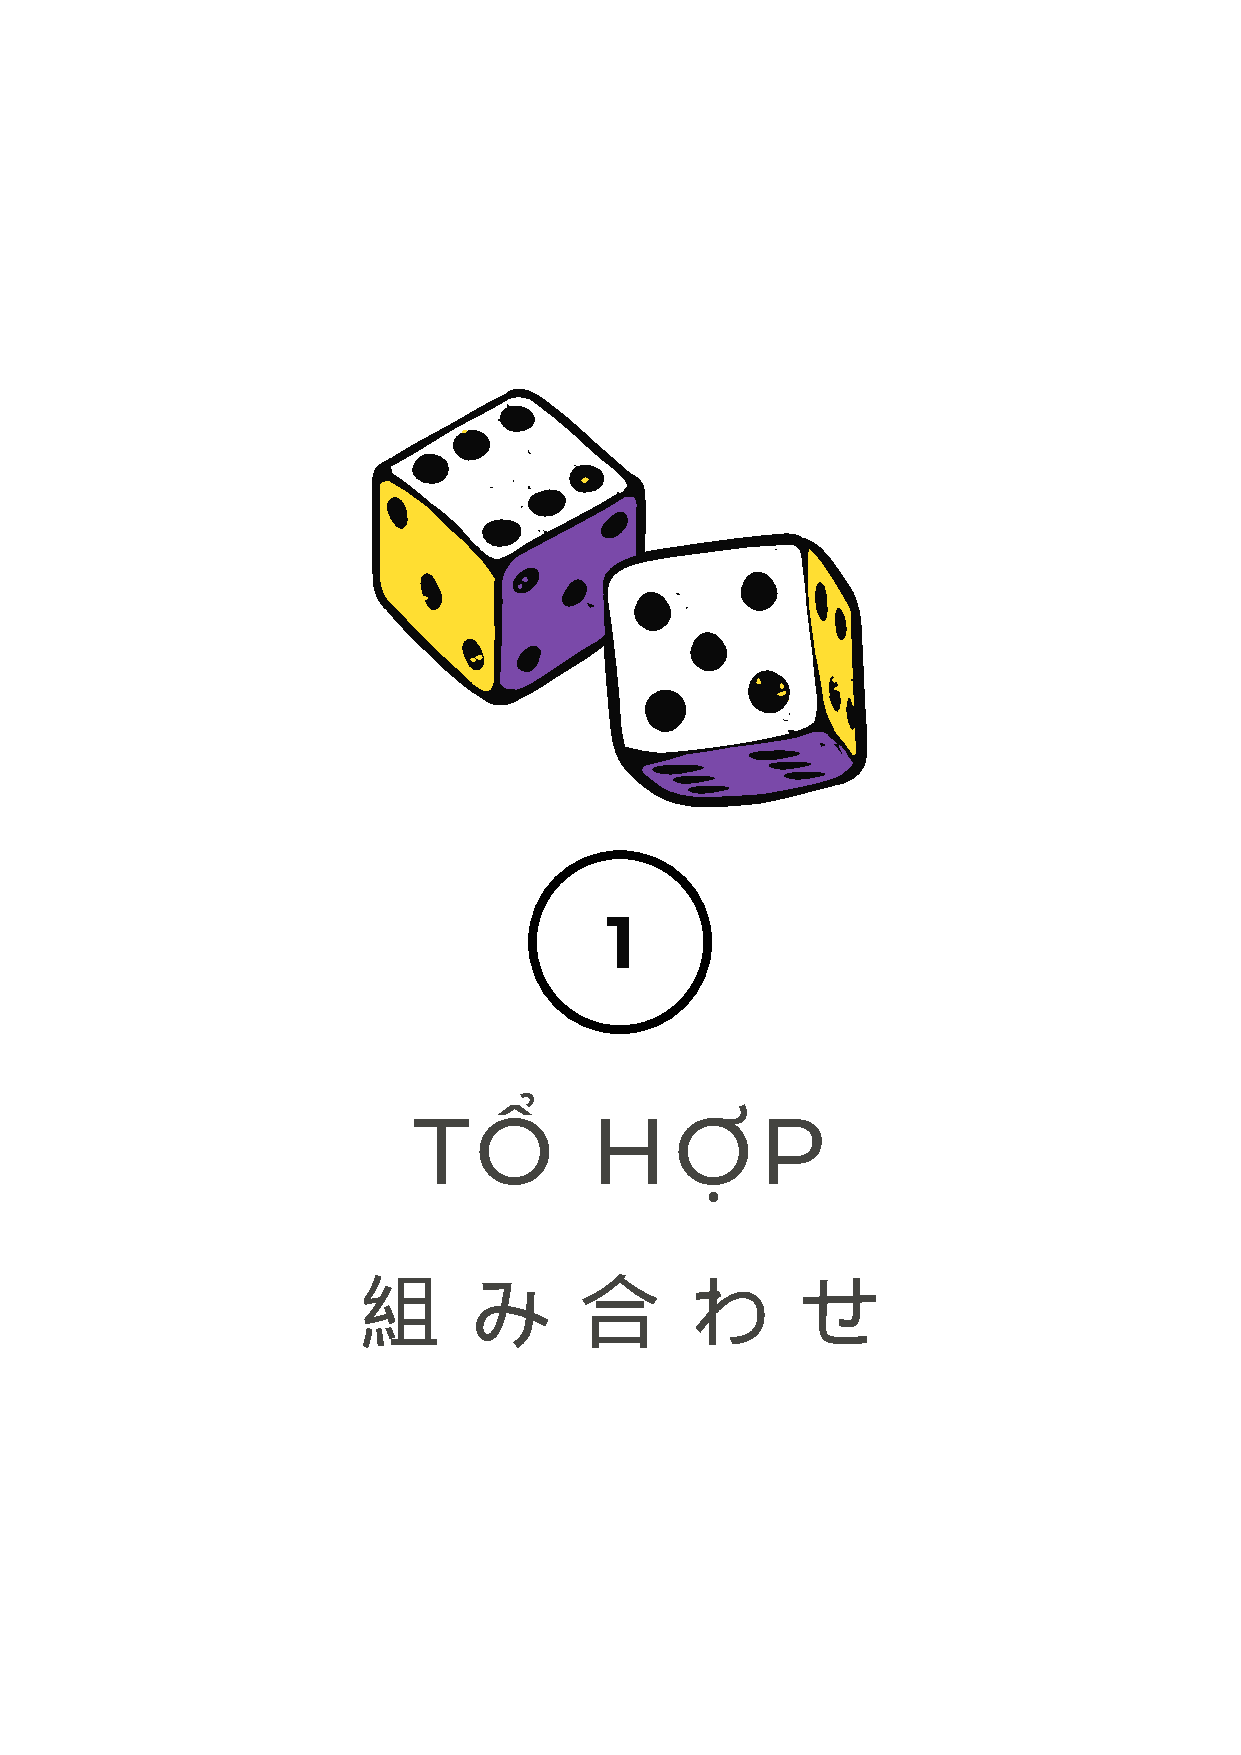
\includepdf[pages=1]{Image/bia/1.pdf}
\section{\huge Tổ hợp}
\subsection{\LARGE \textcolor{dk}{Đề bài}}

\setcounter{page}{1}
\thispagestyle{plain}
\begin{itemize}[label=, leftmargin=0em, itemsep=0.5em]
    
    \vspace{1em}
    \item \begin{bt}\vocab{(HMMT 02/2016).} Cho số nguyên lẻ $n > 1$. Trên một bàn cờ $n \times n$ có ô trung tâm và 4 ô ở góc bị cắt đi. Chúng ta muốn chia $n^2 -5$ hình vuông còn lại thành $\frac{1}{2}(n^2 - 5)$ cặp sao cho hai hình vuông ở mỗi cặp giao nhau tại chính xác một điểm. Tìm giá trị của $n$ thỏa mãn điều đó.
    \end{bt}
    \begin{sol}
        Ta tô màu xen kẽ cho bảng ô vuông bằng hai màu trắng và vàng, với hàng màu vàng nằm ở hàng trung tâm. khi đó sẽ có hai trường hợp như sau:
        \begin{center}
            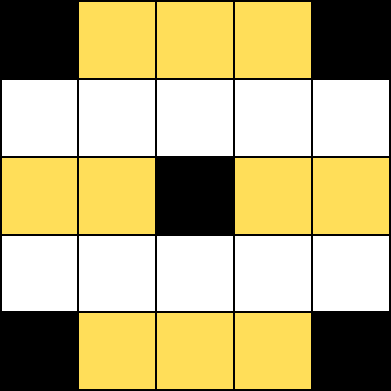
\includegraphics[scale=0.5]{Image/P1.1.pdf}
            \hspace{1cm}
            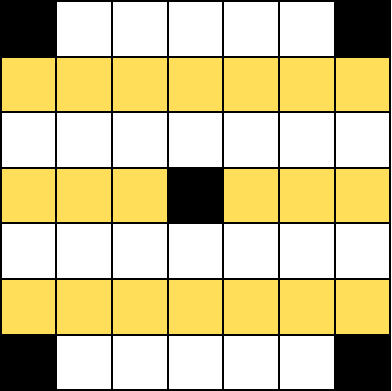
\includegraphics[scale=0.5]{Image/P1.2.pdf}
        \end{center}
        Mỗi cặp hình vuông thỏa mãn được chọn sẽ chiếm 1 ô trắng và 1 ô vàng, tức là để tồn tại một cách chọn thỏa mãn thì số ô vàng phải bằng số ô trắng.

        \vocab{Trường hợp 1:} hàng ở trên và dưới cùng được tô màu vàng.  Khi này tổng số ô màu vàng là $\frac{n(n + 1)}{2} - 5$, tổng số ô màu trắng là $\frac{n(n - 1)}{2}$, khi này ta được 
        \[
            \frac{n(n + 1)}{2} - 5 = \frac{n(n - 1)}{2} \lra n = 5
        \]
        \vocab{Trường hợp 2:} hàng ở trên và dưới cùng được tô màu trắng. Khi này tổng số ô màu vàng là $\frac{n(n - 1)}{2} - 1$, tổng số ô màu trắng là $\frac{n(n + 1)}{2} - 4$, khi này ta được 
        \[
            \frac{n(n - 1)}{2} - 1 = \frac{n(n + 1)}{2} - 4 \ra n = 3
        \]
        Vậy với $n \in \{3,5\}$ thì tồn tại cách chọn cặp thỏa mãn đề bài. Ta có một cách ghép cặp thỏa mãn như sau cho từng trường hợp:
        \begin{center}
            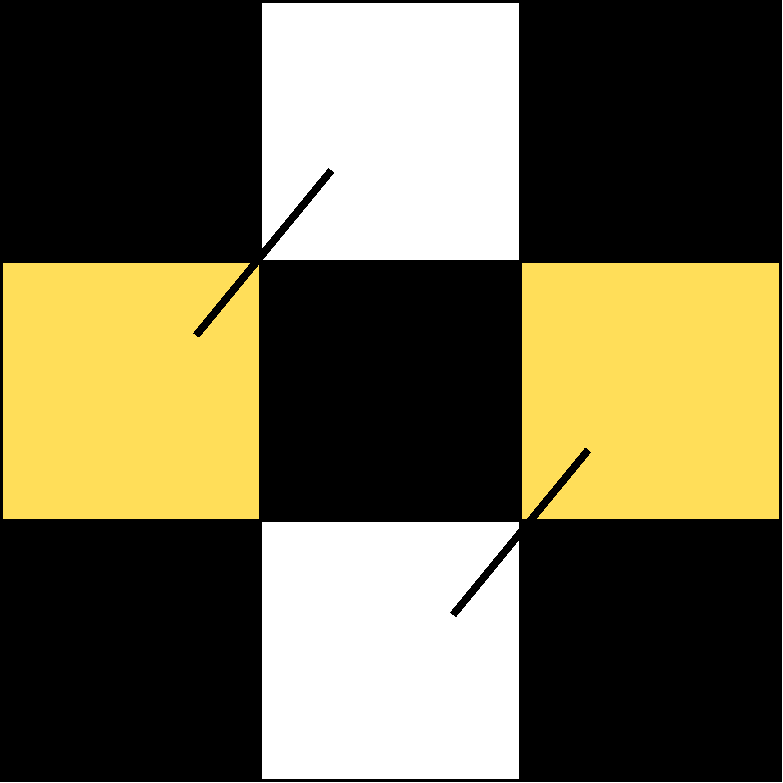
\includegraphics[scale=0.2]{Image/P1.3.pdf}
            \hspace{1cm}
            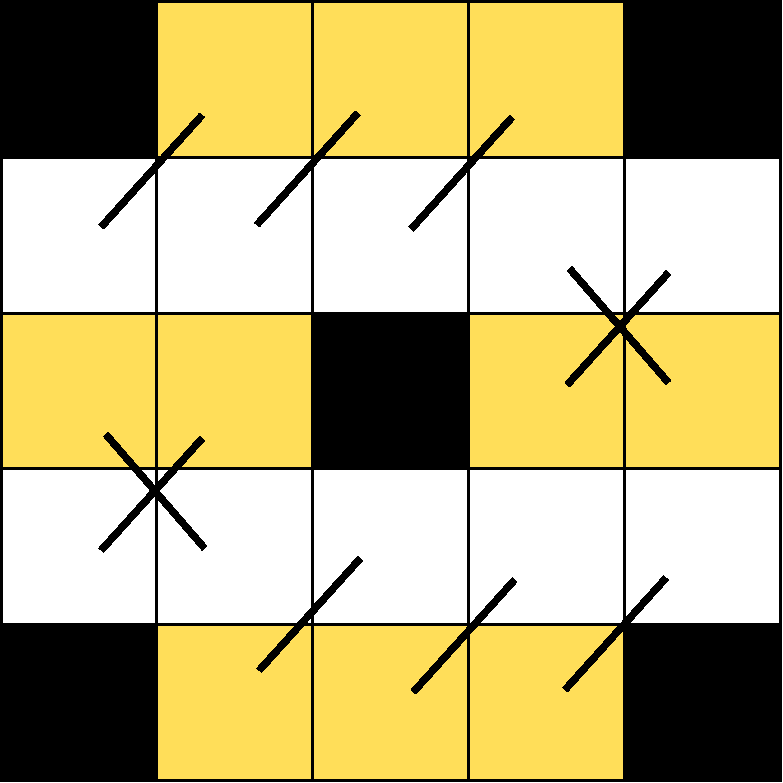
\includegraphics[scale=0.2]{Image/P1.4.pdf}
        \end{center}
    \end{sol}
    \newpage
    \item \begin{bt}\vocab{(USAJMO 2019).}
        Có $a+b$ cái bát được sắp xếp thành một hàng ngang, được đánh số từ $1$ đến $a+b$. Ban đầu, $a$ bát đầu tiên mỗi bát chứa một quả táo và $b$ bát cuối cùng mỗi bát chứa một quả lê.
        Một nước đi được gọi là \vocab{hợp lệ} bao gồm việc chuyển một quả táo từ bát $i$ sang bát $i+1$ và một quả lê từ bát $j$ sang bát $j-1$, với điều kiện là sự chênh lệch $i-j$ là chẵn. nhiều loại trái cây có thể nằm trong cùng một bát cùng một lúc. Mục tiêu là có được $b$ bát đầu tiên, mỗi bát chứa một quả lê và $a$ bát cuối cùng, mỗi bát chứa một quả táo. Chứng minh rằng điều này có thể xảy ra khi và chỉ nếu tích $ab$ là số chẵn.
    \end{bt}
    \begin{sol}
        \vocab{Nhận xét 1:} Tích $ab$ là số chẵn. Giả sử cả $a$ và $b$ đều lẻ. Ta nhận thấy rằng mỗi bước đi ta lấy táo và lê ở các bát cùng tính chẵn lẻ chuyển sang các bát bên cạnh. Thế nên ý tưởng bất biến đó là hiệu số táo và số lê ở ô lẻ. Thật vậy, tô đen các ô lẻ. 
        
        Ban đầu số táo ô đen là $\frac{a + 1}{2}$, số lê ô đen là $\frac{b - 1}{2}$, hiệu bất biến là $\frac{a - b + 2}{2}$. 
        
        Sau khi đạt được mục tiêu, số táo ô đen là $\frac{a - 1}{2}$, số lê ô đen là $\frac{b  + 1}{2}$, hiệu bất biến là $\frac{a - b - 2}{2}$, vô lý. Vậy nên tích $ab$ phải chẵn.

        \vocab{Nhận xét 2:} Với $ab$ chẵn thì luôn tồn tại nước đi hợp lý để đạt được mục tiêu. Ta sẽ chứng minh điều này đúng bằng quy nạp. Nếu $(a, b) = (0,b)$ hoặc $(a,b) = (1,b)$ thì rõ ràng luôn đúng. Giả sử giả thuyết đúng với mọi trường hợp $ \leq a + b - 2$ và $\min{a,b} \geq 2$. Ta có hai trường hợp:
        
        \vocab{Trường hợp 1: }$a + b$ chẵn. Xét $a + b$ ô. Ta đổi vị trí của táo ô $1$ và lê ô $a + b - 1$, táo ô $2$ và lê ô $a + b$, đưa về $(a - 2, b - 2)$, đúng theo quy nạp.
        
        \vocab{Trường hợp 2: }$a + b$ lẻ. Xét $a + b + 2$ ô. Ta đổi vị trí của táo ô $1$ và lê ô $a + b$, đưa về trường hợp $(a - 1, b - 1)$, đúng theo quy nạp.

        Như vậy là chứng minh hoàn tất.
    \end{sol}

    
    \item \begin{bt}\vocab{\href{https://www.facebook.com/ToanHocvoiPsi/posts/1319983838702201}{(KHTN Lớp 10 - 2023).}}
        Viết một trăm số nguyên dương đầu tiên $1,2,\dots,100$ vào một bảng ô vuông kích thước $10\times 10$ một cách tùy ý sao cho mỗi ô được viết đúng một số. Chứng minh rằng tồn tại hai ô kề nhau (2 ô có cạnh chung) mà hai số viêt ở hai ô này có hiệu lớn hơn hoặc bằng 10.
    \end{bt}
    \begin{sol}
        Giả sử với mọi hai ô kề nhau thì hiệu của chúng luôn bé hơn 10. Xét ba tập hợp sau 
        \[
            \begin{aligned}
                &A_x = \{1,2,\dots,x\}\\
                &B_x = \{x + 1, x+ 2,\dots,x +9\}\\
                &C_x = \{x + 10, x + 11,\dots, 100\}
            \end{aligned}
        \]
        với $x$ chạy trên $[2,90]$. Để ý rằng hai số kề nhau thì không thể nằm trong cả hai tập $A$ và $C$. Theo nguyên lý Dirichlet, sẽ tồn tại một hàng và một cột không chứa phần tử nào của $B$. Gọi hợp của hàng và cột đó là một "dấu cộng". Mọi số nằm trên dấu cộng sẽ chỉ có hai khả năng là toàn bộ thuộc $A$ hoặc $C$. Ta giả sử đó là $A$ thì $A \geq 19$. 

        Khi $x$ chạy trên $[1,90]$ thì dấu cộng sẽ thay đổi. Ta sẽ chứng minh rằng tồn tại một giá trị mà ở đó dấu cộng của $A$ sẽ biến thành của $C$ khi $x$ tăng một đơn vị, hoặc ngược lại. 
        
        Với $x = 2$ thì $A = 2 < 19$ nên dấu cộng của $x = 2$ sẽ chứa $C$. 

        Với $x = 90$ thì $C = 10 < 19$ nên dấu cộng của $x = 90$ sẽ chứa $A$.

        Khi này theo sự liên tục trong rời rạc thì sẽ tồn tại $i \in [2,90]$ để dấu cộng chứa $C$ tại $i$ và chứa $A$ tại $i + 1$.
        \begin{center}
            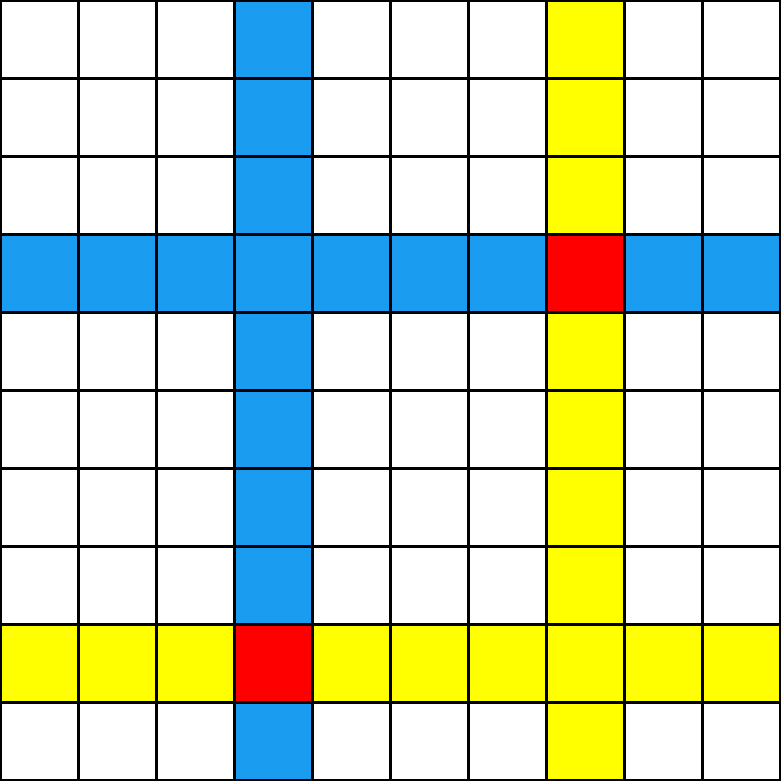
\includegraphics[scale=0.4]{Image/P3.pdf} 
        \end{center}
        
        Khi này thì hai dấu cộng sẽ giao nhau tại hai điểm. Mà lại khả năng $C$ hoặc $A$ mất đi một số nên sẽ tồn tại một số là giao của hai dấu cộng.
    \end{sol}
    

    \item \begin{bt}\vocab{(IMO 1993).} Trên bàn cờ vô hạn ta thực hiện một trò chơi như sau: Đầu tiên xếp $n^2$ quân vào một hình vuông gồm $n \times n$ ô vuông cạnh liền kề sao cho trong mỗi ô vuông của hình vuông chứa một quân cờ, cách đi trong trò chơi là quân cờ chỉ được nhảy theo một chiều ngang hoặc chiều dọc qua một ô có chứa quân cờ ở ngay sát bên cạnh sang một bên ô trống tiếp ngay sau đó. Khi đó quân cờ ô bị nhảy qua sẽ bị loại bỏ. Tìm các giá trị của $n$ để có thể kết thúc trò chơi sao cho trên bàn cờ chỉ còn lại đúng một quân cờ.
    \end{bt}
    \begin{sol}
        
        Tô xanh, đỏ, vàng xen kẽ cho bàn cờ. Gọi $A_1,A_2,A_3$ lần lượt là số quân cờ nằm ở ô xanh, đỏ, vàng.

        \vocab{Nhận xét 1: }$3 \nmid n$. 
        \begin{proof}
            Giả sử $3\mid n$, để ý rằng sau mỗi bước đi thì tính chẵn lẻ của $A_1,A_2,A_3$ bị thay đổi, để thắng trò chơi thì phải có một số bằng 1. Nhưng vì $A_1,A_2,A_3$ luôn cùng tính chẵn lẻ nên dẫn tới vô lý.
        \end{proof}

        \vocab{Nhận xét 2: } Với cấu hình sau thì có thể làm mất đi 3 quân ở cột trung tâm (với dấu $*$ tượng trưng cho mỗi quân cờ). Từ giờ ta sẽ gọi đây là nước đi $(\fa)$.
        \[
        \begin{bmatrix}
        . & * & . \\
        .& * & . \\
        . & * & *
        \end{bmatrix}
        \]
        \begin{proof}
            Di chuyển quân góc dưới phải $\to$ giữa trên $\to$ dưới trái.
        \end{proof}
        \vocab{Nhận xét 3:} Với $n = 1,2,4$ thì có thể thắng. Ta chỉ cần chứng minh với $n = 4$. Thực hiện liên tục $(\fa)$.
        \begin{proof}
        \[
        \begin{bmatrix}
        * & * & *&*\\
        * & * & *&*\\
        * & * & *&*\\
        * & * & *&*\\
        \end{bmatrix}
        \to 
        \begin{bmatrix}
            . & . & .&*\\
            * & * & *&*\\
            * & * & *&*\\
            * & * & *&*\\
        \end{bmatrix}
        \to 
        \begin{bmatrix}
            . & . & .&*\\
            . & . & .&*\\
            * & * & *&*\\
            * & * & *&*\\
        \end{bmatrix}
        \to 
        \begin{bmatrix}
            . & . & .&.\\
            . & . & .&.\\
            * & * & *&.\\
            * & * & *&*\\
        \end{bmatrix}
        \]
        \[
        \to 
        \begin{bmatrix}
            . & . & .&.\\
            . & . & .&.\\
            * & * & *&.\\
            * & * & *&*\\
        \end{bmatrix}
        \to 
        \begin{bmatrix}
            . & . & .&.\\
            . & . & .&.\\
            * & * & *&.\\
            * & . & .&.\\
        \end{bmatrix}
        \to 
        \begin{bmatrix}
            . & . & .&.\\
            . & . & .&.\\
            . & . & .&.\\
            * & . & .&.\\
        \end{bmatrix}
        \]
        \end{proof}
        \vocab{Nhận xét 4: } Từ $(n + 3)\times (n + 3)$ có thể đưa về $n \times n$.
        \begin{proof}
            Đối với mảng $3 \times k$ ở rìa ngoài, bằng nước đi $(\fa)$ ta có thể biến đổi như sau: 
            \[
                \begin{bmatrix}
                    * & * & *&*&*&*&...\\
                    * & * & *&*&*&*&...\\
                    * & * & *&*&*&*&...\\
                \end{bmatrix}
            \to 
                \begin{bmatrix}
                    . & * & *&*&*&*&...\\
                    . & * & *&*&*&*&...\\
                    . & * & *&*&*&*&...\\
                \end{bmatrix}
            \to 
                \begin{bmatrix}
                    . & . & *&*&*&*&...\\
                    . & . & *&*&*&*&...\\
                    . & . & *&*&*&*&...\\
                \end{bmatrix}
                \to \dots
            \]
            Khi đó khối $L$ $3 \times n$ ở phía ngoài đồng loạt thu về còn khối $4 \times 4$ ở góc, với một quân là giao của khối $4 \times 4$ và $n \times n$, và bằng nước đi ở nhận xét 3, ta đã quy về $n \times n$.
            \begin{center}
                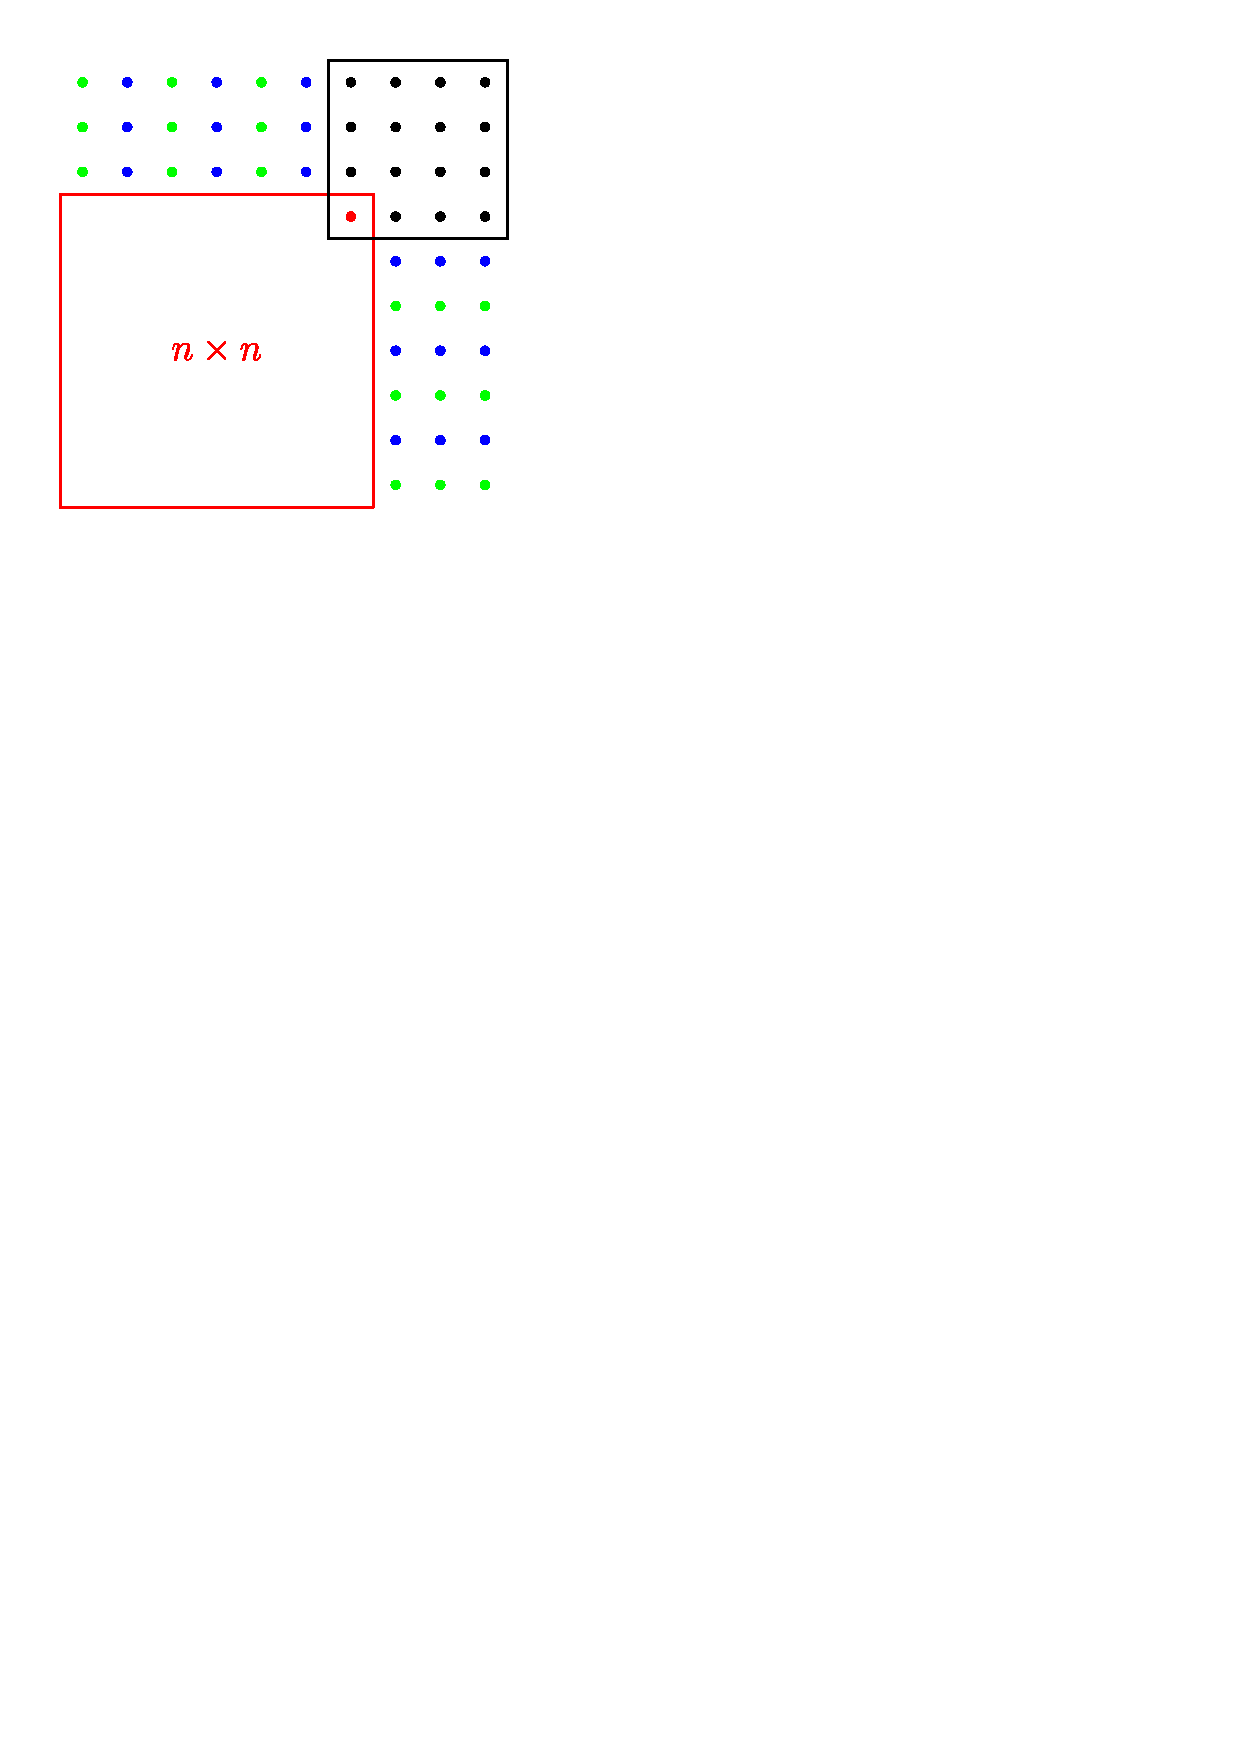
\includegraphics[scale=0.7]{Image/1993.pdf}
            \end{center}
            Mặt khác, với $n = 2,4$ thì có thể thắng, vì vậy theo quy nạp thì với $n = 3k + 1$ hoặc $n = 3k + 2$ với $k \geq 0$ thì có thể thắng.
        \end{proof}
    \end{sol}


\newpage
    \item \begin{bt}\vocab{(IMO Shortlist 2013 C1).}
        Cho $n$ là một số nguyên dương. Tìm số nguyên nhỏ nhất $k$ với tính chất sau: Cho bất kỳ các số thực $a_1 , \cdots , a_d $ sao cho $a_1 + a_2 + \cdots + a_d = n$ và $0 \le a_i \le 1$ với $i=1,2,\cdots ,d$, ta có thể phân chia các số này thành $k$ nhóm (một số trong số đó có thể là rỗng) sao cho tổng của các số trong mỗi nhóm không vượt quá $1$.
    \end{bt}
    \begin{sol}
        Ta sẽ tìm cách phân hoạch đủ lớn, sao cho mỗi nhóm của $k$ chỉ chứa ít nhất 1 phần tử để khi đó $k$ sẽ có chặn dưới tốt nhất. 
        
        Thật vậy, để có tồn tại phân nhóm ít nhất không thể phân được nữa thì mỗi phân hoạch $a_i$ phải lớn hơn $\frac{1}{2}$ để mỗi nhóm chỉ chứa đúng 1 phân hoạch.  Xét phân hoạch $a_i = \frac{1}{2} + \frac{1}{d}, \forall i = 1,2,\dots$.
        \[
        a_1 + a_2 + \dots + a_d = \frac{d}{2} + 1 = n
        \]
        Suy ra $d = 2n - 2$ và $k_{min} = 2n - 2$.
    \end{sol}

    
    \item\begin{bt}\vocab{(Japan MO Final 2016 P3). }
        Cho $n$ là một số nguyên dương. Trong vương quốc Skibidi có $2^n$ công dân và một vị vua. Trong ngôn ngữ tiền tệ, vương quốc sử dụng các tờ giấy bạc có mệnh giá là $2^n$ đồng và các đồng xu có mệnh giá là $2^a$ (với $a=0,1,\ldots,n-1$). Mỗi công dân có vô số tờ giấy bạc (không tính đến lạm phát). Gọi $S$ là tổng số đồng xu trong vương quốc. Một ngày đẹp trời, vua quyết định triển khai một chính sách sẽ được thực hiện mỗi đêm:
        \begin{enumerate}
            \item Mỗi công dân phải và anh ta phải chuyển một số tiền hữu hạn cho một công dân khác hoặc cho vua.
            \item Mỗi công dân phải chuyển chính xác nhiều hơn $\$1$ số tiền mà anh ta nhận được từ một công dân khác. 
            \item Luôn phải có một công dân kết thúc quá trình này bằng cách đưa tiền cho vua.
        \end{enumerate}

        Tìm giá trị nhỏ nhất của $S$ sao cho vua có thể thu tiền mỗi đêm mà không bao giờ hết tiền.
    \end{bt}

    \begin{sol}
        Tuy mỗi người có vô hạn tiền giấy, nhưng lại có hữu hạn xu. Vậy nên người cuối cùng đưa tiền cho vua phải đưa $k$ tờ tiền $2^n$ và ta gọi cách chuyển tiền này là $\mathbb{H}$. Ta hãy xét thuật toán như sau:

        Để chuyển tiền thỏa mãn $\mathbb{H}$, người đầu tiên phải đưa một số tiền bằng $k2^n$ với $k \geq 1$, vì ta muốn $S$ nhỏ nhất nên ta có thể tối ưu bằng cách để anh ta đưa $k$ tờ tiền giấy. Và mỗi người tiếp theo là $2,3,\dots,2^{n} - 1$ sẽ góp $\$1$ xu vào đến người thứ $2^n$ số tiền góp lại hiện tại là $(k + 1)2^n$ tính cả người thứ $2^n$ đã góp vào, vì tiền giấy của anh ta là vô hạn nên anh ta mcó thể đưa nhà vua $k + 1$ tờ tiền bao nhiêu lần cũng được.


        Khi này người thứ $2^n$ đang giữ $2^n$ đồng xu. Nếu ta chặn $S_{min} = 2^n$ thì sẽ có vài người ở lượt sau không có $\$1$ xu nên không thể chuyển tiền được.


        Vì vậy nên ta phải đưa cho mỗi người $t$ xu sao cho sau khi chọn $2^{n} - 1$ người làm người cuối cùng đưa tiền cho vua, thì người này vẫn có thể tiếp tục chuyển tiền được.


        Thật vậy, vì mỗi lần chuyển là tốn $\$1$ nên sau $2^{n}$ lần chuyển thì $t \geq 2^{n - 1}$


        Lấy tổng lại từng người thì ta được $S_{min} = n2^{n - 1}$, hoàn tất bài toán.\end{sol}

        \begin{bt}\vocab{(IMO Shortlist 2003)}
            Cho $A$ là một tập con gồm $101$ phần tử của tập $S=[1000000]$. Chứng minh rằng tồn tại các số $t_1$, $t_2, \ldots, t_{100}$ trong $S$ sao cho các tập\[ A_j=\{x+t_j\mid x\in A\},\qquad j=1,2,\ldots,100  \]là đôi một không giao nhau.
        \end{bt}
        \begin{sol}
            Xét tập hợp $D = \{x -y \mid x,y\in A\}$, khi đó hai tập $A_i$ và $A_j$ giao nhau khi và chỉ khi $t_i - t_j \in D$. Ngược lại, nếu $A_i \cap A_j = \varnothing$  thì khi đó $t_i - t_j \notin D$. Xét đồ thị $G = (V,E)$ có $10^6$ đỉnh, với mỗi đỉnh $v_i$ là tập $A_i$. Nếu $A_i \cap A_j = \varnothing$ thì có cạnh $ij$. Thật vậy, xét đỉnh $i$ bất kỳ. Để đỉnh $j$ kề $i$ thì $t_i - t_j \notin D$, thế nên chọn $j$ có $10^6 - |D| = 10^6 - 100.101$ cách. Suy ra $d(i) = 10^6 - 100.101$. Theo bổ đề bắt tay, ta có 
            \[
                |E(G)| = \frac{\dsum_{i = 1}^{10^6}d(i)}{2} = \frac{10^6(10^6 - 100.101)}{2} > \frac{98.10^{12}}{99.2}
            \]
            Theo định lý Turan, tồn tại một $K_{100}$ ở $G$. Nói cách khác, tồn tại các tập $A_i$ rời nhau, hoàn tất chứng minh.
        \end{sol}

    \item \begin{bt}\vocab{(PTNK 2020).}
        Một trường phổ thông có $n$ học sinh. Các học sinh tham gia vào tổng cộng $m$ câu lạc bộ $A_1,A_2,\dots,A_m$
        \begin{enumerate}[label=(\alph*)]
            \item Chứng minh rằng nếu mỗi câu lạc bộ có 4 học sinh và hai học sinh bất kì tham gia chung nhiều nhất 1 câu thì $m \leq \frac{n(n - 1)}{12}$
            \item Giả sử tồn tại $k > 0$ sao cho hai câu lạc bộ bất kỳ có chung nhau $k$ thành viên và tồn tại một câu lạc bộ $A_t$ có $k$ thành viên. Chứng minh rằng $m \leq n$.
        \end{enumerate}
    \end{bt}
    \begin{sol}

        (a) Ta đếm số bộ có cặp học sinh tham gia vào một CLB bằng hai cách 

        \vocab{Cách 1:} Mỗi CLB có 4 học sinh chọn ra 2 bạn, nên ta được 
        \[
            S = m\binom{4}{2} = 6m 
        \]
        \vocab{Cách 2:} Vì hai học sinh bất kỳ có chung tối đa 1 CLB nên ta được 
        \[
            S \leq \frac{n(n - 1)}{2}
        \]
        Thế thì $m \leq \frac{n(n - 1)}{12}$.

        (b) Vì CLB $A_t$ có $k$ thành viên và có chung $k$ thành viên với tất cả các CLB còn lại nên các thành viên $A_t$ đã tham gia tất cả CLB và cũng là thành viên chung của nhau. Xét $n - k$ học sinh còn lại thì mỗi học sinh phải tham gia tối đa 1 CLB (trong số các CLB còn lại), vậy nên số CLB không vượt quá $n - k$, nên suy ra $m \leq n - k + 1 \leq n$, hoàn tất chứng minh.
        
    \end{sol}
    \begin{bt}\vocab{(Japan MO Final 2017). }
        Cho số nguyên dương $n \geq 3$. Có $n$ người, mỗi ngày tổ chức một cuộc họp mà ít nhất 3 người tham dự. Mỗi người trong cuộc họp bắt tay với tất cả những người còn lại. Sau $n$ cuộc họp, mỗi cặp người đã bắt tay đúng một lần. Chứng minh rằng mỗi cuộc họp đều có cùng số người tham dự.
    \end{bt}
    Ta phát biểu hai lời giải theo ngôn ngữ lập luận và đồ thị. 
    \begin{sol}

        \vocab{Nhận xét 1:} Nếu $A$ không tham gia ngày thứ $m$ thì số ngày $A$ tham gia phải ít nhất bằng số người tham gia ngày thứ $m$''. 
        \begin{proof}
            Nếu những người ở ngày hôm đó đã bắt tay nhau, vậy nên họ không thể gặp lại lần nữa, tức để $A$ có thể bắt tay với tất cả những người đó thì phải có mặt ở những ngày mà những người đó có mặt.
        \end{proof}
        
        Ta sẽ đếm tổng số lượng người vào tất cả các ngày bằng hai cách.

        Không mất tính tổng quát, giả sử ngày thứ nhất có nhiều người tham gia nhất, và ngày thứ hai có nhiều người tham gia thứ nhì. Giả sử số người tham gia ngày 1 và ngày 2 lần lượt là $a$ và $b$, thì ta có số người tham gia nhiều nhất phải là $a + b(n - 1)$.


        Những người đã bắt tay vào ngày thứ nhất thì ngày thứ hai không thể xuất hiện cùng nhau, vì vậy có nhiều nhất một người $A$ tham gia cả ngày một và hai.


        Thế nên có $a - 1$ người ở ngày thứ nhất xuất hiện $b$ lần khác nhau và $A$ xuất hiện ít nhất 2 lần. Hơn nữa, những người không có mặt ở ngày thứ nhất sẽ xuất hiện ít nhất ở $a$ ngày. Vậy nên tổng số người tham gia ít nhất là $(a - 1)b + a(n-a) + 2$. Ta có bất đẳng thức 
        \[
            (a - 1)b + a(n - a) + 2 \leq a + b( n - 1) \lra (a - b)( n - a ) < a
        \]
        Nếu $a \neq b$ thế thì $n - a < a \lra a > \frac{n}{2}$
        
        
        Những người không có mặt vào ngày thứ nhất sẽ phải xuất hiện ít nhất trong $\frac{n}{2}$ ngày. Điều này rõ ràng là mâu thuẫn vì nếu người thứ nhất xuất hiện từ ngày $2$ đến $\frac{n}{2}$ thì người thứ hai phải xuất hiện ngày $\frac{n}{2}$ đến ngày $n$, xét đến người ba thì anh ta luôn xuất hiện nhiều lần hoặc với người đầu hoặc người thứ hai, mâu thuẫn.


        Điều này dẫn đến việc $a \leq \frac{n}{2} \lra n - a > a$. Để bất đẳng thức trên đúng thì $a = b$



        Mà thế thì mọi người đều phải tham gia ít nhất $a$ ngày nên vì thế số người tham gia mỗi ngày là như nhau, hoàn tất chứng minh.

    \end{sol}
    
    \vocab{Cách 2:} Bài toán có thể phát biểu lại như sau:
    \begin{lemma}
        Xét $G = (V,E)$ có $n$ đỉnh và không có cạnh. Mỗi một lần, lấy ra ít nhất 3 đỉnh đôi một độc lập nhau và nối chúng lại với nhau. Sau $n$ lần ta được một $K_n$ đầy đủ. Chứng minh rằng số đỉnh mỗi lần lấy là như nhau.
    \end{lemma}
    \begin{proof}
        
        Gọi $T_i$ là tập hợp các đỉnh ở lần lấy thao tác thứ $i$, $T = \{T_1,T_2,\dots,T_n\}$. Ký hiệu $T_i = |T_i|$. Gọi $A(u)$ là số lần xuất hiện của $u$ sau $n$ lần thao tác. 

        \vocab{Nhận xét 1:} Nếu $u \notin T_k$ bất kỳ thì $A(u) \geq T_k$.
        \begin{proof}
            Giả sử $A(u) < T_k$. Vì mỗi lần $T_k$ thì các cặp đỉnh không được chọn lại nên nếu $v_m,v_n \in T_k$ thì $\nexists j \in [n]: v_m,v_n \in T_j$. Mà vì $d(u) = n - 1$ nên sẽ tồn tại một đỉnh không kề $v$, vô lý.
        \end{proof}
        Không mất tính tổng quát, giả sử $T_1 = \max(T) = a, T_2 = \max(T \backslash \{T_1\}) = b$. Đặt $S = \dsum_{i = 1}^n T_i$. Giả thuyết rằng $a > b$.

        \vocab{Nhận xét 2:} $S \leq a +(n - 1)b$. 
        \begin{proof}
            Điều này có thể dễ dàng chứng minh bằng định nghĩa:
            \[
                S = T_1 + T_2 + \dots + T_n  \leq a + b + b + b +\dots + b = a + b(n - 1)
            \]
        \end{proof}
        \vocab{Nhận xét 3:}  $S \geq a(n - a) + b(a - 1)$
        \begin{proof}
            Để ý rằng $|T_1 \cap T_2| \leq 1$. Vì nếu không sẽ có $u,v \in T_1,T_2$ vô lý vì hai đỉnh bất kỳ chỉ được ghép 1 lần. 
            
            Khi này với $u  \notin T_1$ thì theo nhận xét 1 ta có $A(u) \geq a$. 
            
            Với $v \in T_1 \notin T_2$ thì sẽ có $A(v) \geq b$. 

            Tương tự với $w \in T_1 \cap T_2$ thì có $A(w) \geq 2$. Từ đó ta suy ra 
            \[
                S \geq a(n - a) + b(a - 1) + 2
            \]
        \end{proof}
        Kết hợp lại hai điều trên ta được 
        \[
        \begin{aligned}
            a + (n - 1)b \geq a(n - a) + b(a - 1) + 2 \lra a &\geq an -a^2 + ab  + 2 -nb\\
             &> (n - a)(a - b) \\
             &> n - a 
        \end{aligned}
        \]
        Suy ra $a > \frac{n}{2}$. Do đó với $u,v,w \notin T_1$ thì $A(u),A(v),A(w) > \frac{n}{2}$. Theo Dirichlet thì tồn tại hai trong số 3 đỉnh trên cùng xuất hiện nhiều hơn 2 lần, mâu thuẫn. Vậy nên $a = b$. Kéo theo $|T_1| = |T_2| =\dots = |T_n|$, hoàn tất chứng minh.
    \end{proof}
    \item \begin{bt}\vocab{\href{https://www.facebook.com/groups/vmo.tst/permalink/1373016430079150/}{(Đắk Lắk TST 2023).}}
        Tìm tất cả các tập hợp $A$ gồm 8 số nguyên dương sao cho với mọi số nguyên dương $n \leq 250$, tồn tại tập hợp $B$ là tập hợp con của $A$ thỏa mãn tổng tất cả các phần tử của $B$ bằng $n$.
    \end{bt}
    \begin{sol}
        Đặt $N = \{1,2,\dots,250\}$, nên $A \subset N$ ta có 
        \[
        \begin{aligned}
            1,2 &\in A\\
            3 = 1 + 2 &\in N\\
            4 &\in A\\
            5 = 3 + 2, 6 = 3 + 2 + 1, 7 = 4 + 3 &\in N\\
            8 \in A\\
            \dots
        \end{aligned}
        \]
        Ta dự đoán rằng $A = \{2^0,2^1,2^2,\dots,2^7\}$. Thật vậy, xét hàm số $f: N \to N_2$ biến một số thập phân bất kỳ thành số nhị phân. Ta chứng minh $f$ là hàm song ánh. Thật vậy, xét một số $a$ bất kỳ. Khi đó, thực hiện thuật toán chia $a$ cho $2$ đến khi $a \to 0$, theo Euclid ta được một dãy số dư duy nhất. Nếu tồn tại số $b$ có cùng dãy số dư với $a$ thì $a = b$. Suy ra $f$ đơn ánh. Hơn nữa với mọi $b_2$ thì luôn tồn tại $a$ để $f(a) = b_2$. Vậy nên $f$ song ánh.

        Mặt khác, giả sử tồn tại $t \neq 2^k, k \in 0,1,...,7$, mà $t \in A$, khi đó $t$ có thể phân tích theo nhị phân, nhưng vì $2^7 = 128 < 250$ nên $t \notin A$
         
        Vậy nên  $A = \{2^0,2^1,2^2,\dots,2^7\}$.
    \end{sol}
    \item \begin{bt}\vocab{(Phạm Bảo). }
        Cho tập hợp $S = \{1,2,...,n\}$ và $k$ là hằng số. Tìm số nguyên $f(n)$ nhỏ nhất để với mọi tập con của $S$ có $f(n)$ phần tử đều tìm được $k$ phần tử đôi một nguyên tố cùng nhau.
    \end{bt}
    \begin{sol} Đầu tiên để xét với mọi tập con hữu hạn mà có 2 số nguyên tố cùng nhau thì hai số này không thể có ước chung, tức là kích thước của tập phải lớn hơn số phần tử có ước chung của cả hai thì mới có thể bao hàm chúng được. Khi đó, ta có thể bù trừ các số có ước là $2,3,5,\dots$ dựa trên yêu cầu cần bao nhiêu số nguyên tố cùng nhau.
        Ta hãy xét một tập hợp và hàm số sau:
        \[
            \left\{
            \begin{array}{l}
                A_n = \{a \in \mathbb{S} \mid p_n \mid a \text{ và } p_{i} \nmid a, \forall i < n\}, \text{ với } p_i \text{ là số nguyên tố thứ } i\\
                h(n) = |A_n|
            \end{array}
            \right.
        \]
        Rõ ràng là $h(n)$ là hàm giảm trên khoảng nguyên tố $[2,+\infty)$ khi xét trên tập hữu hạn. Khi đó chặn dưới tốt nhất của $f$ sẽ là khi ta lấy hết tất cả các phần tử có ước chung với nhau. Do đó ta được
        \[
            f(n) \geq  h(2) + h(3) + ... + h(k) + 1 = \sum_{i = 2}^k h(i) + 1
        \]
        Thật vậy, ta có một bổ đề sau

        
        \begin{theo}[Bổ đề chia hết] -Cho một đoạn số nguyên $[a,b]$ và số nguyên $k$, khi đó có $\left\lfloor\frac{b - a + 1}{k}\right\rfloor$ số thuộc đoạn này chia hết cho $k$.
        \end{theo}
        Bổ đề có thể dễ dàng chứng minh được bằng nguyên lý Dirichlet.



        Đặt $T_i= \left\lfloor \frac{n}{i } \right\rfloor$. Để tính được $h(p_i)$ thì ta phải bù trừ các $T_i$ được tạo bởi các ước bé hơn nó. Ta có
        \[
            \begin{aligned}
                &h(1) = T_2 \\
                &h(2) = T_3 - T_6\\
                &h(3) = T_5 - T_{10} - T_{15} - T_{30}\\
                &...\\
                &h(i) = T_{p_i} - \sum_{j \in a_{p_i}} T_j,
            \end{aligned}
        \]
        với $a_{p_i}$ là bội và có các ước nguyên tố bậc 1 bé hơn $p_i$. Khi đó ta có
        \[
            \sum_{i = 2}^k h(i) + 1 = \left(\sum_{i = 1}^k T_{p_i}\right) - \left(\sum_{i = 1}^k \sum_{j \in a_{p_i}} T_{j}\right) + 1 = \sum_{i = 1}^k\left( T_{p_i} - \sum_{j \in a_{p_i}} T_{j}\right) + 1
        \]
        Kết luận lại, ta có $\displaystyle f(n)_{min} = \sum_{i = 1}^k\left( \left\lfloor \frac{n}{p_i }\right\rfloor - \sum_{j \in a_{p_i}} \left\lfloor \frac{n}{j }\right\rfloor\right) + 1$
        
    \end{sol}
    \vocab{Nhận xét:} Thông thường các giả thuyết như chứa số nguyên tố hay nguyên tố cùng nhau thì ta không có nhiều công cụ để xử lý trong tổ hợp. Vì vậy điều này gợi ý cho ta việc thực hiện điều ngược lại: Như thế nào thì hai số không nguyên tố cùng nhau? Làm cách nào để tránh điều đó?
    \item \begin{btvn}\vocab{(PTNK 2022).}
        Cho $n, k \geq 2$ là hai số nguyên dương và $a_0, a_1, \cdots, a_k$ là các số nguyên dương cho trước. Đặt $S_n=\{1,2, \cdots, n\}$, ta ký hiệu $A_n$ là số các bộ $\left(x_1, x_2, \cdots, x_k\right) \in S_n^k$ thỏa điều kiện:
        $$
        n \mid a_0+a_1 x_1+\cdots+a_k x_k .
        $$
        \begin{enumerate}[label=(\alph*)]
            \item Xét số nguyên tố $p \geq 5 ; a_0, a_1, \cdots, a_k$ phân biệt và đều nhỏ hơn $p$. Tính $A_{p^2}$.
            \item Tính $A_n$ với trường hợp tổng quát.
        \end{enumerate}
    \end{btvn}
    \item \begin{btvn}\vocab{(PTNK 2023).}
        Cho $n$ là một số nguyên dương. Một bảng ô vuông gôm $n$ hàng và $n$ cột gồm $n^2$ ô vuông đơn vị ta gọi là một bảng $n \times n$.
        Với mỗi số nguyên $k(1 \leq k \leq n)$, trên mỗi hàng ta chọn $k$ hàng liên tiếp và trên mỗi cột ta chọn $k$ cột liên tiếp, khi đó $k^2$ ô vuông nằm ở phần giao nhau ta gọi là một bảng con $k \times k$ của bảng $n \times n$ ban đầu.
        \begin{enumerate}[label=(\alph*)]
            \item Điền các số $1,2,3, \ldots, 81$ vào bảng $9 \times 9$. Chứng minh rằng tồn tại bảng con $2 \times 2$ có tổng của 4 số được điền trong nó lớn hơn 137.
            \item Giả sử $n$ là số lẻ. Mỗi ô vuông đơn vị của bàng $n \times n$ ta điền một số thuộc $\{-1 ; 0 ; 1\}$ sao cho mỗi bảng con $2 \times 2$ có tổng của 4 số được điền trong nó là 0 . Gọi $S$ là tổng của $n^2$ số trong bảng $n \times n$. Tìm giá trị lớn nhất của $S$.
        \end{enumerate}
    \end{btvn}
    \begin{bt}\vocab{(Yufei Zhao).}
        Cho $X$ là một tập hữu hạn có $|X| = n$, và gọi $A_1, A_2, \dots, A_m$ là các tập con của $X$ có ba phần tử sao cho $|A_i \cap A_j| \le 1$ cho tất cả $i \neq j$. Chứng minh rằng tồn tại một tập con $B$ của $X$, có ít nhất $\sqrt{2n}$ phần tử, sao cho $X \nsupseteq  A_i$ với mọi $i \in [n]$.
    \end{bt}
    \begin{sol}
        Đặt $A = (A_1 \cup A_2 \cup \dots \cup A_m)$
        Giả sử $\exists k_{min}: |B| \geq k$ và $B \nsupseteq A_i, \forall i \in [n]$. Khi này ta có thể đếm $A$ bằng hai cách.
        \begin{enumerate}
            \item  \vocabf{Cách 1 (theo phần bù):} Trường hợp $A$ nhỏ nhất chắc chắn là khi các $A_i$ đều không lấn sang $B$, và ta có được $A \geq n - k $ 
            \item \vocabf{Cách 2 (Đếm quét cực đại): }Giả sử $\exists x_i \in B$ sao cho $x \cup A_i \subset A$. Theo giả thuyết đề bài thì mỗi $|A_i \cap A| = 2$ và $|A_i \cap B| = 1$. Cho nên $|A| \leq \dbinom{k}{2}$
        \end{enumerate}
        Tổng kết lại thì $$n - k \leq \dbinom{k}{2} \Leftrightarrow  k^2 + k \geq 2n \Rightarrow \Delta \lra 4 + 8n \Rightarrow k \geq \frac{-1 + 2\sqrt{1 + 2n}}{2} \geq \sqrt{2n}$$
    \end{sol}
    \begin{bt}
        Trên trục số nguyên, một con ếch xuất phát tại 0, nhảy đến các vị trí có tọa độ thuộc $\left\{1,2,3, \ldots, 2^{2022}-1\right\}$, mỗi điểm được nhảy qua không quá một lần và con ếch có thể nhảy tới hoặc nhảy lùi lại tùy ý. Biết rằng độ dài bước nhảy của ếch là lũy thừa của 2 và gọi $a_k$ là số bước nhảy độ dài $2^k$ mà con ếch đã nhảy.
    \begin{enumerate}[label=(\alph*)]
        \item Chứng minh rằng $a_{2021} \leq 2^{2021}$ và $a_{2021}+a_{2020} \leq 3 \cdot 2^{2020}$.
        \item Tìm giá trị lớn nhất của tổng $S$ độ dài tổng từng các bước nhảy theo mỗi lũy thừa của ếch có thể thực hiện được(xét theo từng độ dài).
    \end{enumerate}
    \end{bt}
    \begin{sol}
        \begin{enumerate}
            \item Ta để ý rằng số các bước không quá $2^{2022} -1 $ không thể nào có 2 bước liên tiếp có độ dài $2^{2021}$ vì nếu không kiểu gì cũng sẽ lố $2^{2022} - 1$. Cho nên chỉ có 1 bước mỗi lần như vậy, hay nói cách khác, mỗi bước $2^{2021}$ phải được xen kẽ bởi một bước nhỏ hơn và trường hợp tốt nhất là $2^0 = 1$, như vậy ta sẽ có được:
            $$
            a_{2021} \leq \left\lceil \frac{2^{2022} - 1}{2}\right\rceil   = 2^{2021}
            $$
            Tiếp theo ta cần chứng minh $a_{2021} + a_{2020} \leq 3.2^{2020}$. Để ý rằng thì không có 4 bước liên tiếp nào có độ dài nào là $2^{2020},2^{2021}$, thì đó cứ 3 bước như ta xen kẽ 1 bước đơn vị tương tự như trên, và mặt khác mỗi 3 bước thì hẳn phải có 3 lựa chọn thì ta có được:
            $$
            a_{2021} + a_{2020} \leq 3\left\lceil \frac{2^{2022} - 1}{4}\right\rceil = 3.2^{2020}
            $$
            \item Ta xét số bước khả thi của $a_k$ thì đương nhiên, không thể nào ta đi $2^{2022 - k}$ lần $a_k$ được, thì khi đó cứ $2^{2022 - k} - 1$ bước $a_k$ thì ta bước 1 bước đơn vị, khi đó ta được
            $$
            a_k \leq \left\lceil \frac{2^{2022} - 1}{2^{2022 - k}} \right\rceil = 2^k
            $$
            Từ đó số độ dài các bước nhảy cực đại là:
            $$
            S = \sum_{i = 0}^{2021} 2^i a_i \leq \sum_{i=0}^{2021} 4^i = \frac{4^{2021}- 1}{3}
            $$
            \end{enumerate}
    \end{sol}
    \begin{bt}\vocab{(Japan MO Final 2018 P1). }
        Cho các số nguyên dương từ $1$ đến $100$ được viết trên một bảng đen, mỗi số đúng một lần. Một phép toán bao gồm việc chọn hai số $a$ và $b$ trên bảng đen và xóa chúng, sau đó viết số ước chung lớn nhất của $a^2+b^2+2$ và $a^2b^2+3$. Sau một số lượng phép toán, chỉ còn lại một số nguyên dương trên bảng đen. Chứng minh rằng số này không thể là số chính phương.
    \end{bt}

    \begin{sol}
        Ta chứng minh rằng tính chia hết cho $3$ là bất biến. 
        
        Nếu $3 \mid a,b$ thì khi đó $3\nmid a^2 + b^2 + 2$ nên $3 \nmid \gcd(a^2 + b^2 + 2, a^2b^2 + 2)$


        Nếu $3 \nmid a,b$ thì $3\nmid a^2b^2 +3$ nên $3 \nmid \gcd(a^2 + b^2 + 2, a^2b^2 + 2)$


        Nếu chỉ có $a$ hoặc $b$ chia hết cho $3$, khi đó ta có hai trường hợp


        Nếu $b = 3k + 1, k \in \mathbb{Z}$ thì khi đó $a^2 + b^2 + 2 = a^2 + 9k^2 + 6k + 1 + 2 \equiv 0 \pmod{3}$


        Nếu $b = 3k + 2, k \in \mathbb{Z}$ thì khi đó $a^2 + b^2 + 2 = a^2 +9k^2 + 6k + 4 + 2 \equiv 0 \pmod{3}$


        Khẳng định được chứng minh.


        Mặt khác dễ dàng kiểm tra được rằng $ 9 \nmid \gcd(a^2 + b^2 + 2, a^2b^2 + 2)$


        Mặt khác vì từ 1 đến 100 có $33$ số chia hết cho 3 và có 100 lượt nên tức là đến một lúc nào đó sẽ chỉ còn $33$ số chia hết cho 3, và sau chẵn lượt tất nhiên là sẽ được một số chia hết cho 3, mà số này lại không chia hết cho 9 nên không thể là số chính phương.
    \end{sol}

    \begin{bt}\vocab{(Japan MO Final 2019). }
        Cho $n \geq 3$ là một số lẻ và xét một lưới ô vuông $n\times n$. Trò chơi bao gồm $n^2$ lượt, ở mỗi lượt, chúng ta sẽ thực hiện các thao tác sau theo tuần tự.
        \begin{enumerate}
            \item Chúng ta sẽ chọn một ô chứa một số nguyên chưa được viết và viết một số nguyên từ 1 đến $n^2$. Chúng ta chỉ có thể viết một số nguyên một lần duy nhất trong suốt trò chơi.
            \item Đối với mỗi hàng, cột bao gồm cả một ô, nếu tổng vài số nguyên  nằm trên hàng, cột hoặc một ô là bội số của $n$, thì chúng ta sẽ nhận được 1 điểm.
        \end{enumerate}
        Xác định giá trị lớn nhất có thể của điểm số như tổng số có thể đạt được vào cuối trò chơi.
    \end{bt}

    \begin{sol}
        Lấy module $n$ các số và ta sử dụng $n$ thay vì $0$. 
        Ta gọi $r_i$ và $c_i$ lần lượt là tổng các số thuộc hàng hoặc cột $i$. Khi đó số điểm lớn nhất mà hàng $i$ có thể nhận được là $\left\lfloor \frac{r_i}{n} \right\rfloor$. Khi này số điểm lớn nhất ở hàng là 
        \[
            \sum_{i = 1}^n \left\lfloor \frac{r_i}{n} \right\rfloor \leq \frac{\dsum_{i = 1}^n r_i}{n} = \frac{n(n + 1)}{2}
        \]
        Lý do tổng vẫn theo mod $n$ là vì số điểm khi này phải phụ thuộc vào các số mod $n$. Tương tự với cột thì ta có tổng điểm lớn nhất là $n(n +1)$. Giờ ta sẽ chỉ ra một cấu hình có thể đạt được giá trị lớn nhất. Viết vào ô $(i,j)$ với $i<n$ số $i$ nếu $2\nmid j$ và $n-i$ ngược lại và viết $n$ vào hàng cuối cùng.
    \end{sol}

    \item \begin{btvn}\vocab{(Japan MO Final 2021).}
        Cho số nguyên dương $n \geq 2$. Hai người chơi $A$ và $B$ chơi một trò chơi trên lưới các ô vuông đơn vị $n \times 2021$. Đầu tiên, $A$ tô mỗi ô màu đen hoặc trắng. $B$ đặt một viên bi vào một trong các ô ở hàng trên cùng và chỉ định một trong các ô ở hàng dưới cùng làm \textit{goal}. Sau đó, $A$ thao tác $n - 1$ lần như sau:
        \begin{enumerate}
            \item Khi ô có bi được sơn màu trắng, $A$ di chuyển bi sang ô bên dưới.
            \item Nếu không, $A$ hãy di chuyển viên bi đến ô tiếp theo ở bên trái hoặc bên phải, sau đó đến ô bên dưới.
            
        \end{enumerate}
        
        Tìm giá trị nhỏ nhất của $n$ sao cho $A$ luôn có thể di chuyển một viên bi đến \textit{goal}, bất kể lựa chọn của $B$.
    \end{btvn}

    \begin{bt}\vocab{(Japan MO Final 2022).}
        Có $2022$ ô vuông được đánh số thứ tự trên một hàng ngang. Hai người $A$ và $B$ cùng nhau chơi một trò chơi. Đầu tiên, những ô vuông số lẻ được đánh dấu chữ $A$ và những ô vuông số chẵn được đánh dấu chữ $B$. Sau đó, bắt đầu từ $A$, họ thay phiên thực hiện những thao tác sau:
        \begin{enumerate}
            \item Người chơi sẽ chọn hai ô vuông được đánh dấu bằng tên của họ, sao cho hai ô đó không kề nhau, và tất cả các ô vuông nằm ở giữa hai ô đó đều được đánh dấu bằng tên của đối thủ và đổi tên tất cả các ô đó sang tên của mình.
            \item Hai người chơi luân phiên chơi liên tục như vậy đến khi có một người không thể thao tác tiếp được nữa
        \end{enumerate}
        Tìm số nguyên dương $m$ lớn nhất sao cho $A$ luôn có thể đảm bảo rằng có ít nhất $m$ ô vuông được đánh dấu chữ $A$.
    \end{bt}

    \begin{sol}
        Ta có thể tổng quát bài toán này. Gọi $f(n)$ là số ô vuông lớn nhất $A$ có thể đảm bảo là có tên mình trên lưới $2n \times 1$.


        Xét lưới $2n \times 1$ thì bởi vì $A$ đi đầu nên bất kể $A$ chọn vị trí nào đồng nhất, ta có thể xem $AAA$ ở lượt đầu là $A$ khi này kích thước lướt trở thành $2(n - 1) \times 1$ mà trong khi đó số lượng $A$ và $B$ vẫn là như nhau xen kẽ. Cấu hình này chính bằng $f(n - 1)$. Do đó ta lập được hệ thức truy hồi:
        \[
            \left\{
                \begin{array}{l}
                    f(1) = 1, f(2) = 3\\
                    f(n) = f(n - 1) + 1
                \end{array}
            \right.
        \]
        Thế nên tìm được $f(n) = n$. Có được $f(1011) = 1011$. Bây giờ ta sẽ thiết lập một chiến thuật dành cho $A$ để luôn có thể đảm bảo ít nhất được con số này. 


        Đầu tiên $A$ sẽ bắt đầu thao tác từ trái sang, anh ta có thể thực hiện như sau:
        \[
            \begin{aligned}
                &ABABAB\dots AB \to AAABAB\dots AB \to AAABAB\dots BBB\dots AB\\
                &\to AAAAAB\dots BBB \dots AB \to \dots
            \end{aligned}
        \]
        Số lượng chữ $A$ được thể hiện như sau:
        \[
            1011 \to 1012 \to 1011 \to 1012 \to\dots
        \]
        Có thể thấy rằng bất kể $B$ chọn ở đâu để đồng nhất thì $A$ luôn giữ được một lượng quân nhất định từ bên trái sang và chúng chỉ có thể tăng mà không giảm được dưới $1011$, hoàn tất bài toán.
    \end{sol}

    \item \begin{btvn}\vocab{(Japan MO Final 2023).}
        Trên một bảng ô vuông $5 \times 5$, người ta đặt các Tetromino
        lên các hình vuông để trong mỗi hình vuông, có hai hoặc ít hơn viên được bao phủ (các viên này có thể xếp chồng lên nhau). Tìm số hình vuông lớn nhất được bao phủ bởi đúng một viên.
    \end{btvn}


    \item \begin{btvn}\vocab{(Japan MO Final 2024).}
    Trong mặt phẳng tọa độ, các điểm có tung độ và hoành độ nguyên thuộc $1$ đến $2000$ được gọi là điểm tốt. Hơn nữa, đối với bốn điểm $A(x_1, y_1)$, $B(x_2, y_2)$, $C(x_3, y_3)$, $D(x_4, y_4)$ có đường đa tuyến $ABCD$ được gọi là đường $\mathbb{Z}$ nếu như:
    \begin{enumerate}
        \item Tất cả đều $A, B, C, D$ là những điểm tốt.
        \item  $x_1<x_2$, $y_1=y_2$
        \item $x_2>x_3$, $y_2-x_2=y_3-x_3$
        \item $x_3<x_4$, $y_3=y_4$
    \end{enumerate}
    
    Tìm giá trị nguyên dương $n$ nhỏ nhất sao cho có $n$ đường $\mathbb{Z}$ là $Z_1, Z_2,\dots, Z_n$ thỏa mãn với bất kỳ điểm $P$ tốt nào, tồn tại một số nguyên $i \in [n]$ sao cho $P$ nằm trên $Z_i$.
        
    \end{btvn}
    \begin{bt}\vocab{(Nguyễn Tuấn Anh). }
        Cho $\mathcal{S}$ là tập hợp các bộ số nguyên dương $(x_1,x_2,\dots,x_n)$ là nghiệm của phương trình
    \[
        x_1 + x_2 +\dots+x_n = n^n
    \]
    Tính giá trị của biểu thức
    \[
        T=\sum_{(x_1,x_2,\dots,x_n) \in S}x_1x_2\dots x_n 
    \]
    \end{bt}


    \begin{sol}
        \vocab{Cách 1: Đếm bằng hai cách}


        \vocab{Cách thứ 1: }Đếm theo tập hợp. Ta phân chia $n^n$ số vào $n$ tập hợp $A_1, A_n,\dots A_n$ khác rỗng. Khi này lực lượng của các tập phải thỏa mãn
        \[
            |A_1| + |A_2| + \dots + |A_n| = n^n
        \]
        Mỗi tập ta chọn ra một phần tử thì theo quy tắc nhân ta có $x_1x_2\dots x_n$ cách. Chung quy lại
        \[
            T=\sum_{(x_1,x_2,\dots,x_n) \in S}x_1x_2\dots x_n 
        \]
        \vocab{Cách thứ 2:} Phân hoạch nguyên. Ta xếp các số $1,2\dots,n^n$ lên một đường thẳng từ trái sang phải. 


        Khi này ta sẽ thực hiện thao tác phân hoạch đoạn số nguyên này và mỗi đoạn chọn một số. Thao tác phân hoạch $\to$ chọn $\to$ phân hoạch $\to \dots$ $\to$ phân hoạch $\to$ chọn ($2n - 1$ bước) có thể được hiểu là một cách chọn ra $2n - 1$ số trên và ta chèn cấu hình đó vào. 
        
        
        Tuy nhiên, nếu một số được chọn với vai trò là để phân hoạch thì ta đã vô tình loại nó ra nên không thể chọn được, vì vậy, ta sẽ cần thêm $n - 1$ đối tượng làm phân hoạch, để có thể hiểu rằng mỗi lần chọn phân hoạch là ta đang chọn một trong các đối tượng đó. Và có được số cách thao tác trên là
        \[
            T = \binom{n^n + n - 1 }{2n - 1}
        \]
        So sánh hai cách đếm ta hoàn tất bài toán.


        \vocab{Cách 2: Sử dùng hàm sinh}


        Ta xét hàm sinh
        \[
            f(x) = \left(\sum_{i = 0}^{\infty}ix^i\right)^n
        \]
    \end{sol}
    \begin{bt}\vocab{(Korean\ MO 2023).}
        Cho các tập hợp $A_0, A_1, \dots, A_{2023}$ thỏa mãn các điều kiện sau:
        \begin{enumerate}
            \item $A_0 = \{ 3 \}$
            \item $A_n = \{ x + 2 \mid x \in A_{n -     1} \} \ \cup \{x(x+1) / 2 \mid x \in A_{n - 1} \}$ với mọi $n = 1, 2, \dots, 2023$.
        \end{enumerate}
    Tính $|A_{2023}|$.  
    \end{bt}

    \begin{sol}
        Giả sử tồn tại hai dãy phép toán có cùng độ dài biến $3$ thành cùng một số. Giả sử số đó là $\frac{2k(2k + 1)}{2} = 2k^2 + k$


        Ta được hai số trước đó là $2k^2 + k - 2$ và $2k$.


        Xét số $\frac{2k(2k - 1)}{2}$ thì cần tối thiểu $k - 1$ phép toán để trở thành $2k^2 + k$ tuy nhiên điều này là không thể vì khi đó để được $2k$ thì phải xuất phát lớn nhất là $2$ vô lý. Vậy nên 
        \[
            \{ x + 2 \mid x \in A_{n - 1} \} \ \cap \{x(x+1) / 2 \mid x \in A_{n - 1} \} = \varnothing
        \]
        Khi đó ta được $|A_{2023}| = 2^{2023}$.
    \end{sol}

    \item \begin{btvn}\vocab{(Đồng Tháp TST 2022).}
        Trên đường tròn có 2023 điểm phân biệt. Tìm số nguyên dương $n$ nhỏ nhất sao cho với mọi cách chọn $n$ điểm trong số các điểm trên, tồn tại hai điểm sao cho phần trong của một trong hai cung tròn có đầu mút là hai điểm nói trên chứa đúng 1012 điểm trong số 2023 điểm đã cho (phần trong của một cung tròn là các điểm của cung đó không kể hai đầu mút).
    \end{btvn}
    \item \begin{bt}\vocab{(India TST 2010).}
        Cho bảng vuông $10\times 10$, mỗi ô $(i,j)$ được điền bởi một số thực dương $a_{ij}$ sao cho tổng các số thuộc mỗi hàng, mỗi cột của bảng luôn là $1$. Chứng minh rằng tồn tại $j,k,l,m \in [10]$ với $j < k$ và $l < m$ sao cho
        \[
            a_{jl}a_{km} + a_{jm}a_{kl} \geq \frac{1}{50}
        \]
    \end{bt}
    \begin{sol}
        Rõ ràng 4 điểm nói trên tạo ra một hình chữ nhật nằm trong bảng ô vuông đó (tổng tích các cạnh đối lớn hơn hoặc bằng $\frac{1}{50}$)\\
    - Ta sẽ giả sử rằng với mọi bốn điểm như vậy thì hệ thức trên luôn bé hơn $\frac{1}{50}$\\
    Ta đếm tổng giá trị các phần tử của tập hợp
    $$ S = \{a_{jl}a_{km} + a_{jm}a_{kl} \}$$
    \begin{itemize}[label=,leftmargin=0em]
        \item \textbf{Cách 1:} Chọn ra hai dòng bất kì và từ một trong hai dòng đó chọn ra 2 điểm, ta tạo được một hình chữ nhật. Ta được $$|S| < \frac{1}{50}\binom{10}{2}\binom{10}{2} $$
                    \begin{figure}[ht]
            \centering
            \subfloat{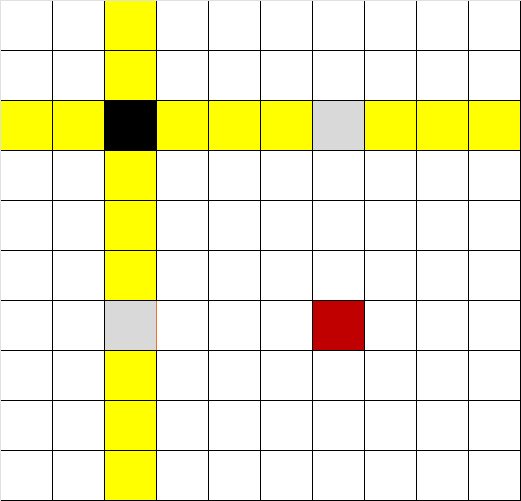
\includegraphics[width=0.3\linewidth]{Image/ando.png}}
        \end{figure}
        \item \textbf{Cách 2:} Đếm dựa trên một điểm $a_{ij}$ cho trước. Ta sẽ tìm một điểm $b_{mn} $ nào đó để tạo nên một đường chéo. 
        
        Khi đó nếu ta lấy $\sum a_{ij}b_{mn}$ và nhân 2 lên chia cho 4 thì ta được S, vì mỗi lần chọn cặp $(a,b)$ thì ta chọn ra 2 đường chéo, tức là sau khi đếm hết thì mỗi đường chéo được đếm hai lần. 
    
        - Nhưng nếu đếm như vậy thì mỗi cấu hình của S sẽ lặp lại 4 lần, tức là ô màu đen và đỏ đổi vị trí cho nhau, ô màu đen và đỏ thế chỗ cho 2 ô xám, ta được 4 cấu hình như nhau.
    
        Gọi $S_{ij}$ là tổng giá trị các phần tử trong $S$ có chứa $a_{ij}$. Ta được $$S_{ij} = a_{ij} \sum b_{mn}$$
        Chọn $a$ có 100 cách. Theo hình vẽ bên trên thì những chỉ những ô màu trắng mới chứa được $b$, nên do đó $b$ có $100 - 10 - 9 = 81$ cách, viết lại 
        $$ S_{ij} = a_{ij}\sum_{1}^{81} b_{mn}
        $$
        Nếu nhìn vào bảng thì ta còn có thể làm gọn tổng này hơn nữa. Ta có
        $$ S_{ij} = a_{ij}[10 - 1 - (1 - a_{ij}) ]
        = a_{ij}(8 + a_{ij})
        = a_{ij}^2 + 8a_{ij}
        $$
        Cộng lại các $S_{ij}$ ta được
        $$ |S| = \frac{1}{2}\sum_{1}^{100} S_{ij} =\frac{1}{2} \sum_{1}^{100} a_{ij}^2 + 8a_{ij} =  \frac{1}{2}.8.10 + \frac{1}{2}\sum_{1}^{100} a_{ij}^2  
        $$
        Áp dụng bất đẳng thức Cauchy-Schwartz ta có 
        $$ \sum_{i=1}^{100} a_{ij}^2 \geq \frac{ \left(\displaystyle \sum_{i=1}^{100}a_{ij}\right)^2}{100} = 1
        $$
        Do đó $|S| \geq \frac{1}{2}.80.10 + \frac{1}{2} = \frac{81}{2}$
    \end{itemize}
    Từ đây cho ta được mâu thuẫn bài toán, suy ra điều phải chứng minh.
    \end{sol}

    \item \begin{bt}\vocab{(Đồng Tháp TST 2023).}
        Bạn Bảo có $n$ cái hộp, lần lượt chứa $1,2,\dots,n$ viên bi ($n > 1$). Bạn Bảo thực hiện việc cho thêm bi vào hộp theo các quy tắc sau:
        \begin{enumerate}
            \item Ở lượt đầu tiên, bạn ấy cho thêm vào mỗi hộp 1 viên bi.
            \item Ở lượt thứ hai, với các hộp có số bi chia hết cho $2$, bạn ấy sẽ thêm vào mỗi hộp đó 1 viên bi.
            \item Cứ như vậy, ở lượt $k$, nếu có hộp nào với số bi chia hết cho $k$, bạn Bảo sẽ thêm vào mỗi hộp đó 1 viên bi.
        \end{enumerate}
        Tìm tất cả các số nguyên $n > 1$ sao cho kết thúc lượt thêm bi thứ $n$ thì mỗi hộp đều có đúng $n + 1$ viên bi.
    \end{bt}
    \begin{sol}
         Ký hiệu tập $\{1,2,\dots, n\}$ là $[n]$ với mọi $n$ nguyên dương.

        \vocab{Nhận xét 1:} $n + 1$ là số nguyên tố 
        \begin{proof}
            Giả sử $n + 1$ là hợp số, khi đó tồn tại $p \in \bb{P}$ sao cho $p \mid n + 1$, khi đó ở lượt thứ $1$ và $p$, hộp thứ $n$ sẽ chứa $n + 2$ viên bi, vượt mức cho phép.

            Vậy nên $n + 1$ là số nguyên tố.
        \end{proof}
        Xét một hộp thứ $k >1$ bất kỳ, gọi $f(x): [n] \to [n]$ là số viên bi của hộp $k$ ở lượt thứ $x$. Đặt $g(x) = f(x) - x - 1$. 
        
        
        \vocab{Nhận xét 2:} $f$ và $g$ là hàm liên tục trên tập rời rạc $[1,n]$.
        \begin{proof}
          Mỗi lượt chỉ được thêm vào hộp 1 viên bi, khi đó ta có  
        \[
         0 \leq f(x + 1)  - f(x) \leq 1 \ra |f(x + 1) - f(x)| \leq 1, \forall x \in [n]
        \]
        Mặt khác lại có 
        \[
        \begin{aligned}
            &0 \leq g(x + 1) + x + 2 -g(x) -x - 1\leq 1\\
            & \ra -1 \leq g(x + 1) - g(x)\leq 0\\
            & \ra |g(x + 1) - g(x)| \leq 1
        \end{aligned}
        \]
        Suy ra $f$ và $g$ liên tục trên $[1,n]$.
        \end{proof}
        \vocab{Nhận xét 3:} $f(x) \leq n + 1, \forall x \in [n]$
        \begin{proof}
            Giả sử tồn tại $t$ sao cho $f(t) > n + 1$, vì $n + 1$ nguyên tố nên để đạt được từ $n + 1$ lên $n + 2$ viên bi thì phải chơi nhiều hơn $n + 1$ lượt, mâu thuẫn.
        \end{proof}
        \vocab{Nhận xét 4:} Tồn tại $a$ để $g(a) = 0$. 
        \begin{proof}
            Thật vậy, vì $k > 1$ nên khi đó $g(1) = k - 2 \geq 0$. Mặt khác lại có $k \leq n$ nên $g(n) = f(n) -n - 1\leq n + 1 - n -1= 0$. 
            
            Khi đó $g(1).g(n) \leq 0$ và vì $g$ liên tục nên theo định lý giá trị trung gian thì tồn tại $a \in [n]$ để $g(a) = 0$.
        \end{proof} 
        \vocab{Nhận xét 5:} Với $a \in [1,n]$ thỏa mãn $g(a) = 0$ thì $f(t) = t + 1,\forall t \geq a$.
        \begin{proof}
            Thật vậy ở lượt thứ $a$ thì số bi ở hộp $k$ là $a + 1$. Nên ở lượt $a + 1$ thì hộp $k$ có $a + 1$ viên nên tăng 1 viên, lặp lại như vậy, thì ta được $f(t) = t + 1, \forall t \geq a$.
        \end{proof}
        Khi này vì $n \geq t \geq a$ nên $f(n) = n + 1$. Vậy nên mỗi hộp sau $n$ lượt có đúng $n + 1$ viên bi khi và chỉ khi $n + 1$ là số nguyên tố.
    \end{sol}
    \item \begin{btvn}\vocab{\href{https://artofproblemsolving.com/community/c5h2156986p15952792}{(USOMO 2020).}}
        Giả sử $(a_1,b_1),$ $(a_2,b_2),$ $\dots,$ $(a_{100},b_{100})$ là các cặp được sắp xếp khác nhau của các số nguyên không âm. Đặt $N$ là số các cặp số nguyên $(i,j)$ thoả mãn $1\leq i<j\leq 100$ và $|a_ib_j-a_jb_i|=1$. Xác định giá trị lớn nhất có thể của $N$ qua tất cả các lựa chọn có thể của $100$ cặp được sắp xếp.
    \end{btvn}

    \item \begin{btvn}\vocab{\href{https://artofproblemsolving.com/community/c5h1824275p12195834}{(Yannick Yao).}}
        Hai số hữu tỉ \(\tfrac{m}{n}\) và \(\tfrac{n}{m}\) được viết trên một bảng đen, với \(m\) và \(n\) là các số nguyên dương tương đối nguyên tố. Tại bất kỳ thời điểm nào, Evan có thể chọn hai số \(x\) và \(y\) được viết trên bảng và viết số trung bình cộng \(\tfrac{x+y}{2}\) hoặc số trung bình nghịch đảo \(\tfrac{2xy}{x+y}\) của chúng lên bảng. Tìm tất cả các cặp \((m,n)\) sao cho Evan có thể viết 1 lên bảng trong một số bước hữu hạn.
    \end{btvn}
    \item \begin{btvn}\vocab{(Kon Tum TST 2023).}
        Trên một đường tròn có đường kính bằng 2, người ta tiến hành tô đỏ một số cung tròn không có điểm chung. Cho $d$ là một đường kính tùy ý của đường tròn. Chứng minh rằng luôn tồn tại dây cung song song $d$ sao cho cả hai đầu mút của dây cung đó đều được tô màu đỏ. Biết rằng tổng độ dài của các cung màu đỏ lớn hơn $\pi$
    \end{btvn}
    \item \begin{btvn}\vocab{(Tiền Giang TST 2023).}
        Năm bạn học sinh thông minh ngồi xung quanh một chiếc bàn tròn. Thầy giáo đưa cho các em một số quả táo và nói với các em: "Thầy đưa cho một số các em một số quả táo, không có hai em nào có cùng số táo. Hơn nữa, mỗi em sẽ biết số táo của mỗi bạn trong hai bạn ngồi cạnh mình (bạn ngồi cạnh bên trái và bạn ngồi cạnh bên phải)". Sau đó thầy giáo nói cho các em học sinh tồng số táo mà các bạn học sinh có và đề nghị các em học sinh đoán hiệu số táo của hai bạn ngồi đối diện vơi mình (hai bạn không ngồi cạnh mình).
        \begin{enumerate}[label=(\alph*)]
            \item Chứng minh rằng thầy giáo có cách đưa cho năm học sinh tổng cộng 16 quả táo để không bạn nào có thế đoán được chính xác hiệu số được hỏi.
            \item Giả sừ tổng số táo nhỏ hơn 16. Chứng minh rằng có ít nhất một học sinh đoán được chính xác hiệu số được hỏi.
        \end{enumerate}
    \end{btvn}
    \item \begin{btvn}\vocab{(Thanh Hóa TST 2023).} a) Tại ô vuông nằm ở vị trí trung tâm của một bảng ô vuông kích thước $11 \times 11$ (bảng gồm 121 ô vuông có cạnh là 1) có một quân cờ. Mỗi bước đi, quân cờ di chuyển đến ô vuông có chung cạnh. Có bao nhiêu cách đi để sau 10 bước đi thì quân cờ trờ về vị trí ban đầu? Biết rằng trong quá trình di chuyển quân cờ có thể đi qua ô vuông nằm ở vị trí trung tâm.
    

        b) Chọn ra một số tập con gồm 4 phần tử từ một tập hợp $A$ có 36 phần tử sao cho bất cứ hai tập 4 phần từ nào trong các tập con đã chọn cũng có nhiều nhất là hai phần tử chung. Chứng minh rằng tồn tại một tập con của $A$ gồm ít nhất 6 phần từ của $A$ sao cho tập này không chứa bất cứ tập con 4 phần tử nào đã chọn.
    \end{btvn}
    \item \begin{btvn}\vocab{(An Giang TST 2023).}
        Cho lục giác lồi $A_1 A_2 A_3 A_4 A_5 A_6$ có diện tích bằng 1 và có các cặp cạnh đối diện song song, hai đường thẳng $A_6 A_1 ; A_2 A_3$ cắt nhau tại các điểm $B_1$, hai đường thẳng $A_1 A_2 ; A_3 A_4$ cắt nhau tại điểm $B_2 ; \ldots ;$ tương tự $A_{i-1} A_i ; A_{i+1} A_{i+2}$ cắt nhau tại điểm $B_i, i=1 \ldots 6\left(\right.$ xem $A_7$ là $A_1$ và $A_8$ là $\left.A_2\right)$. Chứng minh rằng tổng diện tích sáu tam giác $A_i B_i A_{i+1} ; i=1 \ldots 6$ không bé hơn 1.
    \end{btvn}
    \item \begin{btvn}\vocab{(Bình Phước TST 2023).}
        Trên bàn có 99 tấm thẻ được đánh số từ 1 đến 4 và từ 6 đến 100 . Hai bạn $A$ và $B$ luân phiên chơi trò chơi với luật như sau:
        \begin{enumerate}
            \item A là người thực hiện lượt chơi đầu tiên.
            \item Trong mỗi lượt chơi, người chơi nhặt ra khỏi bàn 2 tấm thė được đánh hai số nguyên liên tiếp nhau sao cho số bé hơn không chia hết cho 10 và giữ một tấm thè trên tay đồng thời bỏ đi tấm thẻ còn lại.
            \item Khi tới lượt chơi của mình, nếu người chơi không thể thực hiện được yêu cầu ii hoặc chọn được hai tấm thè nhưng tổng số của một trong hai tấm thè đó với một tấm thẻ tuỳ ý trên tay hai người chơi đang giữ bằng 101 thì là người thua cuộc.
        \end{enumerate}
        Biết rằng hai người chơi có thể thấy được số ghi trên tất cả các tấm thẻ trên bàn và trong tay đối thủ. Hỏi ai là người có chiến thuật thắng.
    \end{btvn}
    \item \begin{btvn}\vocab{(Hong Kong TST 2009).}
        Trong một trường học có $2008$ học sinh. Học sinh là thành viên của một số ủy ban nhất định. Một ủy ban có tối đa $1004$ thành viên và mỗi hai học sinh tham gia vào một ủy ban chung.
        \begin{enumerate}
            \item Xác định số ít nhất có thể của các ủy ban trong trường học.
            \item Nếu yêu cầu thêm rằng hợp của bất kỳ hai ủy ban nào cũng không được vượt quá $1800$ học sinh, thì câu trả lời trong (i) có đúng không?
        \end{enumerate}
    \end{btvn}
    \item \begin{btvn}\vocab{(Vinh 2023).} Có $k$ người trong một gia đình đi nghỉ mát trong thời gian 7 ngày tại khu du lịch. Buổi sáng, mỗi người chọn ăn một trong 3 món: xôi, phở hoặc bánh mỳ. Biết rằng trong bất kỳ 3 ngày nào, cũng có ít nhất một người mà trong 3 ngày này chọn ăn 3 món phân biệt. Tìm giá trị nhỏ nhất có thể của $k$.
        
    \end{btvn}
    
    \item \begin{btvn}\vocab{(OLP 30/4/2021)}
    Bộ hai số nguyên khác không $(x, y)$ được gọi là "bộ số đẹp" nếu $x$ là số lẻ, $y$ là số chẵn, $x, y$ nguyên tố cùng nhau và $x^2 - y^2$ là số chính phương.
    \begin{enumerate}
        \item Chứng minh rằng $(x, y)$ là "bộ số đẹp" khi và chỉ khi tồn tại 2 số nguyên $u, v$ khác $0$ và khác tính chẵn lẻ, nguyên tố cùng nhau sao cho $(x, y) = (u^2 - v^2, 2uv)$.
        \item Với mỗi bộ số đẹp $(x, y)$ ta có thể tạo ra 1 bộ số đẹp mới bằng 1 trong 2 phép biến đổi: hoặc đổi dấu của 1 trong 2 số hoặc cộng 1 số nguyên $k$ nào đó vào cả 2 số sao cho $(x + k, y + k)$ là bộ số đẹp. Chứng minh rằng với bất kỳ bộ số đẹp $(x, y)$ và $(z, t)$ cho trước ta luôn có thể biến đổi từ $(x, y)$ thành $(z, t)$ sau hữu hạn các bước biến đổi như trên.
    \end{enumerate}
    
    \end{btvn}
    \item \begin{btvn}\vocab{(OLP 30/4/2023). } Ký hiệu $(a_1, a_2, \ldots, a_{2023})$ là một hoán vị của tập hợp $X = \{1; 2; \ldots; 2023\}$ thỏa mãn tính chất $2(a_1 + a_2 + \ldots + a_k)$ chia hết cho $k$ với mọi $k = 1, 2, \ldots, 2023$.
        \begin{enumerate}
            \item Chứng minh $a_{2023} \in \{1, 2023\}$.
            \item Tính số các hoán vị trên.
        \end{enumerate}
    \end{btvn}

    \item \begin{btvn}\vocab{(Đồng Nai TST 2023).}
        Cho các ý sau:
        \begin{enumerate}[label=(\alph*)]
            \item Cho $2024$ viên bi được xếp thành hàng ngang. Tính số các cách đặt $29$ chiếc thẻ vào giữa các viên bi thỏa mãn ở giữa hai viên bi kề nhau chỉ có nhiều nhất một chiếc thẻ và các viên bi đã cho được thành $30$ phần, mà mỗi phần có ít nhất $9$ viên bi.
            \item Cho 2024 viên bi giống nhau được đặt vào các đỉnh của hình đa giác đều có $2024$ cạnh nội tiếp đường tròn $(O)$, mỗi đỉnh chỉ có 1 viên bi. Tính số các đặt 29 chiếc thẻ giống nhau vào trung điểm các cạnh của đa giác đã cho thỏa mãn tại mỗi trung điểm có nhiều nhất một chiếc thẻ và các viên bi đã cho được chia thành $29$ phần, mà mỗi phần có ít nhất 9 viên bi (biết hai cách đặt thẻ được coi là như nhau nếu tồn tại phép quay quanh tâm $O$ biến cách chia này thành cách chia kia).
        \end{enumerate}
    \end{btvn}
    \item \begin{btvn}\vocab{(Hà Tĩnh TST 2023).}
        Cho $n$ số nguyên dương đôi một phân biệt $a_1,a_2,\dots,a_n$. Chứng minh rằng với mọi $i \in [n]$, tồn tại số nguyên dương $b$ sao cho $ba_i$ là lũy thừa của số nguyên dương với số mũ lớn hơn $1$.
    \end{btvn}

   
    \item \begin{btvn}\vocab{(RMM 2019).}
        Hai con kiến đang di chuyển dọc theo các cạnh của một đa diện lồi. Đường đi của mỗi con kiến kết thúc tại điểm bắt đầu của nó, sao cho một con kiến không đi qua cùng một điểm hai lần trên đường đi của mình. Trên mỗi mặt $F$ của đa diện được viết số cạnh của $F$ thuộc về đường đi của con kiến đầu tiên và số cạnh của $F$ thuộc về đường đi của con kiến thứ hai. Có một đa diện và một cặp đường đi mô tả như trên, sao cho chỉ có một mặt chứa một cặp số khác nhau không?
    \end{btvn}
    \item \begin{btvn}\vocab{(APMO 2022).}
        Cho \( n \) và \( k \) là hai số nguyên dương. Cathy đang chơi trò chơi sau đây. Có \( n \) viên bi và \( k \) hộp, với các viên bi được đánh số từ \( 1 \) đến \( n \). Ban đầu, tất cả các viên bi được đặt trong một hộp. Mỗi lượt, Cathy chọn một hộp và sau đó di chuyển các viên bi có số nhỏ nhất, nói là \( i \), đến một hộp trống hoặc hộp chứa viên bi \( i+1 \). Cathy thắng nếu tại bất kỳ thời điểm nào có một hộp chỉ chứa viên bi \( n \).

        Xác định tất cả các cặp số nguyên \( (n,k) \) sao cho Cathy có thể thắng trò chơi này.

    \end{btvn}
    \item \begin{btvn}\vocab{(Taiwan MO 2024).}
        Cho \( n \) và \( k \) là các số nguyên dương. Một em bé sử dụng \( n^2 \) khối để tạo thành một lưới \( n \times n \), với mỗi khối có một số nguyên dương không lớn hơn \( k \). Bố đi ngang qua và nhận thấy rằng:

        1. Mỗi hàng trên lưới có thể được xem như một dãy số học với số bên trái là số hàng đầu tiên, với tất cả chúng đều có hiệu số chung khác nhau;
        
        2. Mỗi cột trên lưới có thể được xem như một dãy số học với số trên cùng là số cột đầu tiên, với tất cả chúng đều có hiệu số chung khác nhau.

        Tìm giá trị nhỏ nhất có thể của \( k \) (dưới dạng một hàm của \( n \)).

    \end{btvn}
    \item \begin{btvn}\vocab{(VMO 2009).}
        Hãy xác định số lượng tập con $T$ của $S$ sao cho không có hai phần tử nào trong $T$, $a$ và $b$, thỏa mãn điều kiện $|a-b|=\{1,n\}$, trong đó $S =\{1,2,3, \ldots, 2n\}$ và $n \in \mathbb{Z}^+$.
    \end{btvn}

    \item \begin{btvn}\vocab{(VMO 2010).}
        Cho số nguyên dương $n$. Xem xét bảng vuông $3 \times 3$. Sử dụng $n$ màu để tô màu tất cả các ô của bảng sao cho:
        \begin{enumerate}
            \item Mỗi ô được tô màu bởi đúng một màu.
            \item Hai bảng được tô màu giống nhau nếu chúng có thể được nhận từ nhau bằng cách quay một góc $90^\circ$ hoặc $270^\circ$ quanh trung tâm của bảng $3 \times 3$.
        \end{enumerate}
    Có bao nhiêu cách tô màu cho bảng vuông này thỏa mãn các điều kiện trên?
    \end{btvn}

    \item \begin{btvn}\vocab{(Vietnam TST 2010).}
        Chúng ta có $n$ quốc gia. Mỗi quốc gia có $m$ người sống trong nước đó ($n>m>1$). Chúng ta chia $m \cdot n$ người thành $n$ nhóm mỗi nhóm có $m$ thành viên sao cho không có hai người nào trong bất kỳ nhóm nào đến từ cùng một quốc gia.


        Chứng minh rằng có thể chọn $n$ người vào một lớp sao cho họ đến từ các nhóm và các quốc gia khác nhau.
    \end{btvn}

    \item \begin{btvn}\vocab{(VMO 2011).}
        Cho một đa giác lồi $ABCDE$ thoả mãn độ dài các cạnh và $AC, AD \leq \sqrt{3}.$ Chọn $2011$ điểm phân biệt bên trong đa giác này. Chứng minh rằng tồn tại một đường tròn đơn vị có trung tâm trên một cạnh của đa giác, và chứa ít nhất $403$ điểm trong số $2011$ điểm đã cho.

    \end{btvn}

    \item \begin{btvn}\vocab{(Vietnam TST 2011).}
        Cho $n$ là một số nguyên lớn hơn $1.$ $n$ học sinh được sắp xếp xung quanh một bàn tròn, mỗi người có một số kẹo nhất định (có thể có trường hợp một số học sinh không có kẹo) sao cho tổng số kẹo mà họ sở hữu là bội số của $n.$ Họ trao đổi kẹo như sau: 
        
        \begin{enumerate}
            \item Đối với số kẹo ban đầu của mỗi học sinh, ít nhất có một học sinh có nhiều kẹo hơn học sinh ngồi bên phải của mình, trong trường hợp đó, học sinh bên phải sẽ được nhận một viên kẹo từ học sinh đó.
            \item Sau một vòng trao đổi, nếu có ít nhất một học sinh có kẹo nhiều hơn học sinh bên phải, thì học sinh đó sẽ trao một viên kẹo cho học sinh tiếp theo ngồi bên phải của mình.
        \end{enumerate}  
        Chứng minh rằng sau khi trao đổi kẹo hoàn tất (tức là khi đạt đến cân bằng), tất cả học sinh có cùng số kẹo.
    \end{btvn}

    \item \begin{btvn}\vocab{(VMO 2012).}
        Cho một nhóm gồm 5 cô gái, ký hiệu là $G_1,G_2,G_3,G_4,G_5$ và 12 chàng trai. Có $17$ ghế được sắp xếp thành một hàng. Các học sinh đã được nhóm để ngồi trên ghế sao cho các điều kiện sau được đồng thời thỏa mãn:
        \begin{enumerate}[label=(\alph*)]
            \item Mỗi ghế có một người ngồi.
            \item Thứ tự, từ trái sang phải, của các cô gái ngồi là $G_1; G_2; G_3; G_4; G_5.$
            \item Giữa $G_1$ và $G_2$ phải có ít nhất ba chàng trai.
            \item Giữa $G_4$ và $G_5$ phải có ít nhất một chàng trai và tối đa bốn chàng trai.
            
        \end{enumerate} 
    Có bao nhiêu cách sắp xếp như vậy là có thể?
    \end{btvn}

    \item \begin{btvn}\vocab{(Vietnam TST 2012).}
    Xét một lưới chữ nhật có kích thước $m\times n$ với $m$ hàng và $n$ cột. Có các đài phun nước trên một số ô của lưới. Một đài phun nước có thể phun nước lên bất kỳ ô kề cạnh nào, hoặc một ô trong cùng một cột sao cho có đúng một ô giữa chúng. Tìm số lượng đài phun nước tối thiểu sao cho mỗi ô có thể được phun nước trong các trường hợp:
    \begin{enumerate}[label=(\alph*)]
        \item $m=4$
        \item $m=3$
    \end{enumerate}
    \end{btvn}

    \item \begin{btvn}\vocab{(VMO 2013).}
        Viết xuống một số lượng số $a_1, a_2, \ldots, a_n$ từ trái sang phải trên một dòng. Bước 1, chúng ta viết $a_1+a_2$ giữa $a_1,a_2$; $a_2+a_3$ giữa $a_2,a_3$, …, $a_{n-1}+a_n$ giữa $a_{n-1},a_n$, và sau đó chúng ta có dãy mới $b=(a_1, a_1+a_2,a_2,a_2+a_3,a_3, \ldots, a_{n-1}, a_{n-1}+a_n, a_n)$. Bước 2, chúng ta làm điều tương tự với dãy $b$ để có dãy mới $c$ lại.... Và tiếp tục như vậy. Nếu chúng ta thực hiện 2013 bước, hãy đếm số lượng số 2013 xuất hiện trên dòng nếu
        \begin{enumerate}[label=(\alph*)]
            \item $n=2$, $a_1=1, a_2=1000$
            \item $n=1000$, $a_i=i, i=1,2\ldots, 1000$
        \end{enumerate}
    \end{btvn}

    \item \begin{btvn}\vocab{(Vietnam TST 2013).}
        Một khối lập phương có kích thước $10\times 10\times 10$ bao gồm $1000$ khối đơn vị, tất cả được tô màu trắng. $A$ và $B$ chơi một trò chơi trên khối lập phương này. $A$ chọn một số trụ có kích thước $1\times 10\times 10$ sao cho không có hai trụ nào chia sẻ một đỉnh hoặc một cạnh, và chuyển tất cả các khối đơn vị được chọn thành màu đen. $B$ được phép chọn một số khối đơn vị và hỏi $A$ về màu của chúng. Ít nhất là bao nhiêu khối đơn vị mà $B$ cần phải chọn để đối với mọi câu trả lời từ $A$, $B$ luôn có thể xác định các khối đơn vị màu đen?  
    \end{btvn}

    \item\begin{btvn}\vocab{(VMO 2014).}
        Cho một đa giác đều $103$ đỉnh. $79$ đỉnh được tô màu đỏ và các đỉnh còn lại được tô màu xanh. Gọi $A$ là số cặp đỉnh liền kề màu đỏ và $B$ là số cặp đỉnh liền kề màu xanh.


        a) Tìm tất cả các giá trị có thể của cặp $(A,B).$


        b) Xác định số lượng cách tô màu không giống nhau theo cặp của đa giác thỏa mãn $B=14.$ Hai cách tô màu được gọi là giống nhau nếu chúng có thể được thu được từ nhau bằng cách xoay vòng tròn ngoại tiếp của đa giác.
        \end{btvn}

    \item \begin{btvn}\vocab{(Vietnam TST 2015).}
    Có $100$ học sinh tham gia một kỳ thi và $25$ thành viên của hội đồng. Mỗi học sinh được kiểm tra bởi một thành viên của hội đồng. Được biết rằng mỗi học sinh thích $10$ thành viên của hội đồng.
    \begin{enumerate}[label=(\alph*)]
        \item Chứng minh rằng chúng ta có thể chọn $7$ thành viên của hội đồng sao cho mỗi học sinh đều thích ít nhất một thành viên của hội đồng.
        \item Chứng minh rằng chúng ta có thể tổ chức sao cho mỗi học sinh sẽ được kiểm tra bởi thành viên của hội đồng mà họ thích và mỗi thành viên của hội đồng sẽ kiểm tra tối đa $10$ học sinh.
    \end{enumerate}
    \end{btvn}

    \item \begin{btvn}\vocab{(VMO 2016).}
        Cho $m$ và $n$ là các số nguyên dương. Một người đã trồng hai loại cây khác nhau trên một khu đất có kích thước lưới ô vuông là $m \times n$ (mỗi ô trồng một cây). Một khu vực được gọi là ấn tượng nếu hai điều kiện sau đây được đồng thời thỏa mãn:
        \begin{enumerate}
            \item Số lượng cây của mỗi loại là bằng nhau
            \item Trong mỗi hàng, số lượng cây của mỗi loại không nhỏ hơn một nửa số ô trên hàng đó và trong mỗi cột, số lượng cây của mỗi loại không nhỏ hơn một nửa số ô trên cột đó.
        \end{enumerate}
        a) Tìm một khu vực ấn tượng khi $m=n=2016$;


        b) Chứng minh rằng nếu có ít nhất một khu vực ấn tượng thì $4|m$ và $4|n$.

    \end{btvn}

    \item \begin{btvn}\vocab{(Vietnam TST 2016).}
    Xét tập hợp $A$ chứa $2000$ số nguyên phân biệt và tập hợp $B$ chứa $2016$ số nguyên phân biệt. $K$ là số cặp số $(m, n)$ thỏa mãn
    \[ \begin{cases} m\in A, n\in B\\ |m-n|\leq 1000 \end{cases} \]
    Tìm giá trị lớn nhất của $K$.
    \end{btvn}

    \item \begin{btvn}\textbf{\vocab{(VMO 2017). }}Cho số nguyên $n > 1$. Bảng vuông $ABCD$ kích thước $n \times n$ gồm $n^2$ ô vuông đơn vị, mỗi ô vuông đơn vị được tô bởi ba màu: đen, trắng, xám. Một cách tô màu được gọi là đối xứng nếu mỗi ô có tâm trên đường chéo $AC$ được tô màu xám và mỗi cặp ô đối xứng qua $AC$ được tô màu đen hoặc cùng màu trắng. Người ta điền vào mỗi ô xám số $0$, mỗi ô trắng một số nguyên dương và mỗi ô đen một số nguyên âm. Một cách điền số như vậy được gọi là $k$-cân đối (với $k$ là số nguyên dương) nếu thỏa mãn các điều kiện sau:
        \item	\begin{enumerate}
            \item Mỗi cặp ô đối xứng qua $AC$ được điền cùng một số nguyên thuộc đoạn $[-k, k]$.
            \item Nếu một hàng và một cột giao nhau tại ô đen thì tập các số nguyên dương được điền trên hàng đó và tập số nguyên dương được điền trên cột đó không giao nhau; nếu một hàng và một cột giao nhau tại ô trắng thì tập các số nguyên âm được điền trên hàng đó và tập các số nguyên âm được điền trên cột đó không giao nhau.
        \end{enumerate}
        \begin{enumerate}[label=(\alph*)]
        \item Đối với $n=5$, tìm giá trị nhỏ nhất của $k$ sao cho có một cách gán số $k$-cân đối cho lưới như sau:
        
    \begin{center}
        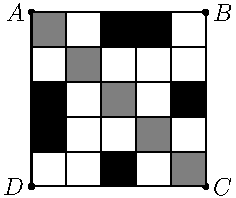
\includegraphics[scale=1.5]{Image/2017.pdf}
    \end{center}
        
        \item Cho $n=2017$. Hãy tìm giá trị nhỏ nhất của $k$ sao cho luôn có một cách gán số $k$-cân đối cho một cách tô màu đối xứng.
\end{enumerate}

    \end{btvn}

    \item \begin{btvn}\vocab{(Vietnam TST 2017).} Có $44$ lỗ khác nhau trên một đường thẳng và $2017$ con kiến. Mỗi con kiến bò ra khỏi một lỗ và bò dọc theo đường thẳng với tốc độ không đổi vào một lỗ khác, sau đó lại vào. Đặt $T$ là tập hợp các khoảnh khắc mà con kiến ra hoặc vào lỗ. Cho biết rằng $|T|\leq 45$ và tốc độ của các con kiến là khác nhau. Chứng minh rằng tồn tại ít nhất hai con kiến không va chạm nhau.
    \end{btvn}


    \item \begin{btvn}\vocab{(VMO 2018).}
        Một nhà đầu tư có hai mảnh đất hình chữ nhật có kích thước $120\times 100$.
        \begin{enumerate}[label=(\alph*)]
            \item Trên mảnh đất thứ nhất, cô ấy muốn xây dựng một ngôi nhà có mặt cắt hình chữ nhật kích thước $25\times 35$ và chín chậu hoa tròn với đường kính $5$ bên ngoài ngôi nhà. Chứng minh rằng ngay cả khi vị trí các chậu hoa được chọn ngẫu nhiên trên mảnh đất, diện tích còn lại vẫn đủ để xây dựng ngôi nhà như mong muốn.
            \item Trên mảnh đất thứ hai, cô ấy muốn xây dựng một ao cá đa giác sao cho khoảng cách từ một điểm tùy ý trên mảnh đất, bên ngoài ao cá, đến mép ao gần nhất không quá $5$. Chứng minh rằng chu vi của ao cá không nhỏ hơn $440-20\sqrt{2}$.
        \end{enumerate}
    \end{btvn}

   
    \item \begin{btvn}\vocab{(Vietnam TST 2018).}
        Đối với mỗi số nguyên dương $m$, một hình chữ nhật có kích thước $m\times 2018$ gồm các ô đơn vị được gọi là ''\textit{hoàn chỉnh}'' nếu các điều kiện sau được thỏa mãn:
        \begin{enumerate}
            \item Trong mỗi ô được viết một số "$0$", một số "$1$" hoặc không gì cả
            \item Đối với mọi chuỗi nhị phân $S$ có độ dài $2018$, ta có thể chọn một hàng và điền vào các ô trống sao cho các số trong hàng đó, nếu đọc từ trái sang phải, tạo ra $S$ (trong trường hợp đặc biệt, nếu một hàng đã đầy và tạo ra $S$ theo cùng một cách thức thì điều kiện ii. này được thỏa mãn).
        \end{enumerate}
        Một hình chữ nhật \textit{hoàn chỉnh} được gọi là \textit{tối thiểu}, nếu ta loại bỏ bất kỳ hàng nào của nó và sau đó nó không còn hoàn chỉnh nữa.
        \begin{enumerate}[label=(\alph*)]
        \item Chứng minh rằng đối với mọi số nguyên dương $k\le 2018$, tồn tại một hình chữ nhật \textit{tối thiểu} có kích thước $2^k\times 2018$ với đúng $k$ cột chứa cả $0$ và $1$.
        \item Một hình chữ nhật \textit{tối thiểu} có kích thước $m\times 2018$ có đúng $k$ cột chứa ít nhất một số $0$ hoặc $1$ và các cột còn lại là trống. Chứng minh rằng $m\le 2^k$.
        \end{enumerate}
    \end{btvn}

    \item \begin{btvn}\vocab{(Vietnam TST 2018).} Trong một lưới vuông $m\times n$, với góc trên bên trái là $A$, có một tuyến đường đi dọc theo cạnh của lưới bắt đầu từ $A$ và ghé qua tất cả các điểm đơn lát (gọi là "nút") đúng một lần và kết thúc cũng tại $A$.
        \begin{enumerate}[label=(\alph*)]
            \item Chứng minh rằng tuyến đường này tồn tại nếu và chỉ nếu ít nhất một trong số $m, n$ là số lẻ.
            \item Nếu một tuyến đường như vậy tồn tại, thì số lượng điểm xoáy ít nhất là bao nhiêu?    
        \end{enumerate}
Một điểm xoáy là một nút khác với $A$ và nếu hai cạnh trên tuyến đường giao nhau tại nút đó là vuông góc.
    \end{btvn}

    \begin{bt}\vocab{(VMO 2019).} 
    Có một số tờ giấy kích thước $5\times 5$ với hai mặt được chia thành các ô vuông đơn vị cho cả hai mặt. Mỗi ô trên tờ giấy được sơn bằng một trong $n$ màu sắc, mỗi màu được sử dụng cho một ô, sao cho hai ô ở cùng vị trí trên hai mặt được sơn bằng cùng một màu. Hai tờ giấy được sơn được coi là giống nhau nếu màu của hai ô tương ứng giống nhau. Chứng minh rằng không có nhiều hơn
    \[
        \frac{1}{8}\left(n^{25}+ 4n^{15} + n^{13} + 2n^7\right)
    \]
    mảnh giấy màu đôi một không giống nhau.
    \end{bt}
        \begin{sol}
            
            Ta có thể hiểu bài toán là đếm số cách tô một tờ giấy $5 \times 5$ bởi $n$ màu sao cho khác nhau qua các phép quay và lật ngược. Thật vậy, ta có thể dùng ý tưởng của bổ đề Burnside để loại bỏ những cấu hình lặp lại. Tuy nhiên, khó khăn ở đây là nếu ta đếm thống thường (quy tắc nhân) rồi dùng Burnside thì có một vấn đề là có những cấu hình bị lặp ít hơn những cấu hình khác. Khi đó, ta phải chia từng trường hợp nhỏ để kiểm soát và cân bằng số lần lặp của từng cấu hình.
            
            Ở đây ta có thể đếm theo quỹ đạo là $D_8$, tức là mỗi cấu hình sẽ lặp lại (tối đa) 8 lần.

            Theo lý thuyết quỹ đạo của khối nhị diện, ta có các trường hợp đếm lặp là $2^3,2^2,2^1,2^2$ lần và quy ước các trường hợp lớn hơn kế thừa số trường hợp nhỏ hơn (tức là nếu lặp $4$ lần cũng có nghĩa là lặp $1$ và $2$ lần).

            \vocabh{Trường hợp 1:} Tổng quát. Theo quy tắc nhân thì ta có $n^{25}$ cách. Gọi những cấu hình ở trường hợp này là $\mathcal{T}$

            Với mỗi cấu hình có khả năng lặp ở $\mathcal{T}$ phải là một cách tô đối xứng. Ta có tổng cộng ba loại đối xứng: theo trục đứng (ngang), trục đường chéo, theo tâm như hình bên dưới, các trục là đường màu đỏ.

           
            Gọi $\mathcal{A},\mathcal{B},\mathcal{C}$ lần lượt là các cách tô màu đối xứng theo trục đứng, đường chéo và tâm.
            \begin{center}
                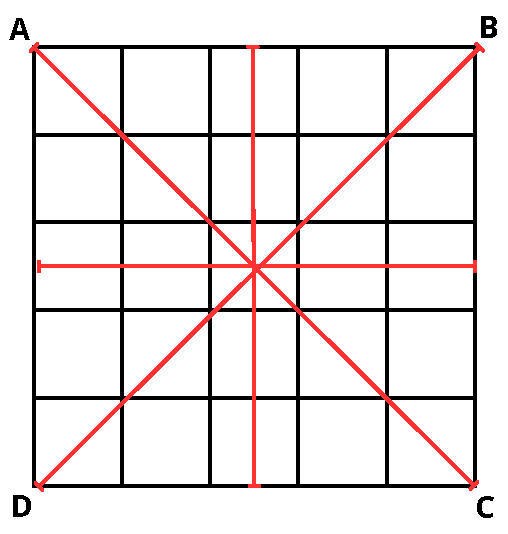
\includegraphics[scale=0.57]{Image/ex1.pdf}
            \end{center}
            \vocabh{Trường hợp 2: }Xét các cấu hình được đếm $4$ lần ở $\mathcal{T}$, khi đó những cấu hình này phải là $\mathcal{A}$ hoặc $\mathcal{B}$. Ví dụ như với trục ngang thì ta có thể tô trục bằng $5$ màu và mỗi bên bằng $10$ màu, tức là cần $15$ màu (có thể trùng nhau).
            \begin{center}
                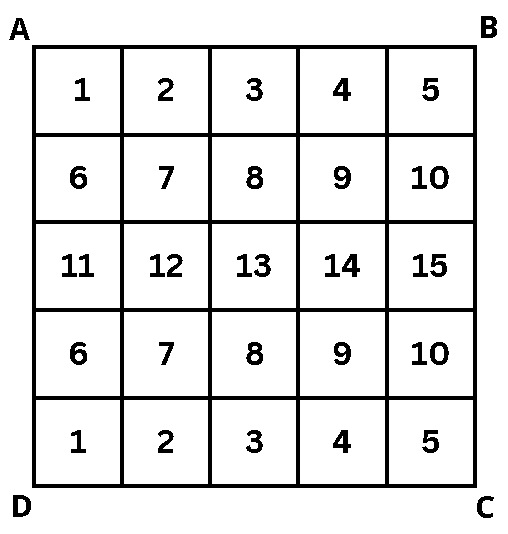
\includegraphics[scale=0.57]{Image/trucngang.pdf}
            \end{center}
            Đối với trục đứng thì bản chất là quay $90^{\circ}$ nên ta được $|\mathcal{A}| = 2n^{15}$. Mặt khác, rõ ràng $f: \mathcal{A} \to \mathcal{B}$ là một song ánh, khi ta cho các số nằm trên trục ngang hoặc dọc lên đường chéo, và mỗi bên đều chứa 10 số, tức là qua phép quay $45^{\circ}$ và ngược lại. Khi đó ta được $|\mathcal{A}|_{TH2} + |\mathcal{B}|_{TH2} = 4n^{15}$.

            \vocabh{Trường hợp 3: }Xét các cấu hình được đếm $2$ lần ở $\mathcal{T}$. Khi này một cách đếm thỏa mãn là bao hàm những cấu hình đối xứng qua cả hai trục ngang-dọc hoặc $AC$-$BD$. Tiến hành tương tự, ta chỉ có thể tô hai trục bằng $3$ màu. Khi đó sẽ chia thành $4$ phần $2\times2$, tô $4$ ô này bằng $4$ màu khác nhau. Ta được tổng cộng $7$ màu. Tương tự cho trục chéo, ta được $|\mathcal{A}|_{TH3} + |\mathcal{B}|_{TH3} = 2n^{7}$.
            \begin{center}
                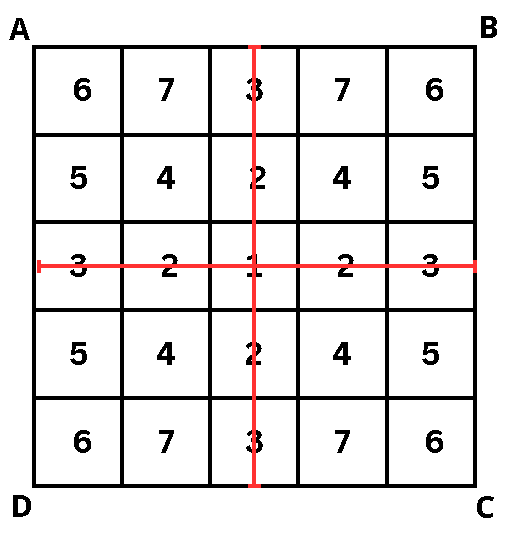
\includegraphics[scale=0.57]{Image/+.pdf}
            \end{center}
            \vocabh{Trường hợp 4: }Xét các cấu hình chỉ lặp lại 1 lần trong $\mathcal{T}$ và cả các kiểu đối xứng không phải trục. Rõ ràng ta phải tính $|\mathcal{C}|$ vì $\mathcal{A} \cap \mathcal{B} \subset \mathcal{C}$. Thật vậy, chọn ô giữa làm tâm, thì khi đó ta được $12$ cặp điểm và ảnh đối xứng của nó, tức là có thể dùng $13$ màu bất kì, ta được $|\mathcal{C}| = n^{13}$.
            \begin{center}
                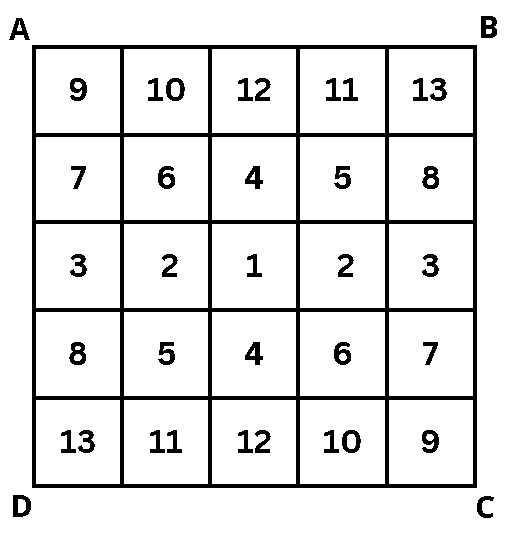
\includegraphics[scale=0.57]{Image/tam.pdf}
            \end{center}

            Cộng tất cả các trường hợp trên lại và áp dụng bổ đề Burnside, ta được tổng số các tô không đối xứng là 
            \[
            S = \frac{1}{8} \left(n^{25} + 4n^{15} + n^{13} + 2n^7\right)
            \]
        \end{sol}
    \begin{bt}\vocab{(Vietnam TST 2019).} Trong một quốc gia có $n\geq 2$ thành phố. Bất kỳ hai thành phố nào cũng có đúng một đường hàng không hai chiều. Chính phủ muốn cấp giấy phép cho một số hãng hàng không để chịu trách nhiệm với các đường hàng không này với các điều kiện sau:
        \begin{enumerate}
            \item Mỗi đường hàng không chỉ có thể được cấp giấy phép cho đúng một hãng hàng không.
            \item Bằng cách chọn một hãng hàng không bất kỳ, chúng ta có thể di chuyển từ một thành phố đến bất kỳ thành phố nào khác, chỉ sử dụng các chuyến bay từ hãng hàng không này.
        \end{enumerate}
        Số lượng tối đa các hãng hàng không mà chính phủ có thể cấp giấy phép để đáp ứng tất cả các điều kiện này là bao nhiêu?
    \end{bt}
    \begin{sol}
        Gọi $k$ là số hãng của quốc gia đó. Xét $K_n = (V,E)$ có $n$ đỉnh, mỗi đỉnh là một thành phố, đôi một kề nhau. Nếu thành phố $u$ và $v$ kề nhau bởi hãng $a$ thì ta gán nhãn $a$ cho $uv$. Ta sẽ dự đoán giá trị lớn nhất của $k$.


        Để ý rằng một chu trình  đi qua hết tất cả các đỉnh thì có độ dài nhỏ nhất là $n - 1$, nếu mỗi nhãn được gán vào một chu trình dài $n-1$ thì có 
        $$
        k \leq \frac{\displaystyle \binom{n}{2}}{n-1} = \frac{n}{2}
        $$
        Ta sẽ chứng minh rằng có nhiều nhất $\left\lfloor\frac{n}{2}\right\rfloor$ nhãn trong $K_{2m}$ bằng quy nạp.\\
        \vocab{- Trường hợp 1: } $n = 2m$.\\
        Với $m = 1$ thì dễ dàng kiểm tra mệnh đề trên đúng.\\
        Mệnh đề quy nạp: Với $K_{2m}$ có $2m$ đỉnh$(m \geq 1)$ thì có tối đa $m$ nhãn.\\
        Xét đồ thị $K_{2m+2}$ có $2m + 2$ đỉnh. Thêm 2 đỉnh mới, gọi 2 đỉnh đó là $u$ và $v$, khi này mỗi đỉnh sẽ nhận vào $m$ nhãn từ các đỉnh thuộc $K_{2m}$. Nếu ta thêm 1 nhãn mới vào $m + 1$ cạnh còn lại của từng $u$ và $v$ thì hoàn tất bài toán.\\
        \vocab{- Trường hợp 2: } $n = 2m + 1$.\\
        Với $n = 2$ thì dễ dàng kiểm tra mệnh đề trên đúng.\\
        Mệnh đề quy nạp: Với $K_{2m + 1}$ có $2m + 1$ đỉnh$(m \geq 1)$ thì có tối đa $m$ nhãn.\\
        Xét đồ thị $K_{2m+3}$ có $2m + 3$ đỉnh. Thêm 2 đỉnh mới, gọi 2 đỉnh đó là $u$ và $v$, khi này mỗi đỉnh sẽ nhận vào $m$ nhãn từ các đỉnh thuộc $K_{2m+1}$. Nếu ta thêm 1 nhãn mới vào $m + 1$ cạnh còn lại của $u$ và $m + 2$ của $v$ hoặc ngược lại thì hoàn tất bài toán.\\
    \end{sol}
    \begin{bt}\vocab{(VMO 2020).}
        Cho một số nguyên dương $n>1$. Đặt $T$ là một tập chứa tất cả các tập hợp có thứ tự $(x;y;z)$ sao cho $x,y,z$ đều là các số nguyên dương phân biệt và $1\leq x,y,z\leq 2n$. Ngoài ra, một tập $A$ chứa các tập hợp có thứ tự $(u;v)$ được gọi là "kết nối" với $T$ nếu với mọi $(x;y;z)\in T$ thì $\{(x;y),(x;z),(y;z)\} \cap A \neq \varnothing$.
        \begin{enumerate}[label=(\alph*)]
            \item Tìm số phần tử của tập $T$.
            \item Chứng minh rằng tồn tại một tập ''kết nối'' với $T$ có đúng $2n(n-1)$ phần tử.
            \item Chứng minh rằng mọi tập ''kết nối'' với $T$ có ít nhất $2n(n-1)$ phần tử.
        \end{enumerate}

    \end{bt}
    \begin{sol}
        Theo quy tắc chỉnh hợp thì $|T| = A_{2n}^3 = 2n(2n-1)(2n-2)$\\
        Ta sẽ tổng quát hóa bài toán. Xét $G=(V,E)$ có $2n$ dỉnh và các trường hợp riêng cho $(x,y)$ với $x > y$. Nếu $(x,y) \notin A$ thì ta có cạnh $xy$. Rõ ràng là $G$ không được tồn tại tam giác, vì nếu như có một tam giác $uvw$ thì ta có $\{(u,v),(u,w),(v,w)\} \cup A = \varnothing$ trái giả thuyết. Lý do mà ta phải gọi phần bù như vậy là để tránh chuyện ta ghép 3 cặp $(u,v,w)$ có $v < u < w$ chẳng hạn thì rõ ràng là các bộ đôi không bao giờ tạo thành tam giác được, vì sẽ có một cạnh bé thuộc $G$ và một cạnh lớn không thuộc $G$. Cho nên theo định lý Mantel thì $|E(G)| \leq n^2$. Lấy phần bù của các cặp thì ta được số tập $(x,y) \in A$ là 
        $$
        \binom{2n}{2} - n^2 = n(2n - 1) - n^2 = n^2 -n
        $$
        Chứng minh tương tự với $x < y$ thì ta sẽ có được $|A| \geq 2n(n-1)$.\\
        Dấu bằng xảy ra khi và chỉ khi $G$  là đồ thị lưỡng phân $K_{n,n}$. Khi này ta chọn $A = \{(x,y) | 1\leq x \leq n, n + 1\leq y \leq 2n\}$ với $x$ và $y$ có thể đổi vị trí cho nhau. Khi ấy $|A| = 2n(n-1)$
    \end{sol}
    \begin{btvn}\vocab{(Vietnam TST 2020).}
    Cho $n$ là một số nguyên dương, có $4n$ đội tham gia một giải bóng đá. Trong mỗi vòng đấu, chúng ta sẽ chia $4n$ đội thành $2n$ cặp, và mỗi cặp đội sẽ thi đấu cùng một lúc. Sau giải đấu, được biết rằng mỗi cặp đội đã thi đấu tối đa một trận. Tìm số nguyên dương nhỏ nhất $a$, sao cho chúng ta có thể sắp xếp một lịch thi đấu thỏa mãn các điều kiện trên, và nếu chúng ta thêm một vòng đấu nữa, luôn có một cặp đội đã thi đấu trận đấu.
    \end{btvn}

    \item \begin{btvn}\vocab{(Vietnam TST 2020).} Hãy giả sử $n$ là một số nguyên dương. Trên một bảng có kích thước $(2n+1)\times (2n+1)$, mỗi ô được tô màu trắng hoặc đen. Trong mỗi hàng và mỗi cột, nếu số lượng ô màu trắng nhỏ hơn số lượng ô màu đen, chúng ta sẽ đánh dấu tất cả các ô màu trắng. Nếu số lượng ô màu trắng lớn hơn số lượng ô màu đen, chúng ta sẽ đánh dấu tất cả các ô màu đen. Đặt $a$ là số lượng ô màu đen, và $b$ là số lượng ô màu trắng, $c$ là số lượng ô được đánh dấu.

        Ví dụ đối với bảng $3\times 3$, $a=3$, $b=6$, $c=4$.
        \begin{center}
            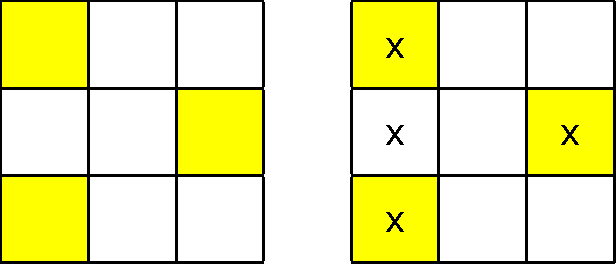
\includegraphics[scale=0.5]{Image/x.pdf}
        \end{center}
        Chứng minh rằng bất kể tình huống tô màu ban đầu như thế nào, luôn có $c\geq\frac{1}{2}\min\{a,b\}$.
    \end{btvn}

    \item \begin{btvn}\vocab{(VMO 2021).}
    Một học sinh chia tất cả $30$ viên bi vào $5$ hộp được đánh số $1, 2, 3, 4, 5$ (sau khi được chia, có thể có một hộp không có viên bi).
    \begin{enumerate}[label=(\alph*)]
        \item Có bao nhiêu cách để chia các viên bi vào các hộp (các cách chia khác nhau nếu có một hộp có số bi khác nhau)?
        \item Sau khi chia, học sinh sẽ sơn các viên bi đó bằng một số màu (mỗi màu sơn được cho nhiều viên bi, một màu có thể được sơn cho nhiều viên bi), sao cho không có $2$ viên bi trong cùng một hộp có màu giống nhau và từ bất kỳ $2$ hộp nào cũng không thể chọn $8$ viên bi đã được sơn bằng $4$ màu. Chứng minh rằng đối với mỗi cách chia, học sinh phải sử dụng ít nhất $10$ màu để sơn các viên bi.
        \item Hãy chỉ ra một cách chia sao cho với chính xác $10$ màu, học sinh có thể sơn các viên bi sao cho thỏa mãn các điều kiện trong câu b).
    \end{enumerate}
    \end{btvn}

    \item \begin{btvn}\vocab{(Vietnam TST 2021).} Trên một bảng gồm $2021 \times 2021$ ô vuông, chọn ra $k$ ô vuông đơn vị sao cho mỗi ô vuông được chọn có chung đỉnh với tối đa $1$ ô vuông khác được chọn. Xác định giá trị lớn nhất của $k$.
    \end{btvn}

    \item \begin{btvn}\vocab{(VMO 2022).}
        Cho 4 viên xúc xắc đồng chất. Ký hiệu $x_i (1\le x_i \le 6)$ là số chấm trên một mặt xuất hiện trên viên xúc xắc thứ $i$ $(1\le i \le 4)$.
        \begin{enumerate}[label=(\alph*)]
            \item Tìm các bộ số $(x_1,x_2,x_3,x_4)$
            \item Tìm xác suất để có một số $x_j$ sao cho $x_j$ bằng tổng của 3 số còn lại.
            \item Tìm xác suất để chúng ta có thể chia $x_1,x_2,x_3,x_4$ thành 2 nhóm có tổng bằng nhau.
        \end{enumerate}
    \end{btvn}

    \item \begin{btvn}\vocab{(Vietnam TST 2022).} Cho một đa diện lồi có 2022 mặt. Trong 3 mặt bất kỳ, đã có các số là $26$, $4$ và $2022$ (mỗi mặt chứa 1 số). Người ta muốn điền vào mỗi mặt còn lại một số thực là trung bình cộng của các số trong các mặt có cạnh chung với mặt đó. Chứng minh rằng chỉ có một cách để điền tất cả các số trong đa diện đó.
    \end{btvn}

    \item \begin{btvn}\vocab{(Vietnam TST 2022).} Cho một tập hợp $A=\{1;2;...;4044\}$. Người ta tô màu $2022$ số trong đó bằng màu trắng và các số còn lại bằng màu đen. Với mỗi $i\in A$, gọi số quan trọng của $i$ là số lượng tất cả các số trắng nhỏ hơn $i$ và các số đen lớn hơn $i$. Với mọi số tự nhiên $m$, hãy tìm tất cả các số nguyên dương $k$ mà tồn tại một cách tô màu các số sao cho có được $k$ số quan trọng bằng $m$.

    \end{btvn}

    \item \begin{btvn}\vocab{(VMO 2023).}
        Có $n \geq 2$ lớp học được tổ chức thành $m \geq 1$ nhóm ngoại khóa cho sinh viên. Mỗi lớp học có sinh viên tham gia ít nhất một nhóm ngoại khóa. Mỗi nhóm ngoại khóa có chính xác $a$ lớp mà các sinh viên trong nhóm này tham gia. Đối với bất kỳ hai nhóm ngoại khóa nào, không có nhiều hơn $b$ lớp với sinh viên tham gia cả hai nhóm đồng thời.
        \begin{enumerate}[label=(\alph*)]
            \item Tìm $m$ khi $n = 8, a = 4 , b = 1$.
            \item Chứng minh rằng $n \geq 20$ khi $m = 6 , a = 10 , b = 4$.
            \item Tìm giá trị nhỏ nhất của $n$ khi $m = 20 , a = 4 , b = 1$.
        \end{enumerate}
    \end{btvn}

    \item \begin{btvn}\vocab{(Vietnam TST 2023).}
    Một trường học có hai lớp học $A$ và $B$ lần lượt có $m$ và $n$ học sinh. Các học sinh của hai lớp học ngồi thành một vòng tròn. Sau đó, mỗi học sinh được tặng một số kẹo bằng số học sinh liên tiếp ngồi bên trái của anh ta đến từ lớp của anh ta. Sau khi phân phát kẹo, giáo viên quyết định nhóm các học sinh sao cho trong mỗi nhóm, tất cả các học sinh nhận được cùng một số lượng kẹo, và bất kỳ hai học sinh nào từ hai nhóm khác nhau đều phải nhận số lượng kẹo khác nhau.
    \begin{enumerate}[label=(\alph*)]
        \item Số học sinh tối đa mà một nhóm có thể có là bao nhiêu?
        \item Loại trừ nhóm mà mỗi học sinh không nhận được kẹo, số học sinh tối đa mà một nhóm có thể có là bao nhiêu?
    \end{enumerate}
    \end{btvn}

    \item \begin{btvn}\vocab{(Vietnam TST 2023).} Cho $n \geq 3$ là một số nguyên và $S$ là một tập hợp gồm $n$ phần tử. Xác định số nguyên lớn nhất $k_n$ sao cho: đối với mỗi cách chọn $k_n$ $3-$phần tử của $S$, tồn tại một cách tô màu các phần tử của $S$ bằng hai màu sao cho không có phần tử nào trong các $3-$phần tử được chọn là đơn sắc.
    \end{btvn}

    \item\begin{btvn}\vocab{(VMO 2024).}
    Cho $k$ viên bi được đặt lên các ô của một lưới $2024 \times 2024$ sao cho mỗi ô có tối đa một viên bi và không có hai viên bi nào được đặt trên hai ô kề nhau (hai ô kề nhau được xác định là các ô có cạnh chung).
    \begin{enumerate}[label=(\alph*)]
        \item Giả sử $k=2024$. Tìm cách đặt các viên bi sao cho mỗi ô có tối đa một viên bi và không có hai viên bi nào được đặt trên hai ô kề nhau (hai ô kề nhau được xác định là các ô có cạnh chung).
        \item Xác định giá trị lớn nhất của $k$ sao cho đối với tất cả các sắp xếp của $k$ viên bi thỏa mãn các điều kiện trên, chúng ta có thể di chuyển một trong những viên bi đã đặt lên một trong các ô kề cạnh của nó và sắp xếp mới vẫn thỏa mãn các điều kiện trên.
    \end{enumerate}
    \end{btvn}

    \begin{bt}\vocab{(VMO 2024).}
        Trong không gian, có một đa diện lồi $D$ sao cho đối với mỗi đỉnh của $D$, có một số lẻ cạnh đi qua đỉnh đó. Chúng ta chọn một mặt $F$ của $D$ sau đó gán mỗi cạnh của $D$ một số nguyên dương sao cho đối với tất cả các mặt của $D$ khác với $F$, tổng các số được gán trên các cạnh của mặt đó là một số nguyên dương chia hết cho $2024$. Chứng minh rằng tổng các số được gán trên các cạnh của $F$ cũng là một số nguyên dương chia hết cho $2024$.
    \end{bt}
    \begin{sol}
        \textbf{\vocab{Bình luận: }}\textit{Đối với các bài toán hình học tổ hợp, đặc biệt là đa diện trong không gian, ý tưởng quen thuộc là ta luôn có thể đưa bài toán về chứng minh đồ thị phẳng. Nguồn gốc của ý tưởng này là cách chứng minh công thức về số cạnh, đỉnh và mặt đa diện của Euler.\\
        Ta chọn một mặt đáy sau đó mở rộng mặt đáy này ra, các mặt khác của đa diện sẽ trở thành các miền trong mặt đáy, do các cạnh, đỉnh và miền vẫn được bảo toàn nên ta có thể đưa bài toán về đồ thị, với mặt đáy là $F$. Ta có hình minh họa như sau.}
    
    
    
            \begin{center}
                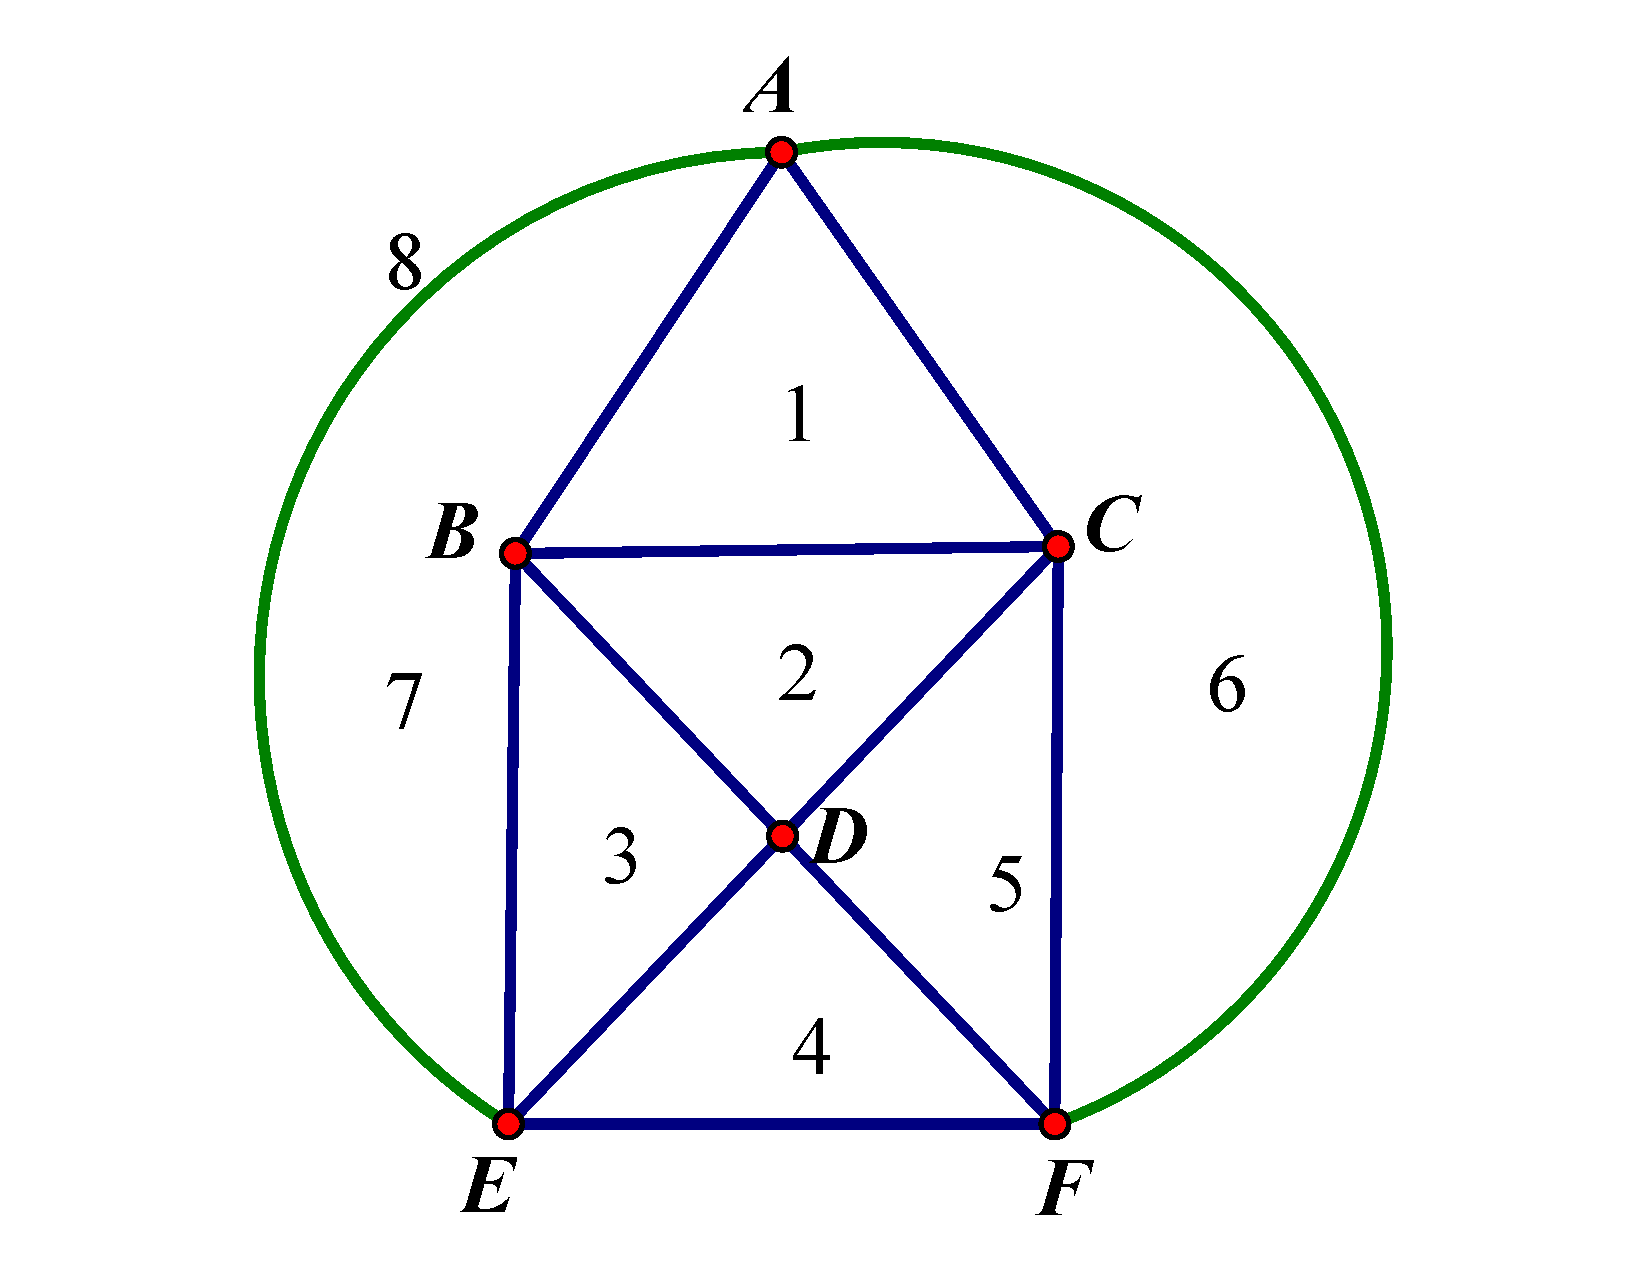
\includegraphics[scale=0.24]{Image/7.pdf}
            \end{center}

        Gọi đồ thị đang xét là $G(V,E)$. Từ giờ ta quy ước $w(u)$ là trọng số của cạnh $u$ và $sum(P)$ là tổng các $w(u)$ của miền $P$ và $2024 \mid sum(P)$ với mọi $P$.


        \textbf{\vocab{Bình luận: }}\textit{Ý tưởng chính của bài toán đồ thị này là ta cố gắng đưa về đồ thị phẳng lưỡng phân, khi đó bài toán dễ dàng chứng minh được khi ta chỉ cần so sánh số cạnh theo 2 cách. Tới đây tôi chợt nhớ ra trong quá khứ từng tồn tại một bài toán cực kì cổ điển là bài toán đi qua 7 cây cầu của Euler. Khi đó Euler chọn các vùng đất là đỉnh và cạnh là cây cầu của đồ thị. Vậy tại sao ta không làm điều tương tự đối với bài toán này?}\\
        Ta chọn các miền làm đỉnh của đồ thị mới, hai miền kề nhau được nối bởi 1 cạnh, khi đó đồ thị trở thành
        \begin{center}
            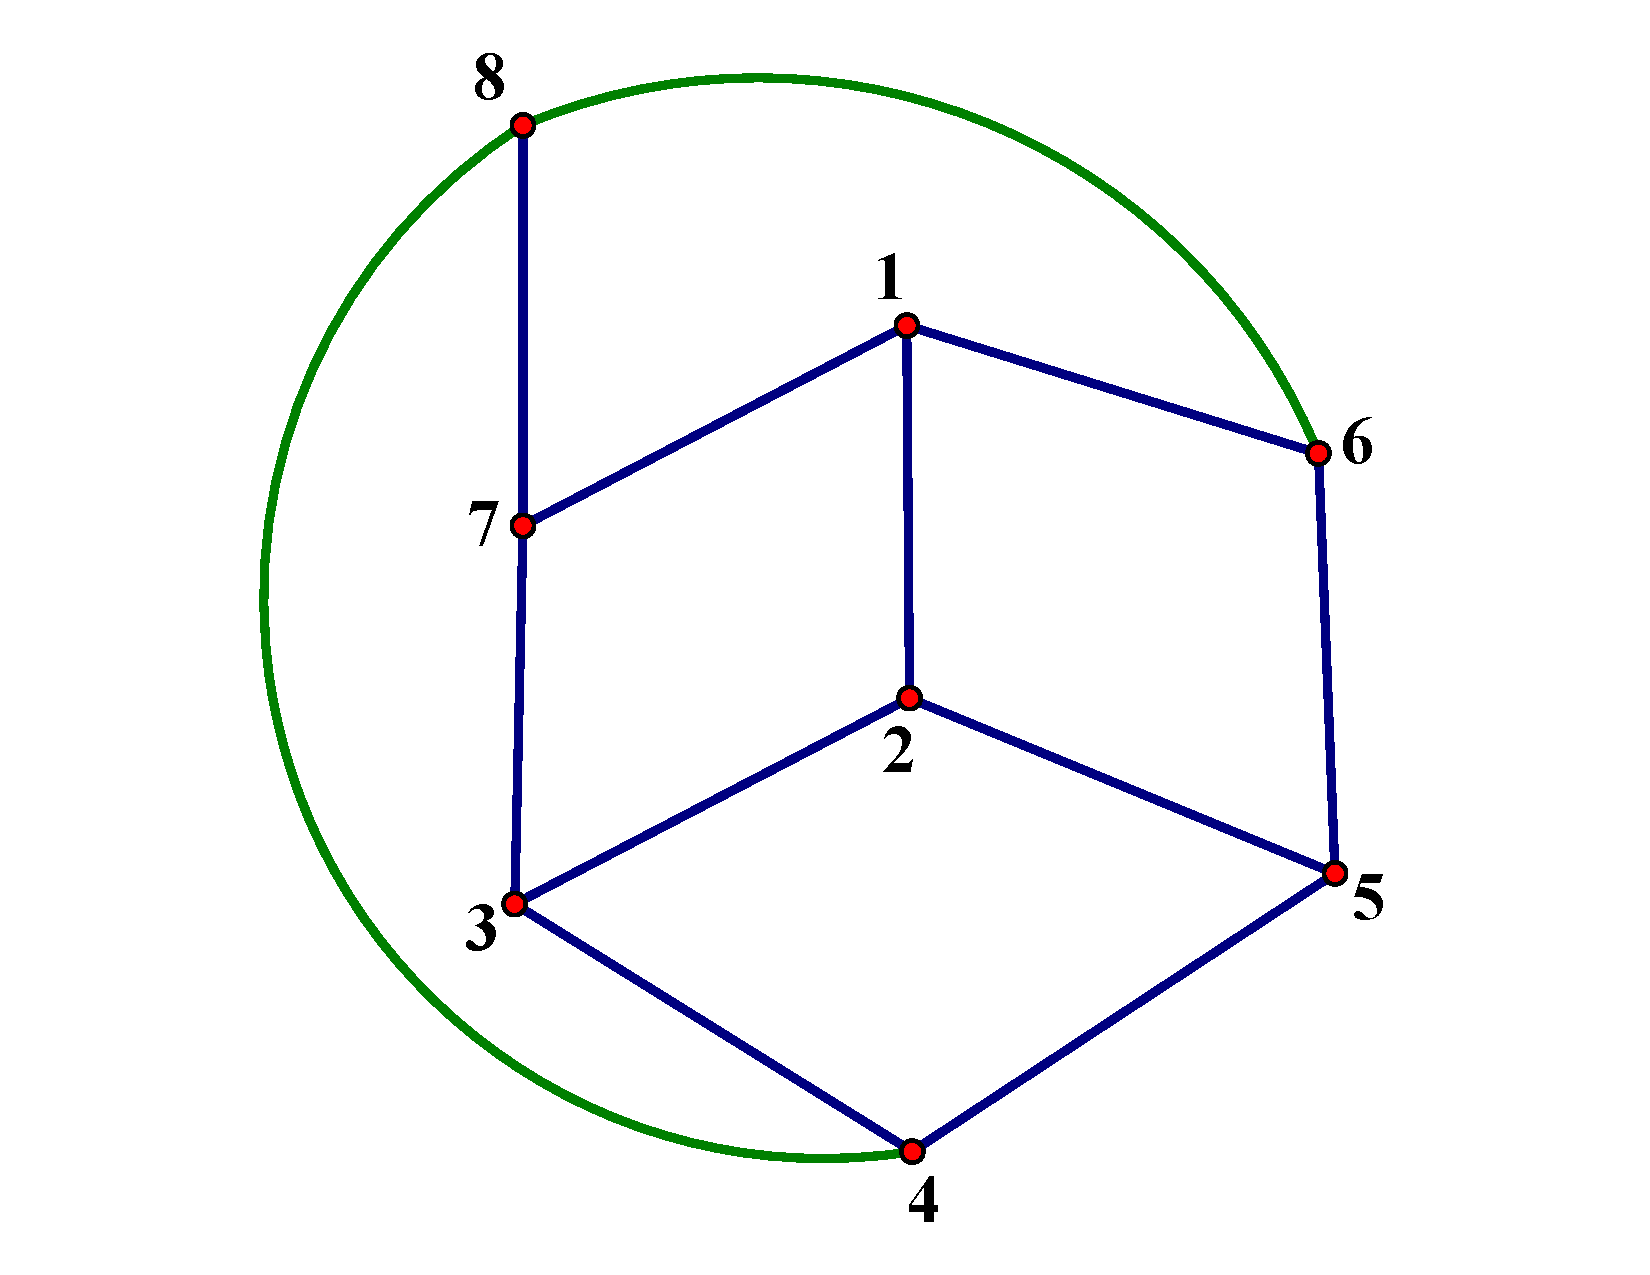
\includegraphics[scale=0.22]{Image/8.pdf}
        \end{center}
        Gọi đồ thị này là $G'(V',E')$. Việc chứng minh $G'$ là đồ thị phẳng cũng không khó, nếu ta vẽ các đỉnh tương ứng với vị trí của từng miền của $G$ thì rõ ràng $G'$ phẳng vì không có 2 miền nào được nối chéo nhau.\\
        Rõ ràng $f: G \to G'$ là song ánh nên không mất tính tổng quát ban đầu. Ta để ý rằng mỗi cạnh của $G'$ đều cắt duy nhất một cạnh của $G$ tương ứng ban đầu nên ta có có thể xem $v'$ là $v$. Và mỗi đỉnh của $G$ được bao bọc bởi các cạnh của $G'$ nên đỉnh trở thành miền. Tóm lại, ta được điều như sau:
        $$ f: G \to G', \text{cạnh} \mapsto \text{cạnh}, \text{đỉnh} \mapsto \text{miền}, \text{miền} \mapsto \text{đỉnh}
        $$
        Khi này,  $sum(P)$ có thể được hiểu là tổng $w(u)$ nằm trên cạnh chứa đỉnh $P$\\
        Tiếp theo ta cần chứng minh $G'$ lưỡng phân. Theo bổ đề Koenig, cần chứng minh các chu trình của $G'$ đều chẵn. Ta biết rằng mỗi miền của $G'$ đều được tạo bởi chẵn các cạnh. Thật vậy, ta xét một chu trình đi qua các cạnh của $F$. Khi này ta thu hẹp chu trình lại theo từng miền.\\
        Đặt độ dài ban đầu của chu trình bị thu hẹp là $x$, độ dài miền bất kì là $y$. Rõ ràng là ta có $2 \mid x + y$, hay $x \equiv y \pmod 2$ (vì ta bớt ra $y-1$ cạnh do miền chẵn và thêm vào 1 nên tính chẵn lẻ giữ nguyên). Mà $y$ chẵn nên $x$ chẵn. \\
        Cứ thu hẹp các chu trình liên tục như thế thì rõ ràng mọi chu trình đều chẵn. Theo bổ đề trên thì $G'$ lưỡng phân.


        \begin{center}
            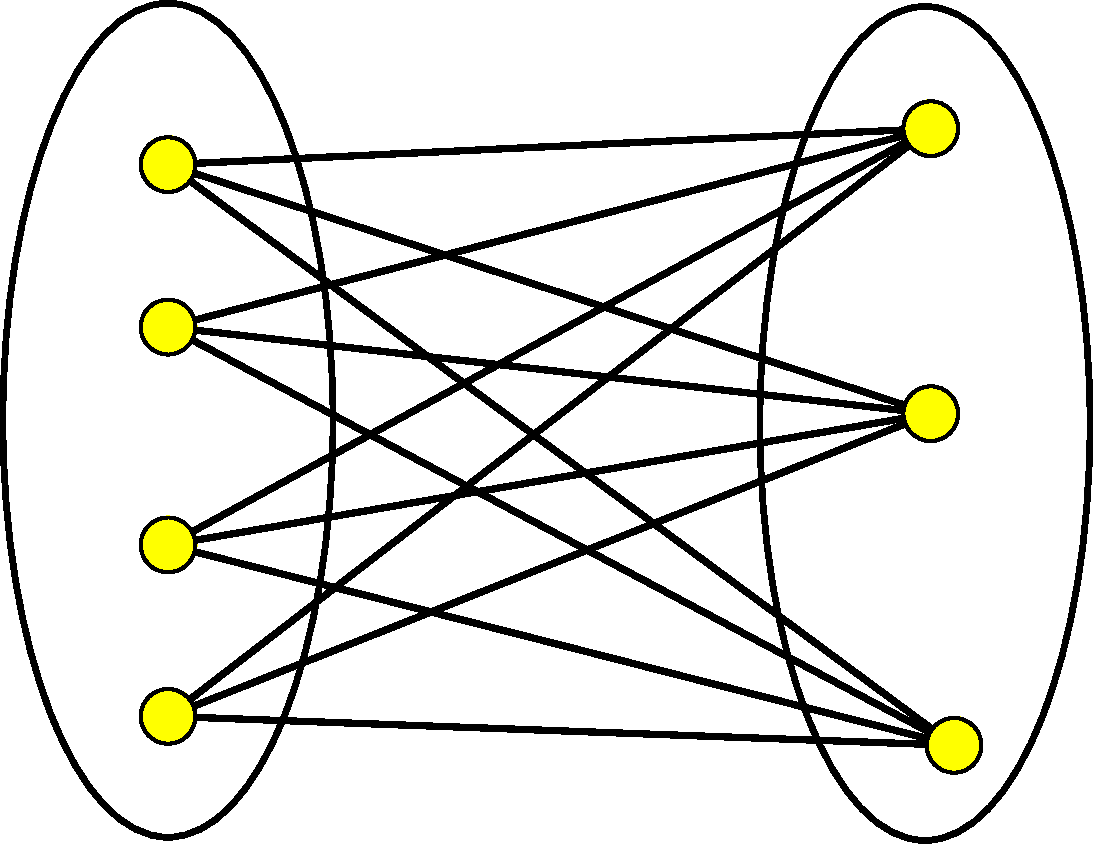
\includegraphics[scale=0.25]{Image/kphec.pdf}
        \end{center}
        Chia $G'$ thành 2 phe là phe $X$ có chứa $F$ và phe $Y$ không chứa $F$ như hình. Ta tiến hành đếm trọng số các cạnh theo hai cách.
        \begin{itemize}[label=]
            \item \vocab{Cách 1 (theo phe Y):}   Rõ ràng phe $Y$ không chứa $F$ nên ta luôn có $$\sum_{P \in Y} sum(P) = \sum_{A \in G'}sum(A) \text{ } \vdots \text{ }2024$$
            \item \vocab{Cách 2 (theo phe X):}  Ta có 
            $$\sum_{f \in F}sum(f) + \sum_{p \in X \notin F}sum(p) =  \sum_{A \in G'}sum(A) \text{ } \vdots \text{ }2024
            $$
        \end{itemize}
        Mặt khác, rõ ràng $\displaystyle  \sum_{p \in X \notin F}sum(p)\text{ } \vdots \text{ }2024$ nên do đó ta phải có $\displaystyle\sum_{f \in F}sum(f) \text{ } \vdots \text{ }2024$. Nói cách khác, tổng các trọng số của các cạnh chứa đỉnh $F$ phải chia hết cho 2024, mà khi ta quy về $G$ về đa diện, đỉnh $F$ trở thành miền $F$ thành mặt $F$ có tổng trọng số các cạnh chia hết cho 2024. Điều này cho ta điều phải chứng minh. 
    \end{sol}
    \begin{bt}\vocab{(Vietnam TST 2024).} Trong một khu vườn có các ô vuông $2024\times 2024$, người ta trồng ba loại hoa: hoa hồng, hoa cúc và hoa lan. Người ta muốn trồng hoa sao cho các điều kiện sau được thỏa mãn:
        \begin{enumerate}
            \item Mỗi ô được trồng tối đa một loại hoa. Một số ô có thể để trống và không trồng hoa.
            \item Đối với mỗi ô được trồng $A$, có đúng $3$ ô khác được trồng trong cùng một cột hoặc hàng sao cho ba ô đó được trồng với các loại hoa khác nhau so với ô $A$.
            \item Mỗi loại hoa được trồng ít nhất trong $1$ ô.
        \end{enumerate}
        Số lớn nhất của các ô có thể được trồng hoa là bao nhiêu?
    \end{bt}
    \begin{sol}
        Gọi $u,v,w$ là nhãn cúc, hồng, lan. Và ta sẽ tìm cách gán nhiều nhãn $u,v,w$ nhất đồng thời thỏa mãn các điều kiện bài toán.
        Ta sẽ \pf{divide and conquer} bài toán này để dễ xử lý hơn. Không mất tính tổng quát, ta xét một hàng bất kì (làm tương tự với cột). Rõ ràng sẽ có 3 khả năng xảy ra đối với các ô: có 1 nhãn duy nhất, có 2 nhãn khác nhau, có 3 nhãn khác nhau. Trường hợp tầm thường là không có nhãn nào hết thì ta không để ý đến.
        \begin{itemize}
            \item \vocab{Trường hợp 1: chỉ có 1 nhãn duy nhất}. Rõ ràng là bất kì một cột nào giao với 1 ô thuộc hàng này cũng chỉ chứa đúng 1 nhãn duy nhất.
            \item \vocab{Trường hợp 2: có 2 nhãn khác nhau}. Ta thấy rằng là hàng này chỉ có thể chứa tối đa 6 ô dán nhãn, vì nếu không, theo nguyên lý Dirichlet, tồn tại một nhãn được dán 4 lần, mâu thuẫn điều 3.
            \item \vocab{Trường hợp 3: có 3 nhãn khác nhau}. Tương tự với trường hợp 2, ta cũng biết được hàng này chỉ có thể chứa tối đa 6 ô dán nhãn.
        \end{itemize}
        Ta gọi trường hợp 1 là loại cách dán $A$, trường hợp 2 và 3 là cách dán loại $B$ và chúng cũng tương tự nhau.


        Bản chất của bài toán này là yêu cầu đi tìm cách dán nhãn nhiều nhất mà không quan tâm đến mỗi loại nhãn có bao nhiêu cái, nên ta chỉ cần chỉ ra một cách dán tối ưu là được.


        Nếu có tối đa $k$ hàng cũng dán cùng nhãn cùng loại $B$, ta có được hình chữ nhật $R_1 = 6\times k$. Thì ta sẽ có ít nhất $2024 - k$ hàng còn lại cùng dán loại $A$ và được hình chữ nhật $R_2 = (2024-k)\times(2024-6)$. Tuy nhiên, do hàng và cột là như nhau, nên nếu ta xoay $R_2$ lại thì rõ ràng để thỏa mãn điều 3 thì chiều dài của $R_2$ phải là một cách dãn nhãn loại $B$. Nói cách khác $2024 - k \leq 6$. Tương đương $k \geq 2018$. Vì vậy $R_1 + R_2 \leq 2018.6 + 6.2018 = 12.2018$. Và đây là một cách minh họa có kiểu dán nhãn đó.
        \begin{center}
            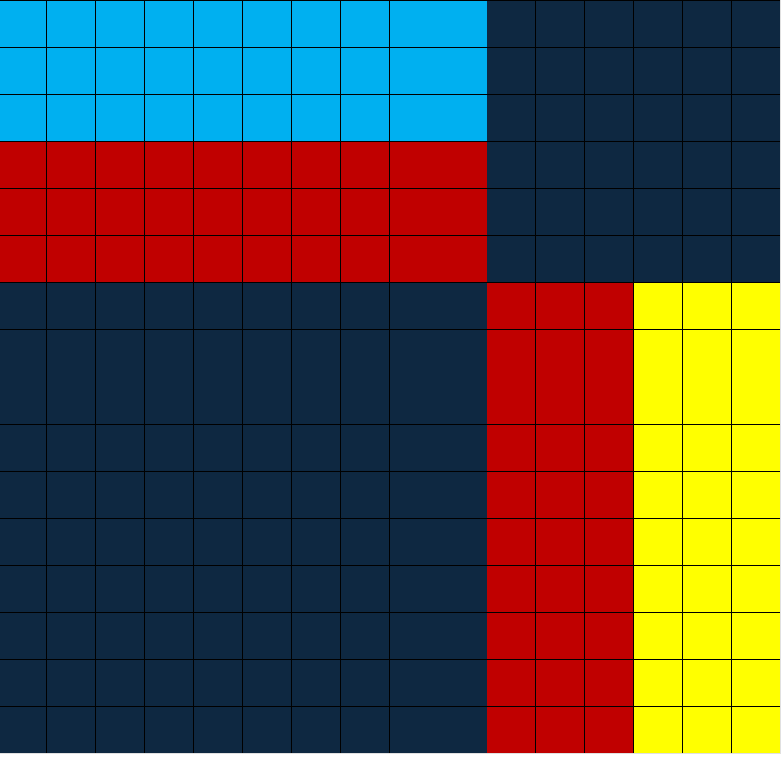
\includegraphics[scale=0.3]{Image/tst.pdf}
        \end{center}
        Tất nhiên các nhãn có thể chọn tùy ý, miễn có ít nhất 2 nhãn trở lên.
    \end{sol}
    \begin{btvn}\vocab{(IMO Shortlist 2010 C1).}
        Trong một buổi hòa nhạc, 20 ca sĩ sẽ biểu diễn. Đối với mỗi ca sĩ, có một nhóm (có thể trống) các ca sĩ khác để anh ấy muốn biểu diễn muộn hơn tất cả các ca sĩ từ bộ đó. Có thể xảy ra rằng có chính xác 2010 đơn đặt hàng của các ca sĩ để tất cả mong muốn của họ được thỏa mãn?
    \end{btvn}
    \begin{btvn}\vocab{(IMO Shortlist 2010 C2).}
        Trên một vài hành tinh, có $2^n$ quốc gia $(n \geq 4)$. Mỗi quốc gia có một lá cờ rộng $n$ đơn vị và cao một đơn vị gồm có $n$ ô vuông $1\times 1$, mỗi ô có thể có màu xanh hoặc vàng. Không có hai quốc gia nào có cùng lá cờ. Chúng ta nói rằng một tập hợp $n$ lá cờ là đa dạng nếu các lá cờ đó có thể sắp xếp thành $n \times n$ ô vuông sao cho $n$ ô vuông trên đường chéo chính có cùng màu. Xác định giá trị nhỏ nhất của $m$ sao cho mới mọi $m$ là cờ phân biệt, luôn tồn tại $n$ lá cờ tạo nên một tập đa dạng.
    \end{btvn}
     \begin{btvn}\vocab{(IMO Shortlist 2010 C3).}
        2500 quân vua được đặt trên bàn cờ $100 \times 100$ sao cho
        \begin{enumerate}
            \item Không vị vua nào có thể bắt được bất kỳ vị vua nào khác (tức là không có hai vị vua nào được đặt trong hai ô vuông có chung một đỉnh)
            \item Mỗi hàng và mỗi cột chứa chính xác 25 vị vua.
        \end{enumerate}
        Tìm số lượng sắp xếp như vậy. (Hai cách sắp xếp khác nhau bằng cách xoay hoặc đối xứng được cho là khác nhau.)

    \end{btvn}
    
     \begin{btvn}\vocab{(IMO/IMO Shortlist 2010 C4).}
        Mỗi hộp trong số sáu hộp $B_1$, $B_2$, $B_3$, $B_4$, $B_5$, $B_6$ ban đầu chứa một đồng xu. Ta có các hoạt động như sau:

        \begin{itemize}[label=-]
            \item \vocab{Loại 1:} Chọn một hộp không trống $B_j$, $1\leq j \leq 5$, loại bỏ một đồng xu khỏi $B_j$ và thêm hai đồng xu vào $B_{j+1}$;
            \item \vocab{Loại 2:} Chọn một hộp không trống $B_k$, $1\leq k \leq 4$, loại bỏ một đồng xu khỏi $B_k$ và hoán đổi số đồng xu (có thể trống) của các hộp $B_{k+1}$ và $ B_{k+2}$.

        \end{itemize}
        Xác định xem có tồn tại một chuỗi hữu hạn các phép toán thuộc các loại trên hay không, sao cho năm hộp $B_1$, $B_2$, $B_3$, $B_4$, $B_5$ trở nên trống rỗng, trong khi hộp $B_6$ chứa chính xác $2010^ {2010^{2010}}$ xu.
    \end{btvn}

   

    \item \begin{btvn}\vocab{(IMO Shortlist 2011 C1).} Cho $n > 0$ là một số nguyên. Chúng ta có một cái cân và $n$ quả cân trọng lượng $2^0, 2^1, \cdots, 2^{n-1}$. Chúng ta đặt từng quả cân lên cân sao cho đĩa bên phải không bao giờ nặng hơn đĩa bên trái. Ở mỗi bước, chúng ta chọn một trong các quả cân chưa được đặt lên cân và đặt nó lên đĩa bên trái hoặc đĩa bên phải cho đến khi tất cả các quả cân đã được đặt xong. Hãy xác định số cách có thể thực hiện được điều này.
    \end{btvn}

    \item \begin{btvn}\vocab{(IMO Shortlist 2011 C2).}
        Giả sử rằng sinh viên $1000$ đang đứng thành một vòng tròn. Chứng minh rằng tồn tại một số nguyên $k$ với $100 \leq k \leq 300$ sao cho trong vòng tròn này tồn tại một nhóm liền kề gồm $2k$ học sinh, trong đó nửa đầu chứa số nữ sinh bằng nửa sau.
    \end{btvn}



    \item \begin{btvn}\vocab{(IMO Shortlist 2011 C4).}
        Xác định số nguyên dương lớn nhất $k$ thỏa mãn tính chất sau: Tập hợp các số nguyên dương có thể được phân chia thành $k$ tập con $A_1, A_2, \ldots, A_k$ sao cho mọi số nguyên $n \geq 15$ và tất cả $i \in \{1, 2, \ldots, k\}$ tồn tại hai phần tử riêng biệt của $A_i$ có tổng là $n$.
    \end{btvn}

    \item \begin{btvn}\vocab{(IMO Shortlist 2012 C1).}
        Một vài số nguyên dương được viết thành một hàng. Liên tục lặp lại, Alice chọn hai số liền kề $x$ và $y$ sao cho $x>y$ và $x$ nằm ở bên trái của $y$, và thay thế cặp $(x,y)$ bằng $(y +1,x)$ hoặc $(x-1,x)$. Chứng minh rằng cô ấy chỉ có thể thực hiện hữu hạn nhiều lần lặp như vậy.
    \end{btvn}

    \item \begin{btvn}\vocab{(IMO Shortlist 2012 C2).}
        Cho $n \geq 1$ là một số nguyên. Số lượng tối đa các cặp phần tử rời nhau của tập $\{ 1,2,\ldots , n \}$ sao cho tổng của các cặp khác nhau là các số nguyên khác nhau không vượt quá $n$?
    \end{btvn}

    \item \begin{btvn}\vocab{(IMO Shortlist 2012 C3).}
    Trong một bảng vuông $999 \times 999$, một số ô có màu trắng và các ô còn lại có màu đỏ. Gọi $T$ là số bộ ba $(C_1,C_2,C_3)$ của các ô, hai ô đầu tiên trong cùng một hàng và hai ô cuối cùng trong cùng một cột, với $C_1,C_3$ màu trắng và $C_2$ màu đỏ. Tìm giá trị lớn nhất $T$ có thể đạt được.
    \end{btvn}


    \item \begin{btvn}\vocab{(IMO Shortlist 2012 C7).}
        Cho $2^{500}$ điểm nằm trên một đường tròn được đánh theo số thứ tự $1,2,\dots,2^{500}$. Chứng minh rằng có thể chọn ra $100$ cặp điểm rời nhau để nối một số điểm trong số này sao cho $100$ tổng của các cặp số tại điểm cuối của dây cung đã chọn là bằng nhau.
    \end{btvn}

    \item\begin{btvn}\vocab{(IMO Shortlist 2013 C1).} Cho $n$ là một số nguyên dương. Tìm số nguyên nhỏ nhất $k$ có tính chất sau; Cho bất kỳ số thực $a_1 , \cdots , a_d $ sao cho $a_1 + a_2 + \cdots + a_d = n$ và $0 \le a_i \le 1$ với $i=1,2,\cdots ,d$, nó có thể phân chia các số này thành các nhóm $k$ (một số có thể trống) sao cho tổng các số trong mỗi nhóm nhiều nhất là $1$.
    \end{btvn}
    
    \item \begin{btvn}\vocab{(IMO/IMO Shortlist 2013 C2).}
        Một cấu hình gồm các điểm $4027$ trong mặt phẳng được gọi là Colombia nếu nó bao gồm $2013$ điểm đỏ và $2014$ điểm xanh, và không có ba điểm nào trong cấu hình thẳng hàng. Bằng cách vẽ một số đường, mặt phẳng được chia thành nhiều vùng. Việc sắp xếp các đường là tốt cho cấu hình Colombia nếu hai điều kiện sau được thỏa mãn:
        \begin{enumerate}
            \item Không có đường thẳng nào đi qua bất kỳ điểm nào của hình.
            \item Không có vùng nào chứa điểm có cả hai màu.
        \end{enumerate}
        Tìm giá trị nhỏ nhất của $k$ sao cho với bất kỳ cấu hình Colombia nào có $4027$ điểm , có sự sắp xếp hợp lý cho $k$ đường thẳng.
    \end{btvn}
    

    \item \begin{btvn}\vocab{(IMO Shortlist 2014 C3).}
        Cho $n \ge 2$ là một số nguyên. Xét một bàn cờ vua $n \times n$ gồm $n^2$ ô đơn vị. Một cấu hình của $n$ quân xe trên bảng này là hòa bình nếu mỗi hàng và mỗi cột chứa đúng một quân xe. Tìm số nguyên dương lớn nhất $k$ sao cho, đối với mỗi cấu hình hòa bình của $n$ quân xe, tồn tại một ô vuông $k \times k$ không chứa quân xe trên bất kỳ ô đơn vị nào trong $k^2$ ô của nó.
    \end{btvn}


    \item \begin{btvn}\vocab{(IMO Shortlist 2015 C3).}
        Cho một tập hợp hữu hạn $A$ gồm các số nguyên dương, một phân hoạch của $A$ thành hai tập hợp không giao nhau và khác rỗng $A_1$ và $A_2$ được gọi là $\textit{tốt}$ nếu bội chung nhỏ nhất của các phần tử trong $A_1$ bằng với ước chung lớn nhất của các phần tử trong $A_2$. Tìm giá trị nhỏ nhất của $n$ sao cho tồn tại một tập hợp gồm $n$ số nguyên dương với chính xác $2015$ phân hoạch tốt.
    \end{btvn}

    \item \begin{btvn}\vocab{(IMO Shortlist 2015 C4).}
        Cho $n$ là một số nguyên dương. Hai người chơi $A$ và $B$ chơi một trò chơi trong đó họ lần lượt chọn các số nguyên dương $k \leq n$. Các quy tắc của trò chơi là:
        \begin{enumerate}
            \item Một người chơi không thể chọn một số đã được chọn bởi bất kỳ người chơi nào trong các lượt chơi trước đó.
            \item Một người chơi không thể chọn một số liền kề với bất kỳ số nào mà người chơi đã chọn trước đó trong các lượt chơi trước đó.
            \item Trò chơi hòa nếu tất cả các số đã được chọn; nếu không, người chơi không thể chọn được số nào nữa thì sẽ thua cuộc.
        \end{enumerate}
        Người chơi $A$ thực hiện lượt chơi đầu tiên. Xác định kết quả của trò chơi, giả sử cả hai người chơi sử dụng chiến lược tối ưu.
    \end{btvn}

    
    \item \begin{btvn}\vocab{(IMO Shortlist 2016 C2).}    
        Tìm tất cả các số nguyên dương $n$ sao cho tất cả các ước số dương của $n$ có thể được đặt vào các ô của một bảng hình chữ nhật dưới các ràng buộc sau:
        \begin{enumerate}
            \item Mỗi ô chứa một ước số khác nhau
            \item Tổng của tất cả các hàng bằng nhau
            \item Tổng của tất cả các cột bằng nhau.
        \end{enumerate}
            \end{btvn}
    \item\begin{btvn}\vocab{(IMO Shortlist 2016 C3).}
        Cho $n$ là một số nguyên dương nguyên tố với $6$. Người ta sơn các đỉnh của một đa giác đều $n$ đỉnh bằng ba màu sao cho có một số lẻ đỉnh mỗi màu. Chứng minh rằng tồn tại một tam giác cân có ba đỉnh có ba màu khác nhau.
    \end{btvn}


    \item \begin{btvn}\vocab{(IMO Shortlist 2016 C5).}
        Cho $n \geq 3$ là một số nguyên dương. Tìm số lượng đường chéo tối đa có thể chọn trong một đa giác đều $n$ đỉnh, sao cho không có hai đường chéo nào cắt nhau bên trong hoặc chúng vuông góc với nhau.
    \end{btvn}


    \item \begin{btvn}\vocab{(IMO Shortlist 2016 C8).}
        Cho $n$ là một số nguyên dương. Xác định số nguyên dương nhỏ nhất $k$ có tính chất sau: có thể đánh dấu $k$ ô trên một bảng $2n \times 2n$ sao cho tồn tại một phân chia duy nhất của bảng thành các ô vuông $1 \times 2$ và $2 \times 1$, không có ô nào chứa hai ô đã đánh dấu.
    \end{btvn}

    \item \begin{btvn}\vocab{(IMO Shortlist 2017 C1).}
        Một hình chữ nhật $\mathcal{R}$ với độ dài cạnh là số nguyên lẻ được chia thành các hình chữ nhật nhỏ có độ dài cạnh là số nguyên. Chứng minh rằng luôn tồn tại ít nhất một trong các hình chữ nhật nhỏ mà khoảng cách từ bốn cạnh của $\mathcal{R}$ đến hình chữ nhật nhỏ đó đều là số lẻ hoặc đều là số chẵn.
    \end{btvn}

    \item \begin{btvn}\vocab{(IMO Shortlist 2017 C2).}
        Cho $n$ là một số nguyên dương. Một chuỗi \textit{nhện} là một chuỗi bất kỳ gồm $3n$ chữ cái, với đúng $n$ lần xuất hiện của mỗi chữ cái $a, b,$ và $c$. Định nghĩa một hoán vị là sự hoán đổi của hai chữ cái liền kề trong một chuỗi nhện. Chứng minh rằng đối với bất kỳ chuỗi nhện $X$ nào, luôn tồn tại một chuỗi nhện $Y$ sao cho $X$ không thể được thay đổi thành $Y$ bằng ít hơn $3n^2/2$ lần hoán vị.
    \end{btvn}

    \item \begin{btvn}\vocab{(IMO Shortlist 2017 C3).}
        Sir Alex chơi trò chơi sau trên một hàng gồm 9 ô. Ban đầu, tất cả các ô đều trống. Trong mỗi lượt, Sir Alex được phép thực hiện chính xác một trong hai thao tác sau:
        \begin{enumerate}
            \item  Chọn bất kỳ số nào có dạng $2^j$, với $j$ là một số nguyên không âm, và đặt nó vào một ô trống.
            \item Chọn hai ô (không nhất thiết phải kề nhau) có cùng một số trong đó; gọi số đó là $2^j$. Thay thế số trong một ô bằng $2^{j+1}$ và xóa số trong ô kia.
            \item Cuối cùng, một ô chứa $2^n$, với $n$ là một số nguyên dương đã cho, trong khi các ô khác đều trống.
        \end{enumerate}
         Xác định số lượng lớn nhất các bước mà Sir Alex có thể đã thực hiện theo $n$.
    \end{btvn}

    \item \begin{btvn}\vocab{(IMO Shortlist 2017 C4).}
        Cho một số nguyên $N \ge 2$. Một tập hợp gồm $N(N + 1)$ cầu thủ bóng đá, không có hai người cùng chiều cao, đứng thành một hàng. Sir Alex muốn loại bỏ $N(N - 1)$ người từ hàng này, để lại một hàng mới gồm $2N$ người trong đó thỏa mãn $N$ điều kiện sau:

        (1) Không ai đứng giữa hai người cao nhất,

        (2) Không ai đứng giữa người thứ ba và người thứ tư cao nhất,

        $\;\;\vdots$

        (N) Không ai đứng giữa hai người thấp nhất.

        Chứng minh rằng điều này luôn có thể thực hiện được.
    \end{btvn}


    \item \begin{btvn}\vocab{(IMO Shortlist 2017 C5).}
        Tom và Jerry chơi một trò chơi trên một trục số. Điểm bắt đầu của Jerry - $A_0,$ và điểm bắt đầu của Tom - $B_0,$ là cùng một điểm. Sau $n-1$ lượt chơi, Jerry đang ở điểm $A_{n-1}$ và Tom ở điểm $B_{n-1}.$ Trong lượt chơi thứ $n$ của trò chơi, ba sự kiện xảy ra theo thứ tự:
        \begin{enumerate}
            \item Jerry di chuyển đến một điểm $A_n$ sao cho khoảng cách giữa $A_{n-1}$ và $A_n$ là chính xác $1$.
            \item Một thiết bị theo dõi báo cáo một điểm $P_n$ cho Tom. Đảm bảo duy nhất của thiết bị theo dõi với Tom là khoảng cách giữa $P_n$ và $A_n$ không vượt quá $1$.
            \item Tom di chuyển rõ ràng đến một điểm $B_n$ sao cho khoảng cách giữa $B_{n-1}$ và $B_n$ là chính xác $1$.
        \end{enumerate}
        Liệu có luôn luôn có thể, không phụ thuộc vào cách Jerrt di chuyển như thế nào và không phụ thuộc vào các điểm được báo cáo bởi thiết bị theo dõi, Tom có thể chọn cách di chuyển của mình sao cho sau $10^9$ lượt chơi, Tom có thể đảm bảo khoảng cách giữa Tom và Jerry không vượt quá $100?$
    \end{btvn}

    \item \begin{btvn}\vocab{(IMO Shortlist 2017 C6).}
        Cho số nguyên dương $n > 1$. Một khối lập phương $n \times n \times n$ được tạo thành từ $n^3$ khối lập phương đơn vị. Mỗi khối lập phương đơn vị được sơn bằng một màu. Đối với mỗi hộp $n \times n \times 1$ bao gồm $n^2$ khối lập phương đơn vị (trong bất kỳ ba hướng nào cũng được), chúng ta xem xét tập hợp các màu hiện diện trong hộp đó (mỗi màu chỉ được liệt kê một lần). Bằng cách này, chúng ta có được $3n$ tập hợp màu, được chia thành ba nhóm theo từng hướng.

        Đối với mỗi tập trong bất kỳ nhóm nào, cùng một tập xuất hiện trong cả hai nhóm còn lại. Xác định số lớn nhất có thể của các màu hiện diện theo $n$.
    \end{btvn}


    
    \item \begin{btvn}\vocab{(IMO Shortlist 2018 C1).}
        Cho số nguyên dương $n\geqslant 3$. Chứng minh rằng tồn tại một tập hợp $S$ gồm $2n$ số nguyên dương thoả mãn tính chất sau: Đối với mọi $m=2,3,...,n$ tập hợp $S$ có thể được phân chia thành hai tập con có tổng các phần tử bằng nhau, với một trong số các tập con có kích thước là $m$.
    \end{btvn}


    \item \begin{btvn}\vocab{(IMO Shortlist 2018 C3).}
        Cho $n$ là một số nguyên dương đã cho. Sisyphus thực hiện một chuỗi các lượt trên một bảng gồm $n + 1$ ô liên tiếp, được đánh số từ $0$ đến $n$ từ trái sang phải. Ban đầu, $n$ viên đá được đặt vào ô số $0$, và các ô khác đều trống. Ở mỗi lượt, Sisyphus chọn bất kỳ ô không trống nào, ví dụ với $k$ viên đá, lấy một trong những viên đá này và di chuyển nó sang phải tối đa $k$ ô (viên đá phải ở trong bảng). Mục tiêu của Sisyphus là di chuyển tất cả $n$ viên đá đến ô số $n$.

        Chứng minh rằng Sisyphus không thể đạt được mục tiêu trong ít hơn
        \[ \left \lceil \frac{n}{1} \right \rceil + \left \lceil \frac{n}{2} \right \rceil + \left \lceil \frac{n}{3} \right \rceil + \dots + \left \lceil \frac{n}{n} \right \rceil \]
        lượt.
    \end{btvn}

    \item \begin{btvn}\vocab{(IMO Shortlist 2018 C4).}
        Một tam giác anti-Pascal là một mảng tam giác đều của các số sao cho, trừ những số ở hàng dưới cùng, mỗi số là giá trị tuyệt đối của hiệu giữa hai số ngay dưới nó. Ví dụ, dưới đây là một tam giác anti-Pascal có bốn hàng chứa tất cả các số nguyên từ $1$ đến $10$.
        \[\begin{array}{
            c@{\hspace{4pt}}c@{\hspace{4pt}}
            c@{\hspace{4pt}}c@{\hspace{2pt}}c@{\hspace{2pt}}c@{\hspace{4pt}}c
            } \vspace{4pt}
            & & & 4 & & & \\\vspace{4pt}
            & & 2 & & 6 & & \\\vspace{4pt}
            & 5 & & 7 & & 1 & \\\vspace{4pt}
            8 & & 3 & & 10 & & 9 \\\vspace{4pt}
            \end{array}\]
            Có tồn tại một tam giác  anti-Pascal với $2018$ hàng chứa mọi số nguyên từ $1$ đến $1 + 2 + 3 + \dots + 2018$ không?
    \end{btvn}



    \item \begin{btvn}\vocab{(IMO Shortlist 2018 C6).}
        Đặt $a$ và $b$ là hai số nguyên dương khác nhau. Quá trình vô hạn sau diễn ra trên một bảng ban đầu rỗng.
        \begin{enumerate}
            \item Nếu có ít nhất một cặp số bằng nhau trên bảng, chúng ta chọn một cặp như vậy và tăng một trong các thành phần của nó lên $a$ và còn lại lên $b$.
            \item Nếu không có cặp nào tồn tại, chúng ta viết hai lần số $0$.
        \end{enumerate}
        Chứng minh rằng, bất kể chúng ta chọn như thế nào trong $(1)$, thì hoạt động $(2)$ sẽ được thực hiện chỉ có một số lần hữu hạn.
    \end{btvn}


    \item \begin{btvn}\vocab{(IMO Shortlist 2019 C2).}
        Cho một tập hợp gồm $n$ khối, mỗi khối có trọng lượng ít nhất là $1$; tổng trọng lượng của chúng là $2n$. Chứng minh rằng đối với mọi số thực $r$ với $0 \leq r \leq 2n-2$ luôn có thể chọn một tập con của các khối có tổng trọng lượng ít nhất là $r$ nhưng không quá $r + 2$.
    \end{btvn}

    \item \begin{btvn}\vocab{(IMO Shortlist 2019 C3).}
        Ngân hàng Bath phát hành các đồng xu với kí hiệu $H$ ở một mặt và kí hiệu $T$ ở mặt còn lại. Harry có $n$ đồng xu này được sắp xếp thành một dãy từ trái sang phải. Anh ta lặp đi lặp lại thực hiện phép toán sau: nếu có chính xác $k>0$ đồng xu hiển thị $H$, thì anh ta lật ngược đồng xu thứ $k$ từ bên trái; nếu không, tất cả các đồng xu hiển thị $T$ và anh ta dừng lại. Ví dụ, nếu $n=3$ quá trình bắt đầu với cấu hình $THT$ sẽ là $THT \to HHT \to HTT \to TTT$, dừng lại sau ba phép toán.
        \begin{enumerate}[label=(\alph*)]
            \item Chứng minh rằng, đối với mỗi cấu hình ban đầu, Harry sẽ dừng lại sau một số lần phép toán hữu hạn.
            \item Đối với mỗi cấu hình ban đầu $C$, đặt $L(C)$ là số lần phép toán trước khi Harry dừng lại. Ví dụ, $L(THT) = 3$ và $L(TTT) = 0$. Xác định giá trị trung bình của $L(C)$ qua tất cả $2^n$ cấu hình ban đầu có thể có $C$.
        \end{enumerate}
    \end{btvn}



    \item \begin{btvn}\vocab{(IMO Shortlist 2020 C1).}
        Cho số nguyên dương $n$. Tìm số hoán vị $a_1$, $a_2$, $\dots a_n$ của $1$, $2$, $\dots$ , $n$ thỏa mãn
        $$a_1 \le 2a_2\le 3a_3 \le \dots \le na_n$$
    \end{btvn}

    \item \begin{btvn}\vocab{(IMO Shortlist 2020 C2).}
        Trong một đa giác đều 100 đỉnh, 41 đỉnh được tô màu đen và 59 đỉnh còn lại được tô màu trắng. Chứng minh rằng tồn tại 24 hình tứ giác lồi $Q_{1}, \ldots, Q_{24}$ có các đỉnh là các đỉnh của đa giác 100 đỉnh, sao cho các hình tứ giác $Q_{1}, \ldots, Q_{24}$ không giao nhau, và mỗi hình tứ giác $Q_{i}$ có ba đỉnh màu của một màu và một đỉnh của màu khác.
    \end{btvn}

    \item \begin{btvn}\vocab{(IMO Shortlist 2020 C4).}
        Các số Fibonacci $F_0, F_1, F_2, . . .$ được định nghĩa theo công thức truy hồi $F_0=0, F_1=1$, và $F_{n+1}=F_n+F_{n-1}$ cho $n \ge 1$. Cho một số nguyên $n \ge 2$, xác định kích thước nhỏ nhất của một tập hợp $S$ các số nguyên sao cho đối với mọi $k=2, 3, . . . , n$ có một số $x, y \in S$ sao cho $x-y=F_k$.
    \end{btvn}

    \item \begin{btvn}\vocab{(IMO Shortlist 2020 C5).}
        Cho $p$ là một số nguyên tố lẻ, và đặt $N=\frac{1}{4} (p^3 -p) -1.$ Các số $1,2, \dots, N$ được tô màu một cách tùy ý bằng hai màu, đỏ và xanh. Đối với mọi số nguyên dương $n \leqslant N,$ đặt $r(n)$ là tỷ lệ của các số nguyên trong tập ${ 1,2, \dots, n }$ được tô màu đỏ.
        Chứng minh rằng tồn tại một số nguyên dương $a \in { 1,2, \dots, p-1}$ sao cho $r(n) \neq a/p$ cho tất cả các $n = 1,2, \dots , N.$
    \end{btvn}

    \item \begin{btvn}\vocab{(IMO Shortlist 2020 C6).}
        Có $4n$ viên sỏi có trọng số $1, 2, 3, \dots, 4n.$ Mỗi viên sỏi được tô một trong $n$ màu và có bốn viên sỏi của mỗi màu. Chứng minh rằng chúng ta có thể sắp xếp các viên sỏi thành hai đống sao cho cả hai điều kiện sau đây đều được thỏa mãn:
        \begin{enumerate}[label=(\alph*)]
            \item Tổng trọng lượng của cả hai đống là như nhau.
            \item Mỗi đống chứa hai viên sỏi của mỗi màu.
        \end{enumerate}
    \end{btvn}



    \item \begin{btvn}\vocab{(IMO Shortlist 2020 C8).}
        Người chơi $A$ và $B$ chơi một trò chơi trên một bảng đen ban đầu có sẵn 2020 số 1 Trong mỗi vòng, người chơi $A$ xóa hai số $x$ và $y$ khỏi bảng đen, và sau đó người chơi $B$ viết một trong các số $x+y$ và $|x-y|$ lên bảng đen. Trò chơi kết thúc ngay khi, ở cuối một vòng nào đó, một trong các điều sau được thực hiện:
        \begin{enumerate}
            \item Một trong các số trên bảng đen lớn hơn tổng của tất cả các số khác;
            \item Chỉ còn các số 0 trên bảng đen.
        \end{enumerate}
    Người chơi $B$ sau đó phải tặng cho người chơi $A$ bằng số bánh quy mà có trên bảng đen. Người chơi $A$ muốn nhận được nhiều bánh quy nhất có thể, trong khi người chơi $B$ muốn tặng ít bánh quy nhất có thể. Xác định số bánh quy mà $A$ nhận được nếu cả hai người chơi chơi một cách tối ưu.
    \end{btvn}

    \item \begin{btvn}\vocab{(IMO Shortlist 2021 C1).}
        Cho$S$ là một tập hợp vô hạn các số nguyên dương, sao cho tồn tại bốn số phân biệt theo cặp $a,b,c,d \in S$ với $\gcd(a,b) \neq \gcd(c,d)$. Chứng minh rằng tồn tại ba số phân biệt theo cặp $x,y,z \in S$ sao cho $\gcd(x,y)=\gcd(y,z) \neq \gcd(z,x)$.
    \end{btvn}

    \item \begin{btvn}\vocab{(IMO Shortlist 2021 C2).}
        Cho $n\ge 3$ là một số nguyên cố định. Có $m\ge n+1$ viên ngọc trên một dây chuyền tròn. Bạn muốn sơn các viên ngọc bằng $n$ màu, sao cho giữa bất kỳ $n+1$ viên liên tiếp mỗi màu xuất hiện ít nhất một lần. Tìm giá trị lớn nhất của $m$ cho nhiệm vụ này không thể thực hiện được.

    \end{btvn}


    \item \begin{btvn}\vocab{(IMO Shortlist 2021 C5).}
        Cho $n$ và $k$ là hai số nguyên sao cho $n>k\geqslant 1$. Có $2n+1$ học sinh đang đứng thành một vòng tròn. Mỗi học sinh $S$ có $2k$ người hàng xóm - nghĩa là $k$ học sinh gần nhất với $S$ bên trái và $k$ học sinh gần nhất với $S$ bên phải.

        Giả sử rằng $n+1$ học sinh là nữ và $n$ học sinh còn lại là nam. Chứng minh rằng tồn tại một cô gái với ít nhất $k$ cô gái trong số hàng xóm của cô ấy.
    \end{btvn}

    \item \begin{btvn}\vocab{(IMO Shortlist 2021 C6).}
        Một thợ săn và một con thỏ chơi một trò chơi trên lưới vuông vô hạn. Trước tiên, thợ săn chọn một cách tô màu cho các ô với số màu hữu hạn. Sau đó, con thỏ bí mật chọn một ô để bắt đầu. Mỗi phút, con thỏ báo cáo màu của ô hiện tại cho thợ săn, và sau đó di chuyển bí mật đến một ô kề cạnh mà nó chưa từng ghé qua trước đó (hai ô được coi là kề nhau nếu chúng có một cạnh chung). Thợ săn chiến thắng nếu sau một khoảng thời gian hữu hạn, một trong hai điều sau xảy ra:
        \begin{enumerate}
            \item Con thỏ không thể di chuyển nữa.
            \item Thợ săn có thể xác định ô mà con thỏ đã bắt đầu.
        \end{enumerate}
        Hãy xác định xem liệu có chiến lược chiến thắng cho thợ săn hay không.
    \end{btvn}



    
    \item\begin{btvn}\vocab{(IMO 2022).} Ngân hàng Oslo phát hành hai loại tiền xu: nhôm (ký hiệu là $A$) và đồng (ký hiệu là $B$). Alpha có $n$ đồng xu nhôm và $n$ đồng xu đồng được sắp xếp thành một hàng theo thứ tự ban đầu tùy ý. Một chuỗi là bất kỳ dãy con nào các đồng xu liên tiếp có cùng loại. Cho một số nguyên dương cố định $k \leq 2n$, Beta lặp đi lặp lại thao tác sau: anh ta xác định chuỗi dài nhất chứa đồng xu thứ $k$ từ bên trái và di chuyển tất cả đồng xu trong chuỗi đó sang đầu bên trái của hàng. Ví dụ: nếu $n=4$ và $k=4$, quá trình bắt đầu từ $AABBBABA$ sẽ là

        \[AABBBABA \to BBBAAABA \to AAABBBBA \to BBBBAAAA \to ...\]
        
        Tìm tất cả các cặp $(n,k)$ với$ 1 \leq k \leq 2n$ sao cho với mỗi cách xếp các đồng xu lúc đầu, tại một thời điểm nào đó trong quá trình, $n$ đồng xu ngoài cùng bên trái có cùng loại.
    \end{btvn}

    \item\begin{btvn}\vocab{(IMO Shortlist 2022 C3).} Trong mỗi ô vuông của một khu vườn có dạng bảng ô vuông cỡ $2022 \times 2022$, ban đầu có một cái cây cao $0$. Một người làm vườn và một thợ đốn gỗ thay phiên nhau chơi trò chơi sau, người làm vườn sẽ chơi ở lượt đầu tiên:

        (1) Người làm vườn chọn một ô vuông trong vườn. Sau đó mỗi cây trên ô vuông đó và tất cả các ô vuông xung quanh trở thành cao hơn một đơn vị.
        
        (2) Người thợ đốn gõ chọn bốn ô vuông khác nhau trong vườn. Sau đó mỗi cây có chiều cao dương trên các ô vuông đó sẽ trở thành thấp hơn một đơn vị.
        
        Ta nói rằng một cái cây là hùng vĩ nếu chiều cao của nó ít nhất là $10^6$. Tìm số $k$ lớn nhất sao cho người làm vườn có thể đảm bảo cuối cùng sẽ có $k$ cây hùng vĩ trong vườn, bất kể người thợ đốn gỗ chơi như thế nào.
    \end{btvn}
    
    \item\begin{btvn}\vocab{(IMO Shortlist 2022 C4).} Cho một số nguyên $n > 3$. Giả sử rằng $n$ đứa bé được sắp xếp thành một vòng tròn và $n$ đồng xu được phân phát cho chúng (một số bé có thể không có đồng xu nào). Ở mỗi bước, bé có ít nhất 2 đồng xu có thể đưa 1 đồng xu cho mỗi bé ngay bên phải và bên trái của mình. Hãy tìm tất cả các cách phân phát các đồng xu ban đầu sao cho sau một số hữu hạn bước, mỗi bé có đúng một đồng xu.
    \end{btvn}

    \item \begin{btvn}\vocab{(IMO Shortlist 2022 C8).} Cho $n$ là một số nguyên dương. Hình vuông Bắc Âu là một bảng ô vuông $n \times n$ chứa tất cả các số nguyên từ $1$ đến $n^2$ sao cho mỗi ô chứa đúng một số. Hai ô khác nhau được gọi là kề nếu chúng có chung một cạnh. Mỗi ô chỉ kề với các ô chứa số lớn hơn được gọi là thung lũng. Đường lên dốc là một dãy gồm một hoặc nhiều ô sao cho các điều kiện sau được thỏa mãn đồng thời:
    \begin{enumerate}
        \item Ô đầu tiên trong dãy là một thung lũng.
        \item Mỗi ô tiếp theo trong dãy kề với ô trước đó.
        \item Các số trên các ô trong dãy lập thành một dãy tăng theo thứ tự.
    \end{enumerate}
    Tìm, theo $n$, số nhỏ nhất đường lên dốc có thể có trong một hình vuông Bắc Âu.
    \end{btvn}
    \item \begin{btvn}\vocab{(IMO 2023).}
        Cho $n$ là một số nguyên dương. Một tam giác Nhật Bản bao gồm các $1 + 2 + \dots + n$ hình tròn được sắp xếp theo hình tam giác đều sao cho với mỗi $i \in [n]$,hàng thứ $i$ chứa chính xác $i$ hình tròn, có đúng một trong số đó được tô màu đỏ. Con đường ninja trong tam giác Nhật Bản là một chuỗi $n$ các vòng tròn thu được bằng cách bắt đầu ở hàng trên cùng, sau đó liên tục đi từ một vòng tròn đến một trong hai vòng tròn ngay bên dưới nó và kết thúc ở hàng dưới cùng. Dưới đây là một ví dụ về tam giác Nhật Bản với $n = 6$
        \begin{center}
            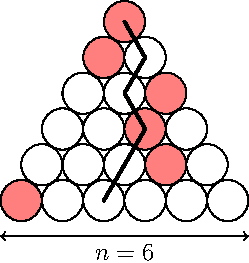
\includegraphics[scale=1]{Image/IMO2023.pdf}
        \end{center}
  Như một hàm số theo $n$, tìm lớn nhất $k$ sao cho trong mỗi tam giác Nhật Bản có một con đường ninja chứa ít nhất $k$ các vòng tròn màu đỏ.
    \end{btvn}
    \subsection{\LARGE \textcolor{dk}{Lời giải}}

    \newpage
    \thispagestyle{plain}
    
\includepdf[pages=1]{Image/bia/2.pdf}
    \section{\huge Phương trình hàm}
    \subsection{\LARGE \textcolor{dk}{Đề bài}}
    
    \item \begin{bt}\vocab{(USAMO 2002).}
        Tìm tất cả các hàm số $f: \mathbb{R} \to \mathbb{R}$ thỏa mãn
        \[
           f(x^2 - y^2) = xf(x) - yf(y)
        \]
        với mọi số thực $x,y$.
    \end{bt}
    \begin{sol}
        Ký hiệu $P(x,y)$ chỉ phép thế vào $(?)$ tương ứng. $P(x,0)$ ta được $f(x^2) = xf(x)$. Thay $x \to -x$ ta được $f$ là hàm lẻ. Viết Lại
        \[
            f(x^2 - y^2) = f(x^2) - f(y^2), \xyr
        \]
        Hay $f(x - y) = f(x) - f(y) ,\forall x, y \geq 0$. Thay $x \to x + y$ ta được $f(x) + f(y) = f(x + y), \forall x,y \geq 0$. Mặt khác lại có 
        \[
            -f(x) - f(y) = -f(x + y) \lra f(-x) + f(-y) = f(-x-y),\forall x,y \geq 0
        \]
        Suy ra $f$ cộng tính trên $\bb{R}$. Thế nên với mọi $k \in \bb{Q}$ ta có $f(kx) = kf(x)$. Đặt $a = f(1)$. Với $x \in \bb{R}$ và $y \in \bb{Q}$. Ta sẽ tính $f((x + y)^2)$ bằng hai cách. Ta có 
        \[
        f((x + y)^2) = (x + y)f(x + y) = (x + y)(f(x) + ay) = xf(x) + yf(x) + axy + ay^2
        \]
        Lại có 
        \[
        f((x + y)^2) = f(x^2 + 2xy + y^2) = f(x^2) + f(2xy) + f(y^2) = xf(x) + 2yf(x) + ay^2
        \]
        Cố định $x$ và so sánh hệ số của $y$ của hai cách, ta được $\boxed{f(x) = ax, \xr}$ và $a \in \bb{R}$.
    \end{sol}
    \item \begin{bt}\vocab{(IMO Shortlist 2017 A4).}
        Tìm tất cả các hàm số $f: \mathbb{R} \to \mathbb{R}$ thỏa mãn
        \[
           f(f(x)f(y)) + f(x + y) = f(xy)\tag{1}
        \]
        với mọi số thực $x,y$.
    \end{bt}
    \begin{sol}
        Ký hiệu $P(x,y)$ chỉ phép thế vào $(?)$ tương ứng. 
    
        Từ $(1)$ thay $P(0,0) \ra f(f(0)^2) = 0$. Đặt $c = f(0)^2$ thì $f(c) = 0$. 
    
        Giả sử $c \neq 1$. Khi đó thay $P\left(\frac{c}{c - 1},c\right) \ra f(0) = 0$.
    
        Từ $(1)$ thay $P(x,0) \ra f(x) = 0, \xr$. Thử lại thì thấy hàm này thỏa mãn. Giả sử tồn tại $x_0$ để $f(x_0) \neq 0$, khi đó đồng nghĩa với $c = 1$, hay $f(1) = 0$ và $f(0)^2 = 1$. Nói cách khác, nếu $f(c) = 0$ thì $c = 1$.
        
        \vocab{Trường hợp 1:} $f(0) = - 1$. 
        
        \vocab{Nhận xét 1:} $f(x + n) = f(x) + n, \xr, n \in \bb{N}$. 
        
        \begin{proof} Ta chứng minh điều này đúng bằng quy nạp. 
          Từ $(1)$ thay $P(x,1)$ ta được $f(x + 1) = f(x) + 1$. Giả sử với $n - 1 \in \bb{Z^+}$ ta có $f(x + n - 1) = f(x) + n - 1$, khi đó 
          \[
          f(x + n) = f(x + n - 1 + 1) = f(x + 1) + n - 1 = f(x) + n ,\xr
          \]
          Vậy nên $f(x + n) = f(x) + n, \xr, n \in \bb{N}$
        \end{proof}
        \vocab{Nhận xét 2: } Nếu $f(t) = - 1$ thì $t = 0$. 
        \begin{proof}
          Giả sử $t \neq 0$ mà $f(t) = -1$. Từ $(1)$ thay $P(t , 1)$ ta được
          \[
            f(0) + f(t + 1) = f(t)
            \lra f(t + 1) = 0
            \lra t + 1 = 1
            \lra t = 0
          \]
          Dẫn đến vô lý, vậy nên $t = 0$.
        \end{proof}
        \vocab{Nhận xét 3:} Nếu có $u,v \in \bb{R}$ mà $f(u) = f(v)$ thì \(
          \left\{
          \begin{array}{l}
          f(2u) = f(2v) \\
          f(-u) = f(-v) \\
          f(u^2) = f(v^2)
          \end{array}
          \right.
          \)
          \begin{proof}
            Giả sử có $f(a) = f(b)$. Lần lượt thay $P(x,a)$ và $P(x,b)$ vào $(1)$ ta được 
            \[
              f(x + a) - f(x + b) = f(xa) - f(xb) \tag{2}
            \]
            Thay $x \to 2$ vào $(2)$ thì được
            \[
              f(a + 2) - f(b + 2)  = f(2a) - f(2b) \lra f(2a) - f(2b) = f(a) + 2 - f(b) - 2 = 0
            \]
            Tương tự vậy thay $x \to -1 $ vào $(2)$ với chú ý $f(x - 1) = f(x) - 1,\xr$ ta được $f(-a) = f(-b)$.
    
            Từ $(1)$ thay lần lượt $P(a,a)$ và $P(b,b)$ ta được $f(a^2) = f(b^2)$.
          \end{proof}
          \vocab{Nhận xét 4: }$f$ là hàm đơn ánh trên $\bb{R}$.
          \begin{proof}
            Giả sử có $a,b \in \bb{R}$ mà $f(a) = f(b)$, đặt $d = a - b$. Ta sẽ chứng minh rằng $d = 0$. 
            
            Trong phép thế vào $(1)$:
    
            $P(a,-b) \ra f(f(a)f(-b)) + f(d) = f(-ab)$ 
    
            $P(-a,b) \ra f(f(-a)f(b)) + f(-d) = f(-ab)$ 
    
            Kết hợp lại ta được $f(d) = f(-d)$. 
            Mặt khác, với chú ý $d + b = a$ và $a - d = b$
    
            $P(d,b) \ra f(f(d)f(b)) + f(a) = f(db)$
    
            $P(-d,a) \ra f(f(-d)f(a)) + f(b) = f(-da)$
    
            Suy ra $f(db) = f(-da)$. Theo \vocab{nhận xét 3} thì ta được $f(da) = f(-db)$. Chú ý rằng $da - db = d^2$ và $ -da + db = -d^2$, tiếp tục thay
    
            $P(da,-db) \ra f(f(da)f(-db)) + f(d^2) = f(-d^2ab)$
    
            $P(-da,db) \ra f(f(-da)f(db)) + f(-d^2) = f(-d^2ab)$
            
            Kết hợp lại thì ta được $f(d^2) = f(-d^2)$. Lại có 
            
            $P(d,d) \ra f(f(d)^2) + f(2d) = f(d^2)$ 
    
            $P(d,-d) \ra f(f(d)f(-d)) + f(0) + f(-d^2)$
    
            Từ đây suy ra $f(2d) = f(0) = - 1$. Mà theo \vocab{nhận xét 2} thì được $2d = 0 \lra d = 0 \lra a = b$. Suy ra $f$ đơn ánh trên $\bb{R}$
          \end{proof}
    
          Khi này từ $(1)$ thay $P(x,1-x)$ ta được
          \[
          f(f(x)f(1-x)) + f(1) = f(x(1-x)) \lra f(f(x)f(1 - x)) = f(x(1-x)),\xr
          \]
          Vì $f$ đơn ánh nên \[f(x)f(1-x) = x(1-x),\xr \tag{3}\]
          Ta có 
          \[
            (3) \lra f(x)(f(-x) + 1) = x - x^2 \lra f(x) + f(x)f(-x) = x - x^2, \xr\tag{4}
          \]
          Thay $x \to -x$ ta được
          \[
            f(-x) + f(-x)f(x) = -x - x^2, \xr
          \]
          Suy ra $f(-x) = f(x) - 2x$. Thay biểu thức này vào $(4)$ ta được
          \[
            f(x) + f(x)(f(x) - 2x) = x - x^2 \lra f(x)^2 + (1 - 2x)f(x) +x^2 - x = 0
          \]
          Xét theo nghiệm là $f(x)$ ta có $\Delta  = (1 - 2x)^2 - 4(x^2 - x) = 4x^2 - 4x + 1 - 4x^2 + 4x = 1$. Giải phương trình này ta được $f(x) = x - 1,\xr$ hoặc $f(x) = x,\xr$.
          Thử lại thì hàm $f(x) = x$ không thỏa mãn.
          
          Giả sử tồn tại $a \in \bb{R}$ mà $f(a) = a$. 
          
          Từ $(1)$ thay $P(a,0) \ra f(-a) + a = -1 \lra f(-a) = -1 - a$ 

          Thay $P(-a,0) \ra f(a + 1) -a - 1 = -1 \lra a + 1 - a - 1 = -1$, vô lý.
          Vậy nên hàm thỏa mãn là $f(x) = x - 1, \xr$.

          \vocab{Trường hợp 2:} $f(0) = 1$. Để ý rằng khi thay hàm $f(x)$ bởi hàm $-f(x)$ vào $(1)$ hàm này vẫn thỏa mãn, tức là $-f(x)$ cũng là nghiệm của $(1)$, mà $-f(0) = -1$. Vậy nên giải tương tự với \vocab{trường hợp 1} thì ta được $f(x) = 1 - x, \xr$. 
    
          Vậy tất cả hàm số thỏa mãn là \[\boxed{f(x) = 0, \xr}, \boxed{f(x) = x - 1, \xr}, \boxed{f(x) = 1 - x, \xr}\]
      \end{sol}



    \item \begin{bt}\vocab{(IMO 2015).}
        Tìm tất cả các hàm số $f: \mathbb{R} \to \mathbb{R}$ thỏa mãn
        \[
           f(x + f(x + y)) + f(xy) = x + f(x + y) + yf(x)\tag{1}
        \]
        với mọi số thực $x,y$.
    \end{bt}
    \begin{sol}
        Ký hiệu $P(x,y)$ chỉ phép thế vào $(1)$. Gọi $\bb{S} = \{t \mid f(t) = t\}$ là tập hợp điểm bất động. 

        $P(x,1) \ra f(x + f(x + 1))  = x + f(x + 1), \xr \ra x + f(x + 1) \in \bb{S}$ 

        $P(0,0) \ra f(f(0)) = 0$. 

        $P(0,f(0)) \ra 2f(0) = f(0)^2$

        \vocab{Trường hợp 1:} $f(0) = 2$. 
       
        Xét $t$ là một điểm bất động bất kỳ của $\bb{S}$. 
        
        $P(t,0) \ra t + 2 = 2t \lra t = 2$. Mặt khác  $x + f(x + 1) \in \bb{S}$ thế nên $x + f(x + 1) = t = 2 \lra f(x) = 2 - x, \xr$
       
        \vocab{Trường hợp 2:} $f(0) = 0$.

        $P(0,x) \ra f(f(x)) = f(x) \ra f(x) \in \bb{S}$ 


        $P(-x,x) \ra f(-x) + f(-x^2) = -x +xf(-x) (2)$. 
        
        Cho $x  = 1$ ta được $2f(-1) = -1 +f(-1) \ra f(-1) = -1$

        $P(x,-x) \ra f(x) + f(-x^2) = x -xf(x) (3)$. 
        
        Cho $x = 1$ ta được $f(1) = 1$.
        

        $P(x- 1, 1) \ra f(x - 1 + f(x))  = x - 1 +f(x) \ra x - 1 + f(x) \in \bb{S}$

        $P(1, f(x) + x - 1) \ra f(x + 1 + f(x)) = x + 1  + f(x) \ra x + 1 + f(x) \in \bb{S}$.

        $P(x,-1)\ra f(x + f(x - 1)) + f(-x) = x + f(x - 1) - f(x) \lra f(-x) = -f(x), \xr$
        
        Từ $(2)$ và $(3)$ suy ra $f(-x) - f(x) = -2x +x(f(-x) + f(x)) \lra -2f(x) = 2x \lra f(x) = x, \xr$.

        Vậy các hàm số thỏa mãn là $\boxed{f(x) = 2-x,\xr}$ và $\boxed{f(x) = x,\xr}$
    \end{sol}
    \item \begin{bt}\vocab{(Vietnam TST 2022).}
         Cho số thực $\alpha$ và xét hàm số $\varphi(x)=x^2 e^{\alpha x}$ với mọi $x \in \mathbb{R}$. Tìm tất cả hàm số $f: \mathbb{R} \rightarrow \mathbb{R}$ thỏa mãn
            $$
            f(\varphi(x)+f(y))=y+\varphi(f(x))
            $$
            với mọi số thực $x, y$.
    \end{bt}
   
    \begin{sol}
        Ký hiệu $P(x,y)$ chỉ phép thế vào $(1)$. 

        $P(0,y) \ra f(f(y)) = y + \varphi(f(0)),\yr$. Từ đây dễ dàng suy ra $f$ song ánh. Khi đó $\exists c: f(c) = 0$.

        $P(c,f(y)) \ra f(\varphi(c) + f(f(y))) = f(y) $. Vì $f$ song ánh nên $\varphi(c) + f(f(y)) = y \lra \varphi(c) + y + \varphi(f(0)) = y \lra \varphi(c) + \varphi(0) = 0$.

        Mà vì $\varphi: \bb{R} \to [0,+\infty)$ nên $f(0) = c = 0$. 

        Từ $(1)$ thay $P(x,0) \ra f(\varphi(x)) = \varphi(f(x)) , \xr$. Suy ra $f(f(y)) = y$. Vì $\varphi(x)$ là hàm liên tục trên $\bb{R}$ và nhận mọi giá trị trong $[0,+\infty)$ nên $f(x) \geq 0, \forall x \geq 0$. $P(x,f(y))$ viết lại 
        \[
            f(\varphi(x) + y) = f(y) + f(\varphi(x)) \lra f(x + y) = f(x) + f(y), \forall x \geq 0, y \in \bb{R}
        \]
        Với $x,y\in \bb{R}$ chọn $z > \max\{0,-y\}$ ta có 
        \[
        f(x + y) + f(z) = f(x + y + z) = f(x) + f(y + z) = f(x) + f(y) + f(z)
        \]
        Suy ra $f$ cộng tính trên $\bb{R}$. Ta phát biểu và chứng minh bổ đề sau:
        \begin{lemma}
            Xét hàm số $f: \bb{R} \to \bb{R}$ bị chặn trên $[a,b]$ và thỏa mãn 
            \[
            f(x + y) = f(x) + f(y),\xyr
            \]
            Khi đó $f$ tuyến tính trên $\bb{R}$.    
        \end{lemma}
        \begin{proof}
            Giả sử tồn tại hàm $f: \mathbb{R} \rightarrow \mathbb{R}$ bị chặn trên đoạn $[a , b]$ và thỏa mãn điều kiện trên
            
            Do $f$ bị chặn trên đoạn $[a , b]$ nên $\exists M \in \mathbb{R}$ sao cho
            $$
            f(x)<M, \forall x \in[a , b] .
            $$

            Ta sẽ chứng minh hàm số $f$ cũng bị chặn trên đoạn $[0 , b-a]$.
            Thật vậy, với mọi $x \in[0 , b-a]$ thì $x+a \in[a , b]$. Ta có
            $$
            f(x+a)=f(x)+f(a) \Rightarrow f(x)=f(x+a)-f(a) \Rightarrow-2 M<f(x)<2 M .
            $$

            Vậy $|f(x)|<2 M, \forall x \in[0 , b-a]$, hay $f$ cũng bị chặn trên đoạn $[0 , b-a]$.
            Đặt $b-a=d>0$, khi đó $f$ bị chặn trên $[0 , d]$. Đặt $c=\frac{f(d)}{d}, g(x)=f(x)-c x$. Khi đó với mọi $x \in \mathbb{R}, y \in \mathbb{R}$ thì
            $$
            g(x+y)=f(x+y)-c(x+y)=f(x)-c x+f(y)-c y=g(x)+g(y) .
            $$

            Hơn nữa $g(d)=f(d)-c d=0$. Vậy $g(x+d)=g(x), \forall x \in \mathbb{R}$, hay $g$ là hàm tuần hoàn, hơn nữa $g$ cũng bị chặn trên $[0,d]$, kết hợp với tính tuần hoàn của $g$ trên $\bb{R}$, suy ra $g$ bị chặn trên $\bb{R}$. Giả sử tồn tại $x_0$ để $g(x_0) \neq 0$. Khi đó với $n \in \bb{N}$ thì $g(nx_0) = ng(x_0)$, suy ra 
            \[
                |g(nx_0)| = n|g(x_0)|, \forall n \in \bb{N}
            \]
            Do $g(x_0) \neq 0$ nên từ $(2)$ ta có $\dlim|g(nx_0)| =  \dlim|ng(x_0)| = +\infty$, do đó $|g(nx_0)|$ không bị chặn, mẫu thuẫn. Vậy $g(x) = 0, \xr$. Do đó $\boxed{f(x) = cx, \xr}$. Thử lại thì thỏa mãn.
        \end{proof}
        Áp dụng bổ đề trên ta được $f(x) = cx, \xr$, thử lại tìm được $c = 1$. Vậy hàm số thỏa mãn là $\boxed{f(x) = x, \xr}$
    \end{sol}

   
    \item \begin{bt}\vocab{(Romania EGMO TST 2022).}
        Tìm tất cả hàm số $f: \mathbb{R} \rightarrow \mathbb{R}$ thỏa mãn
            $$
            f(f(x)+y)=f\left(x^2-y\right)+4 y f(x)
            $$
            với mọi số thực $x, y$.
    \end{bt}
    \begin{sol}
        Ký hiệu $P(x,y)$ chỉ phép thế vào $(1)$. $P\left(x,\frac{x^2 - f(x)}{2}\right)$ ta được 
        \[
            (x^2 - f(x))f(x) = 0
        \]
        Khi đó có $f(0) = 0$. Dễ thấy rằng $f(x) = 0 ,\xr$ và $f(x) = x^2, \xr$ là hai hàm thỏa mãn. Giả sử tồn tại $a,b \neq 0$ thỏa mãn $f(a) = 0$ và $f(b) = b^2$. 

        Lại có $P(0,y)$ suy ra $f$ là hàm chẵn. Giả sử tồn tại $a,b > 0$ thỏa mãn $f(a) = 0$ và $f(b) = b^2$.

        $P(b,-a) \ra f(b^2 - a) = f(b^2 + a) -4ab^2$

        $P(a,y) \ra f(y) = f(a^2 - y) \ra f(y) = f(a^2 + y),\yr$ 

        $P(b,a^2) \ra f(b^2 + a^2) = f(b^2 - a^2) +4yb^2$ 
        
        $\lra f(a^2 + b^2) = f(a^2 - b^2) + 4a^2b^2 \lra f(b^2) = f(-b^2) + 4a^2b^2 \lra 4a^2b^2 = 0 $ 

        Vô lý vì $a, b \neq 0$. Vậy các hàm số thỏa mãn là $\boxed{f(x) = 0 ,\xr}, \boxed{f(x) = x^2 ,\xr}$.
    \end{sol}
    

    \item \begin{bt}\vocab{(IMO Shortlist 2004).}
        Tìm tất cả các hàm số $f: \mathbb{R} \to \mathbb{R}$ thỏa mãn
        \[
           f(x^2 + y^2 +2f(xy)) = \left(f(x + y)\right)^2
        \]
        với mọi số thực $x,y$.
    \end{bt}
    \begin{sol}
        Ký hiệu $P(x,y)$ chỉ phép thế vào $(?)$. Đặt $m = x^2 + y^2, n = xy$, khi đó $m^2 \geq 4n$, đặt $g(x) = 2f(x) - 2x$, viết lại 
        \[
            f(m^2 +g(n)) = f(m)^2, m^2 \geq 4n\tag{1}
        \]
        Gọi $c = f(0) = g(0)$, từ $(1)$ thay $P(m,0) \ra f(m^2 + c) =f(m)^2, \forall m \in \bb{R}, (2)$ 

        \vocab{Nhận xét 1: }$f(x) \geq 0,\forall x \geq c \geq 0 (3)$
        
        \begin{proof}
        Giả sử $c < 0$.
        
        Từ $(2)$ thay $m \to \sqrt{-c}$ ta được  $f(0) = f(\sqrt{-c})^2 \lra c = f(\sqrt{-c})^2 \geq 0$, vô lý.

        Suy ra $f(x + c) = f(\sqrt{x})^2 \geq 0, \forall x \geq 0$.
        \end{proof}
        

        \vocab{Nhận xét 2:} $f$ là hàm hằng khi $x > c$.
        \begin{proof}
            Nếu $g$ là hàm hằng thì dễ dàng thấy $f(x) = x, \xr$ là một nghiệm. Giả sử $g$ khác hằng. Xét $p_1 > p_2 \in \bb{R}$ bất kỳ sao cho $g(p_1) \neq g(p_2)$ và $u > v > \max\{4p_1,4p_2,c\}$ tùy ý sao cho $u^2 - v^2 = g(p_1) - g(p_2) = d$, với $d$ là hằng số. Khi đó có 
        \[
                g(p_1) + v^2 = g(p_2) + u^2
        \]
        Khi này ta được 
        \[
            f(v)^2 = f(v^2 + g(p_1)) = f(u^2 + g(p_2)) =f(u)^2 
        \]
        Vì $u,v > c$ nên $f(v), f(u) \geq 0$, thế nên $f(u) = f(v)$. Ta có 
        \[
        g(v) - g(u) = 2(f(v) - f(u) -v + u) = 2(u - v) = \frac{2d}{u + v} = t
        \]
        với $t$ tùy ý. Ta sẽ chứng minh rằng $g(u) - g(v)$ toàn ánh trên một đoạn nào đó. Thật vậy, bản chất của việc này là chứng minh hệ phương trình này theo $u,v$ có nghiệm
        \[
          \left\{
          \begin{array}{l}
          \frac{2d}{u + v} = t\\
          u^2 - v^2 = 2d
          \end{array}
          \right.
        \]
        Giải hệ ta dễ dàng tìm được \(
          \left\{
          \begin{array}{l}
          u = \frac{d}{t} + \frac{t}{2}\\
          v = \frac{d}{t} - \frac{t}{2}
          \end{array}
          \right.
        \)
         
        Ngược lại, với cách chọn $u,v$ như thế thì ta sẽ được $g(u) - g(v)$ nhận một giá trị $t > 0$ tùy ý. Chọn $u,v$ thuộc đoạn $[M,3M]$ với $M > \max\{4p_1,4p_2,c\}$. Khi đó $g(u) - g(v)$ sẽ toàn ánh trên $[\delta,2\delta]$ đủ nhỏ, tức là $f$ là hàm hằng trên $[\delta,2\delta]$. 

        Xét $p_1' = u$ và $p_2' = v$ và thực hiện tương tự thế, ta sẽ được nếu $a > b > L$ và $a^2 - b^2 \in [\delta,2\delta]$ thế thì $f(a) = f(b)$, với $L = 12M$ đủ lớn. Khi đó ta sẽ được $L^2 + \delta \leq a^2 ,b^2 \leq L^2 + 2\delta$, suy ra $f$ là hàm hằng trên $[\sqrt{L^2 +  \delta},\sqrt{L^2 + 2\delta}]$. Tương tự vậy, $f$ sẽ là hàm hằng trên đoạn $[\sqrt{L^2 +  2\delta},\sqrt{L^2 + 3\delta}]$, $[\sqrt{L^2 +  3\delta},\sqrt{L^2 + 4\delta}]$,\dots. Vậy nên hoàn tất chứng minh
        \end{proof}

        Xét $x,y$ thỏa mãn $y > x \geq 2\sqrt{M}$ và $\delta < y^2 -x^2 < 2\delta$. Khi đó tồn tại $u,v$ sao cho $x^2 + g(u) = y^2 + g(v)$. Ta được $f(x)^2 = f(y)^2$. Theo $(3)$ thì $f(x) = k$ với $x \geq 2\sqrt{M}$. Thay vào đề bài thì ta tìm được $k^2 = k$

        Từ đề bài cho $t = 0$ ta được $|f(z)| = |f(-z)| \leq 1, z \leq -2\sqrt{M}$. Ta có $g(u) = 2f(u) - 2u \geq - 2-2u$ với $u \leq -2\sqrt{M}$ cho $u \to -\infty$ thì có được $g$ không bị chặn trên. Khi đó với mỗi $z$ tồn tại $z'$ sao cho $z + g(z') > 2\sqrt{r}$. Thế thì $f(z)^2 = f(z^2 + g(z')) = k = k^2$. 
        
        Rõ ràng $f(z) = \pm k$ với mỗi $z$. Với $k = 0$ thì $f(x) = 0$ là một nghiệm của phương trình. Với $k = 1$ ta có $c = 2f(0) = 2$, thế thì $f(x) = 1$ với mọi $x \geq 2$. Nếu $f(i) = - 1$ với $i < 2$ nào đó thế thì $i - g(i) = 3i + 2> 4i$. Giả sử $i - g(i) \geq 0$ thì đặt $j = i -g(i) > 4i$. Thế thì $f(j)^2 = f(j^2 + g(i)) = f(i) = -1$ vô lý. 
        
        Vì vậy nên $i - g(i) < 0$ và $i < \frac{-2}{3}$. 
        
        Vậy tất cả hàm số thỏa mãn là $\boxed{f(x) = 0 ,\xr}, \boxed{f(x) = 0 ,\xr}$ và 
        \[\boxed{ f(x)=
        \left\{\begin{array}{rr}-1,&x\in \left(-\infty,-\frac{2}{3}\right)\\
            1,&x\not\in \left(-\infty,-\frac{2}{3}\right)
        \end{array}
        \right.
        }
        \]
    \end{sol}
    \item \begin{bt}\vocab{(IMO Shortlist 2015 A4).}
        Tìm tất cả các hàm số $f: \mathbb{Z}\to \mathbb{Z}$ thỏa mãn
        \[
           f(m - f(n))  = f(f( m)) - f(n) -1\tag{1}
        \]
        với mọi số nguyên $m,n$.
    \end{bt}
    \begin{sol}
        Ký hiệu $P(m,n)$ chỉ phép thế vào $(1)$. 

        $P(m,f(m)) \ra f(m - f(f(m))) = -1$. Suy ra tồn tại $a \in \bb{Z}$ để $f(a) = -1$. 

        $P(m,a) \ra f(m + 1) = f(f(m)),\forall m,n\in \bb{Z}$

        Viết lại có 
        \[
            f(m - f(n)) = f( m + 1) -f(n) - 1, \forall m,n \in \bb{Z}
        \]
        Đặt $k = f(n) + 1$. Thay $m \to m + f(n)$ ta được 
        \[
            f(m) =  f(m + k) -k \lra f(m + k) = f(m) +k
        \]
        Bằng quy nạp, ta chứng minh được $f(m + nk) = f(m) + nk, n \in \bb{Z^+}$

        Thay $m \to m - nk$ ta được $f(m - nk) = f(m) - nk, \forall n \in \bb{Z^+}$. Do đó 
        \[
            f(m + nk) = f(m) + nk, \forall m,n \in \bb{Z}
        \]
    \end{sol}
    \item \begin{bt}\vocab{(IMO 2012).}
        Tìm tất cả các hàm số $f: \mathbb{Z} \to \mathbb{Z}$ thỏa mãn
        \[
          f(a)^2 + f(b)^2 + f(c)^2 = 2f(a)f(b) + 2f(b)f(c) + 2f(c)f(a)
        \]
        với mọi số nguyên $a,b,c$ thỏa mãn $a + b + c = 0$.
    \end{bt}
    
    
    
        \item \begin{bt}\vocab{(Japan MO Final 2019).}
            Tìm tất cả các hàm số $f: \mathbb{R}^+\rightarrow \mathbb{R}^+$ thỏa mãn
            \[f\left(\frac{f(y)}{f(x)}+1\right)=f\left(x+\frac{y}{x}+1\right)-f(x)\]
        \end{bt}
    
    
    \item \begin{bt}\vocab{(VMO 2022).}
        Tìm tất cả hàm số $f: \mathbb{R}^{+} \rightarrow \mathbb{R}^{+}$thỏa mãn
        \[
        f\left(\frac{f(x)}{x}+y\right)=1+f(y) \tag{1}
        \]
        với mọi số thực dương $x, y$.
    \end{bt}
    
    \begin{sol}
        Ký hiệu $P(x,y)$ chỉ phép thế vào $(1)$.

        \vocab{Cách 1:}

        Gọi $\bb{T} =\left\{\frac{f(x)}{x}| x \in \bb{R^+}\right\}$. Giả sử $T$ nhận nhiều hơn một giá trị. Gọi $t_1, t_2 \in \bb{T}$ sao cho $t_1 > t_2$. Khi đó tồn tại $a_1,a_2 > 0$ sao cho $t_1 = \frac{f(a_1)}{a_1}, t_2 = \frac{f(a_2)}{a_2}$. Lần lượt $P(a_1,y)$, $P(a_2,y)$ và so sánh, ta được 
        \[
            f(y + t_1) = f(y + t_2), \yro
        \]
        Thay $y \to y - t_2$ và đặt $\delta = t_1 - t_2 > 0$, ta được $f(y) = f(y + \delta), \forall y > t_2$. Bằng quy nạp dễ dàng chứng minh được 
        \[f(y) = f(y + n\delta),\forall y > t_2, n \in \bb{Z^+} \tag{2}\]
        
        Mặt khác, $P(x, \frac{f(x)}{x} + y)$ ta được 
        \[
            f\left(2\frac{f(x)}{x}+y\right)=2+f(y), \xyro
        \]
        Cũng bằng quy nạp, ta chứng minh được 
        \[
            f\left(n\frac{f(x)}{x}+y\right)=n+f(y), \xyro \tag{3}
        \]
        Từ $(3)$ thay $P(1,x - nf(1))$ thì được 
        \[
            f(x) = n + f(x - nf(1)) > n ,\forall x > nf(1)
        \]
        Khi này chọn $n_0 > \left\lfloor \frac{f(1)n}{\delta}\right\rfloor$, từ $(3)$ cho $n = n_0$ ta được $f(x) = f(x + n_0\delta) > n, \forall x > t_2$. Khi này cho $n \to +\infty$ và cố định $x$ (vì $x$ không phụ thuộc vào $n$) thì $f(x) \to +\infty$ vô lý. 

        Suy ra $t_1 = t_2$ hay $\bb{T}$ chỉ nhận duy nhất một giá trị.

        Vậy $f(x) = cx, \xro$ và $c > 0$. Thử lại tìm được $c = 1$. 

        Vậy hàm duy nhất thỏa mãn là $\boxed{f(x) = x, \xro}$.

        \vocab{Cách 2:}
        Từ đề bài thay $P(x, \frac{f(x)}{x} + y)$ ta được 
        \[
            f\left(2\frac{f(x)}{x} + y\right) = 2 + f(y)
        \]
        Bằng quy nạp ta chứng minh được 
        \[
            f\left(n\frac{f(x)}{x} + y\right) = n + f(y),\xyro
        \]
        Giả sử tồn tại $a,b$ sao cho $\frac{f(a)}{a} \neq \frac{f(b)}{b}$ và không mất tính tổng quát, giả sử $\frac{f(a)}{a} > \frac{f(b)}{b}$. 
        
        Lần lượt cho $P(a,y)$ và $P(b,y)$ ta được \[f\left(\frac{f(a)}{a} + y\right) = f\left(\frac{f(b)}{b} + y\right),\tag{2}\]

        Đặt $k = \frac{f(a)}{a} - \frac{f(b)}{b}$. Ta được $f(x) = f(x + k), x > \frac{f(b)}{b}$. Mặt khác, từ giả thuyết có 
        \[
            f\left(n\frac{f(x)}{x} + y\right) = n + f(y), \xyro
        \]
        hay $f(x) > n$ với $x > n\frac{f(a)}{a}$. Cố định $x$ chọn $n = [f(x)] + 2 > f(x)$ và số nguyên dương $m$ sao cho $x + mk  > n\frac{f(a)}{a}$, như vậy $f(x + mk)  > n > f(x) = f(x + mk)$ vô lý. Do đó $\boxed{f(x) = cx, \xro}$.

        \vocab{Cách 3:} Trước hết ta phát biểu và chứng minh bổ đề sau:
        \begin{lemma}
            Cho các hàm số $f, g, h: \mathbb{R}^{+} \rightarrow \mathbb{R}^{+}$thỏa mãn
            $$
            f(g(x)+y)=h(x)+f(y)
            $$
            với mọi số thực duơng $x, y$. Khi đó hàm $\frac{g(x)}{h(x)}$ là hàm hằng.
        \end{lemma}
        \begin{proof}
            Ký hiệu $P(x, y)$ chỉ khẳng định $f(g(x)+y)=h(x)+f(y), \forall x, y>0$. Từ $P(x, y-g(x))$ ta suy ra
                $$
                f(y-g(x))=f(y)-h(x), \forall x>0, y>g(x) .
                $$

                Với $x, y>0$ và $p, q \in \mathbb{Z}^{+}$sao cho $p g(x)-q g(y)>0$, từ các đẳng thức trên ta dễ dàng chứng minh được
                $$
                f(z+p g(x)-q g(y))=f(z)+p h(x)-q h(y)
                $$
                với mọi $z>0$. Nếu $p h(x)-q h(y)<0$, khi đó ta thay $(p, q)$ bởi $(k p, k q)$ với $k$ nguyên dương đủ lớn thì
                $$
                f(z)+p h(x)-q h(y)<0,
                $$
                vố lý. Như vậy
                $$
                p g(x)>q g(y) \Longrightarrow p h(x) \geq q h(y) \quad \forall x, y>0,
                $$
                hay
                $
                \frac{g(x)}{g(y)}>\frac{q}{p} \Longrightarrow \frac{h(x)}{h(y)} \geq \frac{q}{p} \quad \forall x, y>0 .
                $

                Giả sử $\frac{g(x)}{g(y)}>\frac{h(x)}{h(y)}$, khi đó ta có thể chọn $p, q \in \mathbb{Z}^{+}$sao cho
                $ 
                \frac{g(x)}{g(y)}>\frac{q}{p}>\frac{h(x)}{h(y)}
                $
                điều này mâu thuẫn với chứng minh trên. Vậy
                $$
                \frac{h(x)}{h(y)} \geq \frac{g(x)}{g(y)} \Longrightarrow \frac{h(x)}{g(x)} \geq \frac{h(y)}{g(y)} \quad \forall x, y>0 .
                $$

                Thay đổi vai trò $x, y$ trong đánh giá trên ta thu được $\frac{h(x)}{g(x)}=\frac{h(y)}{g(y)}=c \quad \forall x, y>0$.
        \end{proof}
        Trở lại bài toán. Giả sử tồn tại hàm số thỏa mãn.
        Áp dụng bổ đề trên ta suy ra tồn tại số thực dương $c$ sao cho
        $$
        \frac{f(x)}{x}=c \Longrightarrow f(x)=c x \quad \forall x>0
        $$
        Từ đây tìm được $c = 1$. Vậy hàm duy nhất thỏa mãn là $\boxed{f(x) = x, \xro}$.
    \end{sol}

    \item \begin{bt}\vocab{(Balkan MO 2022).}
        Tìm tất cả hàm số $f: \mathbb{R}^{+} \rightarrow \mathbb{R}^{+}$thỏa mãn
        \[
        f\left(y f(x)^3+x\right)=x^3 f(y)+f(x)\tag{1}
        \]
        với mọi số thực dương $x, y$.
    \end{bt}
    \begin{sol}
        Ký hiệu $P(x,y)$ chỉ phép thế vào $(1)$.
        
        \vocab{Nhận xét 1:} $f$ là hàm tăng ngặt trên $\bb{R^+}$. 
        \begin{proof}
            Từ $(1)$ ta có 
        \[
            f(yf(x)^3) > f(x), \xyro \tag{2}
        \]
        Từ $(2)$, thay $P\left(x,\frac{y}{f(x)^3}\right)$ ta được $f(x + y) > f(x), \xyro$. Suy ra $f$ là hàm tăng ngặt, nên $f$ cũng đơn ánh trên $\bb{R^+}$.
        \end{proof}

        \vocab{Nhận xét 2:} $\blim_{x \to 0}f(x) = 0$. 
        \begin{proof}
            Vì $f$ tăng ngặt và $f(x) > 0$ nên phải tồn tại $L = \blim_{x \to 0}f(x)$, ta có $f(x) > L, \xro$. Ta có 
            \[
            f(yL^3) < f(yf(x)^3 + x) = x^3f(y) + f(x), \xyro
            \]
            Cho $x \to 0^+$ thì được $f(yL^3) \leq L, \yro$. Thế nên $yL^3 = 0$ hay $L = 0$.
            
        \end{proof}
        \vocab{Nhận xét 3:} $f$ là hàm liên tục trên $\bb{R^+}$. 
        \begin{proof}
            Ta có $f(yf(x)^3 + x) - f(x) = x^3f(y), \xyro$. Đặt $h = yf(x)^3$, cho $x =x_0 > 0$ bất kỳ, $y \to 0^+$ thì $h \to 0^+$, ta được 
            \[
                \blim_{h \to 0} f(x_0 + h) - f(x_0) =  f(x_0) - f(x_0) = 0
            \]
            Vậy nên $f$ liên tục trên $\bb{R}^+$.
        \end{proof}
        
        \vocab{Nhận xét 4:} $f$ song ánh trên $\bb{R^+}$
        \begin{proof}
            Thật vậy từ $(1)$ cho $x \to +\infty$ thì ta được $\blim_{x \to +\infty} f(x) = +\infty$. Mà $f$ liên tục và không bị chặn trên nên $f$ toàn ánh. Suy ra $f$ song ánh trên $\bb{R^+}$.
        \end{proof}
        \vocab{Nhận xét 5:} $f(1) = 1$. 
        \begin{proof}
            Giả sử $f(1)  < 1$ thì $P\left(1,\frac{1}{1-f(1)^3}\right)$ suy ra $f(1) = 0$, vô lý.

            Giả sử $f(1) > 1$, thì vì $f$ song ánh nên tồn tại $t < 1$ để $f(t) = 1$. 
            
            $P(t,y) \ra f(y + t) = t^3f(y) + 1 > f(y) \lra 1 > (1 - t^3)f(y)$ vô lý vì $f$ không bị chặn trên. Vì vậy $f(1) = 1$
        \end{proof}
        \vocab{Nhận xét 6: }$f(q) = q, \forall q \in \bb{Q^+} (4)$ 
        \begin{proof}
            Thay $P(1,y)$ ta được $f(y + 1) = f(y) + 1, \yro$. Bằng quy nạp ta chứng minh được $f(y + n) = f(y) + n, \yro$ và $n \in \bb{Z^+}$. Cho $y \to 0^+$ ta được $f(n) = n,\forall n \in \bb{Z^+}$.

            Với $m,n \in \bb{Z^+}$, thay $P\left(m,\frac{n}{m}\right)$ ta được 
            \[
                    f(nm^2 + m) = m^3 + f\left(\frac{m}{n}\right) + f(m) \lra f\left(\frac{m}{n}\right) = \frac{m}{n}, \forall m,n \in \bb{Z^+}
            \]
        \end{proof}
        Khi này, với mọi số thực $x > 0$, ta chọn dãy $(u_n)$ thỏa mãn $u_n = \frac{\lfloor nx \rfloor}{n}, \forall n \in \bb{Z^+}$. Khi này ta có 
        \[
            \frac{nx - 1}{n} <  \frac{\lfloor nx \rfloor}{n} < \frac{nx + 1}{n} 
        \]
        Vì $f$ liên tục trên $\bb{R^+}$ nên
        \[
           \dlim \frac{nx - 1}{n} <\dlim u_n < \dlim\frac{nx + 1}{n} \ra \dlim u_n = x
        \]
        Từ $(4)$ thay $x = u_n$ ta được 
        \[
            \dlim f(u_n) = f(\dlim u_n) = \dlim u_n = x 
        \]
        Vậy hàm số duy nhất thỏa mãn là $\boxed{f(x) =x ,\xro}$.
    \end{sol}
    \item \begin{bt}\vocab{(Switzerland TST 2022).}
         Tìm tất cả hàm số $f: \mathbb{R}^{+} \rightarrow \mathbb{R}^{+}$thỏa mãn
        $$
        x+f(y f(x)+1)=x f(x+y)+y f(y f(x))
        $$
        với mọi số thực dương $x, y$.
    \end{bt}
    \begin{sol}
        Ký hiệu $P(x,y)$ chỉ phép thế vào $(1)$.
    
    
        

        \vocab{Nhận xét 1:} $f$ không bị chặn trên.
        \begin{proof}
            Từ $P\left(x,\frac{y}{f(x)} - 1\right)$ suy ra \[f(y) = xf\left(x + \frac{y-1}{f(x)}\right) + \frac{y - 1}{f(x)}f(y - 1) - x,\xro, y > 1 \tag{2}
            \]
            Từ $(2)$ ta cho $y \to +\infty$ thì vế phải $\to +\infty$ nên $\blim_{y \to +\infty} f(y) = +\infty$.
        \end{proof}

        \vocab{Nhận xét 2:} $f$ đơn ánh trên $\bb{R^+}$
        \begin{proof}
            Giả sử có $f(a)=f(b)$ mà $a > b$. Đặt $d = a - b,q = \frac{b}{a}, r= \frac{d}{a}$, ta có $d,q,r > 0$ và $q < 1$.
        
            Thay lần lượt $P(a,x),P(b,x) \ra a - af(a + x) = b - bf(b + x)$. 

            Cho $x \to x -b$ và đặt $\delta = 4b$ là một số đủ lớn, ta được 
            \[
                f(x + d) = qf(x) + r, \forall x > \delta \tag{$\clubsuit$ }
            \]

            Ta phát biểu và chứng minh bổ đề sau:
            \begin{lemma}
                Xét hàm số $f: \bb{R^+} \to \bb{R^+}$ thỏa mãn 
                \[
                    f(x + d) = qf(x) + r, \forall x > M
                \]
                với $M$ là một số thực dương đủ lớn với $q < 1$ và $d,r > 0$. Khi đó $\blim_{x \to +\infty} f(x) = \frac{r}{1 - q}$.
            \end{lemma}
            \begin{proof}
            Thay $x \to x + d$ thì được \[f(x + 2d) = qf(x + d) + r = q(qf(x) + r) +r = q^2f(x) + qr + r, \forall x > \delta\]

            Ta sẽ chứng minh điều này đúng bằng quy nạp khi thay $2$ bởi $n$. Giả sử có \[f(x + nd) = q^nf(x) + r\dsum_{i = 0}^n q^i, \forall x > \delta\tag{3}\]

            Từ $(3)$ thay $x \to x + d$ ta được 
            \[
                f(x + (n + 1)d) = q^nf(x + d) + r\dsum_{i = 0}^n q^i = q^n(qf(x) +r) +  r\dsum_{i = 0}^n q^i = q^{n + 1}f(x) +  r\dsum_{i = 0}^{n + 1} q^i
            \]
            Vậy là giả thuyết quy nạp được chứng minh.

            Từ $(3)$ ta viết lại 
            \[
                f(x + nd) = q^nf(x) + r.\frac{1 - q^{n}}{1 - q}, \forall x > \delta \tag{4}
            \]
            Từ $(4)$ cho $n \to +\infty$ với chú ý $q < 1$ ta có 
            \[
                \lim_{x \to +\infty} f(x) = \dlim f(x + nd) = \frac{r}{1 - q}
            \]
            Hoàn tất chứng minh.
            \end{proof}
            Áp dụng bổ đề trên cho $(\clubsuit)$ thì ta được $\blim_{x \to +\infty} f(x) = \frac{r}{1 - q}$.

            Nhưng theo \vocab{nhận xét 2} thì $f$ không bị chặn trên và $\blim_{x \to +\infty}f(x) = +\infty$ nên dẫn tới vô lý.

            Suy ra $q = 1$ hay $d = 0 \ra a = b$. Thế nên $f$ đơn ánh trên $\bb{R^+}$.
        \end{proof}

        Từ $(1)$ thay $P\left(x,\frac{y}{f(x)}\right)$ suy ra \[x + f(y + 1) = xf\left(x + \frac{y}{f(x)}\right) + \frac{y}{f(x)}f(y) ,\xyro \]

        Cho $x = y = 1$ ta được $f(2) = f(1 + \frac{1}{f(1)})$. Vì $f$ đơn ánh nên $f(1) = 1$. 

        Từ $(1)$ thay $P(1,x) \ra f(x) = \frac{1}{x}, \xro$. Thử lại thì thỏa mãn. Vậy hàm duy nhất thỏa mãn là $\boxed{f(x) = \frac{1}{x}, \xro}$. 
       \end{sol}
    \item \begin{bt}\vocab{(Taiwan TST 2022, Round 2).}
        Tìm tất cả hàm số $f: \mathbb{R}^{+} \rightarrow \mathbb{R}^{+}$thỏa mãn
        $$
        f\left(x+y^2 f(y)\right)=f(1+y f(x)) f(x)
        $$
        với mọi số thực dương $x, y$.
   \end{bt}
   \item \begin{bt}\vocab{(Czech-Polish-Slovak Match 2022).}
    Tìm tất cả hàm số $f: \mathbb{R}^{+} \rightarrow \mathbb{R}^{+}$thỏa mãn
   $$
   f\left(f(x)+\frac{y+1}{f(y)}\right)=\frac{1}{f(y)}+x+1
   $$
   với mọi số thực dương $x, y$.
\end{bt}

    \item \begin{bt}\vocab{(Japan MO Final 2021).}
        Tìm tất cả các hàm số $f: \mathbb{Z}^+\rightarrow \mathbb{Z}^+$ thỏa mãn hai điều kiện sau
        \[
            n \mid m \text{ và }f(n) \mid f(m) - n
        \]
    \end{bt}
    
    \item \begin{btvn}\vocab{(Indonesia TST 2022). }
        Tìm tất cả hàm số $f: \mathbb{R} \rightarrow \mathbb{R}$ thỏa mãn
        $$
        f\left(x^2\right)-f\left(y^2\right) \leq(f(x)+y)(x-f(y))
        $$
        với mọi số thực $x, y$.
    \end{btvn}

    \item \begin{btvn}\vocab{(Japan MO Final 2022).}
        Tìm tất cả các hàm số $f: \mathbb{Z}^+\rightarrow \mathbb{Z}^+$ thỏa mãn
        \[f^{f(n)}(m)+mn=f(m)f(n)\]
    \end{btvn}
    \item \begin{btvn}\vocab{(Hà Tĩnh TST 2023).}
        Tìm tất cả các hàm số $f: \bb{R} \to \bb{R}$ thỏa mãn 
        \[
            f(xf(x + y)) = f(yf(x)) + x^2
        \]
        với mọi số thực $x,y$.
    \end{btvn}
    \item \begin{btvn}\vocab{(Japan MO Final 2024).}
        Tìm tất cả các hàm số $f: \mathbb{Z}^+\rightarrow \mathbb{Z}^+$ thỏa mãn
        \[\text{lcm}(m, f(m+f(n)))=\text{lcm}(f(m), f(m)+n), \forall m,n \in \mathbb{Z}^+\]
    \end{btvn}


    \item \begin{btvn}\vocab{(VMO 2016).} Tìm tất cả hàm số $f:\mathbb{R} \to \mathbb{R}$ thỏa mãn:
        \begin{enumerate}
            \item $f(1) = 2016$
            \item $f(x+y+f(y))=f(x)+ay\quad\forall x,y\in\mathbb{R}$
        \end{enumerate}      
    \end{btvn}
    \item \begin{btvn}\vocab{(VMO 2017).} Tìm tất cả các hàm số $f:\mathbb{R} \to \mathbb{R}$ thỏa mãn:
        $$f(xf(y)-f(x))=2f(x)+xy$$
    với mọi số thực $x,y$.
    \end{btvn}
    \item \begin{btvn}\vocab{(VMO 2021).} Tìm tất cả các hàm số $f:\mathbb{R} \to \mathbb{R}$ thỏa mãn:
        \[f(x)f(y)=f(xy-1)+yf(x)+xf(y)\]
    với mọi số thực $x,y$.
    \end{btvn}
    \item \begin{btvn}\vocab{(VMO 2023).} Tìm tất cả các cặp hàm số $f,g:\mathbb{R} \to \mathbb{R}$ thỏa mãn $f(0) = 2022$ và
        \[f (x+g(y)) =xf(y)+(2023-y)f(x)+g(x)\]
    với mọi số thực $x,y$.
    \end{btvn}

    \item \begin{btvn}\vocab{(KMF 2022).}
    Tìm tất cả các hàm số $f,g: \mathbb{R} \to \mathbb{R}$ thỏa mãn:
    $$f(x^2-g(y))=g(x)^2-y, \forall x,y \in \mathbb{R}$$
    \end{btvn}

    \item \begin{btvn}\vocab{(Iran MO 2023).}
        Tìm tất cả các hàm số $f: \mathbb{C} \to \mathbb{C}$ thỏa mãn:
        \[
            f(f(x) + yf(y)) = x + |y|^2, \forall x,y \in \mathbb{C}
        \]
        Chú ý ở đây nếu $y = a + bi$ thì $|y| = \sqrt{a^2 + b^2}$, $a,b \in R$.
    \end{btvn}
    \item \begin{btvn}\vocab{(Balkan MO 2024).}
        Tìm tất cả các hàm số $f : \mathbb{R}^+ \to \mathbb{R}^+$ và đa thức $P(x)$ với hệ số thực không âm thỏa mãn $P(0) = 0$ và \[f(f(x) + P(y)) = f(x - y) + 2y\] với mọi số thực dương $x > y > 0$.
    \end{btvn}
    \item \begin{btvn}\vocab{(Vietnam TST 2014).} Tìm tất cả các hàm số $f:\mathbb{Z}\to \mathbb{Z}$ thỏa mãn:
        \[ f(2m+f(m)+f(m)f(n))=nf(m)+m \]
    với mọi số nguyên $m,n$.
    \end{btvn}
    \item \begin{btvn}\vocab{(Vietnam TST 2024).}Cho đa thức monic $P(x) \in \mathbb{R}[x]$ khác hằng. Tìm tất cả các hàm số liên tục $f: \mathbb{R} \to \mathbb{R}$ thỏa mãn
        $$f(f(P(x))+y+2023f(y))=P(x)+2024f(y),$$
        với mọi số thực $x,y$.
    \end{btvn}

    \item \begin{btvn}\vocab{(IMO Shortlist 2011 A3).}
        Tìm tất cả các cặp hàm số $f,g: \mathbb{R} \to \mathbb{R}$ thỏa mãn
        \[g(f(x+y)) = f(x) + (2x + y)g(y)\]
        với mọi số thực $x,y$.
    \end{btvn}


    \item \begin{btvn}\vocab{(IMO Shortlist 2018 A1).}
        Tìm tất cả các hàm số $f: \mathbb{Q}^+ \to \mathbb{Q}^+$ thỏa mãn
        $$f(x^2f(y)^2)=f(x)^2f(y)$$
        với mọi số hữu tỉ dương $x,y$.
    \end{btvn}

    \item \begin{btvn}\vocab{(IMO Shortlist 2018 A5).}
        Tìm tất cả các hàm số $f : \mathbb{R}^+ \mapsto \mathbb{R}$ thỏa mãn
        $$\left(x+\frac{1}{x}\right)f(y)=f(xy)+f\left(\frac{y}{x}\right)$$
        với mọi số thực dương $x,y$.
    \end{btvn}
    \item \begin{btvn}\vocab{(IMO Shortlist 2019 A1).}
        Tìm tất cả các hàm số $f: \mathbb{Z} \to \mathbb{Z}$ thỏa mãn
        $$f(2a)+2f(b)=f(f(a+b)).$$
        với mọi số nguyên $a,b$.
    \end{btvn}

    \item \begin{btvn}\vocab{(IMO Shortlist 2020 A6).}
        Tìm tất cả các hàm số $f: \mathbb{Z} \to \mathbb{Z}$ thỏa mãn
        \[f^{a^{2} + b^{2}}(a+b) = af(a) +bf(b)\]
        với mọi số nguyên $a,b$.
    \end{btvn}

    \item \begin{btvn}\vocab{(IMO Shortlist 2020 A8).}
        Tìm tất cả các hàm số $f : \mathbb{R} \mapsto \mathbb{R}$ thỏa mãn
        $$f(x+f(xy))+y=f(x)f(y)+1$$
        với mọi số thực $x,y$.
    \end{btvn}

    \item \begin{btvn}\vocab{(Đồng Tháp TST 2023).}
        Tìm tất cả các hàm số $f: \mathbb{R} \to \mathbb{R}$ thỏa mãn
        \[
            f(x + y) + f(x - y) - 2f(x)f(y + 1) = xy
        \]
        với mọi số thực $x,y$.
    \end{btvn}
    \item \begin{btvn}\vocab{(Bình Phước TST 2023).}
        Tìm tất cả các hàm số $f: \mathbb{R} \to \mathbb{R}$ thỏa mãn
        \[
            f(xf(x) + f(y)) = f(x)^2 + y
        \]
        với mọi số thực $x,y$.
    \end{btvn}
    \item \begin{btvn}\vocab{(An Giang TST 2023).}
        Tìm tất cả các hàm số $f: \mathbb{R} \to \mathbb{R}$ thỏa mãn
        \[
            f(x^2 + f(y)) = y + f(x)^2
        \]
        với mọi số thực $x,y$.
    \end{btvn}
    \item \begin{btvn}\vocab{(Thanh Hóa TST 2023).}
        Tìm tất cả các hàm số $f: \mathbb{R} \to \mathbb{R}$ thỏa mãn
        \[
            f(f(y) + x^2 + 1) + 2x = y + f(x + 1)^2
        \]
        với mọi số thực $x,y$.
    \end{btvn}


    \item \begin{btvn}\vocab{(PTNK 2023).}
        Tìm tất cả các hàm số $f: \bb{R} \to \bb{R}$ thỏa mãn $f(x + 1) =f(x) + 1$ và
        \[
            f(x^{2024} + x^{2023} + \dots + x + 1) = (f(x))^{2024} + (f(x))^{2023} + \dots + f(x) + 1
        \]
    \end{btvn}
    \item \begin{btvn}\vocab{(APMO 2023).}
        Cho số thực dương $c > 0$. Tìm tất cả các hàm số $f: \bb{R}^+ \to \bb{R}^+$ thỏa mãn
        \[
            f((c + 1)x +f(y)) = f(x + 2y) +2cx
        \]
        với mọi số thực dương $x,y$.
    \end{btvn}
    \subsection{\LARGE \textcolor{dk}{Lời giải}}
    \newpage
    \thispagestyle{plain}
    
\includepdf[pages=1]{Image/bia/3.pdf}
    \section{\huge Dãy số}
    \subsection{\LARGE \textcolor{dk}{Đề bài}}
    \item \begin{bt}\vocab{(Đồng Nai TST 2023).}
        Cho dãy số $(a_n)$ thỏa mãn $a_1 = 1$ và $$a_{n + 1} = \sqrt{2n + a_n^2 + \frac{1}{a_n}}, n \geq 1$$.
        \begin{enumerate}[label=(\alph*)]
            \item Chứng minh rằng $a_n \leq n$, với mọi số nguyên dương $n$.
            \item Tìm $\dlim a_n$
        \end{enumerate}
    \end{bt}
    \begin{sol}
        (a) Thật vậy, bằng quy nạp ta dễ dàng chứng minh được $a_n \geq 1, \forall n \geq 1$. Khi này, giả sử $a_{n} \leq n$, ta có 
        \[
            a_{n + 1} = \sqrt{2n + a_n^2 + \frac{1}{a_n}} \leq \sqrt{2n + n^2 + 1 } = \sqrt{(n + 1)^2} = n + 1
        \]
        hoàn tất chứng minh.

        (b) Ta có 
        \(
        a_{n + 1} \geq \sqrt{2n + 1 + \frac{1}{n}} 
        \). Cho $n \to +\infty$ thì ta được $\dlim a_n = +\infty$.
    \end{sol}
    \item \begin{bt}\vocab{(Hà Tĩnh TST 2023).}
        Cho dãy số $(u_n)$ xác định bởi $u_1 = 1$ và $$u_{n + 1} = 1 + \frac{1}{u_n + 1}, n \geq 1$$
        \begin{enumerate}[label=(\alph*)]
            \item Chứng minh rằng dãy số $(u_n)$ có giới hạn hữu hạn và tìm giới hạn đó.
            \item Chứng minh rằng $\dsum_{i = 1}^n u_i^2 < 2n, n \geq 1$.
        \end{enumerate}
    \end{bt}
    \begin{sol}
        (a) Ta cần chứng minh $\sqrt{2} \leq u_n \leq \frac{3}{2}, \forall n \geq 2$ bằng quy nạp. Với $n = 2$ thì rõ ràng luôn đúng, giả sử với $n\geq 2$ ta có $\sqrt{2} < u_{n} \leq \frac{3}{2}$, khi đó 
        \[
            u_{n + 1} = 1 + \frac{1}{u_n + 1} \leq 1 + \frac{1}{\sqrt{2} + 1}  \leq \frac{3}{2}
        \]
        \[
            u_{n + 1} = 1 + \frac{1}{u_n + 1} \geq 1 + \frac{1}{\frac{3}{2} + 1} > \sqrt{2}
        \]
        Khi này có đánh giá 
        \[
        |u_{n + 1} - \sqrt{2}| = \left|\frac{u_{n} + 2}{u_n + 1} -\sqrt{2}\right| \leq \left|\frac{u_n + 2}{\sqrt{2} + 1} - \sqrt{2}\right| = \frac{\left|u_n - \sqrt{2}\right|}{\sqrt{2} + 1} =\dots = \frac{1}{(\sqrt{2} + 1)^n}|u_1 -\sqrt{2}|
        \]
        Khi này tồn tại $N_0$ đủ lớn để $\forall n > N_0$ thì $\frac{1}{(\sqrt{2} + 1)^n}|u_n -\sqrt{2}| < \varepsilon \ra |u_{n + 1} - \sqrt{2}| < \varepsilon, \forall n > N_0$, suy ra $\dlim u_n = \sqrt{2}$.

        (b) Với chú ý $u_{n} > \sqrt{2},\forall n\geq 1$, ta có 
        \[
        \begin{aligned}
            \sum_{i = 1}^n u_i^2 = 1 + \sum_{i = 1}^{n - 1} \left(1 + \frac{1}{u_i+ 1}\right)^2 &= 1 + \sum_{i = 2}^{n - 1}1 + \frac{2}{u_i + 1} + \frac{1}{(u_i + 1)^2}\\
            &< 1  + \left(n -1 \right)\left(\frac{2}{\sqrt{2} + 1} + \frac{1}{(\sqrt{2} + 1)^2}\right)\\
            &=1 + (n - 1) = n
        \end{aligned}
        \]
        Chứng minh hoàn tất.
    \end{sol}
    \item \begin{bt}\vocab{(Hà Nội TST 2022).}
        Cho dãy $(x_n)$ được xác định bởi $x_1 = x_2 = 1$ và $x_{n + 2} = x_{n + 1}^2 - \frac{1}{3}x_n$ với $n \geq 1$. Chứng minh rằng $(x_n)$ có giới hạn hữu hạn và tìm giới hạn đó.
    \end{bt}
    \begin{sol}
        Ta có thể dự đoán rằng $\dlim x_n = 0$. Ta sẽ chứng minh $|x_n| < \frac{1}{3}$ bằng quy nạp. Với $n =4,5$ thì rõ ràng thỏa mãn, giả sử với $|x_{k}| < \frac{1}{3}, \forall 5 <k < n$.
        
        Khi đó ta có $|x_{n + 2}| < |x_{n + 1}^2| + \frac{1}{3}|x_n| < \frac{1}{3^2} + \frac{1}{3}.\frac{1}{3} < \frac{1}{3}$. Vậy nên từ đây ta được 
        \[
         |x_{n + 2}| < \frac{1}{3}|x_{n + 1}| + \frac{1}{3}|x_n|
        \]
        Theo bổ đề dãy số ta được $\dlim x_n = 0$.
    \end{sol}
    \item \begin{bt}\vocab{(PTNK 2023).}
        Cho dãy $(u_n)$ thỏa mãn $u_1 = 1$ và $u_{n + 1} = u_n + \frac{\ln n}{u_n}, n \geq 1$.
        \begin{enumerate}[label=(\alph*)]
            \item Chứng minh rằng $u_{2023} > \sqrt{2023 \ln 2023}$
            \item Tìm $\dlim\frac{u_n  \ln n}{n}$.
        \end{enumerate}
    \end{bt}
    \begin{sol}
        (a) Ta sẽ chứng minh $u_n >\sqrt{n\ln n}, \forall n > 4$ bằng quy nạp. Với $n = 5$ thì dễ dàng kiểm tra đúng, giả sử với $n - 1 > 4$ ta có $u_{n - 1} > \sqrt{n\ln n}$, khi đó 
        \[
            u_{n + 1} = \left(\frac{u_n}{n} + \frac{\ln n}{u_n}\right) + \frac{u_n(n - 1)}{n} > 2\sqrt{\frac{\ln n}{n}} +  \frac{n - 1}{n} \sqrt{n\ln n} = (n + 1)\sqrt{\frac{\ln n}{n}}
        \]
        Ta cần chứng minh $f(x) = \frac{\ln x}{x}$ là hàm giảm trên $(4,+\infty)$, thật vậy có $$f'(x) = \frac{1 - \ln x}{x^2} < 0, \forall x > 4$$ suy ra $\sqrt{\frac{\ln n}{n}} < \sqrt{\frac{\ln(n + 1)}{n + 1}}$, chứng minh hoàn tất, suy ra $u_{2023} > \sqrt{2023\ln2023}$

        (b) Đặt $L_n = \frac{u_n \ln n }{n}$, khi đó áp dụng định lý Stolz ta có $$\dlim L_n = u_{n + 1}\ln(n + 1) - u_n\ln n$$
        
        Mặt khác có $$u_{n + 1} - u_n = \frac{\ln n}{u_n} < \sqrt{\frac{\ln n }{n}}$$ Cho $n \to +\infty$ thì theo định lý kẹp, ta được \(\dlim (u_{n + 1} - u_n) = 0\). Khi này ta được 
        \[
        \begin{aligned}
            \dlim L_n &= \dlim\ln (n + 1)(u_{n + 1} - u_n) +u_n(\ln(n + 1) - \ln n)\\
            &= \dlim \frac{\ln(n + 1) \ln n}{u_n} + u_n \ln \left(\frac{n + 1}{n}\right)\\
            &\leq \dlim \sqrt{\frac{\ln(n + 1)^2\ln n}{n}} +\frac{u_n}{n}\frac{\ln\left(1 + \frac{1}{n}\right)}{\frac{1}{n}}\\
            &= 0 + 0 = 0
        \end{aligned}
        \]
        Vậy nên $\dlim \frac{u_n \ln n}{n} = 0$.
    \end{sol}
    \item \begin{bt}\vocab{(Trại hè Hùng Vương 2023).}
        Cho dãy số $(u_n)$ được xác định bởi $u_1 = 3$ và $$u_{n + 1} = u_n^2 + u_n - 4, n \geq 1$$ Tìm $\dlim\frac{(u_1 + 1)(u_2 + 3)\dots(u_n + 3)}{u_{n + 1} +3}$.
    \end{bt}
    \begin{sol}
        Bằng quy nạp, ta dễ dàng chứng minh được $u_n > 2, \forall n \geq 1$. Ta có 
        \[
            u_{n + 1} - 2 = (u_n - 2)(u_n + 3) \lra u_n + 3 = \frac{u_{n + 1} - 2}{u_n - 2}
        \]
        Cho nên từ đây viết lại $\dprod_{i = 1}^n (u_i + 3) = \dprod_{i = 1}^n \frac{u_{i + 1} - 2}{u_i - 2} = \frac{u_{n + 1} - 2}{3- 2} = u_{n + 1} - 2$. Mặt khác, bằng Weierstrass ta dễ dàng chứng minh được $\dlim u_n = +\infty$, nên từ đó tính được \[\dlim\frac{(u_1 + 1)(u_2 + 3)\dots(u_n + 3)}{u_{n + 1} +3} = \dlim \frac{u_n - 2}{u_n + 3} = 1\]
    \end{sol}
    \newpage
    
    \item \begin{bt}\vocab{(Bình Phước TST 2023).}
        Cho đãy số $\left(a_n\right)$ xác định bởi: \[\left\{\begin{array}{l}a_1=\frac{2024}{2023} \\ a_{n+1}=a_n+2 \sqrt{a_n}+\frac{n^2}{a_n}, \forall n \geq 1 .\end{array}\right.\]
        \begin{enumerate}[label=(\alph*)]
            \item Chứng minh rằng dãy số $\left(b_n\right)$ xác định bởi $b_n=\dsum_{i=1}^n \frac{1}{a_i}$ có giới hạn hữu hạn.
            \item Xét dãy số $\left(c_n\right)$ xác định bởi $c_n=\left[\dsum_{i=1}^n \frac{i}{a_i}\right]$.Chứng minh rằng mỗi số nguyên dương đều xuất hiện trong dãy $\left(c_n\right)$.
        \end{enumerate}
        
    \end{bt}
    \begin{sol}\textit{(Phạm Bảo)}

        (a) Vì đề bài chỉ yêu cầu chứng minh hội tụ mà không cần tính ra mà lại cho một cấu trúc dãy khá cồng kềnh, nên ta có thể nghĩ đến việc sử dụng các tiêu chuẩn hội tụ, ta xét tiêu chuẩn sau, xem như bổ đề: 
        \begin{theo}[Tiêu chuẩn D'Alembert]
            -Cho chuỗi số dương $\displaystyle \sum_{i = 1}^{\infty} a_i$ và tồn tại
            \(D = \dlim\frac{a_{n + 1}}{a_n}\)
            \begin{enumerate}
                \item Nếu $D > 1$ thì chuỗi phân kì.
                \item Nếu $D < 1$ thì chuỗi hội tụ.
                \item Nếu $D = 1$ thì chưa biết được chuỗi hội tụ hay phân kì.
            \end{enumerate}
        \end{theo}
        \begin{proof}

            1) Cho $D < 1$, khi đó chọn $\varepsilon > 0$ đủ nhỏ sao cho $\varepsilon > 1 - D$ theo định nghĩa giới hạn 
            \[
                \exists n_0: \forall n \geq n_0 \text{ sao cho }\frac{a_{n - 1}}{a_n} < D + \varepsilon
            \]
            Đặt $D + \varepsilon = q$, $0 < q < 1$ ta được $a_{n + 1} < qa_n$. Khi này chuỗi có thể viết lại thành 
            \[
            \dsum_{i = 1}^{+\infty}a_i < \dsum_{i = 1}^{+\infty}q^i a_1
            \]
            Vì $q < 1$ nên theo định nghĩa tổng vô hạn cấp số nhân thì chuỗi hội tụ.

            2) Cho $D > 1$, với $\varepsilon = D -1$, theo định nghĩa giới hạn 
            \[
                \exists n_0: \forall n \geq n_0 \text{ sao cho }\frac{a_{n - 1}}{a_n} > D - \varepsilon + 1 \ra a_{n + 1} > a_n
            \]
            Như vậy $a$ không thể tiến tới $0$ khi $n \to +\infty$. Vậy chuỗi phân kì 

            3) Ta có thể đưa ra một vài ví dụ và phản ví dụ để chứng minh trường hợp này.
        \end{proof}
        Quay trở lại bài toán, Dễ thấy $a_n > 0, \forall n \geq 1$. Chia hai vế cho $a_n$ ta được $\frac{a_{n + 1}}{a_n} = 1 + \frac{2}{\sqrt{a_n}} + \frac{n^2}{a_n^2}$, mặt khác lại có 
        \[
            \dlim D_n = \dlim \frac{\frac{1}{a_{n + 1}}}{\frac{1}{a_n}} = \dlim \frac{a_n}{a_{n + 1}} = \dlim \frac{1}{1 + \frac{2}{\sqrt{a_n}} + \frac{n^2}{a_n^2}} < 1
        \]
        Suy ra $\dlim D_n < 1$. Theo tiêu chuẩn D'Alembert thì $(b_n)$ hội tụ.

        (b) 
        Ta có một bổ đề sau 
        \begin{theo}[Bổ đề quan trọng]
            -Cho một dãy số thực $(a_n)$ thỏa mãn $0 < a_n \leq 1, \forall n \geq 1$ và $\dlim \dsum_{i = 1}^n a_n = +\infty$. Khi đó với mọi số nguyên dương $M$, luôn tồn tại $N > 0$ để với $n_0 > N$ nào đó thì 
            \[
            \left\lfloor \dsum_{i = 1}^{n_0} a_i \right\rfloor = M
            \]
        \end{theo}
        \begin{proof} Ta sẽ chứng minh bổ đề này bằng phản chứng. Đặt $b_n = \dsum_{i = 1}^n a_n$. Giả sử không tồn tại $N_0$ để thỏa mãn bổ đề, khi đó sẽ có hai trường hợp xảy ra. 

        \vocab{Trường hợp 1:} Không tồn tại $n_0$ để $\lfloor b_{n_0}\rfloor =M$ mà lại tồn tại $m_0$ để $\lfloor b_{m_0} \rfloor > M$. Để $(\lfloor b_n \rfloor)$ không nhận giá trị của $M$ mà lại nhận những giá trị nguyên lớn hơn nó thì phải tồn tại $a_k$ để $a_k > 1$, điều này là vô lý.

        \vocab{Trường hợp 2: } Không tồn tại $n_0$ để $\lfloor b_{n_0}\rfloor =M$ và cũng không tồn tại $m_0$ để $\lfloor b_{m_0} \rfloor > M$. Khi này rõ ràng là đến một lúc nào đó, sẽ tồn tại $m > 0$ và $N > 0$ để $b_{n_0} < m, \forall n_0 > N$, tức là $(b_n)$ bị chặn trên. Mặt khác $(b_n)$ cũng là dãy tăng, nên theo Weierstrass thì $(b_n)$ có giới hạn hữu hạn, cũng vô lý. 

        Vậy là bổ đề đã được chứng minh.
        \end{proof}
        Quay trở lại bài toán, đặt $s_n = \dsum_{i = 1}^n \frac{i}{a_i}$, ta có hai nhận xét:
        
        \vocab{Nhận xét 1:} $a_n \geq n,\forall n \geq 1$., sử dụng bất đẳng thức AM-GM, ta được 
        \[
            a_{n + 1} = (a_n + \frac{n^2}{a_n}) + 2\sqrt{a_n} \geq 2n + 2\sqrt{a_n} \geq n + 1 \ra a_n \geq n,\forall n \geq 1
        \]

        \vocab{Nhận xét 2: }$a_n \leq n^2, \forall n \geq 1$. Ta chứng minh điều này đúng bằng quy nạp. Với $n = 1$ thì dễ dàng kiểm tra, giả sử với $n > 1$ nào đó ta có $a_n \leq n^2$, ta xét hàm số $f(x) = x + 2\sqrt{x} + \frac{n^2}{x}$ trên đoạn $[n, +\infty)$. Ta có $f'(x) = 1 + \frac{1}{\sqrt{x}} - \frac{n^2}{x^2} \geq 1 + \frac{1}{x} - 1 \geq 0$, suy ra $f(x)$ là hàm tăng, vậy nên ta được 
        \[
        a_{n + 1} = a_n + 2\sqrt{a_n} + \frac{n^2}{a_n} \leq n^2 +2n + 1 = (n + 1)^2
        \]
        Hoàn tất quy nạp. Mặt khác, từ $(s_n)$ ta có $\frac{n}{a_n} \leq 1, \forall n \geq 1$ và \[s_n = \dsum_{i = 1}^n \frac{i}{a_i} > \dsum_{i = 1}^n \frac{i}{i^2} = \dsum_{i = 1}^n \frac{1}{i}\] Cho $n \to +\infty$ thì ta được $\dlim s_n = +\infty$. Khi đó, áp dụng bổ đề trên, ta có được điều phải chứng minh.
    \end{sol}
    \item \begin{bt}\vocab{(PTNK 2022).}
        Cho dãy số $(u_n)$ được xác định bởi $u_1 = 1$ và $u_{n + 1} = \sqrt{2 + u_n}, n \geq 1$. Tính
        \[
            \lim_{n \to + \infty} \frac{1}{\ln n}\left(\frac{u_1}{1} + \frac{u_2}{2} + \dots + \frac{u_n}{n}\right)
        \]
    \end{bt}
    \begin{sol}
        Đặt $u_1 = 2\cos\frac{\pi}{3}$, có $u_2 = \sqrt{2 + 2\cos\frac{\pi}{3} }= 2\cos\frac{\pi}{3.2}$. Bằng quy nạp, ta chứng minh được $u_n = \cos\frac{\pi}{3.2^{n - 1}}$. Theo định lý Stolz, ta có 
        \[
            \lim_{n \to + \infty} \frac{\frac{u_1}{1} + \frac{u_2}{2} + \dots + \frac{u_n}{n}}{\ln n } = \dlim \frac{\frac{u_{n + 1}}{n + 1}}{\ln(n + 1) - \ln(n)}= \dlim \frac{2\cos\frac{\pi}{3.2^{n}}}{\ln\left(1 + \frac{1}{n}\right)^n + \ln\left(1 + \frac{1}{n}\right)} = 2
        \]
        Vậy nên $\dlim \frac{1}{\ln n}\left(\frac{u_1}{1} + \frac{u_2}{2} + \dots + \frac{u_n}{n}\right) = 2$.
    \end{sol}

    \item \begin{btvn}\vocab{(Kon Tum TST 2023).} Cho các ý sau:
        \begin{enumerate}
            \item Cho dãy số $(u_n)$ được xác định bởi
            \[\left\{
                \begin{array}{l}
                    u_1 = 2 \\
                    u_n = u_{n - 1} + 2n + 3, \forall n \geq 1 
                \end{array}\right.\]
            Chứng minh rằng $u_n + 7$ là số chính phương với mọi $n \geq 1$.
            
            \item Cho dãy số $(u_n)$ được xác định bởi
            \[\left\{
                \begin{array}{l}
                    u_1 = 2023\\
                    u_{n + 1} = \frac{u_n^2 + 8}{2(u_n - 1)}, \forall n \geq 1
                \end{array}
            \right.
            \]
            Chứng minh dãy $(u_n)$ có giới hạn hữu hạn và tìm giới hạn đó.
        \end{enumerate}
    \end{btvn}
    \item \begin{btvn}\vocab{(Sóc Trăng TST 2023).} Với số thực $a$, xét dãy số $(u_n)$ xác định bởi
    \[
        u_1 = a \text{ và } u_{n + 1} = \frac{u_n^2}{2 - u_n^2}, n \geq 1
    \]
    \begin{enumerate}
        \item Chứng minh rằng với mọi $a$ hữu tỷ, các số hạng của $(u_n)$ luôn xác định.
        \item Với $a \in [0,1]$, chứng minh rằng dãy số $(v_n)$ xác định bởi $v_n = n^2 u_n$ luôn có giới hạn hữu hạn và xác định giới hạn đó.
    \end{enumerate}
    \end{btvn}
    \begin{btvn}\vocab{(Thanh Hóa TST 2023).} Cho dãy số $(u_n)$ được xác định bởi
        \[
            u_1 = \frac{1}{2} \text{ và } x_{n + 1} = \frac{1}{4} \left(x_n + \frac{3}{x_n}\right), n \geq 1
        \]
    Chứng minh rằng dãy số $(x_n)$ có giới hạn hữu hạn và tính giới hạn đó.
    \end{btvn}
    \item \begin{btvn}\vocab{(Tiền Giang TST 2023).}
        Cho dãy số $(a_n)$ được xác định bởi
        \[
            0 < a_1 \neq 1 \text{ và } a_{n + 1} = a_n + \frac{n}{a_n}, n \geq 1 
        \]
        \begin{enumerate}[label=(\alph*)]
            \item Chứng minh rằng $a_n > n, \forall n \geq 2$
            \item Tính $\lim (a_n - n)$
        \end{enumerate}
    \end{btvn}
    \item \begin{btvn}\vocab{\href{https://youtu.be/jsNmOM8S2po?si=H-oE95ze7Y6XjSO7}{(TST Phú Yên 2023).}}
        Cho hai dãy số $(u_n)$ và $(v_n)$ được xác định bởi
        \[
            \left\{
                \begin{array}{l}
                    u_1 = 4, v_1 = 2\\
                    u_{n + 1} = u_n^2 + 3v_n\\
                    v_{n + 1} =2u_nv_n
                \end{array}
            \right.
        \]
        Tìm $\displaystyle \lim_{n \to +\infty}\sqrt[2^n]{v_n}$ và $\displaystyle \lim_{n \to +\infty}\sqrt[2^n]{u_1u_2\dots u_n}$.
    \end{btvn}
    \item \begin{btvn}\vocab{\href{https://youtu.be/gqwfWR4fmEQ?si=M_6OgMGvI4iS9jHL}{(TST Quảng Bình 2023).}}
        Cho hai dãy số $(u_n)$ và $(v_n)$ được xác định bởi
        \[
            \left\{
                \begin{array}{l}
                    u_1 = 2024\\
                    (n + 1)^2u_{n + 1} =(n^2 + 2n)u_n + 2023, n \geq 1
                \end{array}
            \right.
        \]
        Tìm giới hạn của dãy số $(u_n)$.
    \end{btvn}
    \item \begin{btvn}\vocab{\href{https://youtu.be/3gCwGsteyO0?si=R2vB3_TBLXd6PYSw}{(Epsilon).}}
        Cho dãy số $\left(x_n\right)_{n=1}^{+\infty}$ như sau: $x_1=a>2$ và
            $$
            x_{n+1}=x_n^2-2, \forall n=1,2, \ldots
            $$
            Tính $\displaystyle\lim _{n \rightarrow+\infty}\left(\frac{1}{x_1}+\frac{1}{x_1 x_2}+\frac{1}{x_1 x_2 x_3}+\cdots+\frac{1}{x_1 x_2 \ldots x_n}\right)$.
    \end{btvn}
    \item \begin{btvn}\vocab{\href{https://youtu.be/3gCwGsteyO0?si=R2vB3_TBLXd6PYSw}{(Hà Tĩnh 2014).}}
        Cho dãy số $\left(u_n\right)$ thỏa mãn:
        $$
        \left\{\begin{array}{l}
        u_1=1 ; u_2=3 \\
        \frac{u_{n+1}}{u_n}=\frac{u_n^2}{u_{n-1}^2}-2, n \geq 1 .
        \end{array}\right.
        $$

        Chứng minh $\frac{1}{u_1}+\frac{1}{u_2}+\ldots+\frac{1}{u_n}<\frac{5-\sqrt{5}}{2}$ với mọi $n \geq 1$.
    \end{btvn}
    \item \begin{btvn}\vocab{(Gặp gỡ toán học 2010).}
        Cho dãy số $(x_n)$ được xác định bởi
        \[
            x_1 = 1, x_{n + 1} = x_n + \frac{1}{x_n}, \forall n \geq 1
        \]
        \begin{enumerate}
            \item Chứng minh rằng $\dlim x_n = +\infty$
            \item Tìm $\lim_{n \to +\infty}\frac{x_n}{\sqrt{n}}$.
        \end{enumerate}
    \end{btvn}
    \item \begin{btvn}\vocab{\href{https://youtu.be/PITrGXRwWgk?si=48dpyJynXmDHQDFs}{(Đồng Nai 2022).}}
        Cho dãy số dương $(u_n)$ được xác định bởi \[u_0 = 2, u_1 = 4 \text{ và } u_{n + 2} =2\sqrt{4u_{n + 1}^2 - u_nu_{n + 2}} + u_n\text{ với } n \geq 1\]
        \begin{enumerate}[label=(\alph*)]
            \item Tìm công thức tổng quát của $(u_n)$.
            \item Với mỗi số nguyên dương $n$. Đặt $S_n = \dsum_{i = 0}^n \frac{1}{u_i}$. Chứng minh rằng $(S_n)$ có giới hạn hữu hạn và tìm giới hạn đó.
        \end{enumerate}
    \end{btvn}
    \item \begin{btvn}\vocab{\href{https://youtu.be/gm3A3g_USIM?si=kokHTJ8RcjuvD2QJ}{(Epsilon).}}
        Cho dãy $(u_n)$ được xác định bởi 
        \[
            u_1 = 1, u_2 = 2, ( n + 1)u_{n + 2} = n(u_{n + 1} + u_n) + 2\left(u_{n + 1} + \frac{u_n}{n}\right) + 3u_n, \text{ với } n\geq 1 
        \]
        Chứng minh rằng dãy $\left(\frac{u_{n + 1}}{u_n}\right)_{n \geq 1}$ có giới hạn hữu hạn và tìm giới hạn đó.
    \end{btvn}
    \item \begin{btvn}\vocab{\href{https://youtu.be/ZkFer1ma5Ew?si=lX8buOq2Q-JVIyZG}{(Epsilon).}}
        Cho dãy số $(x_n)$ được xác định bởi $x_1 = 1$ và 
        \[
            x_{n + 1} = \frac{x_1}{n + 1} + \frac{x_2}{n + 2} +\dots+ \frac{x_n}{2n}, n \geq 1
        \]
        Chứng minh rằng $(x_n)$ có giới hạn hữu hạn và tìm giới hạn đó.
    \end{btvn}
    \item \begin{btvn}\vocab{(Korean MO 2022).}
    Cho ba dãy số $\{a_n\},\{b_n\},\{c_n\}$ thỏa mãn
    \[a_1=2,\,b_1=4,\,c_1=5\]
    \[\forall n,\; a_{n+1}=b_n+\frac{1}{c_n}, \, b_{n+1}=c_n+\frac{1}{a_n}, \, c_{n+1}=a_n+\frac{1}{b_n}\]
    Chứng minh rằng với mọi $n$ nguyên dương, $\max(a_n,b_n,c_n)>\sqrt{2n+13}$.
    \end{btvn}
    \item \begin{btvn}\vocab{\href{https://youtu.be/pAaUJ7SOZv8?si=7vxliQZNwqlyoAw-}{(Vũng Tàu 2022).}}
        Cho dãy số $(u_n)$ được xác định bởi $u_1 = 1$ và $u_{n + 1} = u_n + \frac{2}{u_n} + \frac{n}{u_n^4}$ với mọi $n$ nguyên dương. Tìm $\lim \frac{u_n}{\sqrt{n}}$.
        
    \end{btvn}
    \item \begin{btvn}\vocab{(Korean MO 2022).}
        Cho dãy số ${a_n}$ thỏa mãn các điều kiện sau:
        \begin{enumerate}[label=(\alph*)]
            \item Đối với một số nguyên $i \geq 2022$, ta định nghĩa $a_i$ là số nguyên dương nhỏ nhất $x$ sao cho $x+\dsum_{k=i-2021}^{i-1}a_k$ là một số chính phương.
            \item Tồn tại vô số số nguyên dương $n$ sao cho $a_n=4\times 2022-3$.
        \end{enumerate}
        Chứng minh rằng tồn tại một số nguyên dương $N$ sao cho $\dsum_{k=n}^{n+2021}a_k$ là không đổi cho mọi số nguyên $n \geq N$ và xác định giá trị của $\dsum_{k=N}^{N+2021}a_k$.
    \end{btvn}
    \begin{btvn}\vocab{\href{https://youtu.be/pzwR1_D3TP8?si=eRida3THH4oCesDr}{(Thái Nguyên 2024).}}
        Cho dãy số $\left(a_n\right)$ xác định bởi $a_1=\frac{2}{3}$ và
        $$
        a_{n+1}=\frac{4}{3+4 a_n-3 a_n^2}, \forall n \in \mathbb{N}^* .
        $$
        \begin{enumerate}
            \item Chứng minh rằng dãy số $\left(a_n\right)$ có giới hạn hữu hạn và tìm giới hạn của dãy số đó.
            \item Đặt $x_n=\dprod_{k=1}^n a_k, \forall n \in \mathbb{N}^*$. Chứng minh rằng dây số $\left(x_n\right)$ có giới hạn hữu hạn và tìm giới hạn của dãy số đó.
        \end{enumerate}
    \end{btvn}
    \item\begin{btvn}\vocab{\href{https://youtu.be/sLATttk8TqQ?si=R-9lxp-Hio3GIs1f}{Đông Vinh 2022}.}
        Cho dãy $\left\{u_n\right\}_{n \geq 1}$ được xác định bởi
        $$
        u_n=\left(1+\frac{1}{n+1}\right)^{n+1}-\left(1+\frac{1}{n}\right)^n, n \geq 1 .
        $$
        \begin{enumerate}[label=(\alph*)]
            \item Tìm $\displaystyle \lim _{n \rightarrow \infty} \sqrt{n} u_n$.
            \item Chứng minh rằng $\lim n u_n=0$.
            \item Tìm số thực $\alpha$ để lim $n^\alpha u_n$ là một số hữu hạn khác 0.
        \end{enumerate}
    \end{btvn}
    \item\begin{btvn}\vocab{\href{https://youtu.be/sLATttk8TqQ?si=R-9lxp-Hio3GIs1f}{Đông Vinh 2023}.}
        Với mỗi số nguyên dương $n$, đặt $a_n=\frac{n^{n+1}}{(n+1)^n}$.
        \begin{enumerate}[label=(\alph*)]
            \item Tìm $\lim \left(a_{n+1}-a_n\right)$.
            \item Xác định số thực $\alpha$ để lim $\frac{a_{n+1}^\alpha-a_n^\alpha}{n^2}$ là một số hữu hạn khác 0.
        \end{enumerate}
    \end{btvn}
    \item \begin{btvn}\vocab{\href{https://youtu.be/RRrZR0SOg9E?si=nJN4fkDQK2PzPoFF}{TST ĐHSP 2023}.}
        Cho $a,b \in \mathbb{R}$ và $a > 1$ thỏa mãn $x_1 = b$ và $x_{n + 1}= a^{x_n} - 1$ với $n \geq 1$.
        
        Xét dãy số $(y_n)$ có $y_n = x_1 + x_2 +\dots+ x_n$. Tìm $a$ để $(y_n)$ có giới hạn hữu hạn.
    \end{btvn}
    \item \begin{btvn}\vocab{\href{https://youtu.be/lXmLOL_oloI?si=EgKxNn5-rp4w2oQp}{(Epsilon).}}
        Cho dãy $(u_n)$ được xác định bởi
        \[
            x_1 = x_2 = 1 \text{ và }x_{n + 1} = x_n + \frac{2\sqrt{x_{n - 1}}}{n^3}, n \geq 1
        \]
        Chứng minh rằng $x_n < \frac{25}{4}$.
    \end{btvn}
    \item \begin{btvn}\vocab{\href{https://youtu.be/Rkmf2sdpFVc?si=5yvBGvJWGbWnZbjR}{(Khảo sát đội tuyển HCM 2020).}} Cho các ý sau:
    

        (a) Cho dãy số $\left\{u_n\right\}$ được xác định bởi $u_n=\frac{1}{1}+\frac{1}{2}+\cdots+\frac{1}{n}-\ln n, n=1,2, \ldots$ Chứng minh rằng dãy $\left\{u_n\right\}$ hội tụ.


        (b)Với mỗi số nguyên dương, gọi $k_n$ là số nguyên dương nhỏ nhất sao cho
        $$
        \frac{1}{1}+\frac{1}{2}+\cdots+\frac{1}{k} \geq n
        $$
        Tìm $\lim  \frac{k_{n+1}}{k_n}$ và $\lim \frac{u_n}{n}$.
    \end{btvn}
    \item \begin{btvn}\vocab{\href{https://youtu.be/MHm5apMdbyM?si=E_Yykh_LSGY9-qyi}{(Epsilon).}}
        Cho dãy $(u_n)$ được xác định bởi 
        \[
            u_1 = 6 \text{ và }u_{n + 1} =\frac{2n+3}{2n +1} - \frac{12}{(n + 1)(2n+1)}, n \geq 1
        \]
        Tính $\lim \frac{u_n}{n}$.
    \end{btvn}
    \item \begin{btvn}\vocab{\href{https://youtu.be/0NJnF2908RM?si=ofGb0NLeYqzJt8k9}{(Đồng Nai TST 2016).}}
        Cho số thực $a$ và dãy số $\left(x_n\right)$, trong đó $x_1=a, x_{n+1}=x_n+\frac{x_n^2}{n^2}$ với mỗi số nguyên dương $n \geq 1$.
        \begin{enumerate}[label=(\alph*)]
            \item Khảo sát sự hội tụ của $\left(x_n\right)$ khi $a \in(0,1)$.
            \item Với $a \geq 1$, tính $\lim _{n \rightarrow \infty} x_n$ (nếu tồn tại).
            \item Khi $a>0$, chứng minh rằng $\frac{1}{x_n+n^2} \leq \frac{1}{\sqrt{a} n(n+1)} \forall n \in \mathbb{N}$.
        \end{enumerate}
    \end{btvn}
    \item \begin{btvn}\vocab{\href{https://youtu.be/0NJnF2908RM?si=ofGb0NLeYqzJt8k9}{(Trải nghiệm VMO 2024).}}
        Cho dãy số thực dương $\left(x_n\right)$ thỏa mãn $\displaystyle\lim _{n \rightarrow+\infty} \frac{x_{n+1}}{x_n}=1$. Giả sử rằng tồn tại số thực $b$ sao cho $x_{2 n} \leqslant b x_n$ với mọi số nguyên dương $n$. Xét dãy số $\left(s_n\right)_{n \geq 1}$ xác định bởi
        $$
        s_n=x_1+x_2+\cdots+x_n,
        $$
        với mọi $n=1,2, \ldots$
        \begin{enumerate}[label=(\alph*)]
            \item Chứng minh rằng nếu $b<\frac{1}{2}$ thì dãy số $\left(s_n\right)$ có giới hạn hữu hạn.
            \item Nếu $b=\frac{1}{2}$ thì khẳng định ở câu a) có còn đúng không?
        \end{enumerate}
    \end{btvn}
    \item \begin{btvn}\vocab{(Vĩnh Phúc 2024).}
        Cho các ý sau:

        a) Cho hai dãy số $\left(x_n\right),\left(y_n\right), n=1,2, \ldots$ được xác định như sau:
        $$
        x_1=1, x_2=2, x_{n+2}=(n+1)\left(x_{n+1}+x_n\right), y_n=\sum_{k=1}^n \frac{1}{x_k}, n=1,2, \ldots
        $$

        Chứng minh rằng dãy số $\left(y_n\right)$ có giới hạn hữu hạn.

        b) Cho $a>2$ là một số thực cho trước và dãy số $\left(u_n\right), n=1,2, \ldots$ được xác định như sau:
        $$
        u_1=a, u_{n+1}=4-\frac{4}{u_n}, n=1,2, \ldots
        $$

        Chứng minh rằng dãy số $\left(u_n\right)$ xác định với mọi $n \in \mathbb{N}^*$, có giới hạn hữu hạn và tìm giới han đó.
    \end{btvn}
    \item \begin{btvn}\vocab{(Korean MO 2022).}
        Cho dãy số ${a_n}$ thỏa mãn các điều kiện sau:
        \begin{enumerate}[label=(\alph*)]
            \item$a_i \leq a_i$ với mọi $i < j$
            \item $\forall k \geq 3$, bất đẳng thức sau luôn thỏa mãn:
            $$(a_1+a_2)(a_2+a_3)\cdots(a_{k-1}+a_k)(a_k+a_1)\leq (2^k+2022)a_1a_2\cdots a_k$$
        \end{enumerate}
        Chứng minh rằng $\{a_n\}$ là dãy số hằng.
    \end{btvn}

    \item \begin{btvn}\vocab{(Korean MO 2023).}
        Cho dãy sô thực dương $\{ a_n \}$ được xác định như sau:
    \[a_0 = 1, a_1 = 3, a_{n+2} = \frac{a_{n+1}^2+2}{a_n}\]
    Chứng minh rằng với mọi $n$ không âm, $a_n$ là số nguyên.
    \end{btvn}
 
    \item \begin{btvn}\vocab{(Korean MO 2023).}
        Cho dãy sô thực dương $\{ a_n \}, \{b_n\}$ được xác định như sau:
        \[
            \begin{aligned}
                &a_{n+1}b_{n+1}= a_n^2 + b_n^2\\
                &a_{n+1}+b_{n+1}=a_nb_n\\
                &a_n \geq b_n\\
            \end{aligned}
        \]
        Chứng minh rằng tồn tại $n$ sao cho $\frac{a_n}{b_n} > 2023^{2023}$.
    \end{btvn}

    \begin{bt}\vocab{(VMO 2008).}
        Cho dãy số $ (x_n)$ được xác định bởi $ x_1 = 0,$ $ x_2 = 2$ và $ x_{n+2} = 2^{-x_n} + \frac{1}{2}$ $ \forall n = 1,2,3 \ldots$. Chứng minh rằng $(x_n)$ có giới hạn hữu hạn khi $ n \to +\infty.$ Tìm giới hạn đó.
    \end{bt}

    \begin{sol}
        Xét dãy con $x_4 = \frac{3}{4}$ và $x_{2(k+1)} = 2^{-x_{2k}} + \frac{1}{2}$. Bằng đánh giá thông thường ta được $\frac{1}{2} \leq x_n \leq \frac{3}{2}, \forall n \geq 2$ 
        
        
        Xét $f(x) = \frac{1}{2^x} + \frac{1}{2}$ trên $[\frac{1}{2}, \frac{3}{2})$ có 
        \[f'(x) = -\ln2. 2^{-x} \leq -\ln2. 2^{-\frac{3}{2}} < -0.3 \text{ và } f'(x) \geq -\ln2. 2^{-\frac{1}{2}} > -0.4\]
        Chung quy lại ta được $|f'(x)| < 1$. Theo quy tắc ánh xạ co thì $(x_{2n})$ hội tụ. Giải phương trình giới hạn $2^{-L} + \frac{1}{2} = L$ tìm được $L = 1$ và vì $f'(L) - 1 < 0$ nên phương trình chỉ có duy nhất nghiệm nên $\lim x_{2n} = 1$. 


        Làm tương tự với dãy $(x_{2n + 1})$ thì ta cũng tìm được $\lim x_{2n + 1 } = 1$, suy ra $\lim x_n = 1$.
    \end{sol}
    \begin{bt}\vocab{(VMO 2009).}
        Cho dãy số $ \{x_n\}$ được xác định bởi \[ \left\{ \begin{array}{l}x_1  = \frac{1}{2} \\x_n  = \frac{{\sqrt {x_{n - 1} ^2  + 4x_{n - 1} }  + x_{n - 1} }}{2} \\\end{array} \right.\]
Chứng minh rằng dãy $ \{y_n\}$, trong đó $\displaystyle  y_n=\sum_{i=1}^{n}\frac{1}{{{x}_{i}}^{2}}$, có giới hạn hữu hạn và tìm giới hạn đó.
    \end{bt}

    \begin{sol}
        Trước tiên ta cần chứng minh $\lim x_n = +\infty$. Thật vậy, giả sử $(x_n)$ có giới hạn hữu hạn thì giải phương trình giới hạn thì có được $\lim x_n = 0$. 
        
        
        Mặt khác, bằng quy nạp ta chứng minh được $x_n \geq \frac{1}{2}, \forall n \geq 1$ và có \[x_n - x_{n - 1} = \frac{4x_{n - 1}}{2(\sqrt{x_{n-1}^2 + 4x_{n-1}})} > 0\] nên vô lý vì $\lim x_n = 0$. Do đó $(x_n)$ phân kì mà lại có $(x_n)$ tăng ngặt nên $\lim x_n = +\infty$.


        Xét một khai triển như sau
        \[2x_n - x_{n - 1} = \sqrt{x_{n - 1}^2 + 4x_{n - 1}} \Leftrightarrow 4x_n^2 - 4x_nx_{n - 1} + x_{n -1}^2 = x_{n - 1}^2 + 4x_{n-1} \Leftrightarrow \frac{1}{x_n^2} = \frac{1}{x_{n -1}} - \frac{1}{x_n} \]
        Khi đó $y_n = \displaystyle  y_n=\sum_{i=1}^{n}\frac{1}{{{x}_{i}}^{2}} =  \frac{1}{x_1} - \frac{1}{x_n}$. Vậy nên $\lim y_n = 2$.
    \end{sol}
    \begin{bt}\vocab{(VMO 2010).}
        Cho dãy số $\{a_{n}\}$ được xác định bởi

$a_{1}=5$ và $a_{n=}\sqrt[n]{a_{n-1}^{n-1}+2^{n-1}+2.3^{n-1}} \qquad \forall n\geq2$

(a) Tìm công thức tổng quát của $a_{n}$

(b) Chứng minh rằng $\{a_{n}\}$ có giới hạn hữu hạn.
        
    \end{bt}

    \begin{sol}
        a) Ta có $a_{n - 1}^{n - 1} = a_{n - 2}^{n -2} + 2^{n -2} + 2.3^{n -2}$, vậy nên ta được
        \[a_n = \sqrt[n]{(2^{n -1} + 2.3^{n -1} + a_{n -1}^{n -1})} = \sqrt[n]{(2^{n -1} + 2.3^{n -1}) + (2^{n -2} + 2.3^{n -2}) +  a_{n - 2}}  =...\] \[=\sqrt[n]{\sum_{i = 1}^{n -1} 2^i + 2.3^i + 5} = \sqrt[n]{2^n + 3^{n}}\]
        b) $\lim a_n = \lim 3\sqrt[n]{\left(\frac{2}{3}\right)^n + 1} = 3$
    \end{sol}
    \begin{bt}\vocab{(VMO 2011).}
        Cho dãy số $(x_n)$ được xác định bởi
\[x_1=1, x_n=\dfrac{2n}{(n-1)^2}\sum_{i=1}^{n-1}x_i\]
Chứng minh rằng dãy $(y_n)$ với $y_n=x_{n+1}-x_n$ có giới hạn hữu hạn khi $n\to \infty.$
    \end{bt}

    \begin{sol}
        Ta có \[  \sum_{i = 1}^{n -1} x_i = \frac{(n - 1)^2}{2n}x_{n}  \]
        Thay vào $x_{n + 1}$ ta được
        \[x_{n + 1}  = x_n \frac{n + 1}{n}\left(1 + \frac{1}{n^2}\right) = ... = \prod_{i = 1}^n \frac{i + 1}{i}\left(1 + \frac{1}{i^2}\right) = (n + 1)\prod_{ i =1}^n\left(1 + \frac{1}{i^2}\right)\]
        Tương đương 
        \[x_{n + 1} - x_{n} = \prod_{ i = 1}^{n -1}\left(1 + \frac{1}{i^2}\right)\left[1 + \frac{n + 1}{n^2}\right] \Rightarrow \lim (x_{n + 1} - x_n) = \prod_{ i = 1}^{\infty}\left(1 + \frac{1}{i^2}\right)\]
        Lại có \[\lim \ln(x_{n + 1} - x_n ) = \sum_{i = 1}^{\infty}\ln \left(1 + \frac{1}{i^2}\right) < \sum_{i = 1}^{\infty} \frac{1}{i^2} = \frac{\pi^2}{6}\]
        Khi đó $\lim y_n < e^{\frac{\pi^2}{6}}$ cho nên $(y_n)$ có giới hạn hữu hạn.

    \end{sol}
    %\vocab{Bình luận: }\textit{Ở trên ta đã sử dụng một đẳng thức rất nổi tiếng có tên là \vocabf{Tổng nghịch đảo bình phương}, sẽ được trình bày chi tiết ở phía sau.}
    \begin{bt}\vocab{(VMO 2012).}
        Cho dãy số $\{x_n\}$ được xác định bởi: $$\left\{\begin{aligned}& x_1=3 \\ & x_n=\frac{n+2}{3n}(x_{n-1}+2), n\geq 2.\end{aligned}\right.$$
        Chứng minh rằng $\{x_n\}$ có giới hạn hữu hạn khi $n\to+\infty.$ và tìm giới hạn đó.
    \end{bt}

    \begin{sol}
        -\vocab{ Cách 1: Sử dụng định lý Weierstrass. }Dự đoán $\lim x_n = 1$. Ta chứng minh $(x_n)$ giảm $\forall n \geq 2$. Ta cần \[x_{n} - x_{n-1} < 0 \Leftrightarrow \frac{n + 2}{3n}(x_{n-1} + 2) < x_{n-1} \Leftrightarrow \frac{2n - 2}{3n}x_{n-1} > \frac{2n + 4}{3n} \Leftrightarrow x_{n-1} > \frac{n + 2}{n - 1} = 1 + \frac{3}{n-1}\]
        Ta có $x_2 > 1 + 3 = 4$ đúng. Giả sử $x_{n-1} > 1 + \frac{3}{n -1 }$. Ta có $$x_n > \frac{n + 2}{3n}.\frac{3n}{n - 1} = 1 + \frac{3}{n-1} > 1 + \frac{3}{n}$$

        Từ đó có $(x_n)$ giảm và bị chặn dưới. Theo Weierstrass thì $(x_n)$ hội tụ, giải phương trình giới hạn tìm được $\lim x_n = 1$



        -\vocab{ Cách 2: Bổ đề dãy số}.
         Ta có khai triển như sau:
        \[|x_n  - 1| \leq \frac{n + 2}{3n}\left|x_{n-1} - 1\right| + \frac{2}{3n} \leq \frac{1}{3}|x_{n -1 } - 1| + y_n, \text{với } \lim y_n = 0\]
        Theo bổ đề dãy số thì ta có được $\lim x_n = 1$
    \end{sol}
    \vspace{1em}
    \begin{bt}\vocab{(VMO 2013).}
        Cho dãy số $\{a_n\}$ được xác định bởi: $$\left\{\begin{aligned}& a_1=1 \\ & a_{n+1}=3-\frac{a_{n}+2}{2^{a_{n}}}\ \ \text{for} \ n\geq 1.\end{aligned}\right.$$
        Chứng minh rằng $\{a_n\}$ có giới hạn hữu hạn khi $n\to+\infty.$ và tìm giới hạn đó.
    \end{bt}

    \begin{sol}
        Ta sẽ chứng minh rằng $a_n > 1, \forall n \geq 1$. Xét $f(x) = 3 - \frac{x + 2}{2^x}$ trên $[1,+\infty)$.\\ Ta có $f'(x) = \frac{\ln4 + \ln2. x - 1}{2^x} > 0, \forall x \in [1,+\infty)$, nên $f(x) > f(1)$ suy ra $a_n > 1, \forall n \geq 1$. 


        Ta lại có $a_2 > a_1$ mà $f'(x) > 0$ nên vì vậy $(a_n)$ là dãy tăng. Theo Weierstrass thì $a_n$ hội tụ và $L = \lim a_n$ thỏa mãn $L = f(L)$. Ta sẽ chứng minh rằng giới hạn này là duy nhất.\\
        Xét $g(x) = f(x) - x$ có $$g'(x) = \frac{\ln4 + \ln2. x - 1}{2^x} - 1 = \frac{x\ln2 + \ln4 - 1 - 2^x}{2^x}$$
        Dễ dàng chứng minh được $g(x)' < 0, \forall n \geq 1$. Nên thành ra $g(x)$ giảm ngặt, cho nên $g(x)$ chỉ có 1 nghiệm duy nhất. Mà lại có $g(2) = 0$ nên suy ra $\lim a_n = 2$
    \end{sol}
    \begin{bt}\vocab{(VMO 2014).}
        Cho $({{x}_{n}}),({{y}_{n}})$ là hai dãy số dương được xác định bởi ${{x}_{1}}=1,{{y}_{1}}=\sqrt{3}$ và
        \[ \begin{cases} {{x}_{n+1}}{{y}_{n+1}}-{{x}_{n}}=0 \\ x_{n+1}^{2}+{{y}_{n}}=2 \end{cases} \] với mọi $n=1,2,3,\ldots$.
Chứng minh rằng cả hai dãy đều hội tụ và tìm giới hạn của chúng.
    \end{bt}

    \begin{sol}
        Đặt $x_1 = 2\sin{\frac{\pi}{6}}$ và $y_1 = 2\cos{\frac{\pi}{6}}$. Ta có 
        $$x_2^2 = 2 - 2\cos{\frac{\pi}{6}} = 4\cos^2{\frac{\pi}{12}} \Rightarrow x_2 = 2\cos{\frac{\pi}{12}}$$
        $$2\cos{\frac{\pi}{12}}y_2 =  2\sin{\frac{\pi}{6}} \Rightarrow y_2 = 2\cos{\frac{\pi}{12}}$$
        Với  $x_n = 2\sin{\frac{\pi}{6.2^{n-1}}}$ và $y_n = 2\cos{\frac{\pi}{6.2{n-1}}}$ thì bằng quy nạp dễ dàng chứng minh được $x_{n+1} = 2\sin{\frac{\pi}{6.2^{n}}}$ và $y_{n+1} = 2\cos{\frac{\pi}{6.2^{n}}}$ bằng quy nạp. 


        Suy ra $\lim x_n = 0$ và $\lim y_n = 2$.
    \end{sol}
    
    \begin{bt}\vocab{(VMO 2015).}
        Cho số thực $a$ không âm và dãy $(u_n)$ được xác định bởi\[ \begin{cases} u_1=3\\ u_{n+1}=\frac{u_n}{2}+\frac{n^2}{4n^2+a}\sqrt{u_n^2+3} \end{cases} \]
    Với $a\in [0,1]$, chứng minh rằng $(u_n)$ hội tụ và tìm giới hạn đó.
    \end{bt}

    \begin{sol}
        Dự đoán $\lim u_n = 1$ và dễ dàng quy nạp được $0 < u_n < 3, \forall n\geq N$. Ta có khai triển như sau:
        \[|x_{n+1} - 1| \leq \frac{1}{2}|u_n - 1| + \frac{n^2}{4n^2 + a}\frac{|(u_n - 1)(u_n + 1)|}{\sqrt{u_n^2 + 3} + 2} + |\frac{a}{2(4n^2 + a)}|\]\[ < \left(\frac{1}{2} + \frac{1}{2 + \sqrt{3}}\right)|u_n - 1| + y_n \text{ với } \lim y_n = 0\]
        Theo bổ đề dãy số thì $\lim u_n = 1$
    \end{sol}
    \begin{bt}\vocab{(VMO 2016).}Cho các dãy số như sau:
        \begin{itemize}[label=]
            \item a) Cho dãy số $(a_n)$ thỏa mãn  $a_n=\ln (2n^2+1)-\ln (n^2+n+1)\,\,\forall n\geq 1.$ Chứng minh rằng tập $\{n\in\mathbb{N}|\,\{a_n\}<\dfrac{1}{2}\}$ là một tập hữu hạn các phần tử;
            \item b) Cho dãy số $(b_n)$ thỏa mãn $b_n=\ln (2n^2+1)+\ln (n^2+n+1)\,\,\forall n\geq 1$. Chứng minh rằng tập $\{n\in\mathbb{N}|\,\{b_n\}<\dfrac{1}{2016}\}$ là tập vô hạn các phần tử.
        \end{itemize}
    \end{bt}

    \begin{sol}
        a) Ta xét  $f(n) = \ln(2n^2 + 1) - \ln(n^2 + n + 1)$ trên $[1,+\infty)$ có $$f'(n) = \frac{4n}{2n^2 + 1} - \frac{2n + 1}{n^2 + n + 1}  = \frac{2n^2 + 2n - 1}{(2n^2 + 1)(n^2 + n + 1)} > 0, \forall n \geq 1$$
        Vì vậy nên có $(a_n)$ là dãy tăng. Suy ra
        $$
        a_1 \leq a_n \leq \lim a_n \Leftrightarrow 0 \leq a_n \leq \ln 2 
        $$
        Điều này dẫn tới $\{a_n\} = a_n, \forall n \geq 1$. Ta có $\{a_n\} < \frac{1}{2}$
        $
        \Leftrightarrow \frac{2n^2 + 1}{n^2 + n + 1} \leq \sqrt{e}
        $
        Giải bất phương trình này thì ta chỉ tìm được hữu hạn số $n$ thỏa mãn $\{a_n\} < \frac{1}{2}$.


        b) Ta dễ dàng chứng minh được những điều sau:
        \begin{enumerate}
            \item $\lim b_n = +\infty$
            \item $\lim b_{n + 1} - b_n = 0$
            \item $\exists N_1: b_{n + 1} - b_{n} < \varepsilon, \forall n > N_1$
            \item $\lfloor b_{n + 1} \rfloor = \lfloor b_n \rfloor \text{ hoặc } \lfloor b_n \rfloor + 1$
        \end{enumerate}
        Để tồn tại vô hạn $b_n$ có phần lẻ bé hơn $\frac{1}{2016}$ thì phải có vô hạn số $\lfloor b_{n + 1} \rfloor =  \lfloor b_n \rfloor + 1$ vì nếu như vậy thì ta có nhận định sau: 
        \[ b_{n + 1} - b_{n} < \varepsilon \Leftrightarrow \lfloor b_{n + 1} \rfloor + \{b_{n + 1}\} - \lfloor b_n \rfloor- \{b_{n}\}  < \varepsilon \Leftrightarrow \{b_{n+1}\} - \ < \varepsilon - 1 + \{b_n\} < \varepsilon 
        \]
        Lúc đó ta chọn $\varepsilon \leq \frac{1}{2016}$ là sẽ có vô hạn phần tử $b_n$ có $\{b_n\} < \frac{1}{2016},  \text{ với } n > N_1$.

        Vậy nên giả sử ngược lại, có hữu hạn $n > N_1$ sao cho $\lfloor b_{n + 1} \rfloor =  \lfloor b_n \rfloor + 1$. Suy ra tồn tại $N_2 > N_1$ để $ \lfloor b_{n + 1} \rfloor =  \lfloor b_n \rfloor, \forall n > N_2$. Lại có $(b_n)$ là dãy tăng nên dẫn tới $b_n < \lfloor b_{N_2} \rfloor + 1, \forall n \geq N_2$ vô lý vì $\lim b_n = +\infty$.


        Khi này ta chỉ xét riêng đến các phần tử dạng $\lfloor b_{n + 1} \rfloor =  \lfloor b_n \rfloor + 1$ thì khi đó rõ ràng nhận định trên là đúng với vô số $b_n$, hoàn tất chứng minh.
        
        
    \end{sol}

    \begin{bt}\vocab{(VMO 2017).}
    	Cho $a\in\mathbb{R}$ và dãy số $(u_n)$ được định nghĩa bởi
\[ \begin{cases} u_1=a\\ u_{n+1}=\frac{1}{2}+\sqrt{\frac{2n+3}{n+1}u_n+\frac{1}{4}}\quad\forall n\in\mathbb{N}^* \end{cases} \]

 Tìm tất cả các $a$ sao cho dãy số $(u_n)$ tồn tại và là một dãy hội tụ.
    \end{bt}

    \begin{sol}
        \vocab{Cách 1: Sử dụng bổ đề.} Trước tiên ta có $u_2 = \frac{1}{2} + \sqrt{\frac{5}{2}a + \frac{1}{4}} \Leftrightarrow a \geq -\frac{1}{10}$. Với $a = -\frac{1}{10}$ thì dãy cũng hội tụ. Dễ dàng quy nạp được $u_n > 3$. Ta có khai triển như sau:
        \[
            |u_{n + 1} - 3| \leq \frac{\frac{2n + 3}{n + 1}|u_n- 3| + \frac{6n + 9}{n + 1} - 6}{\sqrt{\frac{2n + 3}{n + 1}u_n + \frac{1}{4}} + \frac{5}{2}} < \frac{2n + 3}{5n + 5}|u_n - 3| + \frac{3}{5n + 5} < \frac{2}{5}|u_n - 3| + y_n
        \]
        Trong đó $\lim y_n = \lim \frac{3}{5n + 5} = 0$. Áp dụng bổ đề dãy số cho ta được $\lim u_n = 3$


        \vocab{Cách 2: Sử dụng giải tích thuần.} Ta xét $f(x) = \frac{2x + 3}{x + 1}$ trên $[1,+\infty)$ có $$f'(x) = \frac{-1}{(x + 1)^2} < 0, \forall x \geq 1$$
        Điều này dẫn tới $f(x)$ là hàm giảm và $f(n + 1) < f(n), \forall n \geq 1$. Nếu tồn tại $n_0$ sao cho $u_{n_0} \geq u_{n_0 + 1}$ thì từ tính đơn điệu của $f$ ta có thể thấy được $u_n$ giảm với mọi $n \geq n_0$. Mặt khác ta đã có $u_n > 3$ nên theo Weierstrass thì $(u_n)$ hội tụ. Giải phương trình giới hạn $L = f(L)$ thì tìm được $L = 3$ suy ra $\lim u_n = 3$.


        Giả sử ngược lại rằng $(u_n)$ tăng ngặt với mọi $n \geq 1$. Khi đó có $$u_{n + 1} > u_n \Leftrightarrow \frac{2n + 3}{n + 1}u_n  > u_n^2 - u_n \Leftrightarrow u_n < \frac{3n + 4}{n + 1} < 3 + \frac{1}{n + 1} < 3 + \frac{1}{2} $$
        Vô lý vì $u_n >$ từ đó trường hợp này không thể xảy ra. Cho nên kết luận $\lim u_n = 3$.
    \end{sol}
    \begin{bt}\vocab{(VMO 2018).}
        Dãy số $(x_n)$ được định nghĩa như sau:
$$x_1=2,\, x_{n+1}=\sqrt{x_n+8}-\sqrt{x_n+3}$$ với mọi $n\geq 1$.\\
a. Chứng minh rằng $(x_n)$ có giới hạn hữu hạn và tìm giới hạn đó.\\
b. Với mỗi $n\geq 1$, chứng minh rằng
$$n\leq x_1+x_2+\dots +x_n\leq n+1.$$
    \end{bt}

    \begin{sol}
        Ta chỉ cần chứng minh $1 \leq x_n \leq 1 + \frac{1}{n(n + 1)}$ là sẽ giải quyết được cả hai vấn đề. Với $n = 1$ thì hiển nhiên đúng, giả sử mệnh đề đúng với $n$, ta có 
        $$x_{n + 1} > \sqrt{8 + 1} - \sqrt{\frac{1}{n(n+1)} + 4} \geq 3 - 2 = 1$$
        Và ta cần chứng minh
        $$x_{n + 1} < \sqrt{\frac{1}{n(n+1)} + 9 } - 2 \leq \frac{1}{(n+1)(n + 2)} + 1
        $$
        Tương đương $h(x) = \sqrt{\frac{1}{n(n+1)} + 9 } - \frac{1}{(n+1)(n + 2)} - 3 \leq 0$.


        Mà lại có  $h(x)$ là hàm tăng trên $[1,\infty)$. Suy ra $\displaystyle h(n) \leq \lim_{n\to +\infty} h(n) \leq 0$. Điều này dẫn tới mệnh đề quy nạp là đúng. 


        Với câu a) thì ta đã có $1 \leq x_n \leq 1 + \frac{1}{n(n + 1)}$, nên nếu cho $n \to +\infty$ thì $\lim x_n = 1$.
        Còn câu b) thì ta có 
        $$
        \sum_{i = 1}^n x_i \geq 1 + 1 + ... + 1 = n
        $$
        Mặt khác
        $$
        \sum_{i = 1}^n x_i \leq \sum_{i = 1}^n 1 + \frac{1}{i(i+1)} = n + (1 - \frac{1}{n + 1}) \leq n + 1
        $$
        Kết hợp hai điều trên lại thì ta đã hoàn tất chứng minh.

    \end{sol}

    \begin{bt}\vocab{(VMO 2019).}
        Cho $f:\mathbb{R}\to (0;+\infty)$ là một hàm số liên tục sao cho $\underset{x\to -\infty }{\mathop{\lim }}f(x)=\underset{x\to +\infty }{\mathop{\lim }}f(x)=0.$\\
a) Chứng minh rằng $f(x)$ có giá trị lớn nhất trên $\mathbb{R}.$\\
b) Chứng minh rằng tồn tại hai dãy số $({{x}_{n}}),({{y}_{n}})$ với ${{x}_{n}}<{{y}_{n}},\forall n=1,2,3,...$ sao cho chúng có cùng giới hạn khi $n$ tiến tới vô cùng và $f({{x}_{n}})=f({{y}_{n}})$ với mọi $n$.
    \end{bt}

    \begin{sol}
        a) Bản chất của câu này là định lý Rolle mở rộng trên tập $(-\infty,+\infty)$. \\
        Giả sử $f(0) > 0$, vì $\underset{x\to -\infty }{\mathop{\lim }}f(x)=\underset{x\to +\infty }{\mathop{\lim }}f(x)=0$ nên tồn tại $a$ đủ nhỏ và $b$ đủ lớn sao cho $f(x) < f(0), \forall x \leq a$ và $f(x) < f(0), \forall x \geq b$.\\ Xét $f(x)$ trên đoạn $[a,b]$, theo nguyên lý cực hạn thì tồn tại $c$ sao cho $f(c) = max\{f(x)\} = M$ trên $[a,b]$. 
        
        
        Dễ thấy rằng với mọi $x \in (-\infty, a) \cup (b, +\infty)$, $f(x) < f(0) \leq M$, nên $f(x) \leq M, \forall x \in \mathbb{R}$


        b)
        \begin{center}
            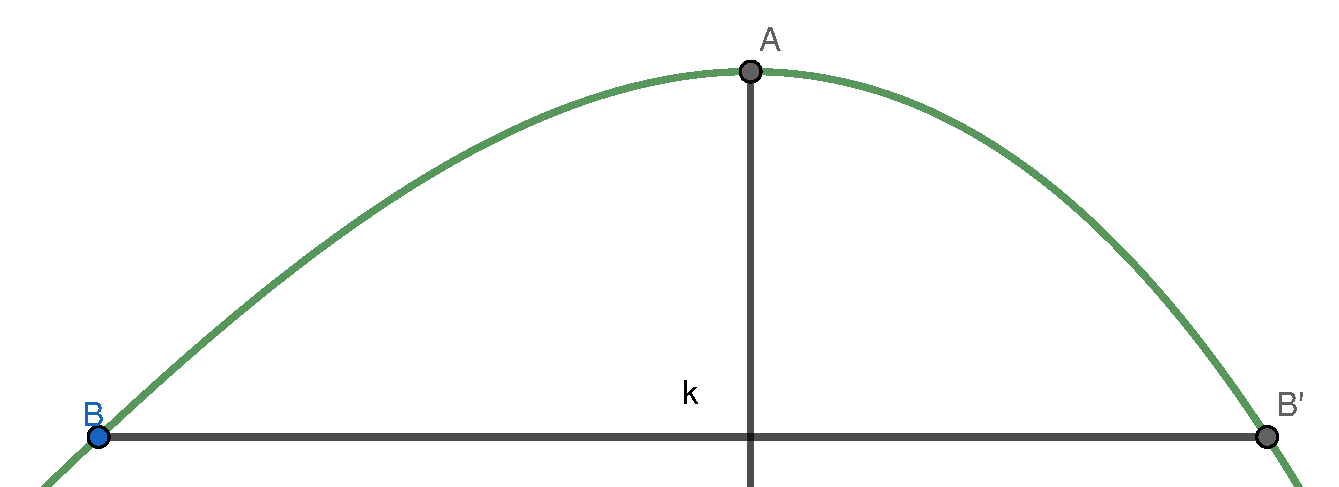
\includegraphics[scale=0.4]{Image/2019.pdf}
        \end{center}
        Ý tưởng của câu này là sẽ xét các đoạn xoay quanh điểm cực trị của $f(x)$ thì với $B < A$ thì luôn tồn tại $B' > A$ sao cho $f(B)  = f(B')$.
        
        
        Ta xét đoạn $[a,b]$ có $a < M < b$ và $c \in (a,M)$ bất kì. Nếu như $[a,b]$ có nhiều hơn một cực trị thì ta chỉ cần co thành đoạn $a' = a + \varepsilon_1 = $ và $b' = b - \varepsilon_2$, với $0 < \varepsilon_1, \varepsilon_2 < M$ đủ lớn sao cho $f'(x) = 0$ có duy nhất nghiệm trên $[a',b']$. Khi này ta xét đến đoạn $[a',b']$. 
        
        
        Không mất tính tổng quát, giả sử đoạn có 1 cực trị $M$ là $[a,b]$, và sẵn theo câu a) thì giả sử $M = max\{f(x)\}$ trên $[a,b]$
        
        
        Đặt $g(x) = f(x) - f(c)$ thì có $g(a) < 0$ và $ g(b) > 0$ thì $g(a).g(b) < 0$, rõ ràng là $g(x)$ có nghiệm trên $(a,b)$, tức là $\exists c' \in (a,b)\backslash{c}$ sao cho $f(c) = f(c')$. 


        Giả sử rằng $c' < M$ thì khi này ta có $f'(c) = f'(c')$, theo định lý Rolle tồn tại $d$ sao cho $f'(d) = 0$, mà $d < M$ vô lý, nên vì vậy $c' \in (M,b)$. 
        
        
        Tương tự như vậy mà vì $f$ liên tục nên có vô hạn $c \in (a,M)$ đồng thời cũng sinh ra vô hạn $c' \in (M,b)$


        Nếu với mỗi $c$ và $c'$ như vậy ta đặt $x_n = c$ và $y_n = c'$ thì sẽ có $f(x_n) = f(y_n)$ với mọi $n \geq 1$. Và ta sẽ xây dựng công thức tổng quát cho $x_n$ và $y_n$.


        Phân hoạch $[a,M]$ thành $n$ đoạn thì mỗi đoạn có độ dài là $\frac{M - a}{n}$,  và ta có dãy $x_1 = a, x_n = x_{n - 1}+ \frac{M - a}{2^n} $. Khi đó đường thẳng $y = f(x_n)$ nằm ngang trên đồ thị và cắt phần $f(x)$ đoạn $(M,b]$ tại một điểm duy nhất là $y_n$.
        
        Nếu $f(a) < f(b)$ thì ta cho $a$ tiến thêm một khoảng nữa là $a'$ sao cho $f(a') > f(b)$. Và giả sử $f(a) > f(b)$.


        Khi này nếu cho $n \to +\infty$ thì $\lim x_n = M$ thì đường thẳng $y$ cũng tịnh tiến lên trên về $(M,f(M))$, chứng tỏ rằng $(y_n)$ cũng tăng và bị chặn. Khi $y$ tiếp xúc $f(x)$ duy nhất tại điểm $(M,f(M))$ trên $[a,b]$ thì cũng là khi $\lim x_n = \lim y_n = M$, và ta hoàn tất chứng minh.
    \end{sol}
    \begin{bt}\vocab{(VMO 2020).}
        Cho dãy số $(x_n)$ xác định bởi: $x_1=1$ và $x_{n+1}=x_n+3\sqrt{x_n} + \frac{n}{\sqrt{x_n}}$,$\forall$n$\ge1$\\
a) Chứng minh rằng lim$\frac{n}{x_n}=0$\\ 
b) Tính lim$\frac{n^2}{x_n}$
    \end{bt}


    \begin{sol}
        a) Vì $x_n$ là dãy dương nên ta có $\frac{n}{x_n} > 0$. Dễ dàng chứng minh $x_n > n^2$ bằng quy nạp. Thì ta có $\frac{n}{x_n} < \frac{1}{n}$. Cho $n \to +\infty$ thì theo nguyên lý kẹp, $\lim\frac{n}{x_n} = 0$ 


        b) Vì $x_n > n^2$ nên $\lim x_n = +\infty$. Áp dụng định lý Stolz ta có 
        \[\lim \frac{n}{\sqrt{x_n}} =\lim \frac{1}{\sqrt{x_{n + 1}} - \sqrt{x_n}} = \lim \frac{\sqrt{x_{n+1}} + \sqrt{x_n}}{x_{n + 1} - x_n} = \lim \frac{\sqrt{x_n + 3\sqrt{x_n} + \frac{n}{\sqrt{x_n}}}+ \sqrt{x_n}}{3\sqrt{x_n} + \frac{n}{\sqrt{x_n}}} \]
        \[
            = \lim \frac{\sqrt{\sqrt{x_n} + \frac{3}{\sqrt{x_n}} + \frac{n}{x_n\sqrt{x_n}}}+ 1}{3 + \frac{n}{x_n}} = \frac{1 + 1}{3} = \frac{2}{3}
        \]
        Vì vậy $\lim\frac{n^2}{x_n} = \frac{4}{9}$
    \end{sol}

    \begin{bt}\vocab{(VMO 2021).}
        Cho dãy số $(x_n)$ xác định bởi $x_1\in (0;\frac{1}{2})$ và $x_{n+1}=3x_n^2-2nx_n^3, n\geq 1$.\\
        a) Chứng minh rằng $(x_n)$ hội tụ về $0$.

        
        b) Với mỗi $n\ge 1$, đặt $y_n=x_1+2x_2+\cdots+n x_n$. Chứng minh rằng $(y_n)$ có giới hạn hữu hạn.
    \end{bt}

    \begin{sol}
        a) Theo bất đẳng thức AM-GM ta có $$|x_{n + 1 }| = |\frac{x_n}{2n}.(2nx_n)\left(3 - 2nx_n\right)| \leq \frac{x_n}{2n}\left(\frac{3 - 2nx_n + 2nx_n}{2}\right)^2 \leq \frac{9}{16}|x_n|, \forall n\geq 2 $$
        Suy ra $|x_{n + 1}| \leq \left(\frac{9}{16}\right)^n x_1$. Chọn $n$ đủ lớn thì có $\lim x_n = 0$


        b) Theo tiêu chuẩn d'Alembert ta xét biểu thức 
        \[D =\lim\frac{(n + 1)x_{n+1}}{nx_n} \leq \lim \frac{9}{16}\frac{n + 1}{n} = \frac{9}{16}\]
        Vì $D < 1$ nên $y_n$ có giới hạn hữu hạn.
    \end{sol}
    \begin{bt}\vocab{(VMO 2022).}
        Cho $a$ là một số thực không âm và dãy số $(u_n)$ được định nghĩa như sau:
$$u_1=6, u_{n+1} = \frac{2n+a}{n} + \sqrt{\frac{n+a}{n}u_n+4}, \forall n \ge 1$$

Với $a \ge 0$, chứng minh rằng tồn tại giới hạn hữu hạn của $(u_n)$.
    \end{bt}

    \begin{sol}
        Dự đoán $\lim u_n = 5$. Bằng quy nạp ta chứng minh được $u_n \geq 5, \forall n \geq 1$. Ta có khai triển như sau:
        \[
            |u_n - 5| \leq |\frac{2n + a}{n} - 2| + |\sqrt{\frac{n+a}{n}u_n+4} -3| \leq \frac{a}{n} + \frac{\frac{n + a}{n}|u_n - 5| + \frac{5a}{n}}{\sqrt{\frac{ n+a}{n}u_n + 4} + 3}
        \]
        \[
            \leq \frac{n + a}{6n}|u_n - 5| + \frac{5a}{6n}
        \]  
        Vì $a$ là cố định nên ta chỉ cần xét từ $n \geq \lfloor a \rfloor $ là được. Ta có 
        \[|u_n - 5| \leq \frac{1}{3}|u_n -5| + y_n, \text{ với } \lim y_n = \lim \frac{5a}{6n} = 0\]
        Áp dụng bổ đề dãy số ta được $\lim x_n = 5$.
    \end{sol}
    %\vocab{Bình luận: } \textit{Bài toán này còn có một cách làm nữa đó là ta sử dụng giải tích tương tự bài dãy số năm 2017, việc trình bày cách 2 sẽ nhường lại cho bạn đọc.}
    \begin{bt}\vocab{(VMO 2023).}
        Xét dãy số $(a_n)$ thỏa mãn $a_1=\dfrac{1}{2}, a_{n+1}=\sqrt[3]{3a_{n+1}-a_n}$ và $0\le a_n\le 1, \forall n\ge 1.$

a. Chứng minh rằng dãy số $(a_n)$ được xác định duy nhất và có giới hạn hữu hạn.

b. Đặt $b_n=(1+2.a_1)(1+2^2a_2)...(1+2^na_n), \forall n\ge 1.$

Chứng minh rằng dãy số $(b_n)$ có giới hạn hữu hạn.
    \end{bt}

    \begin{sol}
        a) Đặt $a_n = 2\sin{\alpha_n}$. Ta có $\sin{\alpha_n} = 3\frac{a_{n + 1}}{2} - \frac{4a_{n + 1}^3}{2^3} \Rightarrow a_{n + 1} = 2\sin{\frac{\alpha_n}{3}}$
        

        Thực hiện truy toán như vậy nếu đặt $a_1 = 2\sin{\alpha}$ thì ta có $a_n = 2\sin{\frac{\alpha}{3^{n-1}}}$
        

        Do đó $(a_n)$ xác định duy nhất và $\lim a_n = 0$


        b) Ta có $\frac{b_{n + 1}}{b_n} = 1 + 2^na_n > 1$ nên $(b_n)$ tăng. Mặt khác, vì $0 < \frac{\alpha}{3^{n-1}} < \frac{\pi}{2}, \forall n \geq 1$.\\ Xét $f(x) = \sin{x} - x$ trên $(0, \frac{\pi}{2})$ có $f'(x) = \cos{x} - 1 \leq 0$ nên $f(x)$ giảm và $f(x) \leq 0$.\\ Do đó ta có đánh giá $$a_n =  2\sin{\frac{\alpha}{3^{n-1}}} \leq \frac{2\alpha}{3^{n-1}}$$
        Khi này viết lại với chú ý $\ln(x + 1) \leq x, \forall x \geq 1$
        \[
            b_n \leq  \prod_{i = 1}^n \left(1 + \frac{2^{i + 1}\alpha}{3^{i - 1}}\right)
            \Leftrightarrow \ln b_n \leq \sum _{i = 1}^n  \left(1 + \frac{2^{i + 1}\alpha}{3^{i - 1}}\right) \leq \sum_{i = 1}^n 6\alpha\frac{2^i}{3^i} = 12\alpha\left(1 - \left(\frac{2}{3}\right)^n\right) \leq 12\alpha
        \]
        Suy ra được $b_n \leq e^{12\alpha}$. Nên theo Weierstrass thì $(b_n)$ hội tụ, hoàn tất chứng minh.
    \end{sol}

    \begin{bt}\vocab{(VMO 2024).}
        Với mỗi số thực $x$, kí hiệu $\lfloor x \rfloor$ là số nguyên lớn nhất không vượt quá $x$.


Dãy số $\{a_n \}_{n=1}^{\infty}$ được định nghĩa bởi $a_n = \frac{1}{4^{\lfloor -\log_4 n \rfloor}}, \forall n \geq 1.$ Đặt $b_n = \frac{1}{n^2} \left( \sum_{k=1}^n a_k - \frac{1}{a_1+a_2} \right).$

a) Tìm đa thức $P(x)$ với hệ số thực sao cho $b_n = P \left( \frac{a_n}{n} \right), \forall n \geq 1$.\\
b) Chứng minh rằng tồn tại một dãy số tăng nghiêm ngặt $\{n_k \}_{k=1}^{\infty}$ của các số nguyên dương sao cho$$\lim_{k \to \infty} b_{n_k} = \frac{2024}{2025}.$$
    \end{bt}

    \begin{sol}
        a) Mỗi lần $n$ tăng gấp 4 lần thì $a_n$ cũng tăng gấp 4 lần, nếu không thì các số hạng kề $a_n$ không đổi. Vậy nên với mỗi $n$, $\exists t: 4^t \leq n \leq 4^{t + 1}$ và $a_n = 4^t$.\\
        Ta để ý rằng $a_1 = 1$, $a_2,a_3,a_4 = 4$, $a_5,a_6,...,a_{16} = 16$ và ta có lập luận rằng cứ mỗi $a_{4^{k-1} + 1},a_{4^{k-1} + 2},...,a_{4^k}$ thì giá trị vẫn giữ nguyên, và cứ một cụm như thế thì sẽ có tổng là $T_k = (4^{k} - (4^{k-1} + 1) + 1)4^k = 12.16^{k-1}$.


        Ta đặt $n = 4^m + r$ trong đó $m$ là số lớn nhất sao cho $4^m \leq n$ và $m,r \in \mathbb{Z}^+$. Tất nhiên là ta được $r = n - a_n$. Khi đó có 
        \[S = \sum_{i = 1}^{4^m + r} a_i = \sum_{i = 1}^{4^m}a_i + \sum_{i = 4^m + 1}^{4^m + r} a_n = 1 + \sum_{i = 0}^{m} T_i + a_n.r = 1 + \sum_{i = 0}^{m} 12.16^{i} + a_n(n - a_n)\]\[ = 1 + 4\frac{16^m - 1}{5}  + na_n - a_n^2 = 1 + \frac{4a_n^2 - 4}{5} +na_n -a_n^2 = -\frac{1}{5}a_n^2 + na_n + \frac{1}{5}\]
        Khi này thay $S$ vào $b_n$ ta được 
        \[b_n = \frac{1}{n^2}\left(S - \frac{1}{5}\right) = -\frac{1}{5}.\frac{a_n^2}{n^2} + \frac{a_n}{n} = P\left(\frac{a_n}{n}\right)\]
        Khi này ta có được $P(x) = -\frac{1}{5}x^2 + x$, hoàn tất câu a).


        b) Để giải quyết được câu b) thì ta hãy tìm hiểu một khái niệm khác trong \vocabf{tiền giải tích (Precalculus)} là \vocabf{Tập hợp trù mật}.

        
        \vocab{- Định nghĩa 9: } Một tập con $A$ trong $X$ được gọi \vocabf{trù mật (hoặc dày đặc)} trong $X$ nếu mọi điểm trong $X$ hoặc là thuộc $X$ hoặc gần tùy ý với một phần tử của $A$.


        Ta có một định lý khá quan trọng như sau:
        \begin{theo}[Định lý trù mật]
            -Với $a < b$ là hai số thực bất kì thì luôn tồn tại số hữu tỉ $q$ sao cho $a < q < b$.
        \end{theo}
        \vocab{Chứng minh: }Đặt $c = b - a > 0$. Khi đó tồn tại số nguyên dương $n$ sao cho $0 < \frac{1}{n} < c$. Điều này không phải hiển nhiên, ta có tiên đề sau
        \begin{theo}[Tiên đề Archimedes]
            -Cho $x,y$ là hai số thực dương, khi đó tồn tại số nguyên dương $m$ sao cho $mx > y$
        \end{theo}
        Cách chứng minh tiền đề này phải dùng đến \vocabf{lý thuyết topo} rất phức tạp nên ta hãy tạm thời thừa nhận nó mà không chứng minh lại.



        Chọn $x = c$ và $y = 1$ thì khẳng định trên đúng. Giờ ta xét các số hữu tỉ dạng $\frac{m}{n}$ với $m \in \mathbb{Z}$ và $n$ nguyên dương cố định. Cũng theo tiên đề Archimedes, luôn tồn tại số hữu tỉ $\frac{m_1}{n} < a$  và số hữu tỉ $\frac{m_2}{n} > b$


        Như vậy ta xét các số hữu tỉ $\frac{m_1}{n}, \frac{m_1 + 1}{n},...\frac{m_2 - 1}{n},\frac{m_2}{n}$. Đặt $p$ là số nguyên lớn nhất sao cho $\frac{p}{n} \leq a$. Khi đó có $a < \frac{p + 1}{n} < b$, hoàn tất chứng minh.


        Mở rộng sang ngôn ngữ dãy số thì điều này cho ta một hệ quả vô cùng quan trọng như sau: 
        \begin{theo}[Hệ quả 1]
            -Nếu $a < b$ là hai số thực dương thì tồn tại vô hạn số hữu tỉ thuộc $(a,b)$. Hay nói cách khác luôn tồn tại dãy $(s_n)$ hữu tỉ với $a < s_n < b, \forall n \geq 1$ và $\lim s_n = L$ với $L$ tùy ý thuộc $(a,b)$.
        \end{theo}
        Và ta còn có thể có một hệ quả thứ hai nữa là
        \begin{theo}[Hệ quả 2]
            -Nếu $(a_n)$ là dãy thực có các phần tử thuộc tập $T$ trù mật trên khoảng nào đó thì tồn tại một dãy $s_n$ nguyên dương tăng ngặt sao cho $\lim a_{s_n} = L$ với $L$ thuộc $T$ tùy ý.
        \end{theo}
        Quay trở lại bài toán, ta có $P(1) = \frac{4}{5} < \frac{2024}{2025} < P(2) = \frac{6}{5}$, cho nên vì tính liên tục của $P$ nên tồn tại $\alpha \in (1,2)$ sao cho $P(\alpha) = \frac{2024}{2025}$. Như vậy bài toán sẽ hoàn tất nếu ta chỉ ra được tập hợp 
        \[T = \left\{\frac{4^{i + 1}}{4^i + r} | i,r \in \mathbb{N}, 0 < q \leq 3.4^i\right\}\]
        trù mật trên $(1,2)$. Với $a < b \in (1,2)$ bất kì thì luôn tồn tại số $i,r$ sao cho $$ a < \frac{4^{i + 1}}{4^i + r} < b \Leftrightarrow \frac{a}{4^{i + 1}} < \frac{1}{4^i + r} < \frac{b}{4^{i + 1}} \Leftrightarrow 4^i(\frac{4}{b} - 1) < r < 4^i(\frac{4}{a} - 1) \Leftrightarrow 4^i(\frac{4}{a} - \frac{4}{b}) > 1$$  nếu chọn $i$ đủ lớn, dẫn tới sự tồn tại của $r$, vậy nên $T$ trù mật trên $(1,2)$. 

        
        
        Viết $n = 4^m + r$ thì ta được $\frac{a_n}{n} = \frac{4^{m + 1}}{4^m + r} \in T$. Theo hệ quả trù mật thì vì đã có $\left(\frac{a_n}{n}\right)$ là dãy hữu tỉ nên phải tồn tại dãy $(n_k)$ nguyên dương tăng ngặt để $\displaystyle \lim_{k \to +\infty}\frac{a_{n_k}}{n_k} = P(\alpha) = \frac{2024}{2025}$, hoàn tất chứng minh.
    \end{sol}
    \begin{bt}\vocab{(OLP 30/4 2024).}
        Cho dãy số $(x_n)$ được xác định bởi $$x_1 = 1, x_{n + 1} = \frac{1 + \sqrt{1 + x_n^2} - x_n}{1 + \sqrt{ 1 + x_n^2} + x_n}$$Chứng minh rằng $(x_n)$ có giới hạn hữu hạn và tìm giới hạn đó.
    \end{bt}

    \begin{sol}
        \vocab{Cách 1: Sử dụng bổ đề dãy số.} Viết lại ta có $x_{n + 1} = \sqrt{x_n^2 + 1} - x_n$. Dự đoán $\lim x_n = \frac{1}{\sqrt{3}}$. Lại có 
        $x_{n + 1} = \frac{1}{\sqrt{x_n^2 + 1} + x_n} > 0$ nên cũng có $x_{n+ 1} \leq 1$
        \[(x_{n + 1} - \frac{1}{\sqrt{3}}) = \sqrt{x_n^2 + 1} - \frac{2}{\sqrt{3}} - (x_n - \frac{1}{\sqrt{3}}) = \frac{(x_n + \frac{1}{\sqrt{3}})(x_n - \frac{1}{\sqrt{3}})}{\sqrt{x_n^2 + 1} + \frac{2}{\sqrt{3}}} \leq (\sqrt{3} - 1)(x_n - \frac{1}{\sqrt{3}})
        \]
        \[\Leftrightarrow |x_{n + 1} - \frac{1}{\sqrt{3}}| \leq (2 - \sqrt{3})|x_n - \frac{1}{\sqrt{3}}|\]
        Áp dụng bổ đề dãy số thì $(x_n)$ có giới hạn hữu hạn và $\lim x_n = \frac{1}{\sqrt{3}}$ 


        \vocab{Cách 2: Sử dụng lượng giác.} Đặt $x_n = \tan{x}$. Ta có 
        \[x_{ n + 1} = \sqrt{\tan^2{x} + 1} - tan{x} = \frac{1}{\cos x} - \tan{x} = \frac{\sin{\frac{\pi}{2}} - \sin{x}}{cos{x}} = \frac{2\cos(\frac{\pi}{4} + \frac{x}{2})\sin(\frac{\pi}{4} -\frac{x}{2})}{\sin(\frac{\pi}{2} - x)}\]
        \[
        = \frac{\cos(\frac{\pi}{4} + \frac{x}{2})}{\cos(\frac{\pi}{4} - \frac{x}{2})} = \tan(\frac{\pi}{4} - \frac{x}{2})
        \]
        Khi đó ta sẽ quy nạp được $x_n = \tan\left(\frac{\pi}{6} + \frac{\pi}{12}\left(-\frac{1}{2}\right)^{n - 1}\right)$. Vậy nên $\lim x_n = \frac{1}{\sqrt{3}}$
    \end{sol}
    \begin{bt}\vocab{(IMC 2015). }
    Cho hệ thức truy hồi được xác định bởi $F(0)=0$, $F(1)=\frac32$, và $F(n)=\frac{5}{2}F(n-1)-F(n-2)$
    for $n\ge2$.
    
    Chứng minh rằng $\displaystyle{\sum_{n=0}^{\infty}\,
        \frac{1}{F(2^n)}}$ là một số hữu tỉ.
    \end{bt}

    \begin{sol}
        Xét phương trình đặc trưng có $\lambda^2 - \frac{5}{2}\lambda + 1 = 0 \Leftrightarrow \lambda = 2$ hoặc $\lambda = \frac{1}{2}$, khi đó 
        \[
            F(n) = c_1.2^n + c_2. 2^{-n}
        \]
        Cho $n = 0$ và $n = 1$ rồi giải hệ phương trình, ta tìm được $c_1 = 1$ và $c_2 = -1$, do đó $F(n) = 2^n - 2^{-n}$. Đặt $x_n = 2^{2^n}$, khi đó ta được $F(2^n) = x_n - x_n^{-1}$. Mặt khác $x_{n + 1} = x_n^2$ nên
        \[
            \frac{1}{F(2^n)} = \frac{x_n}{x_n^2-1} = \frac{x_n+1}{x_n^2-1}-\frac{1}{x_n^2-1} = \frac{1}{x_n-1}-\frac{1}{x_{n+1}-1}.
        \]
        Khi đó tổng này hội tụ về $1$ là số hữu tỉ.
    \end{sol}

    \begin{bt}\vocab{(Đồng Tháp TST 2024). }
        Cho dãy số thực $(x_n)$ có $x_1 = 2$ và
        \[x_{n + 1} = \frac{n^2- 1}{x_n} + 2, \forall n \geq 1\]


        a) Chứng minh rằng $\lim x_n = +\infty$


        b) Xét dãy $(y_n)$ được xác định bởi
        \[y_n = \frac{x_1}{1.2^1} + \frac{x_2}{2.2^2} + \dots + \frac{x_n}{n.2^n}\]
        Chứng minh rằng $(y_n)$ có giới hạn hữu hạn và $\lim y_n < 2$.
        
    \end{bt}

    \begin{sol}
        a) Ta sẽ chứng minh quy nạp rằng $n \leq x_n \leq n + 1, \forall n \geq 1$. Với $x_1$ thì hiển nhiên đúng, giả sử mệnh đề đúng với $x_n$, ta có 
        \[x_{n + 1} \geq \frac{n^2 - 1}{n + 1} + 2 = n + 1\]
        \[x_{n + 1} \leq \frac{n^2 - 1}{n} + 2 = n - \frac{1}{n} +2 \leq n + 2\]
        Vậy nên mệnh đề quy nạp là đúng. Lại có $x_n \geq n$ nên $\lim x_n = +\infty$.


        b) Dễ thấy rằng $y_n$ là dãy tăng. Trước tiên ta xét chứng minh bxất đẳng thức sau đúng $ 2^{n - 1} > n, \forall n \geq 3$. Xét $f(x) = 2^{x - 1} - x$ trên $[3,+\infty)$ có $f'(x) = \ln2.2^{x - 1} - 1 > 0, \forall n \geq 3$. Vậy nên $f(x)$ tăng và $f(x) > f(3) = 1 > 0$ nên vì vậy $2^n > 2n, \forall n \geq 3$.
        
        
        Áp dụng đánh giá này đồng thời với $ 2^{n - 1} \geq n, \forall n < 3$, ta có 
        $$
        y_n = \sum_{i = 1}^n \frac{x_i}{i.2^i} \leq \sum_{i = 1}^n \frac{i + 1}{i.2^i} = 
        \sum_{i = 1}^n \frac{1}{2^i} + \frac{1}{i.2^i} < 1 - \frac{1}{2^{n}}+ \sum_{i = 1}^n \frac{1}{2i^2}
        $$
        Ta có đẳng thức tổng nghịch đảo bình phương là $\displaystyle \sum_{i = 1}^{\infty} \frac{1}{i^2} = \frac{\pi^2}{6}$, tương đương $\displaystyle \sum_{i = 1}^{n} \frac{1}{i^2} < \frac{\pi^2}{6}, \forall n \geq 1$ nên ta được
        \[y_n \leq 1 + \frac{\pi^2}{12} \]
        Suy ra $(y_n)$ bị chặn trên. Theo Weierstrass thì $(y_n)$ hội tụ và ta có được $\lim y_n \leq 1 + \frac{\pi^2}{12} < 2$
    \end{sol}

        \begin{sol}\vocab{Bình luận: } \textit{Trong bài toán trên thì ta đã sử dụng một đẳng thức rất nổi tiếng được Euler chứng minh khi ông 28 tuổi, ta phát biểu lại như sau:}


        \begin{theo}[Đẳng thức tổng nghịch đảo bình phương]
            -Cho $n$ là số thực dương lớn hơn 1, khi đó
            \[\sum_{i = 1}^{\infty} \frac{1}{i^2} = \frac{1}{1^2} + \frac{1}{2^2} + \frac{1}{3^2} + ... = \frac{\pi^2}{6}
            \]
        \end{theo}
        \textit{Để chứng minh đẳng thức này, ta sẽ sử dụng một khái niệm giải tích khác là Khai triển Taylor.}

        \begin{theo}[Khai triển Taylor]
            -Giả sử hàm số $f(x)$ có đạo hàm cấp tùy ý tại điểm $x_0$, khi này ta có 
            \[f(x) = f(x_0) + \frac{f'(x_0)}{1!} + \frac{f''(x_0)}{2!} + \frac{f'''(x_0)}{3!} + ... + \frac{f^{(n)}x_0}{n!} + ...= \sum_{i = 0}^{\infty} \frac{f^{(i)}(x_0)}{i!} \]
        \end{theo}
        \textit{Thông thường để thuận tiện thì ta xét khai triển tại điểm $x_0 = 0$, lúc này khai triển còn có tên gọi khác là Khai triển Maclaurin.}


        Quay trở lại bài toán, xét khai triển Maclaurin của $f(x) = \sin(x)$ như sau:
        \[
        f(x) = x - \frac{x^3}{3!} + \frac{x^5}{5!} - \frac{x^7}{7!} + ...\tag{1}
        \]
        Mặt khác, phương trình $\sin(x) = 0$ có các nghiệm là $\{0 , \pm \pi, \pm 2\pi,\pm 3\pi,...\}$, nên từ đó có
        \[\sin(x) = Cx(x^2 - \pi^2)(x^2 - 2^2\pi^2)(x^2 - 3^2\pi^2)... \tag{2}\]
        Từ (1) và (2) ta được   
        \[1 - \frac{x^2}{3!} + \frac{x^4}{5!} - \frac{x^6}{7!} + ... = C(x^2 - \pi^2)(x^2 - 2^2\pi^2)(x^2 - 3^2\pi^2)...
        \] Vì $C$ là hằng số tùy ý nên ta có 
        \[VP = (1 - \frac{x}{\pi^2})(1 - \frac{x}{2^2\pi^2})(1 - \frac{x}{3^2\pi^2})...\]
        Đồng nhất hệ số ta được
        \[-\frac{x}{3!} =-\frac{x}{\pi^2} -\frac{x}{2^2\pi^2} -\frac{x}{3^2\pi^2} -...\]
        \[\Leftrightarrow \frac{1}{1^2} + \frac{1}{2^2} + \frac{1}{3^2} + ... = \frac{\pi^2}{6}\]
    \end{sol}
        \begin{bt}\vocab{(TST Bắc Ninh 2018). }
            Cho dãy số $\left(x_n\right)$ được xác định bởi $$x_0=2017, x_n=-\frac{2017}{n} \sum_{k=0}^{n-1} x_k(n \geq 1)$$ Tìm giới hạn
\[
L=\lim \frac{n^2 \cdot\displaystyle \sum_{k=0}^{2017} 2^k x_k+5}{-2018 n^2+4 n-3} .
\]
        \end{bt}
        \begin{sol}
        Tương tự bài VMO 2011, chỉ xét riêng với $n \leq 2017$, ta có được
        \[
        x_{n} = -x_{n - 1} \frac{2018 - n}{n} = x_{n -2} \frac{(2018 - n)(2018 -(n - 1))}{n(n -1)} = ... = \frac{(-1)^nA_{2017}^{n - 1}}{n!} = (-1)^n \binom{2017}{n - 1}
        \]
        Khi đó 
        \[
            \displaystyle \sum_{i=0}^{2017} 2^k x_i = \displaystyle \sum_{i=0}^{2017} (-2)^i .1^{2017 - i}\binom{2017}{n - 1} = (1 - 2)^{2017} = -1
        \]
        Vì vậy $L = \frac{1}{2018}$
        \end{sol}
        \subsection{\LARGE \textcolor{dk}{Lời giải}}
    \newpage
    \thispagestyle{plain}
    
\includepdf[pages=1]{Image/bia/4.pdf}
    \section{\huge Bất đẳng thức}
    \subsection{\LARGE \textcolor{dk}{Đề bài}}
        \item \begin{btvn}\vocab{(Taiwan TST 2014).}
            Cho $a,b,c >0$. Chứng minh rằng
            \[
                3(a + b + c) \geq 8\sqrt[3]{abc} + \sqrt[3]{\frac{a^3 + b^3 + c^3}{3}}
            \]
        \end{btvn}
        \item \begin{btvn} Cho $a,b,c > 0$. Chứng minh rằng 
        \[
            \frac{a}{\sqrt{b + c}} + \frac{b}{\sqrt{c + a}} + \frac{c}{\sqrt{a + b}} \geq \sqrt{\frac{3}{2}(a + b + c)}
        \]
    \end{btvn}
        \item \begin{btvn}\vocab{(Japan MO 1997).}
            Cho $a,b,c >0$. Chứng minh rằng
            \[
                \frac{(b + c - a)^2}{a^2 + (b + c)^2} + \frac{(c + a - b)^2}{b^2 + (c + a)^2} + \frac{(a + b - c)^2}{c^2 + (a + b)^2} \geq \frac{3}{5}
            \]
        \end{btvn}
        \item \begin{btvn}\vocab{(IMO 2001).}
            Cho $a,b,c >0$. Chứng minh rằng
            \[
                \frac{a}{\sqrt{a^2 + 8bc}} + \frac{b}{\sqrt{b^2 + 8ca}} + \frac{c}{\sqrt{c^2 + 8ab}} \geq 1
            \]
        \end{btvn}
        \item \begin{btvn}\vocab{(IMO Shortlist 2009).}
            Cho $a,b,c >0$ thỏa mãn $\frac{1}{a} + \frac{1}{b} + \frac{1}{c} = a + b + c$
            \[
                \frac{1}{(2a + b + c)^2} + \frac{1}{(2b + c + a)^2} + \frac{1}{(2c + a + b)^2} \leq \frac{3}{16}
            \]
        \end{btvn}
        \item \begin{btvn}\vocab{(ELMOSL 2013).}
            Cho $a,b,c >0$ thỏa mãn $a + b + c = 3$. Chứng minh rằng
            \[
                \frac{18}{(3 -a )(4 - a)} + \frac{18}{(3 -b)(4 - b)} + \frac{18}{(3 -c )(4 - c)} + 2(ab + bc + ca) \geq 15
            \]
        \end{btvn}
        \item \begin{btvn}\vocab{(Canada MO 2002).}
            Cho $a,b,c >0$. Chứng minh rằng
            \[
                \frac{a^3}{bc} + \frac{b^3}{ca} + \frac{c^3}{ab} \geq a + b  +c
            \]
        \end{btvn}
        \item \begin{btvn}\vocab{(USAJMO 2012).}
            Cho $a,b,c >0$. Chứng minh rằng
            \[
                \frac{a^3 + 3b^3}{5a + b} + \frac{b^3 + 3c^3}{5b + c} + \frac{c^3 + 3a^3}{5c + a} \geq \frac{2}{3}(a^2 + b^2 + c^2)
            \]
        \end{btvn}
        \item \begin{btvn}\vocab{(IMO 2000).}
            Cho $a,b,c >0$ thỏa mãn $abc = 1$. Chứng minh rằng
            \[
                \left(a - 1 + \frac{1}{b}\right)\left(b - 1 + \frac{1}{c}\right)\left(c- 1 + \frac{1}{a}\right) \leq 1
            \]
        \end{btvn}
        \item \begin{btvn}\vocab{(ELMO 2003).}
            Cho $x,y,z > 1$ thỏa mãn $\frac{1}{x^2 - 1} + \frac{1}{y^2 - 1} + \frac{1}{z^2 - 1} = 1$. Chứng minh rằng
            \[
                \frac{1}{x + 1} + \frac{1}{y + 1} + \frac{1}{z + 1} \leq 1
            \]
        \end{btvn}
        \item \begin{btvn}\vocab{(USAMO 2003).}
            Cho $a,b,c >0$. Chứng minh rằng
            \[
                \frac{(2a + b + c)^2}{2a^2 + (b + c)^2} + \frac{(2b + c + a)^2}{2b^2 + (c + a)^2} + \frac{(2c + a + cb)^2}{2c^2 + (a + b)^2} \leq 9
            \]
        \end{btvn}
        \item \begin{btvn}\vocab{(USAMO 2017).}
            Cho $a,b,c,d \geq 0$ thỏa mãn $a + b + c + d = 4$. Tìm giá trị nhỏ nhất của
            \[
                \frac{a}{b^3 + 4} + \frac{b}{c^3 + 4} + \frac{c}{d^3 + 4} + \frac{d}{a^3 + 4}
            \]
        \end{btvn}

        \item \begin{btvn}\vocab{(USAMO 2004).}
            Cho $a,b,c >0$. Chứng minh rằng
            \[
                (a^5 - a^2 + 3)(b^5 - b^2 + 3)(c^5 - c^2 + 3) \geq (a + b + c)^3
            \]
        \end{btvn}
        \item \begin{btvn}\vocab{(TSTST 2012).}
            Cho $x,y,z >0$ thỏa mãn $xyz + xy + yz + zx  = x + y + z + 1$. Chứng minh rằng
            \[
                \frac{1}{3}\left(\sqrt{\frac{1 + x^2}{1 + x}} + \sqrt{\frac{1 + y^2}{1 + y}} + \sqrt{\frac{1 + z^2}{1 + z}}\right) \leq \left(\frac{x + y + z}{3}\right)^{5/8}
            \]
        \end{btvn}
        \item \begin{btvn}\vocab{(ELMO 2013).}
            Cho $a,b,c > 0$ thỏa mãn $a + b + c = \sqrt[7]{a} + \sqrt[7]{b} + \sqrt[7]{c}$. Chứng minh rằng $a^ab^bc^c \geq 1$.
        \end{btvn}
        \item\begin{btvn}
            Cho $a,b,c$ là độ dài 3 cạnh tam giác thỏa mãn $a^2 + b^2 + c^2 = 3$. Chứng minh rằng
            \[
                \frac{a}{\sqrt{b + c -a}} + \frac{b}{\sqrt{c + a -b}} + \frac{c}{\sqrt{a + b -c}} \geq 3
            \]
            
        \end{btvn}
        \begin{sol}
            Xét các biểu thức
            \[
                A =\sum_{cyc} \frac{a}{\sqrt{b + c -a}}, B = \sum_{cyc}a(b + c -a)
            \]
            Theo bất đẳng thức Holder ta có 
            \[A.A.B \geq (a + b + c)^3\]
            Ta cần chứng minh $(a + b + c)^3 \geq 9B \lra (a + b + c)^3 \geq 9\displaystyle \sum_{cyc}2ab - a^2$. Theo phép đặt $PQR$ tương tự bài trên ta có 
            \[p^3 \geq 9(2q - p^2 + 2q)
            \lra p^3 \geq 36q - 9p^2 \lra 9(p^2 -3q) + (p^3 - 9r) \geq 0
            \]
            Hiển nhiên đúng theo Schur. Vậy nên $A \geq 3$ và ta có điều phải chứng minh.
        \end{sol}
        \item\begin{btvn}
            Cho $a,b,c > 0$ có $abc = 1$. Chứng minh rằng
            \[
                \frac{a}{\sqrt{b + c + 7}} + \frac{b}{\sqrt{c + a + 7}} + \frac{c}{\sqrt{a + b + 7}} \geq 1
            \]
        \end{btvn}
        \begin{sol}
            Xét các biểu thức 
            \[
                A = \sum_{cyc}\frac{a}{\sqrt{b + c + 7}}, B = \sum_{cyc} a(b + c + 7) = \sum_{cyc} 2bc + 7a
            \]
            Theo bất đẳng thức Holder ta có 
            \[
                A^2B \geq (a + b + c)^3
            \]
            Ta cần chứng minh
            \[
                (a + b + c)^3 \geq \sum_{cyc}2bc + 7a
            \]
            Theo phép đặt PQR ta được
            \[
                p^3 \geq 2q + 7p \lra p^3 - 2q - 7p \geq 0
            \]
            Ta có $VT \geq p^3 -\frac{2}{3}p^2 - 3p = p(p^2 - \frac{2}{3}p - 3) \geq 0$ vì $p^3 \geq 27r \lra p \geq 3$. Vậy nên $A \geq 1$ và ta có điều phải chứng minh.
        \end{sol}
        \item\begin{btvn}
            Cho $a,b,c \geq 0$ thỏa mãn $ab + bc + ca > 0$. Chứng minh rằng
            \[\sqrt{\frac{a}{b + c}} + \sqrt{\frac{b}{c + a}}+ \sqrt{\frac{c}{a+ b}} \geq 2
            \]
        \end{btvn}
        \begin{sol}
            Xét các biểu thức
            \[
                A = \sum_{cyc} \sqrt{\frac{a}{b + c}},
                B = \sum_{cyc} a^2( b + c)
            \]
            Áp dụng bất đẳng thức Holder, ta có
            \[
                A.A.B \geq (a + b + c)^3
            \]
            Ta cần chứng minh $(a + b + c)^3 \geq 4B$. Theo phép đặt PQR, ta có
            \[
                p^3 \geq 4(pq - 3r) \lra (p^3 - 4pq + 9r) + 3r \geq 0
            \]
            Điều này luôn đúng theo bất đẳng thức Schur, hoàn tất bài toán.
        \end{sol}
    
        \item\begin{btvn}
            Cho $a,b,c > 0$ thỏa mãn $a^2 + b^2 + c^2 = a + b + c$. Chứng minh rằng 
            \[
                a^2b^2 + b^2c^2 + c^2a^2 \leq ab + bc + ca
            \]
        \end{btvn}
        \begin{sol}
            Ta có 
            \[
                (a^2 + b^2 + c^2)^2 = (a + b + c)^2 \lra \sum_{cyc}a^4 + 2b^2c^2 = \sum_{cyc}a^2 + 2bc
            \]
            Vậy nên ta cần chứng minh $a^4 + b^4 + c^4 \geq a^2 + b^2 + c^2$. Áp dụng bất đẳng thức Holder ta được
            \[
                (a^4 + b^4 + c^4)(a + b + c)^2 \geq (a^2 + b^2 + c^2)^3 \lra a^4 + b^4 + c^4
            \]
            Hoàn tất bài toán.
        \end{sol}
        
    
    
        \item\begin{btvn}
            Cho $a,b,c > 0$. Chứng minh rằng
            \[\sqrt{\frac{a + b}{c}} + \sqrt{\frac{b + c}{a}} + \sqrt{\frac{c + a}{b}} \geq 4(a +b + c)\sqrt{\frac{a + b + c}{3(a + b)(b + c)(c + a)}}
            \]
        \end{btvn}
        \begin{sol}
        Sử dụng bất đẳng thức Holder ta có 
            \[
                \left(\sum_{cyc}c(a+b)^2\right)\left(\sqrt{\frac{a + b}{c}} + \sqrt{\frac{b + c}{a}} + \sqrt{\frac{c + a}{b}}\right)^2 \geq 8(a + b +c)^3
            \]
            Ta cần chứng minh 
            \[
                    8(a + b + c)^3 \geq 16\frac{(a + b + c)^3}{3(a + b)(b + c)(c + a)} \left(\sum_{cyc}c(a+b)^2\right)
            \]
            \[
                \lra 3(a + b)(b + c)(c + a) \geq 2 \left(\sum_{cyc}c(a+b)^2\right)
            \]
            Chuẩn hóa $a + b + c = 3$, ta có 
            \[
                3(3 - a)(3 - b)(3 - c) \geq 2\left(\sum_{cyc}a(3-a)^2\right) = 2\sum_{cyc}a^3 - 6a^2 + 9a \tag{1}
            \]
            Theo phép đặt PQR, ta có các biểu thức sau:
                \begin{align*}
                    &(3 - a)(3 - b)(3 - c) = 3q - r\\
                    &a^2 + b^2 + c^2 = 9 -2q\\
                    &a^3 + b^3 + c^3 = p^3 - 3pq + 3r = 27 - 9q + 3r
                \end{align*}
                Từ đó ta được
            \[
                (1) \lra 9q - 3r \geq 2(27 - 9q + 3r - 54 + 12q +27) = 2(3q +3r) \lra q \geq 3r
            \]
            bất đẳng thức này luôn đúng vì $ r \leq \frac{pq}{9} \lra q \geq 3r$. Từ đó cho ta điều phải chứng minh.
            \end{sol}
            \item\begin{btvn}
                Cho $a,b,c > 0$ có $a + b + c = 1$. Chứng minh rằng
                \[
                    \frac{a}{\sqrt{b + c}} + \frac{b}{\sqrt{c + a}} + \frac{c}{\sqrt{a + b}} \geq \sqrt{\frac{3}{2}}
                \]
            \end{btvn}
            \begin{sol}
                Sử dụng bất đẳng thức Holder ta được
                \[
                    \left(\sum_{cyc}a^2(b + c)\right)\left(\sum_{cyc}\frac{a}{\sqrt{b + c}}\right)^2 \geq (a + b + c)^3
                \]
                Ta cần chứng minh 
                \[
                    (a + b + c)^3 \geq  \frac{3}{2}\left(\sum_{cyc}a^2(b + c)\right) \lra 2 \geq 3\sum_{cyc}a^2(1 -a) = 3(q - 3r) \lra 3q \leq 9r + 2
                \]
                Lại có $9r \leq q$ nên tương đương $3q \leq 9r + 2 \leq q + 2 \lra q \leq 1$. Điều này rõ ràng đúng, nên từ đó cho ta điều phải chứng minh.
            \end{sol}
            \item\begin{btvn}
                Cho $a,b,c > 0$ có $a + b + c = 1$. Chứng minh rằng
                \[
                    4abc\left[\frac{a}{(a + 1)^2} + \frac{b}{(b + 1)^2} + \frac{c}{(c + 1)^2}\right] + 1 \geq \frac{13}{4}(ab + bc + ca)
                \]
            \end{btvn}
            \begin{sol}
                Ta sẽ cần chứng minh 2 bất đẳng thức nhỏ sau:
                \[
                \left\{
                    \begin{array}{l}
                        (a + b + c)^2 \geq 3(ab + bc + ca)\\
                        \frac{a}{(a + 1)^2} + \frac{b}{(b + 1)^2} + \frac{c}{(c + 1)^2}\geq \frac{1}{16}\left(\frac{1}{a} + \frac{1}{b} + \frac{1}{c}\right)
                    \end{array}
                \right.\]
                bất đẳng thức thứ nhất hiển nhiên đúng theo bất đẳng thức Schur. Ta quan tâm đến bất đẳng thức thứ 2. Sử dụng bất đẳng thức Holder ta có 
                \[
                    \left(\sum_{cyc}a(a + 1)\right)^2\left[\frac{a}{(a + 1)^2} + \frac{b}{(b + 1)^2} + \frac{c}{(c + 1)^2}\right] \geq (a + b + c)^3
                \]
                Ta cần chứng minh $\displaystyle (a + b + c)^3 \geq \frac{1}{16}\left(\sum_{cyc}a(a + 1)\right)^2\left(\frac{1}{a} + \frac{1}{b} + \frac{1}{c}\right)$. Theo phép thế PQR ta có
                \[
                    1 \geq \frac{q^2}{4}.\frac{q}{r} \lra 4r \geq q^3
                \]
                Thật vậy ta có $r \geq \frac{4q - 1}{9}$ nên ta sẽ cần đánh giá 
                $9q^3 - 4q + 1 \leq 0$. Xét $f(q) = 9q^3 - 4q + 1$ trên $[0,\frac{1}{3}]$. Ta có $f'(q) = 27q^2 - 4 \leq \frac{1}{3} - 4 < 0$ nên $f(p)$ giảm.
    
    
                Suy ra $f(p) \leq f(\frac{1}{3}) = 0$ nên từ đó $f(p) \leq 0, \forall q \leq \frac{1}{3}$, vậy nên bất đẳng thức thứ hai cũng đúng.
    
    
                Ta lấy bất đẳng thức thứ hai nhân cho $4abc$ và cộng với bất đẳng thức thứ nhất thì có điều phải chứng minh.
                
            \end{sol}
            \item\begin{btvn}
                Cho $a,b,c > 0$ thỏa mãn $a + b + c = \frac{1}{a} + \frac{1}{b} + \frac{1}{c}$. Chứng minh rằng
                \[
                    \sqrt[3]{7a^2b + 1} + \sqrt[3]{7b^2c + 1} + \sqrt[3]{7c^2a + 1} \leq 2(a + b + c)
                \]
            \end{btvn}
            \item\begin{btvn}\vocab{(Võ Quốc Bá Cẩn). }
                Cho $a,b,c \geq 0$ thỏa mãn $a + b + c = 1$. Chứng minh rằng
                \[
                    \frac{1}{\sqrt{4a + 5b^2}} + \frac{1}{\sqrt{4b + 5c^2}} + \frac{1}{\sqrt{4c + 5a^2}} \leq \frac{3}{\sqrt{17}}
                \]
            \end{btvn}
            \item\begin{btvn}\vocab{(KHTN 2020). }Cho $a,b,c > 0$ thỏa mãn $a + b + c = 3$. Chứng minh rằng
                \[
                    3\left(\frac{1}{a} + \frac{1}{b} + \frac{1}{c} - 1\right)^2 + 1 \geq \frac{4}{abc} + 3\left(\frac{a}{bc} +  \frac{b}{ca} + \frac{c}{ab}\right)
                \]
            \end{btvn}
            \item\begin{btvn}
                Cho các số thực $a,b,c$. Chứng minh rằng
                \[
                    a(a + b)^3 + b(b + c)^3 + c(c +a)^3 \geq \frac{8}{27}(a + b + c)^4
                \]
            \end{btvn}
            \item\begin{btvn}
                Cho $a,b,c \geq 0$ không có 2 số nào đồng thời bằng 0. Chứng minh rằng 
                \[
                    \sqrt{\frac{a}{b +c }} + \sqrt{\frac{b}{ c +a }} + \sqrt{\frac{c}{a + c}} \leq \frac{3}{\sqrt{2}}
                \]
            \end{btvn}
            \item\begin{btvn}
                Cho $a,b,c \geq 0$ không có 2 số nào đồng thời bằng 0. Chứng minh rằng
                \[
                    \frac{a^2 - bc}{2b^2 - 3bc + 2c^2} + \frac{b^2 - ca}{2c^2 - 3ca + 2a^2} + \frac{c^2 - ab}{2a^2 - 3ab + 2b^2} \geq 0
                \]
            \end{btvn}
            \item\begin{btvn}
                Cho $a,b,c \geq 0$ thỏa mãn $a^2 + b^2 + c^2 = 1$. Chứng minh rằng
                \[
                    \frac{bc}{a^2 + 1} + \frac{ca}{b^2 + 1} + \frac{ab}{c^2 + 1} \leq \frac{3}{4}
                \]
            \end{btvn}
            \item\begin{btvn}\vocab{(Vasile Cirtoaje). }
                Cho $a, b, c \geq 0$ không có 2 số nào đồng thời bằng $0$. Chứng minh rằng
                \[
                    \frac{1}{5a^2 - ab + 5b^2} + \frac{1}{5b^2 - bc + 5c^2} + \frac{1}{5c^2 - ca + 5a^2} \geq \frac{1}{a^2 + b^2 + c^2}
                \]
            \end{btvn}
            \item \begin{btvn}
                Cho $a,b,c \geq 0$ không có hai số nào đồng thời bằng $0$. Chứng minh rằng
                \[
                    \frac{1}{a^2 + bc} + \frac{1}{b^2 + ca} + \frac{1}{c^2 + ab} \geq \frac{3(a + b + c)^2}{2(a^2 + b^2 + c^2)(ab + bc + ca)}
                \]
            \end{btvn}
            \item\begin{btvn}\vocab{(Phạm Kim Hùng). }
                Cho $a,b,c$ là độ dài 3 cạnh tam giác. Chứng minh rằng
                \[
                    \frac{a}{b + c} + \frac{b}{c + a} + \frac{c}{a + b} + \frac{ab + bc + ca}{a^2 + b^2 + c^2} \leq \frac{5}{2}
                \]
            \end{btvn}

            \item\begin{btvn}
                Cho các số $a,b,c \geq \frac{1}{2}$ thỏa mãn $abc = 1$. Chứng minh rằng
                \[
                    \frac{1}{a + 2b} + \frac{1}{b + 2c} + \frac{1}{c + 2a} \leq 1
                \]
            \end{btvn}
            
        \item \begin{btvn}\vocab{(VMO 2014).} Cho $x,y,z >0$. Tìm giá trị lớn nhất của
        \[P=\frac{x^3y^4z^3}{(x^4+y^4)(xy+z^2)^3}+\frac{y^3z^4x^3}{(y^4+z^4)(yz+x^2)^3}+\frac{z^3x^4y^3}{(z^4+x^4)(zx+y^2)^3}\]
        \end{btvn}
        \item \begin{btvn}\vocab{(VMO 2015).} Cho $a,b,c \geq 0$. Chứng minh rằng
            \[{ 3(a^2+b^2+c^2) \geq (a+b+c)(\sqrt{ab}+\sqrt{bc}+\sqrt{ca})+(a-b)^2+(b-c)^2+(c-a)^2 \geq (a+b+c)^2}\]
            
        \end{btvn}
        \item \begin{btvn}\vocab{(VMO 2020).} Cho các ý sau:
        
            (a) Cho $a,b,c \in \bb{R}$ và $a^2 + b^2 + c^2 = 1$. Chứng minh rằng
            \[
                |a - b| + |b - c| + |c - a| \leq 2\sqrt{2}
            \]
    
            (b) CHo $a_1, a_2,\dots,a_{2019} \in \bb{R}$ và $\dsum_{i = 1}^{2019}a_i^2 = 1$. Tìm giá trị lớn nhất của 
            \[
                S = |a_1 - a_2| + |a_2 - a_3| + \dots + |a_{2019} - a_1|
            \]
            \end{btvn}
        \item \begin{btvn}\vocab{(VMO 2023).}
            Cho $a,b,c > 0$ thỏa mãn $a^2 + b^2 + c^2 = 2(ab + bc + ca)$. Tìm giá trị lớn nhất của $k$ sao cho bất đẳng thức sau đây đúng:
            \[
                \frac{1}{kab + c^2} + \frac{1}{kbc + a^2} + \frac{1}{kca + b^2} \geq \frac{k + 3}{a^2 + b^2 + c^2}
            \]
        \end{btvn}
        \subsection{\LARGE \textcolor{dk}{Lời giải}}
        
        \newpage
        \thispagestyle{plain}
        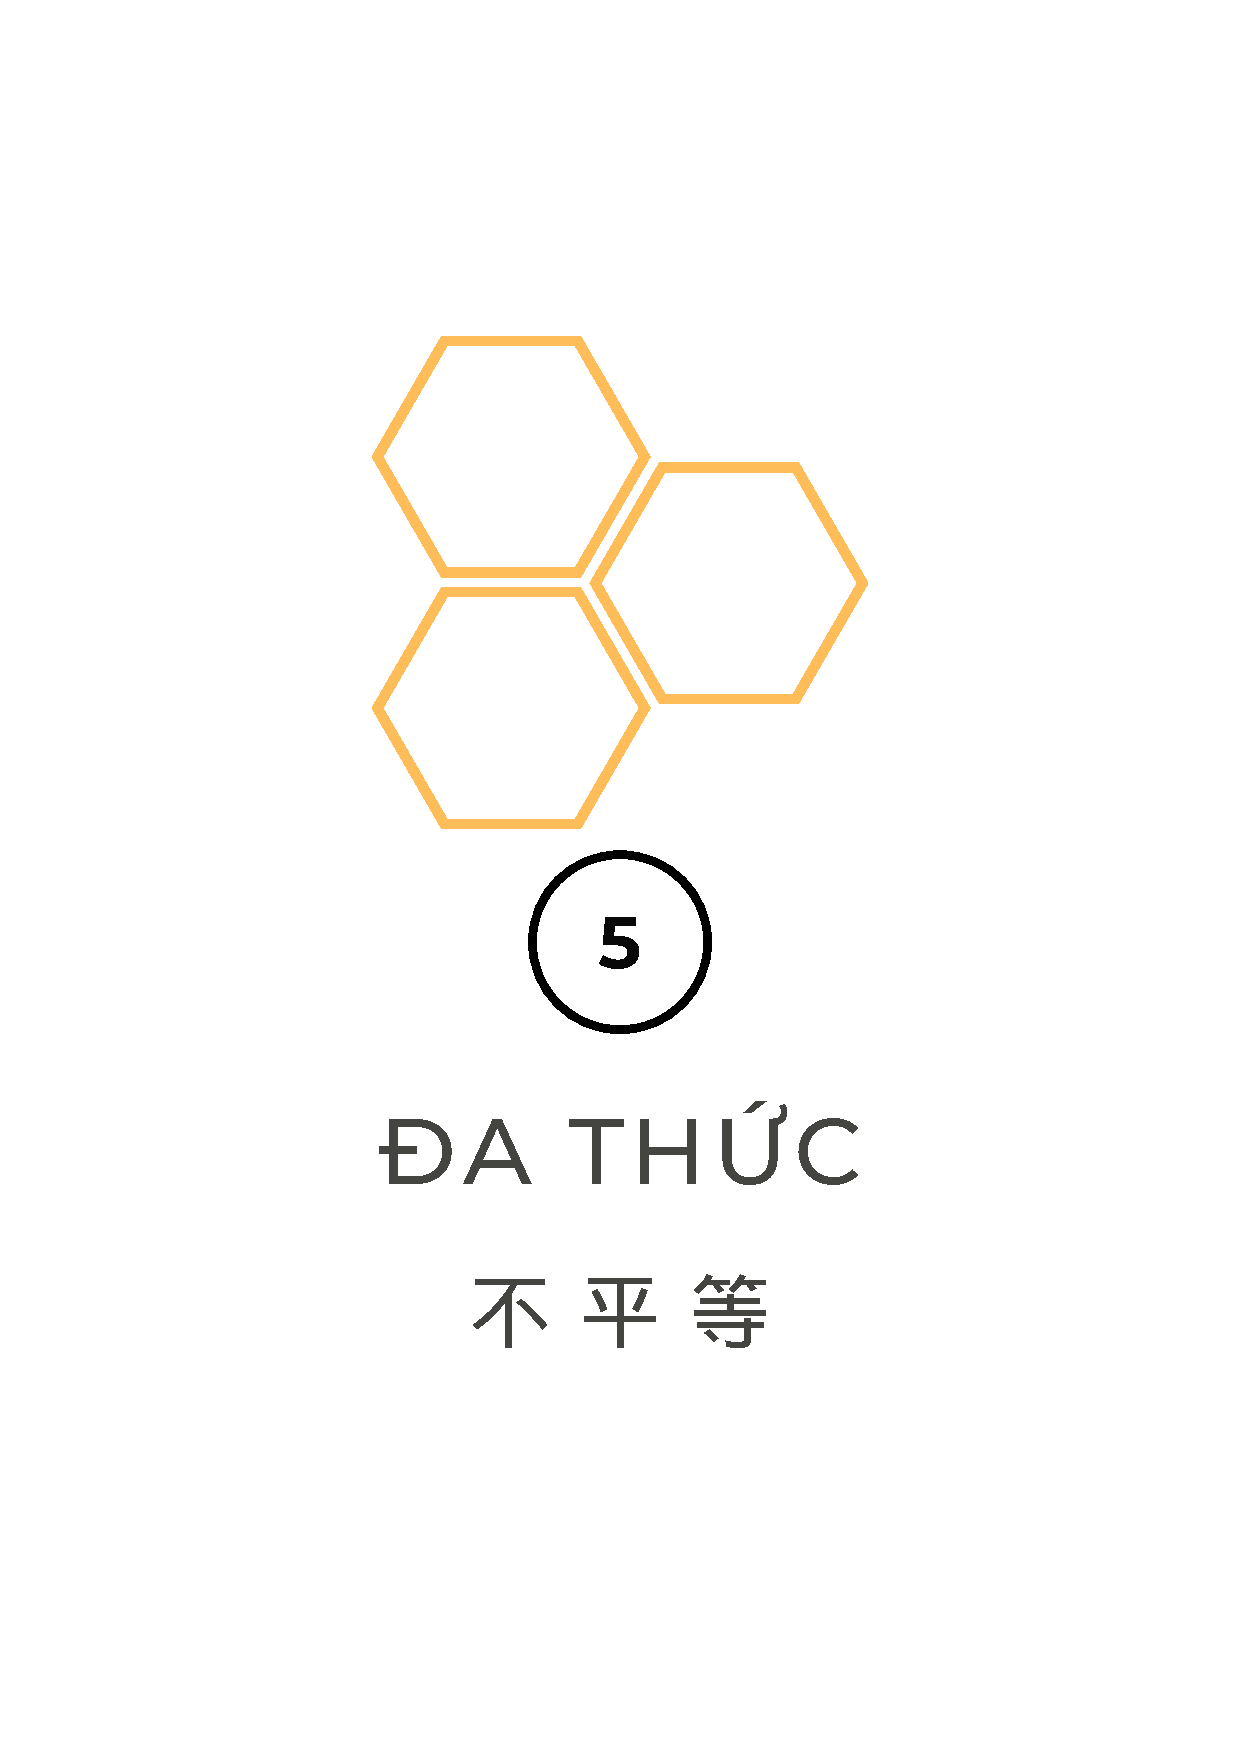
\includepdf[pages=1]{Image/bia/5.pdf}
        \section{\huge Đa thức}
        \subsection{\LARGE \textcolor{dk}{Đề bài}}
        \item \begin{btvn}\vocab{(Bulgaria TST 2015).}
            Tìm tất cả các đa thức hệ số thực $f(x) = \dsum_{i = 1}^{2n}$ có $2n$ nghiệm thực sao cho $|a_i| \leq 2$ với mọi $i = 1,2,\dots,n$
        \end{btvn}
        \item \begin{btvn}\vocab{(Romania TST 1990).}
            Cho $a \in \bb{Z}\backslash \{0\}$. Chứng minh rằng đa thức
            \[
                P(x) = x^n + ax^{n - 1} + \dots + ax - 1
            \]
            bất khả quy trên $Z[x]$.
        \end{btvn}
        \item \begin{btvn}\vocab{(Romania TST 1997).} Cho số nguyên $n \geq 2$ và đa thức
        \[
            P(x) = x^n + a_{n - 1}x^{n - 1} +\dots + a_1x+1
        \]
        là đa thức hệ số nguyên dương sao cho $a_k = a_{n - k}$ với mọi $k \in [n - 1]$. Chứng minh rằng tồn tại vô hạn cặp cặp số nguyên $(x,y)$ sao cho $x \mid P(y)$ và $y \mid P(x)$.
        \end{btvn}
        \item \begin{btvn}\vocab{(ITAMO 1994).}
            Cho đa thức $P(x) = a_0 + a_1x + \dots + a_{2n}x^{2n}$ là khai triển của biểu thức $(1 + x + x^2)^n$. Tính
            \begin{enumerate}[label=(\alph*)]
                \item $a_0 + a_2 + \dots + a_{2n}$
                \item $a_1 + a_3 + \dots + a_{2n - 1}$
                \item $a_0a_1 - a_1a_2 + a_2a_3 -\dots- a_{2n - 1}a_{2n}$
            \end{enumerate}
        \end{btvn}
        \item \begin{btvn}
            Cho $P(x) = a_nx^n + \dots + a_0$ là đa thức không âm với hệ số phức. Chúng ta nói rằng $P(x)$ là \textit{tương hỗ} nếu như $a_k = a_{n - k}$ với mọi $k \in \{0,1,\dots,n\}$ hoặc $a_k = -a_{n - k}$ với mọi $k \in \{0,1,\dots,n\}$. Với mỗi đa thức ta ký hiệu $[P(x)]$ như sau: 
            \begin{enumerate}
                \item $[P(x)] = 1$ nếu như $a_k = a_{n - k}$ với mọi $k \in \{0,1,\dots,n\}$
                \item $[P(x)] = -1$ nếu như $a_k = -a_{n - k}$ với mọi $k \in \{0,1,\dots,n\}$
            \end{enumerate}
            \begin{enumerate}[label=(\alph*)]
                \item Chứng minh rằng nếu như $P(x)$ và $Q(x)$ là \textit{tương hỗ} thì $P(Q(x))$ cũng tương hỗ và $[P(Q(x))] = [P(x)][Q(x)]$
                \item Chứng minh rằng nếu như $P(x)$ và $P(Q(x))$ là \textit{tương hỗ} thì $Q(x)$ là \textit{tương hỗ} và $[Q(x)] = \frac{[P(Q(x))]}{[P(x)]}$
            \end{enumerate}
        \end{btvn} 
        \item \begin{btvn} Cho đa thức monic $f(x) = \dsum_{i = 0}^n a_ix^i$ có các nghiệm thực $x_1,\dots,x_n$ thuộc đoạn $[-1,1]$ và hệ số thỏa mãn $a_{n - i} = a_i$, $i = 0,1,\dots,n$. Chứng minh rằng $f(x) = (x + 1)^p(x - 1)^{2q}$ với $p,q \in \bb{N}$ và $p + 2q = n$.
        \end{btvn}
        \item \begin{btvn}\vocab{(Romania MO).} Cho đa thức $P(x) = a_{2n}x^{2n} + a_{2n - 1}x^{2n - 1} +\dots + a_0$ sao cho $a_k = a_{2n - k}$ với $k = 0,1,\dots,n$
        \begin{enumerate}[label=(\alph*)]
            \item Chứng minh rằng tồn tại một đa thức $Q$ sao cho 
            \[  
                P(x) = x^nQ\left(x + \frac{1}{x}\right)
            \]
            \item Nếu $a_0 = a_{2n} = 1$ và $|a_{n}| < 2$. Chứng minh rằng $P(x)$ có ít nhất một nghiệm phức.
        \end{enumerate}
        \end{btvn}
        \item \begin{btvn}
            Cho đa thức $P(x) = a_dx^d + \dots + a_1 x + a_0$ và định nghĩa
            \[
                C(P(x)) = a_d^2 + a_{d - 1}^2 + ... + a_1^2 + a_0^2
            \]
            Cho $P(x) = 3x^2 + 7x + 2$. Tìm đa thức $Q(x)$ hệ số thực sao cho $Q(x) = 1$ và $C((P(x))^n) = C((Q(x))^n)$ với mọi số nguyên dương $n$.
        \end{btvn}
        \item \begin{btvn}\vocab{(VMO 1998).}
            Tìm tất cả các số nguyên dương $n$ sao cho tồn tại một đa thức $P(x)$ với hệ số thực thỏa mãn $P(x^{1998} - x^{-1998}) = x^n - x^{-n}$
        \end{btvn}
        \item \begin{btvn}
            Cho $n \equiv 0,1 \pmod{3}$. Chứng minh rằng đa thức $P(x) = x^n + x + 1$ bất khả quy trên $Z[x]$.
        \end{btvn}
        \item \begin{btvn}\vocab{(USA TST 2014).} Cho $n$ là số nguyên dương chẵn. Đặt $c_1,c_2,\dots,c_n$ là các số thực sao cho 
        \[
            \sum_{i = 1}^n |c_i - 1| < 1
        \]
        Chứng minh rằng đa thức 
        \[
            P(x) = 2x^n - c_{n - 1}x^{n - 1} + c_{n - 2}x^{n -2} -\dots-c_1x + 2
        \]
        không có nghiệm thực.
        \end{btvn}
        \item \begin{btvn}
            Cho $a_1,a_2,\dots,a_n$ là các số phức có module $r > 0$. Gọi $T_s$ là tổng của tích bất kì $s$ số từ $a_1,\dots,a_n$. Giả sử $T_{n - s} \neq 0$. Chứng minh rằng $\left|\frac{T_s}{T_{n - s}}\right| = r^{2s - n}$.
        \end{btvn}
        \item \begin{btvn}
            Cho đa thức $P(x) = b_dx^d + \dots + b_0$, chúng ta định nghĩa tổng $BB$ của $P(x)$ là $b_0b_1 + b_1b_2 +\dots+b_{d - 1}b_d$. Xác định rằng tồn tại hay không số thực $r$ và $s$ sao cho với mỗi số nguyên dương $k$, tổng $BB$ của $(x^2 + rs + s)^k$ bằng tổng $BB$ của $(2x^2 + 7x + 3)^k$.
        \end{btvn}
        \item \begin{btvn}
            Cho đa thức $P(x) = x^d + a_{d - 1}x^{ d- 1} + \dots + a_1x + a_0$ là đa thức có bậc $d \geq 3$ với hệ số nguyên sao cho $a_k + a_{d -k}$ là số chẵn với $k \in [d- 1]$ và $a_0$ cũng là số chẵn. Nếu như $P(x) = Q(x)R(x)$ trong đó $R(x)$ và $Q(x)$ là đa thức khác hằng hệ số nguyên và $\deg Q(x) \leq \deg R(x)$ với tất cả các hệ số của $R(x)$ đều lẻ. Chứng minh rằng $P(x)$ có ít nhất một nghiệm nguyên.
        \end{btvn}
        \item \begin{btvn}
            Cho $a \neq 0,b,c$ là các số thực. Chứng minh rằng tồn tại một đa thức hệ số thực $P(x)$ sao cho $x^2 + 1 \mid aP(x)^2 + bP(x) + c$.
        \end{btvn}
        \item \begin{btvn}
            Với $k,m,n$ là số nguyên không âm. Chứng minh rằng
            \[
                x^2 + x + 1 \mid x^{3k + 2} + x^{3m + 1} + x^{3n}
            \]
        \end{btvn}
        \item \begin{btvn}\vocab{(Poland MO 1986).}
            Chứng minh rằng với mỗi số nguyên dương $k$ ta luôn có
            \[
                x^5 + 1 \mid (x^4 - 1)(x^3 - x^2 + x - 1)^k + (x + 1)x^{4k - 1}
            \]
        \end{btvn}
        \item \begin{btvn}\vocab{(Poland MO 1988).}
            Cho đa thức $f(x)$ và $n$ là số nguyên dương. Chứng minh rằng nếu $f(x^n)$ chia hết cho $x - 1$ thế thì cũng chia hết cho
            \[
                x_{n - 1} + x_{n - 2} +\dots + x + 1
            \]
        \end{btvn}
        \item \begin{btvn}\vocab{(Poland MO 1996).}
            Tìm tất cả các cặp $(n,r) \in \bb{N} \times \bb{R}$ sao cho đa thức $(x + 1)^n - r$ chia hết cho $2x^2 + 2x + 1$.
        \end{btvn}
        \item \begin{btvn}
            Cho số thực $|a| \leq 1$. Chứng minh rằng tất cả các nghiệm của đa thức $x^{n + 1} -ax^n -ax + 1 = 0$ đều nằm trên đường tròn đơn vị.
        \end{btvn}
        \item \begin{btvn}\vocab{(USAMO 2014).}
            Cho các số thực $a,b,c,d$ thỏa mãn $b - d \geq 5$ và các nghiệm $x_1,x_2,x_3$ và $x_4$ của đa thức $P(x) = x^4 +ax^3 + bx^2 + cx + d$ là số thực. Tìm giá trị nhỏ nhất của
            \[
                (x_1^2 + 1)(x_2^2 + 1)(x_3^2 + 1)(x_4^2 + 1)
            \]
        \end{btvn}
        \item \begin{btvn}\vocab{(Mongolian MO 2018).}
            Tìm tất cả các đa thức $P(x)$ sao cho với mọi số thực $x,y,z$ thỏa mãn $x + y + z = 0$, ba điểm $(x,P(x)), (y,P(y)),(z,P(z))$ thẳng hàng trên mặt phẳng tọa độ.
        \end{btvn}

        \item \begin{btvn}\vocab{(Canada MO 2018).}
            Tìm tất cả các đa thức $P(x)$ hệ số thực thỏa mãn tính chất: tồn tại một đa thực hệ số thực $Q(x)$ hệ số thực sao cho
            \[
                P(1) + P(2) + \dots + P(n) = P(n)Q(n)
            \]
            với mọi số nguyên dương $n$
        \end{btvn}

        \item \begin{btvn}
            Cho đa thức $P(x) = x^2 + a$ ($a \neq 0$) và $Q(x) = x^3 + bx + c$. Nếu như $Q(P(x)) = P(Q(x))$ với mọi số thực $x$, tìm giá trị của $Q(10)$.
        \end{btvn}

        \item \begin{btvn}\vocab{(Czech-Slovak 2001).}
            Tìm tất cả các đa thức $P(x)$ thỏa mãn
            \[P(2x) = 8P(x) + (x - 2)^2, \forall x \in \bb{R}\]
        \end{btvn}

        \item \begin{btvn}
            Cho đa thức $P(x)$ thỏa mãn
            \[
                3P(x^2) + 2122x^2 = 2(x^2 + 2)P(x) + x^4 + 4024x^3 + 8048x + 1959
            \]
            Tính $P(2013)$.
        \end{btvn}

        \item \begin{btvn}
            Tìm tất cả đa thức $P(x)$ và $Q(x)$ hệ số thực thỏa mãn
            $$
            \begin{gathered}
            P(Q(x)+1)=1+Q(P(x)) \\
            Q(P(x)+1)=1+P(Q(x)) \\
            P(0)=Q(0)=0
            \end{gathered}
            $$
        \end{btvn}

        \item \begin{btvn}
            Tìm tất cả đa thức $P(x)$ hệ số thực thỏa mãn
            $$
            P(x) P(y)=P\left(\frac{x+y}{2}\right)^2-P\left(\frac{x-y}{2}\right)^2
            $$
        \end{btvn}

        \item \begin{btvn}
            Tìm tất cả đa thức $P(x)$ hệ số phức thỏa mãn $P(0)=0$ và với mọi số nguyên dương $n>2$ và với mọi số thực $a_1, a_2, \ldots, a_n$ với $a_1+a_2 \ldots+a_n \neq 0$ thì có
                $$
                P\left(\frac{a_1}{a_1+a_2+\ldots+a_n}\right)+\ldots+P\left(\frac{a_n}{a_1+a_2+\ldots+a_n}\right)=0
                $$
        \end{btvn}

        \item \begin{btvn}
            Cho $P(x)$ là đa thức không âm thỏa mãn
            $$
            P(x)(x-1)^{20}=\left(x^2+a x+1\right)^{30}+\left(x^2+b x+c\right)^{10}
            $$
            với các số thực $a, b, c$. Tính $P(1)+a^2+b^2+c^2$.
        \end{btvn}

        \item \begin{btvn}
            Tìm tất cả đa thức monic $P(x)$ hệ số thực sao cho với mọi số thực $x$ ta có
            $$
            P(x+P(x))=x^2+P(P(x)) .
            $$
        \end{btvn}

        \item \begin{btvn}
            Cho các ý sau:

            (a) Tìm tất cả đa thức hệ số thực $P(x)$ thỏa mãn $(x-4) P(x+1)-x P(x)+20=0, \forall x \in \mathbb{R}$.

            (b) Từ các nghiệm đa thức của câu (a), tìm đa thức thỏa mãn $P(0) = 29$.
        \end{btvn}

        \item \begin{btvn}
            Cho đa thức $P(x)$ hệ số nguyên sao cho $P(a) = 1$, $P(b) = 2$ và $P(17) = 3$ với một vài số nguyên $a < b < 17$
            \begin{enumerate}[label=(\alph*)]
                \item Chứng minh rằng phương trình $P(x) = 5$ có nhiều nhất một nghiệm nguyên.
                \item Tìm tất cả đa thức $P(x)$ sao cho với phương trình $P(x) = 5$ có chính xác một nghiệm nguyên.
            \end{enumerate}
        \end{btvn}

        \item \begin{btvn}
            Anna đang chơi một trò chơi toán học trên máy tính. Máy tính đang ẩn đa thức $P(x)$. Anna chưa biết bậc và các hệ số của $P(x)$ , nhưng cô ấy biết rằng các hệ số này hoàn toàn là số thực dương. Ở mỗi lần di chuyển, Anna nhập một số thực $a$ và máy tính xuất ra $P(a)$. Điều này được lặp lại cho đến khi Anna có thể xác định được $P(x)$. Đối với chiến lược $S$ được Anna sử dụng, biểu thị bằng $S(P)$ số bước đi mà cô ấy cần để xác định $P(x)$. Gọi một chiến lược $S$ tối ưu nếu $S(P) \leq S^{\prime}(P)$ cho tất cả các chiến lược có thể $S^{\prime}$ và tất cả các đa thức $P$ với hệ số dương. Có tồn tại hay không một chiến lược tối ưu?
        \end{btvn}

        \item \begin{btvn}\vocab{(Czech-Slovak 2001).}
            Tìm tất cả các đa thức $P$ và $Q$ sao cho với mọi số thực $x$ thì 
                $$
                Q\left(x^2\right)=(x+1)^4-x(P(x))^2
                $$
        \end{btvn}

        \item \begin{btvn}
        Tìm tất cả các đa thức $P(x)$ hệ số thực thỏa mãn
            $$
            P\left(x^2\right) P\left(x^3\right)=(P(x))^5 \quad \forall x \in \mathbb{R} .
            $$
        \end{btvn}

        \item \begin{btvn}
            Tìm tất cả các cặp đa thức $P(x)$ và $Q(x)$ hệ số thực thỏa mãn $x^3 Q(x)=P(Q(x))$ với mọi số thực $x$.
        \end{btvn}

        \item \begin{btvn}
            Tìm tất cả đa thức hệ số thực $P(x)$ thỏa mãn
            $$
            P(x)^2-P(x-1) P(x+1)=2 P(x)
            $$
        \end{btvn}

        \item \begin{btvn}
            Tìm tất cả đa thức hệ số thực $P(x)$ thỏa mãn
            $$
            P(x-1) P(x+1)>P(x)^2-1
            $$
        \end{btvn}

        \item \begin{btvn}\vocab{(Canada MO 2013).}
            Tìm tất cả đa thức hệ số thực $P(x)$ sao cho
            $$
            (x+1) P(x-1)-(x-1) P(x)
            $$
            là một hằng số
        \end{btvn}

        \item \begin{btvn}\vocab{(Czech-Slovak 2002).}
            Tìm tất cả đa thức hệ số thực $P(x)$ thỏa mãn
            $$
            (x+1) P(x-1)+(x-1) P(x+1)=2 x P(x) 
            $$
        \end{btvn}

        \item \begin{btvn}\vocab{(Belarus MO 2013).}
        Tìm tất cả đa thức hệ số thực $P(x)$ thỏa mãn
            $$
            (x-1) P(x+1)-(x+1) P(x-1)=4 P(x)
            $$
        \end{btvn}

        \item \begin{btvn}\vocab{(VMO 1984).} Cho $a,b$ là các số thực với $a \neq 0$. Tìm tất cả các đa thức $P(x)$ thỏa mãn
            $$
            x P(x-a)=(x-b) P(x) \quad \forall x
            $$
        \end{btvn}

        \item \begin{btvn}\vocab{(VMO 2002).}
            Tìm tất cả các đa thức $P(x)$ hệ số thực thỏa mãn
            \[
                (x^3 + 3x^2 + 3x + 2)P(x - 1) = (x^3 - 3x^2 + 3x -2)P(x)
            \]
        \end{btvn}

        \item \begin{btvn}
            Cho đa thức $R(t)$ có bậc là 2017. Chứng minh rằng tồn tại vô hạn đa thức $P(x)$ thỏa mãn
            \[
                P((R^{2014}(t) + R(t) + 1)^2 - 2) = P(R^{2017}(t) + R(t) + 1)^2 - 2
            \]
            Tìm mối quan hệ giữa các đa thức $P(x)$.
        \end{btvn}

        \item \begin{btvn}\vocab{(Taiwan TST 2014)}
            Tìm tất cả các đa thức $P(x)$ hệ số thực thỏa mãn
            \[
                P(x)P(x + 1) = P(x^2 - x + 3)
            \]
        \end{btvn}

        \item \begin{btvn}
            Cho đa thức $P(x) \in \bb{Z}[x]$ là đa thức bất khả quy có các nghiệm có giá trị tuyệt đối lớn hơn $\frac{3}{2}$. Chứng minh rằng nếu $P(\alpha) = 0$ thì $P(1 + \alpha^3) \neq 0$.
        \end{btvn}
        \item \begin{btvn}\vocab{(Gazeta 11/2011).}
            Cho đa thức $f \in \bb{Z}[x]$ là đa thức monic và dãy số $(a_n)$ là một cấp số cộng của số tự nhiên. Chứng minh rằng nếu tồn tại $k \in \bb{Z}$ với $a_1 = f(k)$ thì tập hợp
            \[
                \{a_n \mid n \geq 1\} \cap \{f(n) \mid n \in \bb{Z}\}
            \]
            là vô hạn.
        \end{btvn}

        \item \begin{btvn}
            Cho đa thức hệ số nguyên $P(x)$ có bậc là $d$ sao cho với một vài số nguyên tố $q > d$ ta có $P(k) \equiv 0 \pmod(q)$ với mọi $k$. Chứng minh rằng mọi hệ số của $P(x)$ đều chia hết cho $q$.
        \end{btvn}

        \item \begin{btvn}
            Chứng minh rằng mọi đa thức 
            \[
                P(x) = a_0 + a_1x +\dots + a_{n - 1}x^{n - 1}
            \]
            có thể được viết dưới dạng
            \[
                P(z) = \frac{1}{n}\dsum_{k = 1}^n w_kP(w_k) \frac{z^n - 1}{z - w_k}
            \]
            Trong đó $w_1,w_2,\dots, w_n$ là các căn nguyên thủy bậc $n$.
        \end{btvn}

        \item \begin{btvn}
            Cho đa thức hệ số thực $Q(x)$ có bậc là $d$. Xét dãy số thực $b_1 < \dots < b_{d + 1}$. Chứng minh rằng đa thức
            \[
                f(x) = \sum_{i = 1}^{d + 1}a_iQ(x + b_i)
            \]
            là đa thức hằng với $a_i = \dprod_{i \neq j}\frac{1}{b_i - b_j}$
        \end{btvn}

        \item \begin{btvn}\vocab{(VMO 2011).}
            Cho $n\in\mathbb N$ và đa thức $P(x,y)=x^n+xy+y^n.$
            Chứng minh rằng chúng ta không thể thu được hai đa thức khác hằng $G(x,y)$ và $H(x,y)$ với các hệ số thực sao cho
            $P(x,y)=G(x,y)\cdot H(x,y).$
        \end{btvn}

        \item \begin{btvn}\vocab{(VMO 2012).}
            Cho $\langle a_n\rangle $ và $ \langle b_n\rangle$ là hai dãy cấp số cộng, và cho $m$ là một số nguyên lớn hơn $ 2$. Xét đa thức $P_k(x)=x^2+a_kx+b_k,\ k=1,2,\cdots, m.$ Chứng minh rằng nếu các biểu thức bậc hai $P_1(x), P_m(x)$  không có bất kỳ nghiệm thực nào, thì tất cả các đa thức còn lại cũng không có nghiệm thực.
        \end{btvn}

        \item \begin{btvn}\vocab{(VMO 2015).}
            Cho ${\left\{ {f(x)} \right\}}$ là một dãy đa thức, trong đó ${f_0}(x) = 2$, ${f_1}(x) = 3x$, và

            $${f_n}(x) = 3x{f_{n - 1}}(x) + (1 - x - 2{x^2}){f_{n - 2}}(x),n \ge 2$$

            Xác định giá trị của $n$ sao ${f_n}(x)$ cho chia hết cho $x^3-x^2+x$ .
        \end{btvn}

        \item \begin{btvn}\vocab{(VMO 2017).}
            Có tồn tại hay không đa thức hệ số nguyên $P(x)$ thỏa mãn\[ \begin{cases} P(1+\sqrt[3]{2})=1+\sqrt[3]{2}\\ P(1+\sqrt{5})=2+3\sqrt{5}\end{cases} \]
        \end{btvn}
        \item \begin{btvn}\vocab{(VMO 2019).}
            Với mỗi đa thức hệ số thực$f(x)={{a}_{0}}+{{a}_{1}}x+\cdots +{{a}_{n}}{{x}^{n}}$, ta định nghĩa 
            $$\Gamma (f(x))=a_{0}^{2}+a_{1}^{2}+\cdots +a_{m}^{2}.$$
            Cho đa thức $P(x)=(x+1)(x+2)\ldots (x+2020).$ Chứng minh rằng tồn tại ít nhất $2019$ cặp ${{Q}_{k}}(x)$ đa thức riêng biệt với $1\le k\le {{2}^{2019}}$ và mỗi đa thức thỏa mãn hai điều kiện sau:
            \begin{enumerate}
                \item $\deg {{Q}_{k}}(x)=2020.$
                \item $\Gamma \left( {{Q}_{k}}{{(x)}^{n}} \right)=\Gamma \left( P{{(x)}^{n}} \right)$ với mọi số nguyên dương $n$.
            \end{enumerate}

        \end{btvn}
        
        \item \begin{btvn}\vocab{(VMO 2021).}
            Cho đa thức $P(x)=a_{21}x^{21}+a_{20}x^{20}+\cdots +a_1x+a_0$ trong đó $1011\leq a_i\leq 2021$ với mọi $i=0,1,2,...,21,$ Cho có $P(x)$ có một nghiệm nguyên và tồn tại một số thực dương $c$ sao cho $|a_{k+2}-a_k|\leq c$ với mọi $k=0,1,...,19.$
            \begin{enumerate}[label=(\alph*)]
                \item Chứng minh rằng $P(x)$ có một nghiệm nguyên duy nhất.
                \item Chứng minh rằng$$\sum_{k=0}^{10}(a_{2k+1}-a_{2k})^2\leq 440c^2.$$
            \end{enumerate}
        \end{btvn}
        \item \begin{btvn}\vocab{(VMO 2024).}
            Tìm tất cả các đa thức có hệ số thực $P(x), Q(x)$ sao cho với mọi số thực $a$, $P(a)$ là một nghiệm của phương trình $$x^{2023}+Q(a)x^2+(a^{2024}+a)x+a^3+2025a=0$$
        \end{btvn}
        \item \begin{btvn}\vocab{(VMO 2024).}
            Với mỗi đa thức $P(x)$, ta định nghĩa 
            $$P_1(x)=P(x), \forall x \in \mathbb{R},$$$$P_2(x)=P(P_1(x)),  \forall x \in \mathbb{R},$$$$...$$$$P_{2024}(x)=P(P_{2023}(x)), \forall x \in \mathbb{R}.$$
            Cho $a>2$ là một số thực. Tồn tại hay không một đa thức $P$ với các hệ số thực sao cho với mọi $t \in (-a, a)$, phương trình $P_{2024}(x)=t$ có $2^{2024}$ nghiệm thực riêng biệt?
        \end{btvn}
        \item \begin{btvn}\vocab{(Vietnam TST 2014).}
            Tìm tất cả các đa thức $P(x),Q(x)$ hệ số nguyên thỏa mãn: Cho dãy $(x_n)$ được định nghĩa bởi:
            \[x_0=2014,x_{2n+1}=P(x_{2n}),x_{2n}=Q(x_{2n-1}) \quad n\geq 1\]
            thì với mọi số nguyên dương $m$ đều là ước số của một phần tử khác không trong $(x_n )$
        \end{btvn}
        \item \begin{btvn}\vocab{(Vietnam TST 2015).}
            Cho $\alpha$ là nghiệm dương của phương trình $x^2+x=5$. Cho $n$ là một số nguyên dương, và $c_0,c_1,\ldots,c_n\in \mathbb{N}$ sao cho $ c_0+c_1\alpha+c_2\alpha^2+\cdots+c_n\alpha^n=2015. $
            \begin{enumerate}[label=(\alph*)]
                \item Chứng minh rằng $c_0+c_1+c_2+\cdots+c_n\equiv 2 \pmod{3}$.
                \item Tìm giá trị nhỏ nhất của tổng $c_0+c_1+c_2+\cdots+c_n$.
            \end{enumerate}
        \end{btvn}
        \item \begin{btvn}\vocab{(Vietnam TST 2016).}
            
        Cho $16$ số thực phân biệt $\alpha_1,\alpha_2,...,\alpha_{16}$. Đối với mỗi đa thức $P$, ký hiệu
        \[ V(P)=P(\alpha_1)+P(\alpha_2)+...+P(\alpha_{16}). \]
        Chứng minh rằng tồn tại một đa thức $Q$ monic, $\deg Q=8$ thỏa mãn:
            \begin{enumerate}
                \item $V(QP)=0$ đối với tất cả các đa thức $P$ có $\deg P<8$.
                \item $Q$ có $8$ nghiệm thực (bao gồm cả nghiệm bội).
            \end{enumerate}
        \end{btvn}
        \item \begin{btvn}\vocab{(Vietnam TST 2018).}
            Cho mỗi số nguyên dương $n\ge 3$, đặt $\phi_n$ là tập hợp của tất cả các số nguyên dương nhỏ hơn và nguyên tố cùng nhau với $n$. Xét đa thức:
            $$P_n(x)=\sum_{k\in\phi_n} {x^{k-1}}.$$
            \begin{enumerate}[label=(\alph*)]
                \item  Chứng minh rằng $P_n(x)=(x^{r_n}+1)Q_n(x)$ với một số nguyên dương $r_n$ và đa thức $Q_n(x)\in\mathbb{Z}[x]$ (không nhất thiết phải là đa thức không hằng số).
                \item Tìm tất cả các $n$ sao cho $P_n(x)$ bất khả quy được trên $\mathbb{Z}[x]$.
            \end{enumerate}
        \end{btvn}
        \item \begin{btvn}\vocab{(Vietnam TST 2019).}
            Với mỗi số nguyên dương $n$, chứng minh rằng đa thức$$P_n(x)=\sum _{k=0}^n2^k\binom{2n}{2k}x^k(x-1)^{n-k}$$ có $n$ nghiệm thực.
        \end{btvn}
        \item \begin{btvn}\vocab{(Vietnam TST 2023).} Cho ba hàm số
            $$P(x) = (x^2-1)^{2023}, Q(x) = (2x+1)^{14}, R(x) = \left(2x+1+\frac 2x \right)^{34}.$$
            Ban đầu, chúng ta chọn một tập hợp $S$ chứa hai trong ba hàm này, và thực hiện một số phép toán trên nó. Các phép toán được phép bao gồm:
            \begin{enumerate}
                \item Chúng ta có thể lấy hai hàm $p, q \in S$ và thêm một trong các hàm $p+q, p-q$, hoặc $pq$ vào $S$.
                \item Chúng ta có thể lấy một hàm $p \in S$ và thêm $p^k$ vào $S$ với $k$ là một số nguyên dương tùy ý mà chúng ta chọn.
                \item Chúng ta có thể lấy một hàm $p \in S$ và chọn một số thực $t$, và thêm vào $S$ một trong các hàm $p+t, p-t, pt$.
            \end{enumerate}
            
            Chứng minh rằng dù chúng ta chọn $S$ như thế nào ở ban đầu, không có cách nào chúng ta có thể thực hiện một số phép toán hữu hạn trên $S$ mà cuối cùng sẽ cho ra hàm thứ ba không thuộc $S$.
        \end{btvn}
        \item \begin{btvn}\vocab{(Vietnam TST 2024).}
            Cho $P(x) \in \mathbb{R}[x]$ là một đa thức monic, khác hằng. Tìm tất cả các hàm liên tục $f: \bb{R} \to \bb{R}$ thỏa mãn
            $$f(f(P(x))+y+2023f(y))=P(x)+2024f(y)$$
            với mọi số thực $x,y$.
        \end{btvn}
        \item \begin{btvn}\vocab{(Vietnam TST 2024).}
            Cho $\alpha \in (1, +\infty)$ là một số thực, và cho $P(x) \in \mathbb{R}[x]$ là một đa thức monic với bậc $24$, sao cho
            \begin{enumerate}
                \item $P(0) = 1$.
                \item $P(x)$ có chính xác $24$ nghiệm thực dương mà tất cả đều nhỏ hơn hoặc bằng $\alpha$.
            \end{enumerate}
            Chứng minh rằng $|P(1)| \le \left( \frac{19}{5}\right)^5 (\alpha-1)^{24}$.
        \end{btvn}
        \item \begin{btvn}\vocab{(Vietnam TST 2024).}
           Cho đa thức $P(x) \in \mathbb{Z}[x]$. Tìm tất cả các đa thức $Q(x) \in \mathbb{Z}[x]$, sao cho với mọi số nguyên dương $n$, tồn tại một đa thức $R_n(x) \in \mathbb{Z}[x]$ thỏa mãn
            $$Q(x)^{2n} - 1 = R_n(x)\left(P(x)^{2n} - 1\right).$$
        \end{btvn}
        \item \begin{btvn}\vocab{(IMO Shortlist 2013 A6).} Cho $m \neq 0$ là số nguyên. Tìm tất cả các đa thức hệ số thực thỏa mãn:
        \[
            (x^3 - mx^2 + 1)P(x + 1) + (m^3 + mx^2 + 1)P(x - 1) = 2(x^3 - mx + 1)P(x)
        \]
        với mọi số thực $x$.
        \end{btvn}
        \item \begin{btvn}\vocab{(IMO Shortlist 2014 A5).} Xét các đa thức $P(x)$ với hệ số thực thỏa mãn tính chất sau: với hai số thực bất kỳ $x$ và $y$ thì ta có \[|y^2-P(x)|\le 2|x|\quad\text{ khi và chỉ khi }\quad |x^2-P(y)|\le 2|y|.\]Tìm tất cả các giá trị của $P(0)$.
        \end{btvn}
        \item \begin{btvn}\vocab{(IMO Shortlist 2015 A6).} Cho $n$ là một số nguyên cố định với $n \ge 2$. Chúng ta nói rằng hai đa thức $P$ và $Q$ có hệ số thực là \textit{tương tự} với nhau nếu với mỗi $i \in \{1, 2, \ldots, n\}$ các dãy
            \begin{eqnarray*}
                P(2015i), P(2015i - 1), \ldots, P(2015i - 2014) & \text{và}\\
                Q(2015i), Q(2015i - 1), \ldots, Q(2015i - 2014)
            \end{eqnarray*}
        là hoán vị của nhau.
        \begin{enumerate}[label=(\alph*)]
            \item Chứng minh rằng tồn tại các đa thức \textit{tương đương} nhau có bậc là $n + 1$.
            \item Chứng minh không tồn tại các đa thức \textit{tương đương} nhau có bậc là $n$.
        \end{enumerate}
        \end{btvn}
        \item \begin{btvn}\vocab{(IMO Shortlist 2022 A7).}
            Với mọi số nguyên dương \( n \), ta ký hiệu \( s(n) \) là tổng của các chữ số của \( n \). Xét đa thức \( P(x) = x^n + a_{n-1}x^{n-1} + \cdots + a_1x + a_0 \), trong đó \( n \geqslant 2 \) và \( a_i \) là một số nguyên dương cho mọi \( 0 \leqslant i \leqslant n-1 \). Có thể có trường hợp nào mà, với mọi số nguyên dương \( k \), \( s(k) \) và \( s(P(k)) \) có cùng tính chẵn lẻ không?

        \end{btvn}
        \subsection{\LARGE \textcolor{dk}{Lời giải}}
\end{itemize}
\end{document}